\documentclass[12pt,a4paper]{report}
\usepackage[toc,page]{appendix}
\usepackage{mciteplus}

\textheight=230mm
\textwidth=160mm
\oddsidemargin=7mm
\evensidemargin=-10mm
\topmargin=-10mm
\headsep=20mm
\columnsep=5mm

\renewcommand{\textfraction}{0.01}
\renewcommand{\floatpagefraction}{0.99}
\renewcommand{\topfraction}{0.9}
\renewcommand{\bottomfraction}{0.9}

\setlength{\hoffset}{-2cm}
\setlength{\voffset}{-2cm}
\topmargin=0.5cm
\oddsidemargin=2.5cm
\textwidth=16cm
\textheight=22cm
\raggedbottom
\sloppy

\usepackage{ifthen}
\newboolean{articletitles}
\setboolean{articletitles}{true}
\newboolean{inbibliography}
\setboolean{inbibliography}{false} %True once you enter the bibliography


\usepackage[utf8x]{inputenc}

\usepackage{lineno}
\usepackage{mathtools}
\usepackage{graphicx}
\usepackage{forloop}
\usepackage{pdfpages}
\usepackage{tabularx}

\usepackage{xspace}
\usepackage{color}
\usepackage{colortbl}
%\usepackage[svgnames,dvipsnames]{xcolor}
\usepackage{xcolor}
\PassOptionsToPackage{usenames,dvipsnames}{xcolor}

\usepackage{amsmath}
\usepackage{comment}
\usepackage{ifthen}

\usepackage{rotating}
\usepackage{multirow}
\usepackage{subfig}

\usepackage{lscape}

\usepackage{cite}
\usepackage{mciteplus}

\usepackage{float}
\usepackage[pdftex,
    plainpages=false,
    bookmarks         = true,
    %bookmarksnumbered = true,
    pdfpagemode       = None,
    pdfstartview      = FitH,
    pdfpagelayout     = SinglePage,
    colorlinks        = true,
    linkcolor         = blue,
    pagecolor         = black,
    urlcolor          = blue,
    pdfborder         = {0 0 0}
    ]{hyperref}%                                       

\newboolean{pdflatex}
\setboolean{pdflatex}{true}

\newboolean{uprightparticles}
\setboolean{uprightparticles}{false}
\usepackage{amssymb}
\usepackage{amsfonts}
\usepackage{upgreek}
   
\usepackage{units}

%%%%%%%%%%%%%%%%%%%%%%%%%%%%%%%%%%%
%
% Symbol definitions for JPsiPhi
%
%%%%%%%%%%%%%%%%%%%%%%%%%%%%%%%%%%%

%\def\bJpsiPhi{B_s \to J/\psi \phi}
%\def\bbarJpsiPhi{\bar{B}_s \to J/\psi \phi}

% particles
\def\bl{B_{\text L}}
\def\bh{B_{\text H}}

\def\BsJKK{$\Bs\to\Jpsi K^+K^-$}

%strong phases
\def\delone{\delta_1}
\def\deltwo{\delta_2}
\def\delpar{\delta_\parallel}
\def\delperp{\delta_\perp}
\def\delzero{\delta_0}
\def\dels{\delta_{\rm S}}
\def\delsperp{\dels - \delperp}

% D-wave
\def\deltwozero{\delta_{20}}
\def\deltwopa{\delta_{2\parallel}}
\def\deltwope{\delta_{2\perp}}

% amplitudes
\def\apar{A_{\|}}
\def\aperp{A_{\perp}}
\def\aparsq{|A_{\|}|^2}
\def\aperpsq{|A_{\perp}|^2}
\def\assq{|A_{s}|^2}
\def\azero{A_{0}(t)}
\def\azerosq{|A_{0}|^2}

% D-wave
\def\atwopa{A_{2\|}}
\def\atwope{A_{2\perp}}
\def\atwozero{A_{2\|}}

\def\aparsqo{|A_{\|}(0)|^2}
\def\aperpsqo{|A_{\perp}(0)|^2}
\def\assqo{|A_{s}(0)|^2}
\def\azerosqo{|A_{0}(0)|^2}

\def\fS{F_{\text{S}}}
\def\maglambda{|\lambda|}


%CP asymmetries
\newcommand{\CP}{\ensuremath{{C\!P}}\xspace}

\newcommand{\ACPL}{\ensuremath{A^{C\!P}_0}\xspace}
\newcommand{\ACPpa}{\ensuremath{A^{C\!P}_{\|}}\xspace}
\newcommand{\ACPpe}{\ensuremath{A^{C\!P}_{\perp}}\xspace}
\newcommand{\ACPS}{\ensuremath{A^{C\!P}_S}\xspace}

%fractions
\newcommand{\fL}{\ensuremath{f_0}\xspace}
\newcommand{\fpa}{\ensuremath{f_{\|}}\xspace}
\newcommand{\fpe}{\ensuremath{f_{\perp}}\xspace}

%Swave parameters in mKpi bins
\newcommand{\AsBinZero}{\ensuremath{F_S\_826\_861}\xspace}
\newcommand{\AsBinOne}{\ensuremath{F_S\_861\_896}\xspace}
\newcommand{\AsBinTwo}{\ensuremath{F_S\_896\_931}\xspace}
\newcommand{\AsBinThree}{\ensuremath{F_S\_931\_966}\xspace}

\newcommand{\dsBinZero}{\ensuremath{\delta_S\_826\_861}\xspace}
\newcommand{\dsBinOne}{\ensuremath{\delta_S\_861\_896}\xspace}
\newcommand{\dsBinTwo}{\ensuremath{\delta_S\_896\_931}\xspace}
\newcommand{\dsBinThree}{\ensuremath{\delta_S\_931\_966}\xspace}

%decay angles
\def\thetatr{\theta_{tr}}
\def\phitr{\phi_{tr}}
\def\psitr{\psi_{tr}}
\def\thetaone{\theta_{\phi}}
\def\thetatwo{\theta_2}

% helicity angles
\def\thetamu{\ensuremath{\theta_{\mu}}\xspace}
\def\thetaK{\ensuremath{\theta_{K}}\xspace}
\def\phihel{\ensuremath{\varphi_{h}}\xspace}


% background model
\def\alphab{\alpha_{\text{bkg}}}


% tagging & resolution
\def\tagomega{\eta}
\def\wtrue{\omega}
\def\wtruebar{\bar\omega}
\def\effmistag{\sqrt{\varepsilon_{tag}} (1 - 2 w) }
\def\eventres{\sigma_t}
\def\eventresscale{r_t}


% For PDF description
\def\LLF{{\cal L}}
\def\fullpdf{{\cal P}}
\def\sigpdf{{\cal S}}
\def\bkgpdf{{\cal B}}
\def\fsig{f_{s}}

% sPlot and sWeights
\newcommand{\splots}   {\mbox{$_s{\cal P}lots$}\xspace}
\newcommand{\splot}    {\mbox{$_s{\cal P}lot$}\xspace}
\newcommand{\sweights} {\mbox{$_s{\cal W}eights$}\xspace}
\newcommand{\sweight}  {\mbox{$_s{\cal W}eight$}\xspace}


\definecolor{heartgold}{rgb}{0.5, 0.5, 0.0}
\def\gauss      {\mbox{\textsc{Gauss}}\xspace}
\def\photos     {\mbox{\textsc{Photos}}\xspace}
\def\pythia     {\mbox{\textsc{Pythia}}\xspace}
\def\evtgen     {\mbox{\textsc{EvtGen}}\xspace}
\def\geant      {\mbox{\textsc{Geant4}}\xspace}

\def\ptot       {\mbox{$p$}\xspace}
\def\pt         {\mbox{$p_{\rm T}$}\xspace}
\def\et         {\mbox{$E_{\rm T}$}\xspace}


 \def\PA      {\ensuremath{A}\xspace}                 
 \def\PB      {\ensuremath{B}\xspace}                 
 \def\PC      {\ensuremath{C}\xspace}                 
 \def\PD      {\ensuremath{D}\xspace}                 
 \def\PE      {\ensuremath{E}\xspace}                 
 \def\PF      {\ensuremath{F}\xspace}                 
 \def\PG      {\ensuremath{G}\xspace}                 
 \def\PH      {\ensuremath{H}\xspace}                 
 \def\PI      {\ensuremath{I}\xspace}                 
 \def\PJ      {\ensuremath{J}\xspace}                 
 \def\PK      {\ensuremath{K}\xspace}                 
 \def\PL      {\ensuremath{L}\xspace}                 
 \def\PM      {\ensuremath{M}\xspace}                 
 \def\PN      {\ensuremath{N}\xspace}                 
 \def\PO      {\ensuremath{O}\xspace}                 
 \def\PP      {\ensuremath{P}\xspace}                 
 \def\PQ      {\ensuremath{Q}\xspace}                 
 \def\PR      {\ensuremath{R}\xspace}                 
 \def\PS      {\ensuremath{S}\xspace}                 
 \def\PT      {\ensuremath{T}\xspace}                 
 \def\PU      {\ensuremath{U}\xspace}                 
 \def\PV      {\ensuremath{V}\xspace}                 
 \def\PW      {\ensuremath{W}\xspace}                 
 \def\PX      {\ensuremath{X}\xspace}                 
 \def\PY      {\ensuremath{Y}\xspace}                 
 \def\PZ      {\ensuremath{Z}\xspace}                 
 \def\Pa      {\ensuremath{a}\xspace}                 
 \def\Pb      {\ensuremath{b}\xspace}                 
 \def\Pc      {\ensuremath{c}\xspace}                 
 \def\Pd      {\ensuremath{d}\xspace}                 
 \def\Pe      {\ensuremath{e}\xspace}                 
 \def\Pf      {\ensuremath{f}\xspace}                 
 \def\Pg      {\ensuremath{g}\xspace}                 
 \def\Ph      {\ensuremath{h}\xspace}                 
 \def\Pi      {\ensuremath{i}\xspace}                 
 \def\Pj      {\ensuremath{j}\xspace}                 
 \def\Pk      {\ensuremath{k}\xspace}                 
 \def\Pl      {\ensuremath{l}\xspace}                 
 \def\Pm      {\ensuremath{m}\xspace}                 
 \def\Pn      {\ensuremath{n}\xspace}                 
 \def\Po      {\ensuremath{o}\xspace}                 
 \def\Pp      {\ensuremath{p}\xspace}                 
 \def\Pq      {\ensuremath{q}\xspace}                 
 \def\Pr      {\ensuremath{r}\xspace}                 
 \def\Ps      {\ensuremath{s}\xspace}                 
 \def\Pt      {\ensuremath{t}\xspace}                 
 \def\Pu      {\ensuremath{u}\xspace}                 
 \def\Pv      {\ensuremath{v}\xspace}                 
 \def\Pw      {\ensuremath{w}\xspace}                 
 \def\Px      {\ensuremath{x}\xspace}                 
 \def\Py      {\ensuremath{y}\xspace}                 
 \def\Pz      {\ensuremath{z}\xspace}                 

\def\quark     {\ensuremath{\Pq}\xspace}
\def\quarkbar  {\ensuremath{\overline \quark}\xspace}
\def\qqbar     {\ensuremath{\quark\quarkbar}\xspace}
\def\uquark    {\ensuremath{\Pu}\xspace}
\def\uquarkbar {\ensuremath{\overline \uquark}\xspace}
\def\uubar     {\ensuremath{\uquark\uquarkbar}\xspace}
\def\dquark    {\ensuremath{\Pd}\xspace}
\def\dquarkbar {\ensuremath{\overline \dquark}\xspace}
\def\ddbar     {\ensuremath{\dquark\dquarkbar}\xspace}
\def\squark    {\ensuremath{\Ps}\xspace}
\def\squarkbar {\ensuremath{\overline \squark}\xspace}
\def\ssbar     {\ensuremath{\squark\squarkbar}\xspace}
\def\cquark    {\ensuremath{\Pc}\xspace}
\def\cquarkbar {\ensuremath{\overline \cquark}\xspace}
\def\ccbar     {\ensuremath{\cquark\cquarkbar}\xspace}
\def\bquark    {\ensuremath{\Pb}\xspace}
\def\bquarkbar {\ensuremath{\overline \bquark}\xspace}
\def\bbbar     {\ensuremath{\bquark\bquarkbar}\xspace}
\def\tquark    {\ensuremath{\Pt}\xspace}
\def\tquarkbar {\ensuremath{\overline \tquark}\xspace}
\def\ttbar     {\ensuremath{\tquark\tquarkbar}\xspace}


\def\Vud  {\ensuremath{|V_{\uquark\dquark}|}\xspace}
\def\Vcd  {\ensuremath{|V_{\cquark\dquark}|}\xspace}
\def\Vtd  {\ensuremath{|V_{\tquark\dquark}|}\xspace}
\def\Vus  {\ensuremath{|V_{\uquark\squark}|}\xspace}
\def\Vcs  {\ensuremath{|V_{\cquark\squark}|}\xspace}
\def\Vts  {\ensuremath{|V_{\tquark\squark}|}\xspace}
\def\Vub  {\ensuremath{|V_{\uquark\bquark}|}\xspace}
\def\Vcb  {\ensuremath{|V_{\cquark\bquark}|}\xspace}
\def\Vtb  {\ensuremath{|V_{\tquark\bquark}|}\xspace}

% file for definitions that were not available in lhcb-symbols-def.tex

\newcommand{\Af}{\ensuremath{\mathcal{A}_f}\xspace}
\newcommand{\Ak}{\ensuremath{\mathcal{A}_k}\xspace}
\newcommand{\Abarf}{\ensuremath{\bar{\mathcal{A}}_f}\xspace}
\newcommand{\Abark}{\ensuremath{\bar{\mathcal{A}}_k}\xspace}
\newcommand{\Afbar}{\ensuremath{\mathcal{A}_{\bar{f}}}\xspace}
\newcommand{\Akbar}{\ensuremath{\mathcal{A}_{\bar{k}}}\xspace}
\newcommand{\Abarfbar}{\ensuremath{\bar{\mathcal{A}}_{\bar{f}}}\xspace}
\newcommand{\Abarkbar}{\ensuremath{\bar{\mathcal{A}}_{\bar{k}}}\xspace}

\newcommand{\invps}{\ensuremath{ps^{-1}}\xspace}
\newcommand{\rad}{\ensuremath{\rm rad}\xspace}
\def\BuToJPsiK {\decay{\Bu}{\jpsi\Kp}\xspace}
\newcommand{\brackets}[1]{\ensuremath{\left[ #1 \right]}}
\newcommand{\cAbarfbar}{\ensuremath{\bar{\mathcal{A}}_{\bar{f}}}\xspace}
\newcommand{\braket}[2]{\ensuremath{\langle #1|#2\rangle}} % {a}{b}
\newcommand{\cAbarf}{\ensuremath{\bar{\mathcal{A}}_f}\xspace}

\def\cosTmu  {\ensuremath{\cos(\theta_{\mu})}\xspace}

\def\lhcb {\mbox{LHCb}\xspace}
\def\mum  {\ensuremath{\rm \mu m}\xspace}
\def\Jmm {\jpsi(\mumu)}
\def\BsJPsimmPhi {\decay{\Bs}{\jpsi(\mumu)\phi(KK)}\xspace}
\def\BcJPsimunu {\decay{\Bc}{\Jmm \mup \Pnu}}
\newcommand{\CL}{C.L.\ }
\def\CP                {\ensuremath{C\!P}\xspace}
\newcommand{\CLsb}{\ensuremath{\textrm{CL}_{\textrm{s+b}}}\xspace}
\newcommand{\CLs}{\ensuremath{\textrm{CL}_{\textrm{s}}}\xspace}
\newcommand{\CLb}{\ensuremath{\textrm{CL}_{\textrm{b}}}\xspace}
\newcommand{\MC}{Monte Carlo\xspace}

\def\Ppsi {\ensuremath{\psi}\xspace}
\def\jpsi     {{\ensuremath{{\PJ\mskip -3mu/\mskip -2mu\Ppsi\mskip 2mu}}}\xspace}
\def\Jpsi     {{\ensuremath{\jpsi}}\xspace}

\newcommand{\bb}{\ensuremath{b\bar{b}}\xspace}
\newcommand{\mKK}{\ensuremath{m_{KK}}\xspace}
\newcommand{\mkpi}{\ensuremath{m_{\Km\pip}}\xspace}
\newcommand{\mkk}{\mKK}

\newcommand{\bbdim}{\ensuremath{b\bar{b}\to \mu \mu X}\xspace}
\newcommand{\mbdim}{\ensuremath{pp\to \mu \mu X}\xspace}
\newcommand{\Bq}{\ensuremath{B^0_q}\xspace}


\def\Bbar    {\kern 0.18em\overline{\kern -0.18em B}{}\xspace}

\newcommand{\Bs}{\ensuremath{B^0_s}\xspace}
\newcommand{\Bsd}{\ensuremath{B^0_{(s)}}\xspace}
\def\Bsb     {\ensuremath{\Bbar^0_s}\xspace}

\newcommand{\Bd}{\ensuremath{B^0}\xspace}
\def\Bdb     {\ensuremath{\Bbar^0}\xspace}
\newcommand{\Bu}{\ensuremath{B^+}\xspace}
\newcommand{\Bub}{\ensuremath{B^-}\xspace}
\newcommand{\B}{\ensuremath{B}\xspace}
\newcommand{\ket}[1]{\ensuremath{|#1\rangle}}  
\newcommand{\Dst}{\ensuremath{D^{*}}\xspace}
\newcommand{\Dstpm}{\ensuremath{D^{*\pm}}\xspace}
\def\Plambda{\ensuremath{\Lambda}\xspace}
\mathchardef\PLambda="7103
\newcommand{\Lambdab}{\ensuremath{\PLambda^0_b}\xspace}
\newcommand{\Lb}{\Lambdab}
\newcommand{\Lbb}{\Lambdab}
\newcommand{\Bsmumu}{\ensuremath{\Bs\to\mu^+\mu^-}\xspace}
\newcommand{\Jpsimm}{\ensuremath{\Jpsi\to\mu^+\mu^-}\xspace}
\newcommand{\Bdmumu}{\ensuremath{\Bd\to\mu^+\mu^-}\xspace}
\newcommand{\KstKpi}{\ensuremath{\Kst\to K^+\pi^-}\xspace}
\newcommand{\DKpi}{\ensuremath{\D\to K^-\pi^+}\xspace}
\newcommand{\Bsmumugamma}{\ensuremath{\Bs\to\mu^+\mu^-\gamma}\xspace}
\newcommand{\Bdpipi}{\ensuremath{\Bd\to\pi^+\pi^-}\xspace}
\newcommand{\Bspipi}{\ensuremath{\Bs\to\pi^+\pi^-}\xspace}
\newcommand{\BsKK}{\ensuremath{\Bs\to K^+K^-}\xspace}
\newcommand{\BdKK}{\ensuremath{\Bd\to K^+K^-}\xspace}
\newcommand{\BdKpi}{\ensuremath{\Bd\to K^+\pi^-}\xspace}
\newcommand{\BspiK}{\ensuremath{\Bs\to\pi^+K^-}\xspace}
\newcommand{\Bhh}{\ensuremath{B^0_{(s)}\to h^+h^-}\xspace}
\newcommand{\Bmm}{\ensuremath{B^0_{(s)}\to \mu^+\mu^-}\xspace}
\newcommand{\Buhhh}{\ensuremath{B^{\pm}\to h^+h^-h^{\pm}}\xspace}
\newcommand{\BsDspi}{\ensuremath{B^0_{(s)}\to  D^-_s(K^+K^-\pi^-) \pi^+}\xspace}\newcommand{\Kst}{\ensuremath{K^{*0}}\xspace}
\newcommand{\BJpsiX}{\ensuremath{B_{q}\to \jpsi X}\xspace}
\newcommand{\BJpsihh}{\ensuremath{B\to \jpsi h^+h^-}\xspace}
\newcommand{\BuJpsiK}{\ensuremath{B^+\to \jpsi K^+}\xspace}
\newcommand{\BuJpsiKpipi}{\ensuremath{B^\pm\to \jpsi (K\pi\pi)^\pm}\xspace}
\newcommand{\BuJpsimumuK}{\ensuremath{B^+\to \jpsi(\mu^+\mu^-)K^+}\xspace}
\newcommand{\BJpsimumuX}{\ensuremath{B \to \jpsi(\mu^+\mu^-)X}\xspace}
\newcommand{\BdJpsiKst}{\ensuremath{B^0\to \jpsi K^{*0}}\xspace}
\newcommand{\BdJpsiKpi}{\ensuremath{B^0\to \jpsi \Kp \pim}\xspace}
\newcommand{\BJpsiKpi}{\ensuremath{B^0_{(s)}\to \jpsi K \pi}\xspace}
\newcommand{\BsJpsiKpi}{\ensuremath{B^0_s\to \jpsi \Km \pip}\xspace}
\newcommand{\CBsJpsiKst}{\ensuremath{\bar{B^0_s}\to \jpsi \Kst}\xspace}
\newcommand{\BqtoX}{\ensuremath{B_q\to X}\xspace}
\newcommand{\BsJpsiKst}{\ensuremath{B^0_s\to \jpsi \Kstarzb}\xspace}
\newcommand{\BJpsiKst}{\ensuremath{B^0_{(s)}\to \jpsi K^{*0}(\Kstarzb)}\xspace}

\newcommand{\BsKstKst}{\ensuremath{\Bs\to\Kstarz\Kstarzb}\xspace}
\newcommand{\BdJpsimumuKstKpi}{\ensuremath{B^0\to \jpsi(\mu^+\mu^-)K^{*0}(K^+\pi^-)}\xspace}
\newcommand{\BsJpsimumuKstKpi}{\ensuremath{B^0_s\to \jpsi(\mu^+\mu^-)K^{*0}(K^+\pi^-)}\xspace}
\newcommand{\BcJpsimumumunu}{\ensuremath{B^+_c\to \jpsi(\mu^+\mu^-)\mu^+\nu_{\mu}}\xspace}
\newcommand{\Jpsimumu}{\ensuremath{\jpsi\to \mu^+\mu^-}\xspace}

\newcommand{\Bqmumu}{\ensuremath{\ensuremath{B^0_{q}}\to\mu^+\mu^-}\xspace}
\newcommand{\BsJpsimumuPhiKK}{\ensuremath{B^0_s\to \jpsi(\mu^+\mu^-) \phi(K^+K^-)}\xspace}
\newcommand{\BdJpsimumupipi}{\ensuremath{B^0\to \jpsi(\mu^+\mu^-) \pi^+\pi^-}\xspace}
\newcommand{\BdJpsiRho}{\ensuremath{B^0\to \jpsi \rho^0}\xspace}
\newcommand{\BdJpsiRhoI}{\ensuremath{B^0\to \jpsi \rho^0(\pi^+\pi^-)}\xspace}
\newcommand{\BdJpsirho}{\BdJpsiRhoI}
\newcommand{\BdJpsipipi}{\ensuremath{B^0\to \jpsi \pi^+\pi^-}\xspace}
\newcommand{\BsJpsipipi}{\ensuremath{B^0_s\to \jpsi \pi^+\pi^-}\xspace}
\newcommand{\BsJpsifnot}{\ensuremath{B^0_s\to \jpsi f_0(980)}\xspace}
\newcommand{\BsJpsifnotI}{\ensuremath{B^0_s\to \jpsi f_0(980)(\pi^+\pi^-)}\xspace}
\newcommand{\BsJpsifz}{\BsJpsifnotI}
\newcommand{\BsJpsiKK}{\ensuremath{B^0_s\to \jpsi K^+K^-}\xspace}
\newcommand{\BdJpsiKK}{\ensuremath{B^0\to \jpsi K^+K^-}\xspace}
\newcommand{\ropipi}{\ensuremath{\rho^0\to \pi^+\pi^-}\xspace}
\newcommand{\Kspizmm}{\ensuremath{\KS\to\pi^0\mu^+\mu^-}\xspace}
\newcommand{\Klpizmm}{\ensuremath{\KL\to\pi^0\mu^+\mu^-}\xspace}
\newcommand{\Kzpizmm}{\ensuremath{\Kz\to\pi^0\mu^+\mu^-}\xspace}
\newcommand{\KLTpi}{\ensuremath{\KL\to\pi^0\pi^+\pi^-}\xspace}
\newcommand{\KSTpi}{\ensuremath{\KS\to\pi^0\pi^+\pi^-}\xspace}
\newcommand{\KLFm}{\ensuremath{\KL\to\mu^+\mu^-\mu^+\mu^-}\xspace}
\newcommand{\KSFm}{\ensuremath{\KS\to\mu^+\mu^-\mu^+\mu^-}\xspace}
\newcommand{\KFm}{\ensuremath{\Kz\to\mu^+\mu^-\mu^+\mu^-}\xspace}
\newcommand{\KLTmTg}{\ensuremath{\KL\to\mu^+\mu^-\gamma\gamma}\xspace}
\newcommand{\KSTmTg}{\ensuremath{\KS\to\mu^+\mu^-\gamma\gamma}\xspace}
\newcommand{\KTmTg}{\ensuremath{\Kz\to\mu^+\mu^-\gamma\gamma}\xspace}
\newcommand{\KLTg}{\ensuremath{\KL\to\gamma\gamma}\xspace}
\newcommand{\KSTg}{\ensuremath{\KS\to\gamma\gamma}\xspace}

\newcommand{\Kspipi}{\ensuremath{\KS\to\pi^+\pi^-}\xspace}

\newcommand{\Lambdappi}{\ensuremath{\Lambda\to p\pi^-}\xspace}
\newcommand{\Lambdabppi}{\ensuremath{\Lambdab\to p\pi^-}\xspace}
\newcommand{\LambdabpK}{\ensuremath{\Lambdab\to p K^-}\xspace}
\newcommand{\LbJpsipK}{\ensuremath{\Lambdab\to\Jpsi p K^-}\xspace}
\newcommand{\LbJpsippi}{\ensuremath{\Lambdab\to\Jpsi p \pi^-}\xspace}
\newcommand{\LbJpsiph}{\ensuremath{\Lambdab\to\Jpsi p h^-}\xspace}
\newcommand{\BsJpsiPhi}{\ensuremath{B^0_s\to \jpsi \phi}\xspace}
\newcommand{\BsJpsiPhiI}{\ensuremath{B^0_s\to \jpsi \phi(K^+K^-)}\xspace}
\newcommand{\BdJKst}{\BdJpsiKst}
\newcommand{\BuJK}{\BuJpsiK}

\newcommand{\BqJpsiVll}{\ensuremath{B^0_q\to \jpsi V(l^+l^-)}\xspace}
\newcommand{\BqJpsiV}{\ensuremath{B^0_q\to \jpsi V}\xspace}
\newcommand{\Vll}{\ensuremath{V\to l^+ l^-}\xspace}
\newcommand{\BqJpsill}{\ensuremath{B^0_q\to \jpsi l^+l^-}\xspace}

\newcommand{\BsJKst}{\BsJpsiKst}
\newcommand{\BsJphi}{\BsJpsiPhi}
\newcommand{\BsJpsiphi}{\BsJpsiPhiI}
\newcommand{\phis}{\ensuremath{\phi_s}\xspace}
\newcommand{\invfb}{\ensuremath{\text{fb}^{-1}}\xspace}

\def\Kbar  {\kern 0.2em\overline{\kern -0.2em K}{}\xspace}
\def\Kstarzb {\ensuremath{\Kbar^{*0}}\xspace}

\newcommand{\BRof}[1]{\ensuremath{{\cal B}(#1)}\xspace}
\newcommand{\BRvisof}[1]{\ensuremath{{\cal B^{\rm vis}}(#1)}\xspace}
\newcommand{\ps}{\ensuremath{ps}\xspace}
\newcommand{\BR}{\BRof}
\newcommand{\mumu}{\mu\mu}
\newcommand{\pT}{\pt}

\newcommand{\tev}{\ifthenelse{\boolean{inbibliography}}{\ensuremath{~T\kern -0.05em eV}\xspace}{\ensuremath{\mathrm{\,Te\kern -0.1em V}}}\xspace}
\newcommand{\gev}{\ensuremath{\mathrm{\,Ge\kern -0.1em V}}\xspace}
\newcommand{\mev}{\ensuremath{\mathrm{\,Me\kern -0.1em V}}\xspace}
\newcommand{\kev}{\ensuremath{\mathrm{\,ke\kern -0.1em V}}\xspace}
\newcommand{\ev}{\ensuremath{\mathrm{\,e\kern -0.1em V}}\xspace}
\newcommand{\gevc}{\ensuremath{{\mathrm{\,Ge\kern -0.1em V\!/}c}}\xspace}
\newcommand{\mevc}{\ensuremath{{\mathrm{\,Me\kern -0.1em V\!/}c}}\xspace}
\newcommand{\gevcc}{\ensuremath{{\mathrm{\,Ge\kern -0.1em V\!/}c^2}}\xspace}
\newcommand{\gevgevcccc}{\ensuremath{{\mathrm{\,Ge\kern -0.1em V^2\!/}c^4}}\xspace}
\newcommand{\mevcc}{\ensuremath{{\mathrm{\,Me\kern -0.1em V\!/}c^2}}\xspace}

\newcommand{\MeV}{\mev}
\newcommand{\GeV}{\gev}
\newcommand{\TeV}{\tev}
\newcommand{\MeVc}{\mevc}
\newcommand{\GeVc}{\gevc}
\newcommand{\MeVcc}{\mevcc}
\newcommand{\GeVcc}{\gevcc}
\newcommand{\Km}{\ensuremath{K^-}\xspace}
\newcommand{\Kp}{\ensuremath{K^+}\xspace}
\newcommand{\KS  }{\ensuremath{K^0_{\mathrm{\scriptscriptstyle S}}}\xspace} 
\newcommand{\KL  }{\ensuremath{K^0_{\mathrm{\scriptscriptstyle L}}}\xspace} 
\newcommand{\Kz  }{\ensuremath{K^0\xspace} }

\newcommand{\pim}{\ensuremath{\pi^-}\xspace}
\newcommand{\pip}{\ensuremath{\pi^+}\xspace}
\newcommand{\piz}{\ensuremath{\pi^0}\xspace}
\newcommand{\Kstarz}{\Kst}
\newcommand{\invpb}{\ensuremath{\,{\rm pb}^{-1}}\xspace}
\newcommand{\invnb}{\ensuremath{\,{\rm nb}^{-1}}\xspace}
\newcommand{\mb}{\ensuremath{\,{\rm mb}}\xspace}
\newcommand{\microb}{\ensuremath{\,{\rm \mu b}}\xspace}

\newcommand{\Enow}{\ensuremath{\,{\sqrt{s}=7\TeV}}\xspace}
\newcommand{\Einj}{\ensuremath{\,{\sqrt{s}=900\GeV}}\xspace}
\newcommand{\Enom}{\ensuremath{\,{\sqrt{s}=14\TeV}}\xspace}
\newcommand{\Efive}{\ensuremath{\,{\sqrt{s}=10\TeV}}\xspace}
\newcommand{\pdf}{\ensuremath{{\rm PDF}}\xspace}
\newcommand{\pdfs}{\ensuremath{{\rm PDFs}}\xspace}
\newcommand{\IP}{\ensuremath{{\rm IP}}\xspace}
\newcommand{\ThetaK}{\ensuremath{{\Theta_{K^{*}}}}\xspace}
\newcommand{\fdfs}{\ensuremath{\frac{f_d}{f_s}}\xspace}

\newcommand{\DLL}{\ensuremath{{\rm \Delta LL}}\xspace}
\newcommand{\gl}{\ensuremath{{\rm GL}}\xspace}
\newcommand{\glk}{\ensuremath{{\rm GL_K}}\xspace}
\newcommand{\glksm}{\ensuremath{{\rm GL_{KS}}}\xspace}
\newcommand{\glsm}{\ensuremath{{\rm GL_{S}}}\xspace}
\newcommand{\PID}{\ensuremath{{\rm PID}}\xspace}
\newcommand{\etos}{\ensuremath{\epsilon^{TOS/SEL}}\xspace}
\newcommand{\etis}{\ensuremath{\epsilon^{TIS/SEL}}\xspace}
\newcommand{\etistos}{\ensuremath{\epsilon^{TIS\&TOS/SEL}}\xspace}

\newcommand{\etrig}{\ensuremath{\epsilon^{TRIG/SEL}}\xspace}
\newcommand{\eSelect}{\ensuremath{\epsilon^{SEL/REC}}\xspace}
\newcommand{\eReco}{\ensuremath{\epsilon^{REC}}\xspace}

\newcommand{\sumpt}{\ensuremath{{\Sigma \pt}}\xspace}
\newcommand{\maxpt}{\ensuremath{{\rm max_{\pt}}}\xspace}
\newcommand{\maxip}{\ensuremath{\rm max_{\IP}}\xspace}

\newcommand{\swave}{{\rm S--wave}\xspace}
\newcommand{\pwave}{{\rm P--wave}\xspace}
\newcommand{\dwave}{{\rm D--wave}\xspace}
\newcommand{\hwave}{{\rm H--wave}\xspace}
\newcommand{\fwave}{{\rm F--wave}\xspace}

\newcommand{\dAda}{\ensuremath{\frac{ \partial A}{ \partial a}}}
\newcommand{\dAdtheta}{\ensuremath{\frac{\partial A}{\partial \theta}}}
\newcommand{\dHdtheta}{\ensuremath{\frac{\partial H}{\partial \theta}}}
\newcommand{\dHda}{\ensuremath{\frac{\partial H}{\partial a}}}
\newcommand{\dPHIda}{\ensuremath{\frac{\partial \tan\Delta\phi}{\partial a}}}
\newcommand{\dPHIdtheta}{\ensuremath{\frac{\partial \tan\Delta\phi}{\partial \theta}}}


%%%%%%%%%%%%%%%%%%%%%%%%%% Ks->pi0mumu %%%%%%%%%%%%%%%%%%%%%%%%%%%%%%%%%%%
\newcommand\bbone{\ensuremath{\mathds{1}}}
\newcommand{\Mpzmumu}{\ensuremath{M_{\Pgpz\APmuon\Pmuon}}}
\newcommand{\mybox}[2]{{\color{#1}\fbox{\normalcolor#2}}}
\newcommand{\PKzS}{\ensuremath{K^{0}_{S}}}
\newcommand{\PKzL}{\ensuremath{K^{0}_{L}}}
\newcommand{\PKz}{\ensuremath{K^{0}}}
\newcommand{\Plepton}{\text{\it{l}}}
\newcommand{\Pmuon}{\ensuremath{\mu^{-}}}
\newcommand{\APmuon}{\ensuremath{\mu^{+}}}
\newcommand{\Pgpz}{\ensuremath{\pi^{0}}}
\newcommand{\Pgpp}{\ensuremath{\pi^{+}}}
\newcommand{\Pgpm}{\ensuremath{\pi^{-}}}
\newcommand{\Pqd}{\text{\it{d}}}
\newcommand{\Pqs}{\text{\it{s}}}
%\newcommand{\PZ}{\ensuremath{Z^{0}}}
\newcommand{\PBds}{\ensuremath{B^{0}_{d,s}}}
\newcommand{\Pgamma}{\ensuremath{\gamma}}
\newcommand{\KzPzMuMu}{\ensuremath{\Kz\rightarrow\Pgpz\APmuon\Pmuon}}
\newcommand{\KsPzMuMu}{\ensuremath{\KS\rightarrow\Pgpz\APmuon\Pmuon}}
%%%%%%%%%%%%%%%%%%%%%%%%%%%%%%%%%%%%%%%%%%%%%%%%%%%%%%%%%%%%%%%%%%%%%%%%%%



%% These commands can be placed in the preamble (to be a global definition)
%% or locally inside the \begin{table}...\end{table} syntax.
%https://www.msu.edu/~harris41/latex_tablespacing.html
\newcommand\Tstrut{\rule{0pt}{2.6ex}}
\newcommand\TTstrut{\rule{0pt}{3.2ex}}
\newcommand\Bstrut{\rule[-1.2ex]{0pt}{0pt}}
\newcommand\BBstrut{\rule[-1.8ex]{0pt}{0pt}}
\newcommand{\rhoJ}{\ensuremath{\rho_{\Jpsi}}\xspace}
\newcommand{\equref}[1]{Eq.~\ref{#1}}
\newcommand{\figref}[1]{Fig.~\ref{#1}}
\newcommand{\tabref}[1]{Table~\ref{#1}}
\newcommand{\appref}[1]{Appendix~\ref{#1}}
\newcommand{\bibref}[1]{Ref.~\cite{#1}}
\newcommand{\secref}[1]{Sect.~\ref{#1}}
\newcommand{\cAf}{\ensuremath{\mathcal{A}_f}\xspace}
\newcommand{\cAfbar}{\ensuremath{\mathcal{A}_{\bar{f}}}\xspace}

\newcommand{\tred}[1]{\textcolor{red}{#1}}

\newcommand{\tabcaption}[1]{  %  for tables, so that the caption when above the float is placed correctly
\vspace{-\abovecaptionskip} % 
\caption[#1]{#1}
\vspace{\abovecaptionskip}
}





\floatstyle{plaintop}
\restylefloat{table}

\makeatletter
\g@addto@macro\bfseries{\boldmath}
\makeatother

% Definitions to have correct line numbering even when using AMS math's align
% taken from http://phaseportrait.blogspot.de/2007/08/lineno-and-amsmath-compatibility.html
\newcommand*\patchAmsMathEnvironmentForLineno[1]{%
  \expandafter\let\csname old#1\expandafter\endcsname\csname #1\endcsname
  \expandafter\let\csname oldend#1\expandafter\endcsname\csname end#1\endcsname
  \renewenvironment{#1}%
     {\linenomath\csname old#1\endcsname}%
     {\csname oldend#1\endcsname\endlinenomath}}% 
\newcommand*\patchBothAmsMathEnvironmentsForLineno[1]{%
  \patchAmsMathEnvironmentForLineno{#1}%
  \patchAmsMathEnvironmentForLineno{#1*}}%
\AtBeginDocument{%
\patchBothAmsMathEnvironmentsForLineno{equation}%
\patchBothAmsMathEnvironmentsForLineno{align}%
\patchBothAmsMathEnvironmentsForLineno{flalign}%
\patchBothAmsMathEnvironmentsForLineno{alignat}%
\patchBothAmsMathEnvironmentsForLineno{gather}%
\patchBothAmsMathEnvironmentsForLineno{multline}%
}

%\DeclareUnicodeCharacter{00A0}{~}


\usepackage{titlesec}

\usepackage{etoolbox}

\makeatletter
\patchcmd{\ttlh@hang}{\parindent\z@}{\parindent\z@\leavevmode}{}{}
\patchcmd{\ttlh@hang}{\noindent}{}{}{}
\makeatother

%\usepackage{pdfpages}

\titleclass{\subsubsubsection}{straight}[\subsection]

\newcounter{subsubsubsection}[subsubsection]
\renewcommand\thesubsubsubsection{\thesubsubsection.\arabic{subsubsubsection}}
\renewcommand\theparagraph{\thesubsubsubsection.\arabic{paragraph}} % optional; useful if paragraphs are to be numbered

%% ML new commands:
\newcommand{\red}[1]{\textcolor{red}{#1}}
\newcommand{\green}[1]{\textcolor{green}{#1}}
%\newcommand{\rad}{\ensuremath{\rm rad}}
%\newcommand{\invps}{\ensuremath{\rm ps^{-1}}}
\newcommand{\DGs}{\ensuremath{\Delta\Gamma_s}}
\newcommand{\dms}{\ensuremath{\Delta m_s}}


\titleformat{\subsubsubsection}
  {\normalfont\normalsize\bfseries}{\thesubsubsubsection}{1em}{}
\titlespacing*{\subsubsubsection}
{0pt}{3.25ex plus 1ex minus .2ex}{1.5ex plus .2ex}

\makeatletter
\renewcommand\paragraph{\@startsection{paragraph}{5}{\z@}%
  {3.25ex \@plus1ex \@minus.2ex}%
  {-1em}%
  {\normalfont\normalsize\bfseries}}
\renewcommand\subparagraph{\@startsection{subparagraph}{6}{\parindent}%
  {3.25ex \@plus1ex \@minus .2ex}%
  {-1em}%
  {\normalfont\normalsize\bfseries}}
\def\toclevel@subsubsubsection{4}
\def\toclevel@paragraph{5}
\def\toclevel@paragraph{6}
\def\l@subsubsubsection{\@dottedtocline{4}{7em}{4em}}
\def\l@paragraph{\@dottedtocline{5}{10em}{5em}}
\def\l@subparagraph{\@dottedtocline{6}{14em}{6em}}
\makeatother

\usepackage{afterpage}

\newcommand\blankpage{%
    \null
    \thispagestyle{empty}%
    \addtocounter{page}{-1}%
    \newpage}

\begin{document}

\setcounter{secnumdepth}{6}
\setcounter{tocdepth}{6}

%%%%%%%%%%%%%%%%%%%%%%%%%
%%%%% Title     %%%%%%%%%
%%%%%%%%%%%%%%%%%%%%%%%%%

\thispagestyle{empty}

\vspace{3cm}

\begin{center}
{\bf\normalsize UNIVERSIDADE DE SANTIAGO DE COMPOSTELA}
\end{center}
\vspace{0.10cm}
\begin{center}
\normalsize Departamento de F\'isica de Part\'iculas
\end{center}

\vspace{1.5cm}

{\bf\LARGE\boldmath
\begin{center}
New physics implications and searches at LHCb
\end{center}}
%%%%%%%%%%%%%%%%%%%%%%%%%%%
%\vspace{0.25cm}
\vspace{0.5cm}
\begin{center}
%\large\bf{Miriam Lucio Mart\'inez}\\%$^1$}\\
\Large{Miriam Lucio Mart\'inez}\\%$^1$}\\
%\vspace*{0.5cm}
%{\it  $^1$Universidade de Santiago de Compostela, Spain}\\
%%\vspace{0.5cm}
%%\bf{30 de setembro de 2017}
\end{center}
%%%%%%%%%%%%%%%%%%%%%%%%%%%

\vspace{5cm}
\begin{center}
\bf{\LARGE Tese de Doutoramento}\\
\end{center}
\vspace{0.2cm}
\begin{center}

\includegraphics[width=0.35\textwidth]{figs/logo_ux.jpg}
\end{center}
\begin{center}
\vspace{0.2cm}
{\large \bf Programa de Doutoramento}\\\vspace{0.1cm}
{\large \bf en Física Nuclear e de Partículas}
\end{center}

\afterpage{\blankpage}

\pagenumbering{roman}

\cleardoublepage
\tableofcontents

%%%%%%%%%%%%%%%%%%%%%%%%%
%%%%% Main text %%%%%%%%%
%%%%%%%%%%%%%%%%%%%%%%%%%

\linenumbers

\afterpage{\blankpage}
\cleardoublepage
\pagestyle{plain}
\setcounter{page}{1}
\pagenumbering{arabic}
%% Introductory chapters:
\chapter{Introduction}
\label{sec:introduction}
The Standard Model (hereafter SM) of Particle Physics, mainly formulated in the \textcolor{red}{1970s}, is the quantum field theory that describes the strong and electroweak interactions. It is represented in Group Theory by~\cite{PDG}:
\begin{equation}
SU(3)_C\bigotimes SU(2)_T \bigotimes U(1)_Y
\end{equation}
Where the strong interaction, described by Quantum Chromodynamics (QCD), is contained in the $\rm SU(3)_C$ group (a symmetry group of \textit{color}, C), and $SU(2)_T \bigotimes U(1)_Y$, where T and Y stand for weak isospin and hypercharge respectively, relates to the electroweak interaction (EW). 
The SM fermions (described in \ref{subsec:Particles}) consist of three families with two $SU(2)_L$ doublets ($Q_L$ and $L_L$) and three $SU(2)_L$ singlets ($U_R$, $D_R$ and $E_R$). %% MFV_TOTAL
In order to preserve the electroweak gauge invariance (and so, keep the SM renormalizable), the particles predicted by this lagrangian have to be massless. This leads to the necessity of a spontaneously breaking of the symmetry into $SU(3)_C \bigotimes U(1)_{EM}$. Such breaking is done by the vacuum expectation value (VEV) of a scalar isospin doublet, with hypercharge 1/2, called \textit{Higgs}~\cite{Higgs}. More details on this mechanism are given in ~\ref{subsec:Higgs}.
\begin{equation}
G_{SM} \xrightarrow{Higgs(1,2)_{1/2}} SU(3)_C \bigotimes U(1)_{EM}
\end{equation}

\section{Higgs Mechanism}
\label{subsec:Higgs}
Similarly to what happens in the Ginzburg-Landau theory for superconductivity, the Higgs mechanism arises from the need of EWSB, together with the requirement that gauge invariance is preserved in $\mathcal{L}_{SM}$. The Higgs field interacts with the particles corresponding to the elementary field, including gauge bosons. Resulting of this interaction, these particless acquire mass. 
As for the others, the Higgs field has associated at least one particle in the SM, the Higgs boson, a scalar particle with spin zero. Within the SM, it is not possible to make a prediction of its mass (other than setting loose upper and lower limits), since it depends on a parameter that needs to be determined experimentally. 

%%% Higgs term in the lagrangian
The term in the SM lagrangian that accounts for the self-interaction of the Higgs field is the following:
\begin{equation}
\mathcal{L}_{Higgs} = \mu^2\phi^{\dagger} \phi - \lambda (\phi^{\dagger} \phi)^2, \ \mu^2 < 0, \lambda > 0
\end{equation}
Where $\phi$ denotes the (complex) Higgs Field :
\begin{equation}
\phi = \binom{\phi^+}{\phi^0}
\end{equation}
A scalar isospin doublet with hypercharge +1/2. The initial symmetry of the system is broken for a non-zero value of this field:
\begin{equation}
\phi = \frac{1}{\sqrt{2}}\binom{0}{v}, v = \frac{\mu}{\sqrt{\lambda}}
\end{equation}
Leading to the Higgs particle, with mass $\sqrt{2\lambda v^2}$, neutral charge and hypercharge 1. It was discovered in 2012 by 2 detectors at LHC, ATLAS~\cite{ATLASHiggs} and CMS~\cite{CMSHiggs}. Its mass was measured to be $125.09 \pm 0.24 \GeV$.

\begin{figure} [htb!]
\begin{center}
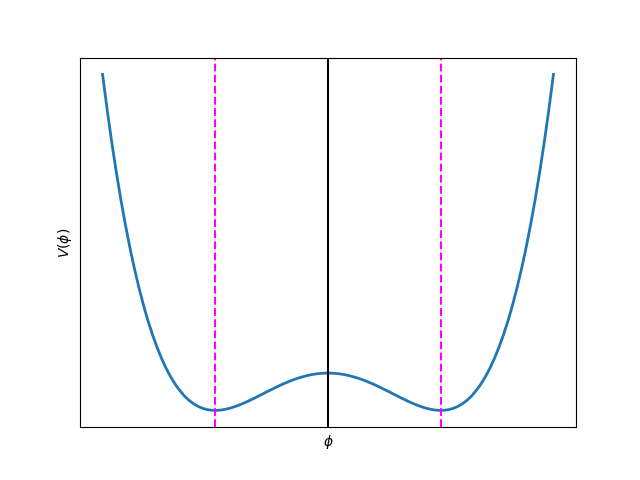
\includegraphics[scale=0.7]{figs/higgs.png}
\caption{Higgs mechanism. The dashed-magenta vertical line indicate the two vacuum states. The black vertical line is located at the origin. The minimum is not at 0, and therefore the potential has a VEV. \label{fig:higgs}}
\end{center}
\end{figure}

The gauge fields $W^\pm$ and Z acquire mass through their interaction with the Higgs boson. Thus:
\begin{equation}
W^\pm = \frac{1}{\sqrt{2}}(W^{(1)} \mp W^{(2)}), \ Z = \frac{1}{\sqrt{g_I^2 + g_Y^2}}(g_IW^{(3)} - g_Y B)
\end{equation}
Where Z and $W^\pm$ are linear combinations of the weak and hypercharge bosons (3 and 1, respectively). Then:
\begin{equation}
m_{W^\pm} = \frac{vg_I}{\sqrt{2}}, m_{Z} = v \sqrt{\frac{g_I^2 + g_Y^2}{2}}
\end{equation}
Notice that the relation between both masses is given by the so-called \textit{weak-mixing angle}, $\theta_W$
\begin{equation}
\frac{m_W^{\pm}}{m_Z} = \frac{g_I}{\sqrt(g_I + g_Y)} = \cos{\theta_W}
\end{equation}
Measured experimentally to be $\theta_W \sim 0.50 \ \rm rad$~\cite{PDG}. 

\subsection{Coupling to fermions}
The lagrangian term corresponding to the Higgs (\textit{H})-fermions (\textit{f}) interaction can be written as follows:
\begin{equation}
\mathcal{L_{Hf}} = - \lambda_e \bar{E}_L \phi E_R - \lambda_d \bar{Q}_L \phi D_{R} - \lambda_u \varepsilon^{ab} \phi_b^{\dagger}U_R + \rm h.c.
\end{equation}
Where $\lambda_e, \lambda_d$ and $\lambda_u$ are the respective coupling constants (\textit{Yukawa couplings}), different for each fermion. Substituting in this expression the Higgs field with the result obtained before:
\begin{equation}
m_e = \frac{v\lambda_e}{\sqrt{2}}, \ m_u = \frac{v\lambda_u}{\sqrt{2}}, \ m_d = \frac{v\lambda_d}{\sqrt{2}}
\end{equation}
The fermion masses are therefore proportional to the Yukawa couplings.

%%% CKM: leptonic case: interaction independent, for each flavor; not quarks
\subsection{Coupling to photons and gluons}
Both gluons and photons are gauge bosons of the strong and electromagnetic interactions, respectively. They have zero mass and spin 1. For the gluons, given that the color symmetry SU(3) is not modified by the Higgs mechanism, they don't directly interact with the Higgs boson. The only way this interaction can happen is via quark loops. 
Contrary to what happens with the gluons, the photons can interact directly with the Higgs field. Nevertheless, they don't acquire mass as a result of this interaction, $m_\gamma = 0$.  

\section{Particle Content}
\label{subsec:Particles}
%% Fermion generatio, representation in the SM gauge symmetry 
The particle content of the SM is categorized as a function of the intrinsic angular momentum of each particle, or \textit{spin}. Particles with half-integer spin are called \textit{fermions}, while those with an integer value for the spin are \textit{bosons}. The latter ones are the carriers of the different interactions that enter the SM lagrangian:
\begin{equation}
\mathcal{L} = \mathcal{L}_{kin} + \mathcal{L}_{Higgs} + \mathcal{L}_{Yuk}
\end{equation}
Where the first term accounts for the kinetic part of the interaction, and the two others describe the Higgs mechanism (described in \ref{subsec:Higgs}) and its interaction with the fermions. 
%\red{W rises when introducing the covariant derivative and explain coupling constants}
Regarding the fermions, a further classification can be made depending on whether they are affected (\textit{quarks}) or not (\textit{leptons}) by the strong interaction. If affected, a quantum number, color, further characterizes the particle. Note that the electroweak interaction affects all the particles. 

An additional quantum number, \textit{flavour}, is used to label the different elementary particles. There are three flavour families of quarks and leptons in the SM, represented in \ref{fig:particle_content}. Each lepton (electron, \textit{i}, muon, $\mu$, tauon, $\tau$) has associated a neutral particle,  called the \textit{neutrino}: $\nu_e$, $\nu_\mu$, $\nu_tau$. Even though they are predicted to be massless within the SM (so that there are not right-handed neutrinos in the SM and, equivalently, there are not left-handed antineutrinos), they are known to have mass~\cite{SolarNeutrinos}.

The elementary particles of the SM are represented in \ref{fig:particle_content}. For each of this particles, there exists another one with the same mass but opposite physical charges. Those are called \textit{antiparticles}. Notice that some particles (e.g. the photon) are their own antiparticle. 

\begin{figure} [htb!]
\begin{center}
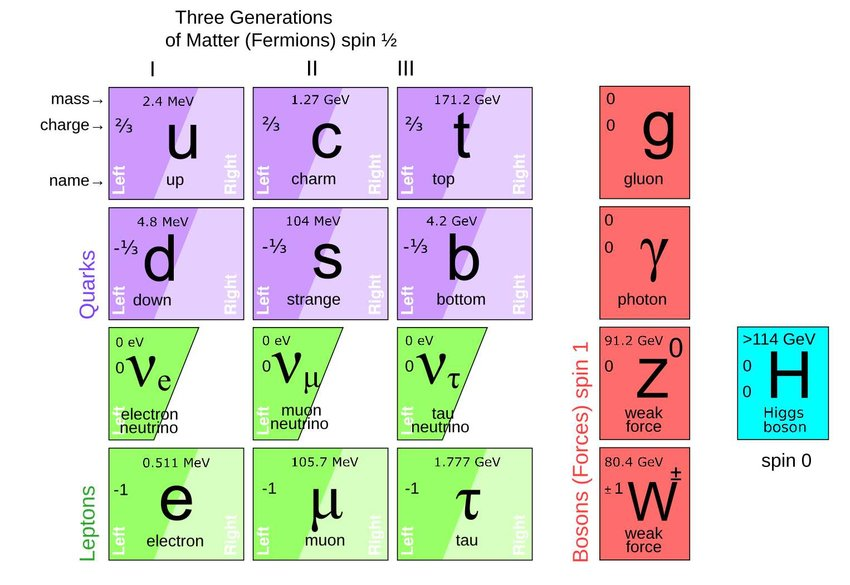
\includegraphics[scale=0.5]{figs/particle_content.jpg}
\caption{The SM particle content\red{~\cite{ParticleContent}}. \label{fig:particle_content}}
\end{center}
\end{figure}

Quarks form bound states named \textit{hadrons} that have a quantum number associated called the baryonic number, $\mathcal{B}$. They are composed either by a quark and an antiquark (forming \textit{mesons}, with $\mathcal{B} = 0$) or by three quarks (\textit{baryons}, with $\mathcal{B}=1$). Given the spin that results of the \textit{sum} of the quarks, baryons are fermions and mesons are bosons. 

\section{CKM Matrix}
\label{sec:CKMMatrix} 
The Yukawa couplings, seen in \ref{subsec:Higgs}, generate off-diagonal terms that allow for the quarks to \textit{mix} between the three generations. Diagonalizing the quark mass matrices, 4 unitary matrices are obtained, $V_{L,R}^{u,d}$, that determine the coupling of the $W^{\pm}$ bosons to the different quarks. 

This diagonalization can be seen as the rotation from one basis ($q$) to another, hereafter called \textit{mass basis} or \textit{physical basis}, $q'$. These are related by the aforementioned matrices ~\cite{CKM}:

\begin{equation}
u_L^i = V_u^{ij} u'^{j}_L \ \ d_L^i = V_d^{ij}d'^{j}_L 
\end{equation}

With this, the weak current transforms from $\bar{u}^i_L \gamma^{\mu} d_L^i$ to $\bar{u}'^i_L \gamma^{\mu}(V_u^{\dag}V_d)_{ij}) d'^i_L \equiv \bar{u}'^i_L \gamma^{\mu} V_{\rm CKM} d'^i_L$, where $V_{\rm CKM}$ is a non-diagonal, unitary matrix called the \textit{Cabibbo-Kobayashi-Maskawa} (CKM) matrix. The most up-to-date measured values of its elements can be found in~\cite{PDG}. 

\begin{equation}
V^{\rm CKM} = \begin{pmatrix}
V_{ud} & V_{us} & V_{ub}\\ 
V_{cd} & V_{cs} & V_{cb}\\ 
V_{td} & V_{ts} & V_{tb}
\end{pmatrix}
\end{equation}

This matrix is the responsible for the transitions between different quark generations, that allow for processes in which there is change in the quark flavour but not in the electric charge to happen. These are known as Flavour Changing Neutral Currents (FCNC). Most of the rare decays are of this type. It also causes CP violation, that will be discussed in the following sections. It is worth noticing that this matrix is not necessarily restricted to being 3x3, thus extra quark generations (not discovered yet) can exist~\cite{CKM}.

%\red{unitarity triangle}\red{... In QCD, flavour is a global symmetry, broken in the electroweak symmetry... }
 
%Yukawa couplings led to off-diagonal elements in the 3x3 matrix between the different families. Diagonalizing the Yukawa matrix (mass matrix), off diagonal elements appear in the charged current coupling (Q+-)
%When the three fermion generations are added to the theory, additional terms mixing quarks of different
%generations are possible. Alternatively, it is possible to diagonalise the Higgs couplings by switching
%to a different basis for the quark fields. Writing the Lagrangian in this alternative basis (hereinafter
%referred to as “mass basis” or “physical basis”) will of course simplify L Y uk but with the cost of causing
%a complication in the gauge side. Calling q the interaction eigenstates and q the mass eigenstates, both
%bases are related through the unitary relations:

\section{Need for New Physics}
%%% Introduction
Even though the SM has shown to be a very successful theory, it lacks explanation for several phenomena present in nature. 

\subsection{Matter-antimatter imbalance}
In order to have an excess of matter over antimatter in the early universe (process known as \textit{baryogenesis}~\cite{Baryogenesis}, three requirements have to be fulfilled. These are known as the \textit{Sakharov conditions}~\cite{Baryogenesis}, and include a large CP-violation. The SM predicts a rate of the CP-violation smaller than the one needed, thus, a new source is required.
%%%%%%%%%%%%%%%%%%%%%%%%%%%%%%%%%%%%%%%%%%%%%%%%%%%%%%%%%%%%%%%%%%%%%%%%%%%%%%%%%%%%%
\subsection{Dark matter and dark energy}
\label{subsec:DarkMatter_DarkEnergy}
Several experimental evidences, such as the rotational speed of spiral galaxies, gravitational lensing, or observed fluctuations in the Cosmic Microwave Background radiation (\red{see for example~\cite{DM1},~\cite{DM2}}) have lead to  discovery of dark matter and dark energy, that take up the vast majority of the Universe composition {and don't interact with light}. The possible baryonic (MACHOs, MAssive Compact Halo Objects, such as black holes, and RAMBOs, Robust Association of Massive Baryonic Objects) percentage of dark matter is small. The rest cannot be explained within the SM, it is \textit{non baryonic cold dark matter}, where cold refers to its non-relativistic nature, \red{or neutrinos}. Possible candidates for cold dark matter entail weakly interacting sub-eV particles (WISPs), such as axions(~\cite{Axions1},~\cite{Axions2},~\cite{Axions3}), primordial back holes \red{ref} and weakly interacting massive particles (WIMPs). 
%%% Experimental signatures

\subsection{Unification of forces}
The behavior of the three coupling constants at the order of TeV,\red{\textit{naturalness}}
,(figure\ref{fig:constants}, left) suggests the existence of a \textit{primary} interaction, represented by a higher symmetry group (e.g. SU(5) or SO(10)). Spontaneous symmetry breaking of this interaction would lead to the existence of the electromagnetic, weak, and strong interactions at lower energy scales. Nevertheless, in order for this to happen, there should be a matching of these coupling constants for such high energies, which is not perfectly achieved in the SM. This hints the existence of new symmetries orfields (figure\ref{fig:constants}, right). Some of these suggestions will be discussed in the following chapter. 

%% IMG source http://www.theo-physik.uni-kiel.de/~bonitz/public/nobel04/public.html
\begin{figure} [htb!]
\begin{center}
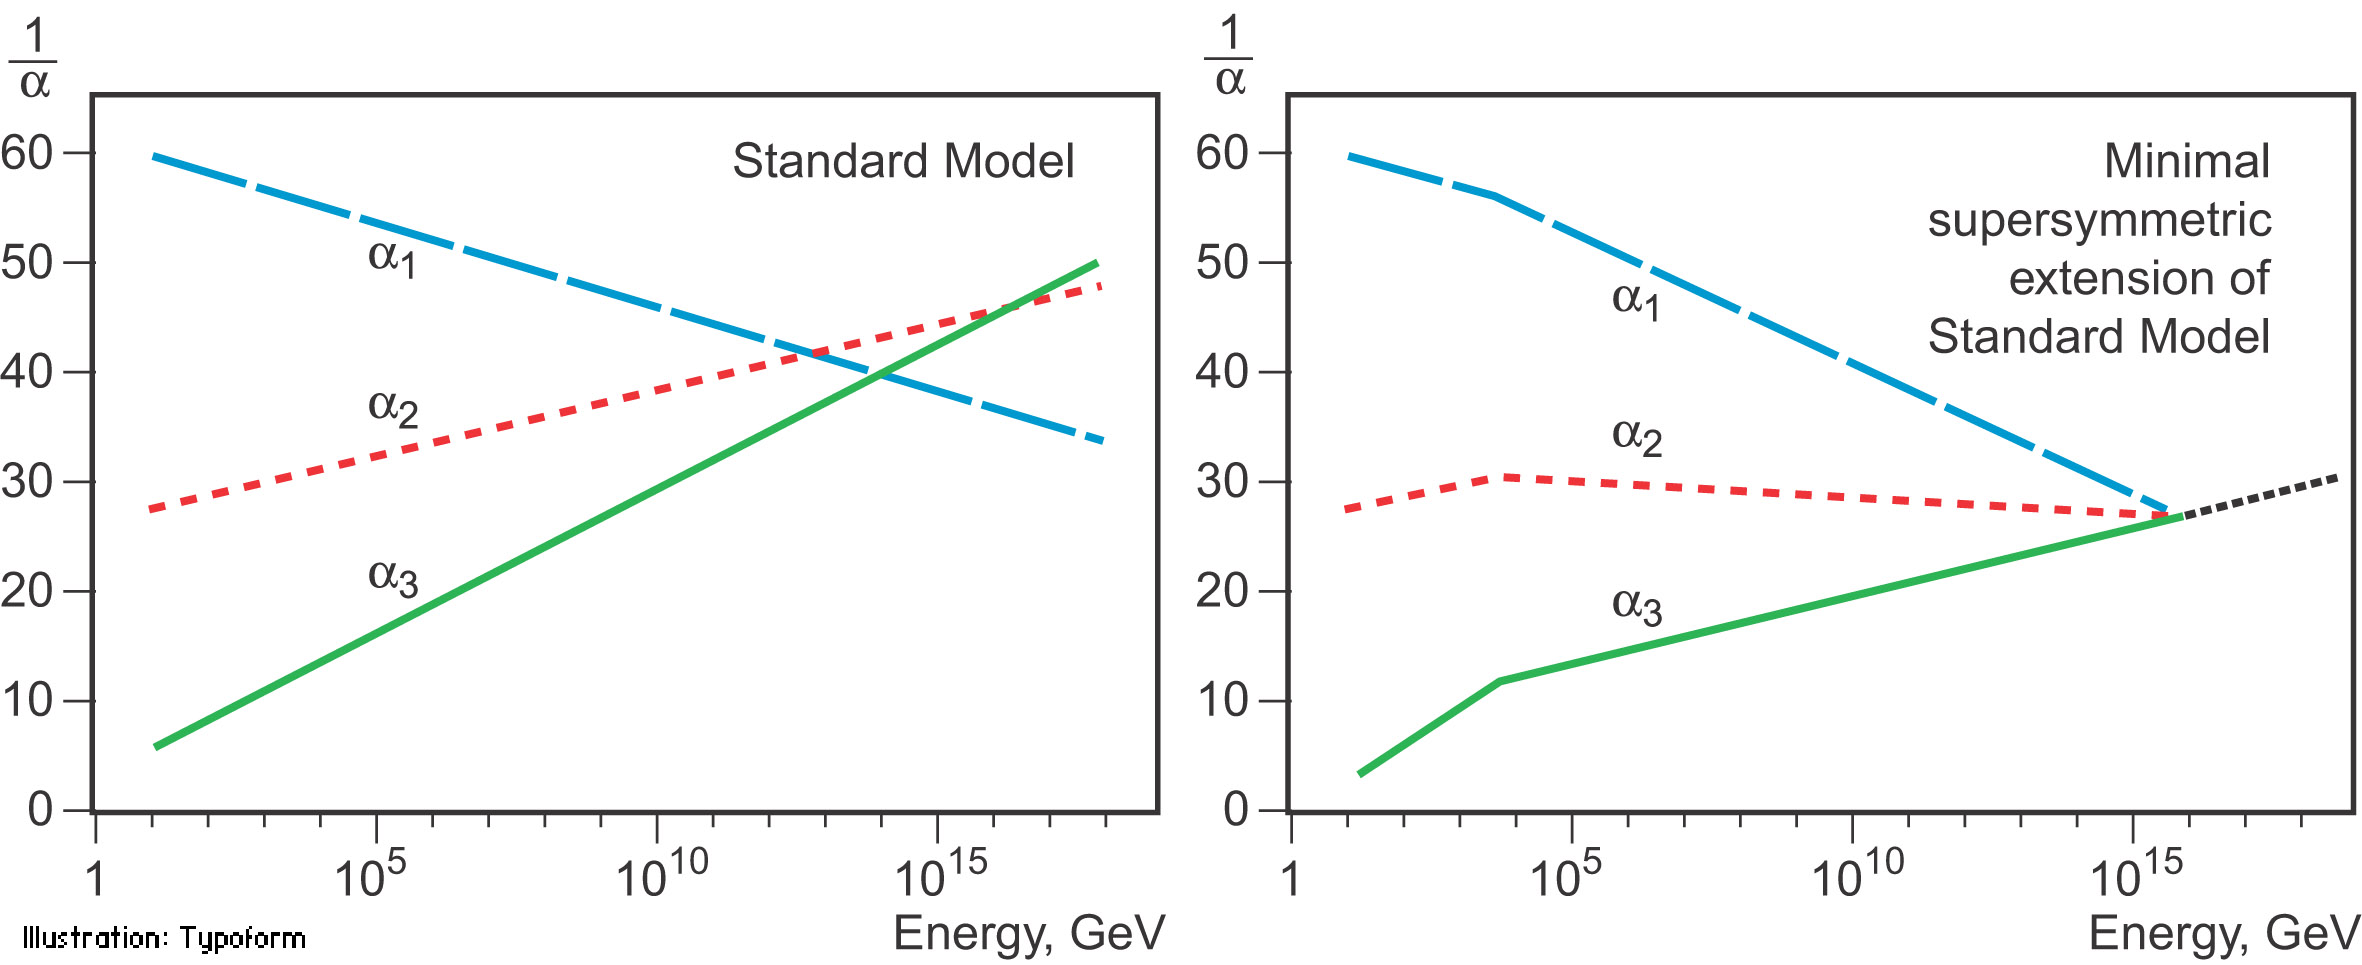
\includegraphics[scale=0.7]{figs/coupling_constants.jpg}
\caption{Running coupling constants as a function of the energy scale, for the SM (left) and in the context of supersymmetry (right)~\cite{CouplingConstants} \label{fig:constants}}
\end{center}
\end{figure}
 
\begin{itemize} 
\item The number of fermion families. As mentioned earlier, the number of fermion families is not an observable, but rather an input for the theory. More generations could in principle be accommodated as part of the SM particle content. 
\item The gauge hierarchy problem. This is intrinsically related to the mass of the Higgs boson. Apart from the fact that it is not predicted by the theory, it requires fine-tuning in order not to diverge, leading to the enlargement of the EW scale. Also, it is very small compared to the gravity scale, given by the Planck mass: $M_{Pl} = \sqrt{\hbar c/G_N} = 1.2 \times 10^{19} \GeV$, which is not fully understood. 
\item Inclusion of gravity. The SM fails to include gravity as one of the interactions, as there is no quantum theory for it. 
\item Neutrino masses. As it was already mentioned before, neutrinos are massless within the SM model. Nevertheless, experimental observations such as the oscillations of solar neutrinos\red{~\cite{SolarNeutrinos}} prove this prediction wrong. Thus, a Beyond the SM (BSM) mechanism to give neutrinos mass is required. There are several proposals for this, such as the seesaw mechanism or the Majorana theory\red{~\cite{Seesaw}}. 
\item Charge quantisation. The fact that the electron charge and the proton charge are of the same magnitude but opposite sign has no explanation in the SM. 
%\item \red{Strong CP problem}
\item Fermion masses and mixing angles. Similarly to what happened with the number of fermion families, these quantities are not predicted by the SM. Moreover, the mass of the top quark, much bigger than the other quark masses, is an intriguing fact not explained by this theory. 
\item The magnetic dipole moment of the muon, whose experimental measurement\red{~\cite{MuonDM}} deviates more than 3$\sigma$ from the SM predictions. 
\end{itemize}

In addition to this, several results provided by the LHCb collaboration \red{refs} on flavour anomalies and lepton flavour universality studies contribute to the motivation of the search for BSM physics. 

Several theories have been proposed to cope with the SM problems, that make this model look more like an effective low energy theory than a model itself. Among these, Supersymmetry and Minimal Flavour Violation (MFV) are of special importance and will be discussed in the following chapters. However, there are other alternatives, some of which are briefly discussed below.

\begin{itemize}
\item \textbf{Majorana neutrinos}: in the SM, neutrinos are supposed to be massless \textit{Dirac} particles. However it's been suggested that they are instead its own antiparticle, \textit{Majorana neutrinos}. Within this theory, they are allowed to acquire mass. Several experiments search for a neutrinoless double beta decay that would prove this~\cite{KamLAND-Zen:2016pfg},~\cite{GERDA}.
\item \textbf{Axions}: axions are hypothetical particles that compose DM, including the Peccei-Quinn mechanism~\cite{Axions1} to solve the \red{strong CP problem}~\cite{StrongCP}. They would have been massively produced soon after the Big Bang. The couplings and masses axions can cover several orders of magnitudes. %%%https://arxiv.org/pdf/1712.03018.pdf %% http://iaxo.web.cern.ch/content/physics
\item \textbf{Two Higgs Doublet Models (THDM)}: in this scenario, there are two Higgs fields populating the vacuum instead of one. %% https://arxiv.org/pdf/1106.0034.pdf
\begin{equation}
\left \langle \phi_a \right \rangle_0 = \binom{0}{\frac{v_1}{\sqrt{2}}}, \ \left \langle \phi_b \right \rangle_0 = \binom{0}{\frac{v_2}{\sqrt{2}}}
\end{equation}
Where $v_2$ and $v_2$ follow the relation:
\begin{equation}
v \equiv (v_1^2 + v_2^2)^{1/2}
\end{equation}
The ratio between these two VEVs, $\tan{\beta} \equiv \frac{v_2}{v_1}$ is the most important parameter in this model. It describes the diagonalization of the mass-squared matrices of the charged scalars and of the pseudoscalars, resulting in 4 fields
\begin{equation}
\begin{split}
& \phi_1 = \sin{\beta}\phi_b + \cos{\beta}\phi_a \ \phi_2 = -\sin{\beta}\phi_a + \cos{\beta}\phi_b \\
& \left \langle \phi_1 \right \rangle_0 = \binom{0}{\frac{v_{SM}}{\sqrt{2}}}, \ \left \langle \phi_2 \right \rangle_0 = \binom{0}{0}
\end{split}
\end{equation}
The spontaneous symmetry breaking leads in this case to 5 physical Higgs particles: two neutral scalars linear combinations of $Re(\phi_1^0)$ and $Re(\phi_1^0)$, $H^0$ and $h^0$; a neutral pseudoscalar, $A^0 \propto Im(\phi_2^0)$ and two charged scalars $H^\pm = \phi_2^\pm$.  
\item \textbf{Models with extra dimensions}: models with extra dimensions (apart from the usual 4 from the observed spacetime) are motivated by the attempts made to unify electromagnetism and gravity within the Kaluza-Klein theory~\cite{Kaluza},~\cite{Klein}. There are several proposals, such as \textit{string theory} or the \textit{Randall-Sundrum model}~\cite{RS}, that gives explanation to hierarchy using 5 dimensions and predicts the existence of the \textit{graviton}. 
\item \textbf{SM with fourth generation (SM4)}: adding a fourth generation of fermions requires the corresponding neutrino to be heavy, $m_{\nu_4} > M_Z/2$, to match the current experimental constraints~\cite{Lenz:2013iha}.   %%https://cds.cern.ch/record/1635712/files/910275.pdf
\item \textbf{Little Higgs Models}: in these models, the Higgs is realised as a light pseudo-Nambu Goldstone boson of a broken global symmetry. They attempt to solve the gauge hierarchy problem. The minimal version of such models include 4 new heavy vector bosons, ($W'^{\pm}$, $Z'$, $B'$), coupled to SM fermions, mixed with the SM $W^{\pm}$ and $Z$;  light Higgs doublet(s), with possibility of extra light scalar multiplets; heavy Higgs multiplets, coupled to Higgs/Goldstone pairs, decoupled from fermions, mixed with light Higgses, and heavy up-type quark(s), $t'$. An example spectrum can be seen in \ref{fig:lhm}. Updated constraints in this model can be found in~\cite{LHM}.
   %%https://arxiv.org/pdf/1703.10190.pdf %%http://www.desy.de/~reuter/downloads/lhm.pdf
\begin{figure} [htb!]
\begin{center}
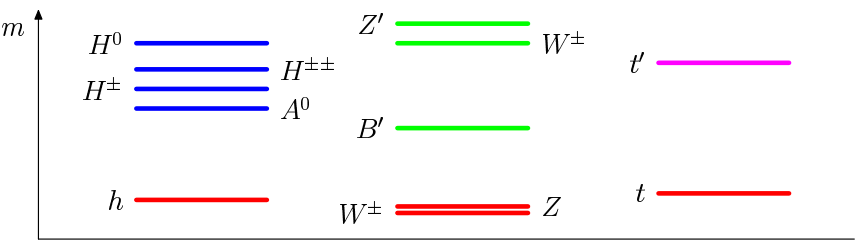
\includegraphics[scale=0.7]{figs/lhm.png}
\caption{Example spectrum for LHM \red{ref?} \label{fig:lhm}}
\end{center}
\end{figure}
\end{itemize}


\chapter{Supersymmetry}
\label{sec:sup}
\section{Introduction}
\label{sec:introduction}%%%kazakov 2006, theory and phenomenology of sparticles, guía d e la teoría cuántica de campos 
Supersymmetry (henceforth SUSY) is a framework that constitutes one of the main alternatives for BSM Physics. Postulated in the \red{70s} as a graded Lie algebra (with conmutators and anticonmutators), allowed by the Coleman-Mandula theorem ~\cite{ColemanMandula}, possess a unique mathematical nature that allows for the solution of several of the SM caveats that were discussed in the chapter before. It is being searched for in several experiments, and not yet discovered. Lower limits are set in the scale of SUSY breaking, the so-called scale of new physics. \red{current bounds?}  

SUSY can be seen as a generalization of space-time symmetries in QFT, establishing an invariance under the transformations of fermions to bosons, requiring their number to be the same in nature. Hence, for each boson (fermion) there is a superpartner of fermionic (bosonic) nature. If SUSY wasn't broken, the symmetry would be exact and the masses of the particles would coincide with those of their respective superpartners, which is not observed in nature. Moreover, none of the particles known to date fulfills the quality to be a superpartner, which leads to the conclusion that for Supersymmetry to exist there must be more particles than those seen so far (the double, in the simplest supersymmetric extension of the SM). 

A new quantity number can be introduced within SUSY, R-parity, defined as:
\begin{equation}
R = (-1)^{3B + L + 2S}
\end{equation}
Where B is the baryon number, L the lepton number (both quantities conerved in the SM) and S the spin. Particles with R = 1 are SM particles, while their superpartners have R = -1. Models where R-Parity is conserved (hence, B-L invariance) predict the production of superparticle in pairs, and at least one stable supersymmetric particle, the Lightest Supersymmetric Particle (LSP), thus providing a good candidatefor dark matter. There are also SUSY models where R-parity is violated, allowing the LSP to decay to SM particles. An example of a RPVmodel is the bilinear RPV CMSSM~\cite{RPVCMSSM}.%%% https://indico.cern.ch/event/389531/contributions/929493/attachments/1147997/1646586/RPV-status.pdf,

\section{Points addressed by SUSY}
\label{sec:SUSYpoints}
As mentioned earlier, the success of SUSY lies in the coverage of SM most important \red{pitfalls}. A summary of this is discussed in this section. 
\begin{itemize}
\item \textbf{Unification of forces}: as explained in the \ref{sec:introduction}, gravity is not included in the SM. Nevertheless, given that SUSY algebra is a generalization of Poincaré algebra, it is therefore invariant under general coordinate transformation if it is local. With this, a theory including gravity ({\textit{supergravity}}) can be obtained from SUSY. 
\item \textbf{Gauge hierarchy problem}: Supersymmetry (and supersymmetric partners) lead to the cancellation of quadratic mass terms causing divergences up to the SUSY breaking scale, $M_{SUSY}$, given the relation 
\begin{equation}
\sum_{bosons} m^2 - \sum_{fermions} m^2 = M_{SUSY}^2
\end{equation}
\red{The origin of EWSB can also be explained from radiative electroweak symmetry breaking within SUSY, also explaining the difference between the scales ($M_{SUSY}$ and the Higgs mass).}
\item \textbf{Unification of forces}: as mentioned earlier, the behavior of the coupling constants at high energies hints a \textit{great unification} of forces. This match, while not perfect in the SM, is obtained in a supersymmetric scenario, as it can be seen in figure~\ref{fig:constants}, thanks to the change in the parameters of the renormalization group equations. 
\item \textbf{Matter-antimatter imbalance}: leptogenesis (a scenario in which there is an asymmetry between leptons and antileptons in the early universe) can happen in RPV models, being able to accomnodate the total matter-antimatter imbalance. %%% \red{seesaw mechanism?}%%hypothetical massive bosons leptogenesis? %% https://arxiv.org/pdf/1206.3168.pdf, https://arxiv.org/pdf/0802.2962.pdf
\item \textbf{Dark matter and dark energy}: as pointed out in~\ref{subsec:DarkMatter_DarkEnergy}, most of the origin of dark matter and dark energy remains unexplained in the SM. Supersymmetry can provide several candidates for this, provided R-parity is conserved. More details on the possibilities are discussed in \red{ref}.
\end{itemize}

\section{Supersymmetry breaking} %% theory and phenomenology of susy particles
\label{sec:SUSYbreak}
Supersymmetry breaking is inferred from experimental observation. Without it, the abundance and mass of partners and superpartners would be equal,as said in \ref{sec:introduction}. Moreover, experimental constraints can help reducing the arbitrariness of the MSSM parameters. 

All global continuous symmetries can be broken with an \textit{extra} component of the Lagrangian that breaks the symmetry of the larger part (Heisenberg-Wigner mode), with spontaneous symmetry breaking and the resulting appearance of Goldstone particles, or with a combination of these two methods. The Minimal Supersymmetric Standard Model is an example of the former, and will be discussed in more detail in the following section. 

\section{Minimal Supersymmetrical Standard Model (MSSM)}
\label{sec:MSSM}
The Minimal Supersymmetrical Standard Model is the simplest supersymmetric extension of the SM, containing some general features that do not depend on the choice of model. Among said features is the fact that for each SM partner there is a \textit{superpartner} (\textit{gauginos} for bosons and \textit{sfermions} for fermions), with spin differing 1/2. The particle content is summarized in \ref{tab:parMSSM}.

\begin{table}[h]
  \begin{center}
     \caption{Particle content of the MSSM}
  \label{tab:parMSSM}
  \begin{tabular}{|c|c|c|}
  \hline
  SM & MSSM & Spin \\
    \hline
    gluon ($g$) & gluino $\tilde{g}$ & 1/2\\
    Hypercharge \& Weak bosons & $\tilde{W}^0,\tilde{W}^{\pm}, \tilde{B}^0$ & 1/2 \\
    leptons ($(\nu, l)_L$, $e_R$) & sleptons ($(\tilde{\nu},\tilde{l})_L$, $\tilde{e}_R$) & 0\\
    quarks ($q$) & squarks ($\tilde{q}$) & 0\\
    Higgs field & Higgsinos ($\tilde{H}_u^{\pm}$, $\tilde{H}_d^{\pm}$, $\tilde{H}_u^{0}$, $\tilde{H}_d^{0}$) & 1/2\\
    \hline
  \end{tabular}
  \end{center}
\end{table}

Notice that in the MSSM, as in any supersymmetric scenario, it is required the presence of 2 Higgs bosons in the SM with hypercharge -1 and 1, \red{compatible with FCNC constraints}, as it fulfills the Glashow-Weinberg/Paschos condition(~\cite{Pascos1}, ~\cite{Pascos2}).  Gauginos have spin zero in order to be matter scalars and not gauge bosons. As for the sfermions, the only consistent interacting field theory of spin 3/2 has to include gravity\red{~\cite{Freedman:1976xh}}, hence they have spin 1/2. This theory, known as \textit{supergravity}, includes the superpartner of the \textit{graviton}, known as \textit{gravitino}. It is also worth mentioning that the MSSM, like the SM, fails to explain the number of fermion families. 

The MSSM has some interesing features, such as the improvement in the unification of gauge coupling constants at some high energy scale, $\Lambda$ ,still undetermined but known to be  in the order of $2\times10^{16}$ GeV. This unification is kept if SUSY isbroken at a scale $M_S \leq \mathcal{O} (1 \rm TeV)$. Even if gravity is included, its coupling constant seems to roughly point to the same value at the same $\Lambda$.

%%%% the goal of the BSM search is to find evidence for effects that are present in the theory with a finite value of Lambda, but disappear in the limit Lambda goes to infinity. Limits on electron and neutron EDM require the scale to be larger than 10^7 GeV, while the KK bar mass difference sets a lower bound of about 10^6 GeV on the scale of DS = 2 flavour transitions 

The soft-explicit breaking of the MSSM (or the electroweak symmetry breaking itself) allows for mixing between different sparticles with the same charge and color to happen. This leads to the existence of \textit{charginos} ($\tilde{\chi}^{\pm}_{1,2}$) and \textit{neutralinos} ($\tilde{\chi}^{0}_{1,2,3,4}$), as a combination of gauginos and higgsinos for the former and neutral gauginos for the latter. Sfermion mixing can also happen. \textcolor{blue}{The mixing patterns and mass values of sparticle mass eigenstates depend crucially on the manner of supersymmetry breaking.} 

\subsection{Dark Matter in the MSSM}
%% Introduction
As said before, within the SUSY framework there are several candidates to constitute DM. A common feature they share is their stability. These candidates are:
\begin{itemize}
\item Sneutrino: ruled out in the MSSM because of the current limits on the interaction cross section of dark matter particles with ordinary matter as measured by direct detection experiments
\item Lightest neutralino: the LSP for models conserving R-parity. Depending on its composition it can be of different natures. Said composition comes determined by a unitary 4x4 matrix that diagonalize the neutralino mass matrix, $N$, as seen in \ref{eq:Nneutralino}. \ref{eq:neu1composition}. 
\begin{enumerate}
\item Bino-like: when the term $N_{11}$ dominates the neutralino diagonalization matrix, $N$, fulfilled for $M_1 < \mu$
\item Higgsino-like: when the off-diagonal elements in the mixing matrix ($N_{13}^2 + N_{14}^2$) dominate, for $\mu < M1$ 
\item Wino-like: when the term $N_{12}$ dominates the neutralino diagonalization matrix, $N$, fulfilled for $\mu, M_{1,3} < M_2$
\item Mixed states of the above 
\end{enumerate}
\item Gravitino
\end{itemize}

%%% neutralino mass matrix
\begin{equation}
\left( \begin{matrix}
N_{11} & N_{12} & N_{13} & N_{14} \\ 
N_{21} & N_{22} & N_{23} & N_{24} \\
N_{31} & N_{32} & N_{33} & N_{34} \\ 
N_{41} & N_{42} & N_{43} & N_{44} \\
\end{matrix}\right)
\label{eq:Nneutralino}
\end{equation}

\begin{equation}
\chi_1^0 = N_{11}\tilde{B} + N_{12}\tilde{W} + N_{13} \tilde{H}_d^0 + N_{14}\tilde{H}_u^0
\label{eq:neu1composition}
\end{equation}
%%https://arxiv.org/pdf/1804.05238.pdf

\subsection{MSSM Lagrangian}
\label{sec:MSSMLag}
The MSSM lagrangiang consists of two parts:

\begin{equation}
\mathcal{L}_{\rm MSSM} = \mathcal{L}_{\rm SUSY} + \mathcal{L}_{\rm SOFT}
\end{equation}

Where the first part is just a generalization of the SM lagrangian, and the second part contains the supersymmetry breaking mechanism. 
The corresponding \textit{superpotential} used in $\mathcal{L}_{rm SUSY}$ is of the form:

\begin{equation}
W = \epsilon_{ij}(y_{ab}^{U}Q_a^jU_b^cH_2^i + y_{ab}^{D}Q_a^j D_b^c H_1^i + y_{ab}^{L} L_a^j E_b^c H_1^i + \mu H_1^i H_2^j)
\label{eq:superpotential}
\end{equation}

Where $Q$, $U$ and $D$ represent the squark superfields, $L$ and $E$ the \red{slepton} ones, $y^{U,D,L}$ are the Yukawa couplings and $H_{1,2}$ the Higgs superfields. The only qualitative difference with respect to $\mathcal{L}_{\rm SM}$ is the last term, that accounts for the Higgs mixing. Additional lepton violating leptonic or baryonic number can be added to this superpotential in RPV models. 

Because of gauge invariance, supersymmetry breaking in the MSSM cannot \red{happen spontaneously}. Thus, an explicit term accounting for this breaking appears in the lagrangian, $\mathcal{L}_{\rm SOFT}$, where \textit{soft} refers to the dimension 2 and 3 of the operators.  This breaking is the responsible for the SM particles not to be degenerate with their respective superpartners, as mentioned earlier, having these larger masses. \red{Nonetheless this SUSY breaking, some properties from it remain.} 

%%% singlets?
A possible alternative to the soft-explicit supersymmetry breaking explained before consists in spontaneous symmetry breaking for a given scale, $\Lambda_s$, with a sector of fields that belong to a \textit{hidden} sector and communicates with the \textit{observable} sector with the exchange of fields known as \textit{messengers}, as represented schematically in \ref{fig:hiddensector}. This type of supersymmetry has been extensively searched for in several experiments, with negative results so far \red{REFERENCES}.

\begin{figure} [htb!]
\begin{center}
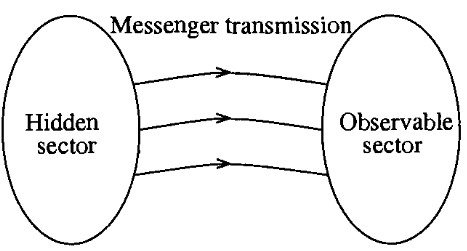
\includegraphics[scale=0.5]{figs/hidden_sector.png}
\caption{Schematic view of the hidden sector \label{fig:hiddensector}}
\end{center}
\end{figure}

The MSSM has 124 free parameters, namely:

\begin{itemize}
\item 18 SM parameters
\item 1 Higgs sector parameter, analogue to the SM Higgs mass
\item 5 real and 3 CP violating phases in the gaugino/higgsino sector
\item 21 squark and slepton masses
\item 36 real mixing angles for squark and slepton mass eigenstates
\item real mixing angles for squark and slepton mass eigenstates
\end{itemize}

The complex phases are usually considered small. Some experiments are capable of measuring some of these parameters individually. Nevertheless, in general this large amount of degrees of freedom \red{spoil the predictive power of the model}. In order to reduce it, \textit{mass universality} is imposed to some particular cases that will be further discussed in the next section. This implies that all spin 0 (1/2) sparticle masses are equal to a universal value $m_0$ ($m_{1/2}$). Another way of reducing the number of parameters is specifying the mechanism that breaks the symmetry, either with gauge fields (Gauge Mediated Supersymmetry Breaking, GMSB)[40] or as a consequence of a dominating super-Weyl anomaly (Anomaly Mediated Supersymmetry Breaking, AMSB). Some of this models will be explained in more detail later. 

%%% Revisar notas --30min

%%% TOTAL: 2h, 2h por la tarde, 2h mañana 


%-- Reduce arbitrariness in the choice of the MSSM parameters  => impose constraints 
%	-- gauge coupling constant unification 
%	-- mZ from EWSB 
%	-- Yukawa copling constant unification 
%	-- Precision measurement of decay rates
%	-- Anomalous magnetic moment of the muon 
%	-- Lower limits on SUSY masses
%	-- DM constraint 
\subsection{CMSSM}
\label{sec:CMSSM}
%% http://www.hep.ph.ic.ac.uk/~tapper/lecture/susy-lecture-1.pdf
%% https://indico.cern.ch/event/136806/contributions/143942/attachments/112092/159367/Wells.pdf
%% http://www.desy.de/~reuter/downloads/marialaach_susy07.pdf
The \textit{constrained} MSSM (hereafter CMSSM) is one of the most popular subversions of the MSSM. In this model, the concept introduced earlier of mass universality is imposed, meaning that for a given GUT scale $\Lambda \sim 2\times 10^{16} \rm GeV$:
\begin{itemize}
\item All scalar masses are set to $m_0$
\begin{equation}
M_{\tilde{l}}^2(\Lambda) = M_{\tilde{q}}^2(\Lambda) \equiv m_0^2 I_3
\end{equation}
\begin{equation}
M_{\tilde{u}}^2(\Lambda) = M_{\tilde{e}}^2(\Lambda) = M_{\tilde{d}}^2(\Lambda) \equiv m_0^2 I_3
\end{equation}
\begin{equation}
m_{H_u}^2 = m_{H_d}^2 = m_0^2
\end{equation}
Where $I_3$ represents the 3x3 identity matrix
\item All gaugino masses are set to $m_{1/2}$
\begin{equation}
m_{\tilde{B}}(\Lambda) = m_{\tilde{W}}(\Lambda) = m_{\tilde{g}}(\Lambda) \equiv m_{1/2}
\end{equation}
\item The trilinear couplings are set to $A_0$
\begin{equation}
A_{\tilde{u}}(\Lambda) = A_{\tilde{e}}(\Lambda) = A_{\tilde{d}}(\Lambda) \equiv A_0 I_3
\end{equation}
\end{itemize} 
These requirements lead to the following relation between the gaugino masses at the TeV scale: 
%\begin{equation} 
%M_{\tilde{g}} : M_{\rm char} : M_{\rm neu} \sim 6 : 4 : 1
%\end{equation}
\begin{equation}
M_1 = \frac{\alpha_s}{\alpha} \sin{\theta_W}^2 M_2 = \frac{3}{5}\cos{\theta_W}^2 M_1
\end{equation}
Which translates into the ratios:
\begin{equation}
M_1 : M_2 : M_3 \approx 1 : 2 : 6
\end{equation}

With these conditions, the CMSSM ends up with a set of 5 free parameters: ($m_0$, $m_{1/2}$, $A_0$, $\tan{\beta} = \frac{v_1}{v_2}$, $\rm sign(\mu)$). The last one refers to the sign of the Higgs self-coupling in the superpotential, while $\tan{\beta} = \frac{v_u}{v_d}$ is the ratio of the vevs from the Higgs doublet. Since gaugino masses run in the same way as the gauge couplings, within the CMSSM the LSP is generally the lightest neutralino. The status of CMSSM in light of current experimental constraints will be reviewed in chapter \ref{sec:CMSSM}.  %% .  \red{supersymmetry invariant higgsino mass? (book)}

%%% main uncertainty comes from the unknown soft terms
%% LSP stable, so that relic neutralinos might survive in the Universe since the Big Bang 
A more restrictive version of CMSSM exists, mSUGRA, where supersymmetry breaking is gravity-mediated. Within this model, the gravitino mass is equal to the scalar mass, $m_{3/2} = m_0$, thus adding a new constraint on the parameters. On the contrary, there are models with more relaxed conditions. An example of these is when the universality condition on the Higgs masses is not applied, hence having Non Universal Higgs Masses (NUHM1 and NUHM2~\cite{Ellis:2002wv}). This adds two extra free parameters, $M_A$, the mass of the CP-odd neutral higgs, $A^0$, and $\mu$, the Higgs self-coupling.  %%%relax the universality conditions on the Higgs masses  on the Higgs mass, 

\subsection{AMSB}
\label{sec:AMSB}
%% Definition : marron
%% mAMSB : blue
%%% Characteristics : red
In the Anomaly Mediated SUSY Breaking (AMSB), the supersymmetry breaking occurs mainly via a loop-induced super-Weyl anomaly. In some scenarios, such breaking is assumed to take place in a different \textit{brane} from respect to the \textit{observable} sector, within the context of \textit{Extra Dimensions}. \textcolor{blue}{The anomaly-mediated SUSY breaking parameters are RG-invariant, being the corresponding masses given as functions of the gauge and Yukawa coupling constants. This helps avoiding a SUSY flavor problem.}

To generate the weak scale masses of the sparticles, the gravitino mass, $m_{3/2}$ must be fairly heavy (of the order of tens of TeV). Ths, it's not affected by Big-Bang nucleosynthesis bounds.  
The gaugino masses $M_{1,2,3}$ are suppressed by loop factors relative to this gravitino mass, and the \red{wino-like states are lighter than the bino-like ones}. The following approximate ratios hold:
\begin{equation}
|M_1| : |M_2| : |M_3| \approx 2.8 : 1 : 7.1
\end{equation}

Within this model, the soft supersymmetry breaking terms can be computed from the gravitino mass, and the soft terms are real and both flavor and renormalization group invariant.
Despite its many advantages, AMSB has a strong drawback: renormalization leads to negative squared masses for sleptons. There are several proposals to cope with this, like the \textit{minimal} AMSB (mAMSB), that will be discussed further in \ref{sec:mAMSB}.

\subsubsection{mAMSB}
\label{sec:mAMSB}

In mAMSB, with the purpose of avoiding \textit{tachyonic} sleptons in AMSB models, a constant contribution ($m_0^2$) is added to all squared scalar masses a the grand unified theory (GUT) scale, $\Lambda_{GUT} \sim 2 \time 10^{16} \rm GeV$. This addition can be mostly related to the presence of extra field(s)in the bulk~\cite{Datta:2001er}, and destroys the aforementioned RG invariance, desirable in order to fulfill the \red{Flavour-Changing-Neutrl-Current (FCNC)} constraint. Nevertheless some characteristics are inherited. 


Both the $\mu$ term and the  to match soft bilinear Higgs coupling, $B_{\mu}$ are parameters of this model too. Given that they determine the Higgs potential:
\begin{equation}
G_F = [2\sqrt{2}(v_2^2 + v_1^1)]^{-1} \simeq 1.7 \times 10^{-5} \rm GeV^{-2}
\label{eq:higgspotential}
\end{equation}
The minimization of \ref{eq:higgspotential} leads to the determination of such paramaters as a function of $\tan{\beta}$. Therefore, the mAMSB model has 3 continuous free parameters, ($m_0$, $m_{3/2}$, $\tan{\beta}$). In addition, the sign of the Higgsino mixing parameter, $\mu$,  is also free. The trilinear soft SUSY-breaking mass terms, like the gaugino masses, are determined by anomalies, therefore they are proportional to the gravitino mass.  

This model has some interesting features, such as:
\begin{itemize}
\item The left and right sleptons are nearly degenerate ($m_{\tilde{l}_R} \approx m_{\tilde{l}_L}$), being stau the lightest slepton. As a consequence, the third and second generation \textit{L-R} mixing angles become significantly larger, reaching the maximal limit at large $\tan{\beta}$.
\item The lightest chargino and neutralino are also almost degenerate ($m_{\tilde{\chi}_1^{\pm}} \approx m_{\tilde{\chi}_1^0}$). This induces to a relatively long-lived $\tilde{\chi}_1^{\pm}$, that decays to a soft charged pion. 
\item Sfermion masses increase lineraly with $m_0$, but also depend on the precise value of $m_{3/2}$.
\item The mass hierarchy between sleptons and gauginos depends on the input parameters.
\item The squark masses are typically very heavy, as they grow with $g_3^4m_{3/2}^2$.
\item The stop masses are relatively high, because of the Higgs mass and the relatively low values of the trilinear couplings.
\item The LSP (lightest neutralino) can be wino-, Higgsino-like or mixed-
\end{itemize}

The most up-to-date likelihood analysis of this model in light of current constraints can be found in~\cite{Bagnaschi:2016xfg}. 
A complete spectra at the best-fit points for the two signs of $\mu$ are shown in Fig. \ref{fig:spectrumno} in the wino-LSP case, where branching ratios exceeding 20\% are indicated by dashed lines. As itcan be seen, a relatively heavy spectrum is favoured in the global fit.
\begin{figure}[htb!]
\begin{center}
  \resizebox{7.5cm}{!}{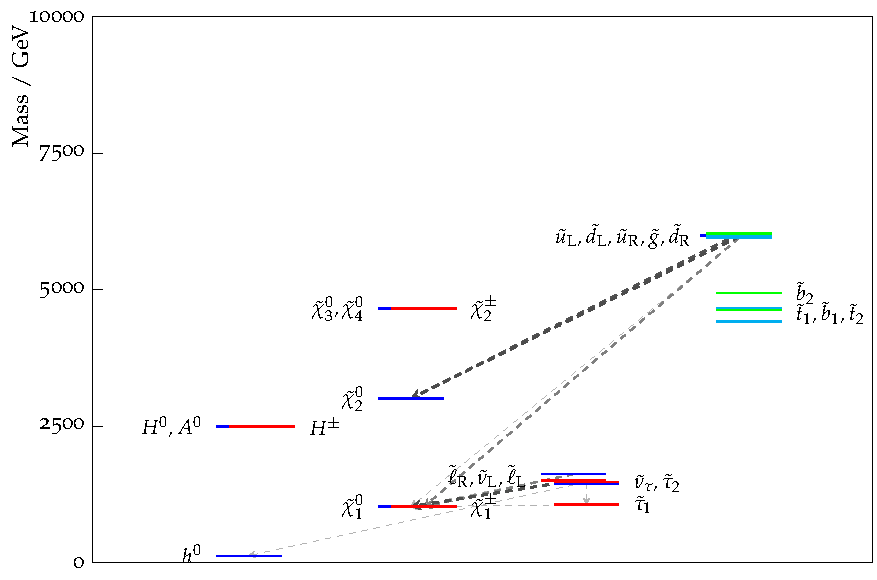
\includegraphics{figs/bfp_posmu_noDM_w_slha.pdf}}\put(-174, +144){\small $\tilde{W}$-LSP  for $\mu>0$, $\Omega_{\tilde{\chi}_1^0}<\Omega_{\rm CDM}$}%above figure
  \resizebox{7.5cm}{!}{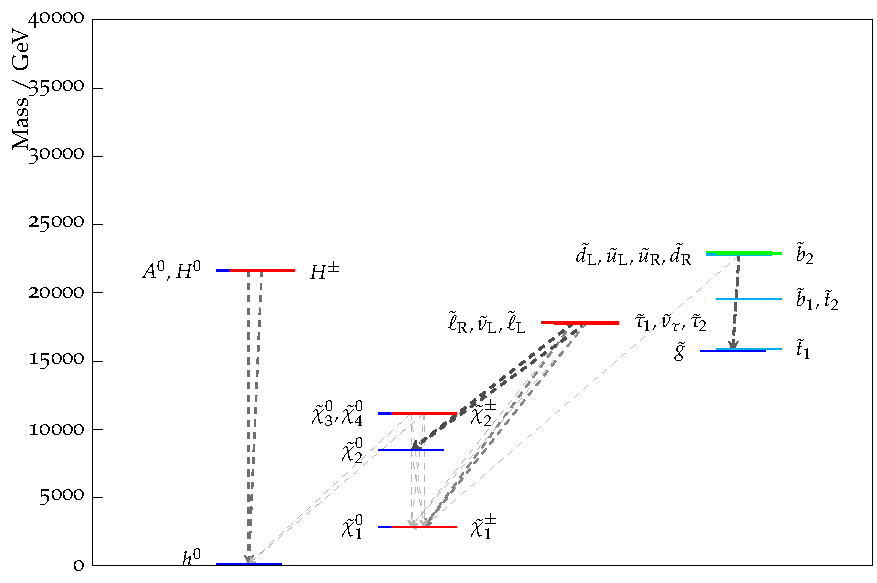
\includegraphics{figs/bfp_negmu_noDM_w_slha.pdf}}\put(-174, +144){\small  $\tilde{W}$-LSP  for $\mu<0$, $\Omega_{\tilde{\chi}_1^0}<\Omega_{\rm CDM}$}%above figure
%\vspace{0.5cm}
%\resizebox{7.5cm}{!}{\includegraphics{bfp_posmu_noDM_h_slha.pdf}}\put(-174, +144){\small  $\tilde{H}$-LSP  for $\mu>0$, $\Omega_{\neu1}<\Omega_{\rm CDM}$}%above figure
%\resizebox{7.5cm}{!}{\includegraphics{bfp_negmu_noDM_h_slha.pdf}}\put(-174, +144){\small  $\tilde{H}$-LSP  for $\mu<0$, $\Omega_{\neu1}<\Omega_{\rm CDM}$}%above figure
\end{center}
\vspace{-0.5cm}
\caption{The spectra of the best-fit points for $\mu > 0$, allowing the LSP to contribute only part of the cold dark matter density. The wino--like LSP (lower) best-fit point is shown, indicating all the decay modes with branching ratios (BRs) above 20\%, with darker shading for larger BRs, and the colours of the horizontal bars reflect particles¿ electric charges.}
%{The range of masses shown for the $\tilde{W}$-LSP $\mu>0$ best fit point (top-left panel) is smaller than the others, since its mass spectrum is considerably lighter.} } }
\label{fig:spectrumno}
\end{figure}

The preferred regions of the $(m_0, m_{3/2})$ planes for $\mu > 0$ (left panel) and $\mu < 0$ (right panel)are shown in  the upper panels of Fig \ref{fig:m0m32UL}~\footnote{{The sharp boundaries at low $m_0$ in the upper panels of Fig \ref{fig:m0m32UL} are due to the stau becoming {the LSP}, and the narrow separation between the near-horizontal portions of the 68 and 95\% CL contours
in the upper right panel of Fig. \ref{fig:m0m32UL} is due to the sharp upper limit on the CDM density.}}. 
It is seen that the wino region allowed at the 95\% CL extends to smaller $m_{3/2}$ for both signs of $\mu$, and also to larger $m_0$ at $m_{3/2} \gtrsim 300 \rm TeV$ when $\mu < 0$. The 68\% CL region extends to much larger $m_0$ and $m_{3/2}$
when $\mu < 0$, and the best-fit point also moves to larger masses than for $\mu > 0$, {though with smaller $\tan{\beta}$}.

\begin{figure}[htb!]
\vspace{0.5cm}
\begin{center}
\resizebox{7.5cm}{!}{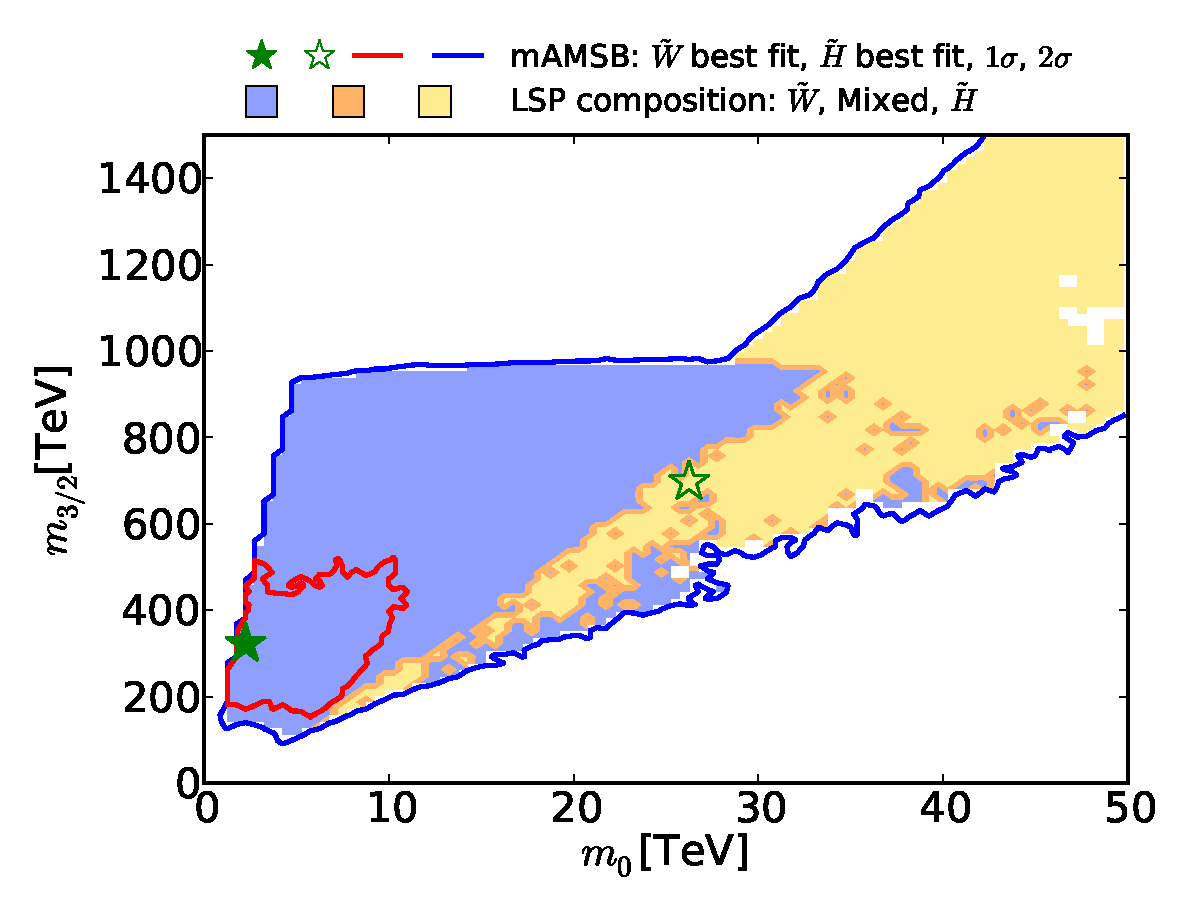
\includegraphics{figs/posmu_noDM_m0TeV50_m32TeV1500_chi2.pdf}}\put(-169, +123){\footnotesize $\mu>0$, $\Omega_{\tilde{\chi}_1^0}<\Omega_{\rm CDM}$}%top left
\resizebox{7.5cm}{!}{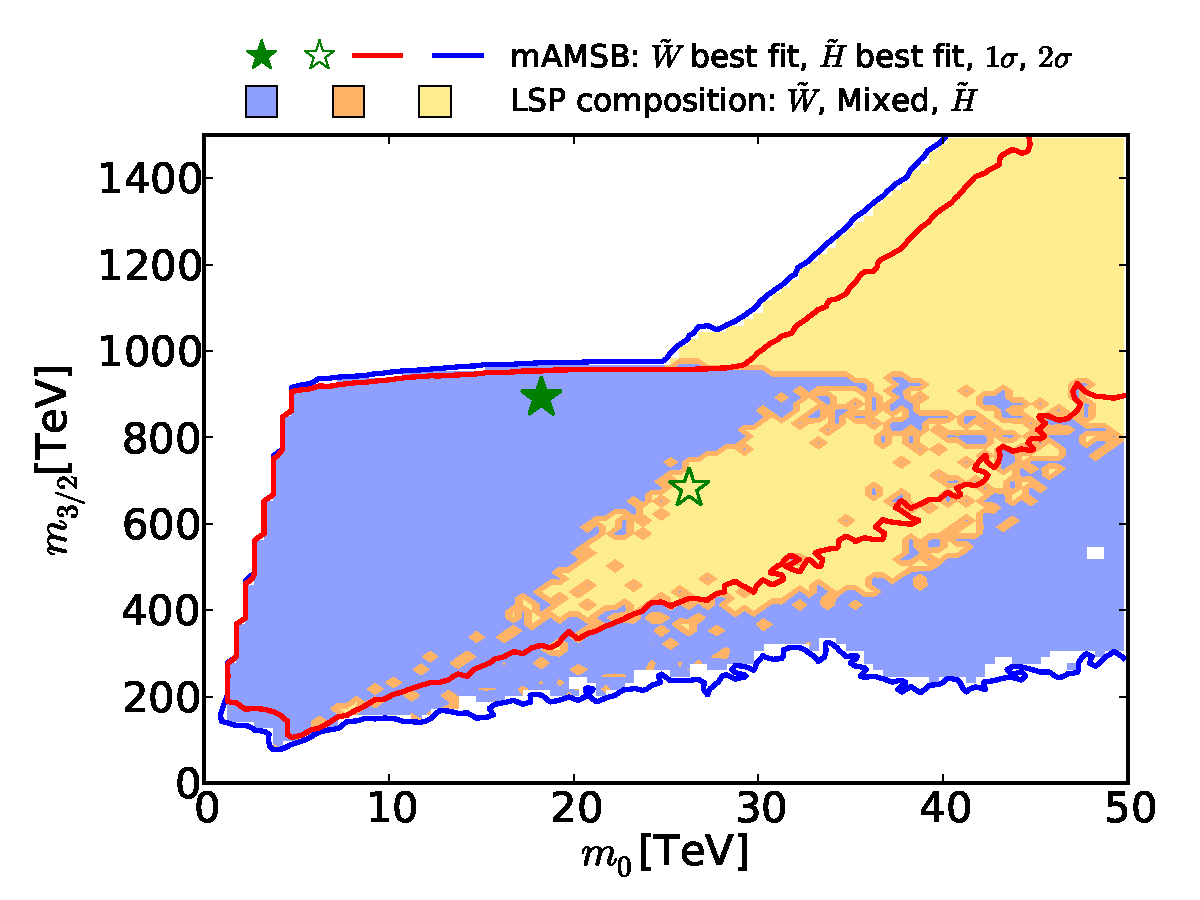
\includegraphics{figs/negmu_noDM_m0TeV50_m32TeV1500_chi2.pdf}}\put(-169, +123){\footnotesize$\mu<0$, $\Omega_{\tilde{\chi}_1^0}<\Omega_{\rm CDM}$}%top left
%\vspace{-3mm}
%\resizebox{7.5cm}{!}{\includegraphics{posmu_noDM_tanb_m32TeV1500_chi2.pdf}}\put(-95, +123){\footnotesize$\mu>0$, $\Omega_{\neu1}<\Omega_{\rm CDM}$}%top right
%\resizebox{7.5cm}{!}{\includegraphics{negmu_noDM_tanb_m32TeV1500_chi2.pdf}}\put(-95, +123){\footnotesize$\mu<0$, $\Omega_{\neu1}<\Omega_{\rm CDM}$}%top right
\end{center}
\vspace{-1.0cm}
\caption{The $(m_0, m_{3/2})$ planes for $\mu > 0$ (left panel) and for $\mu < 0$ (right panel), allowing the $\tilde{\chi}_1^0$ to contribute only part of the CDM density. The best-fit points for the two signs of $\mu$ are indicated by green stars, closed in the
wino-like region and open in the Higgsino-like region.}
%{The shadings are the same as in Fig.~\protect\ref{fig:m0m32}.}}}
\label{fig:m0m32UL}
\end{figure}

Fig \ref{fig:DMdirect_ul} displays the cross section for spin-independent scattering on a proton, $\sigma_p^{\rm SI})$ , versus the neutralino mass, for the case in which the LSP is allowed to contribute only a fraction of the CDM density. As previously, the left plane is for $\mu > 0$, the right plane is for $\mu < 0$, the 1 and 2\,$\sigma$ CL contours are shown as red and blue lines,
and the wino- and Higgsino-LSP regions are shaded in pale blue and yellow. The pale-green-shaded  region represents the range of $\sigma_p^{\rm SI})$\ excluded at the 95\% CL by {a} combination of the latest PandaX and LUX results~\cite{pandax,lux16}, while the purple and {blue} line{s} show the prospective sensitivities of the LUX-Zeplin (LZ), XENON1T {and XENONnT} experiment{s}~\cite{LZ,XENON1T}. Also shown, as a dashed orange line, is the neutrino `floor', below which astrophysical neutrino 
backgrounds would dominate any DM signal~\cite{Snowmass} {(grey region)}. The plot shows good prospects for future DM direct detection experiments when $\mu > 0$, with only a small fraction of the parameter space lying below the neutrino `floor'. {However, when $\mu < 0$ $\sigma_p^{\rm SI})$\ may fall considerably below the `floor', because of cancellations~\cite{cancellations} in the scattering matrix element.}

\begin{figure}[htb!]
\vspace{0.5cm}
\begin{center}
\resizebox{7.5cm}{!}{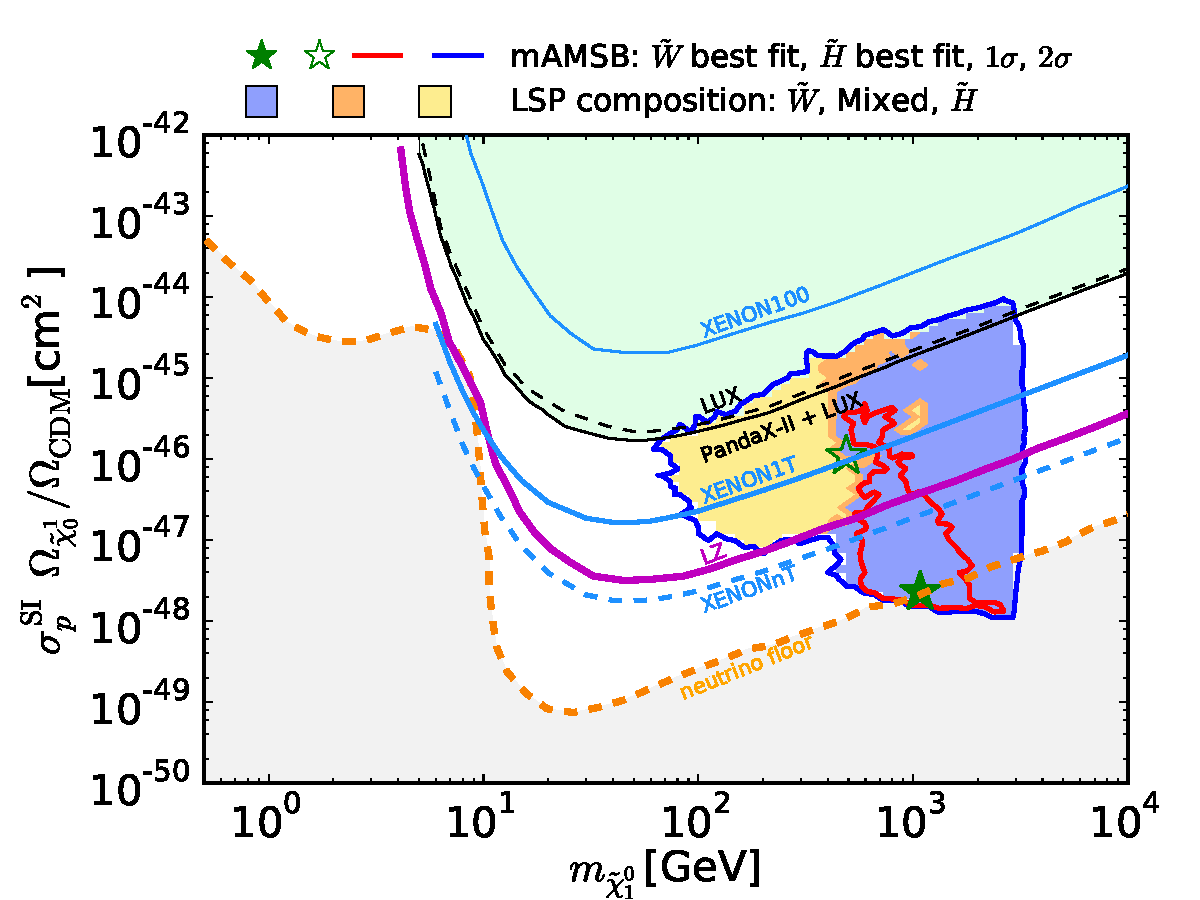
\includegraphics{figs/posmu_noDM_logabsmneu1_SNOW_logssikocm2_SNOW_oh2scaled_chi2.pdf}}\put(-95, +123){\footnotesize $\mu>0$, $\Omega_{\tilde{\chi}_1^0}<\Omega_{\rm CDM}$}%top right
\resizebox{7.5cm}{!}{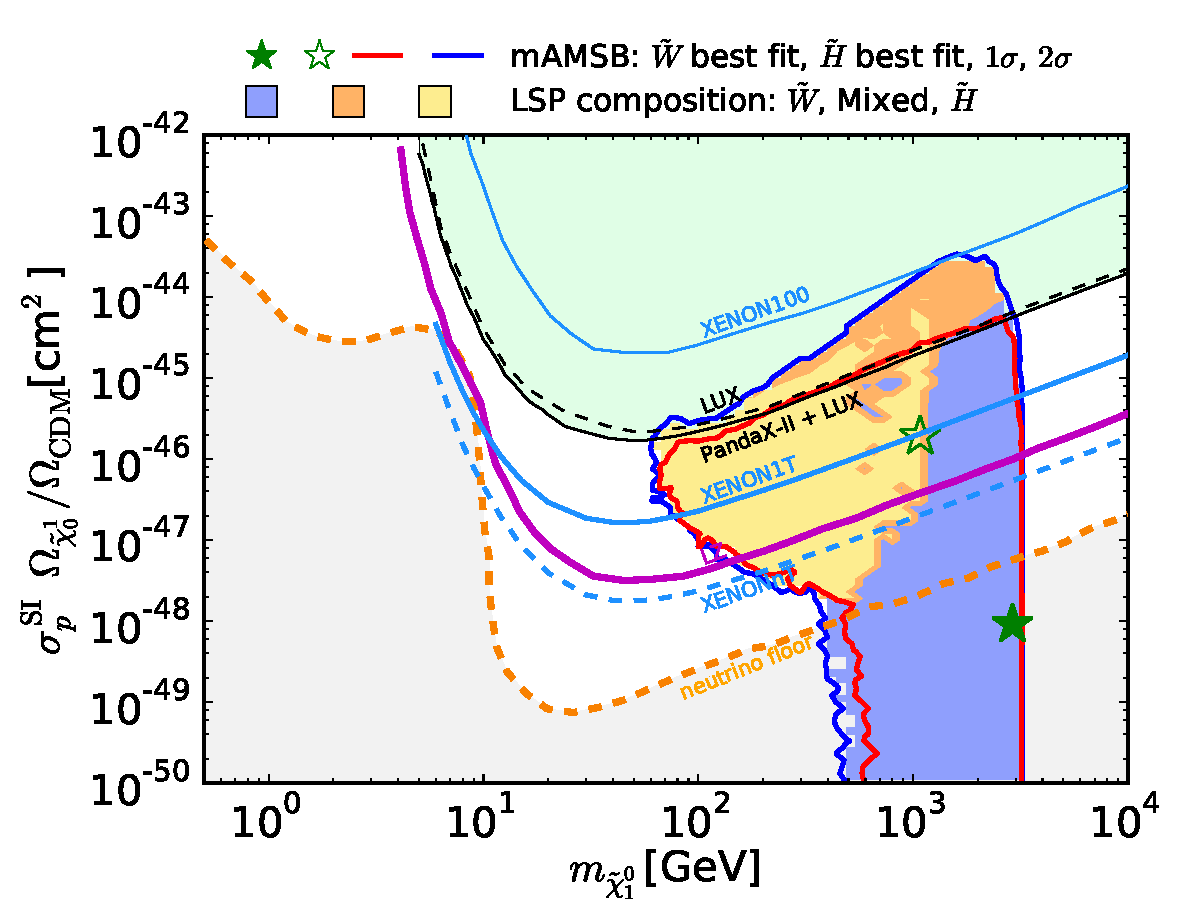
\includegraphics{figs/negmu_noDM_logabsmneu1_SNOW_logssikocm2_SNOW_oh2scaled_chi2.pdf}}\put(-95, +123){\footnotesize $\mu<0$, $\Omega_{\tilde{\chi}_1^0}<\Omega_{\rm CDM}$}%top right
\end{center}
\caption{The $(m_{\tilde{\chi}_1^0}, \sigma_p^{\rm SI})$ planes in the mAMSB for $\mu>0$ (left)
and $\mu<0$ (right) in the case when the LSP only accounts for a fraction of the CDM density. 
The best-fit points for the two signs of $\mu$ are indicated by green stars, closed in the
wino-like region and open in the Higgsino-like region.}
\label{fig:DMdirect_ul}
\end{figure}
%%% the renormaliztion group equations exhibit a novel "focus point" (as opposed to fixed point) behavior, which allows squark and slepton masses far above theirusual naturarlness bounds
%%% anomaly-mediated SUSY breaking parameters 
%%% the susy breaking parameters are then evolved with one-loop RG equations to the superparticle mass scale, m_SUSY
%%% beta functions in hep-ph/9907319v1
%%% mAMSB: ew symmmetry is broken raditively due to the large top quark mass
%%% GUT scale boundary conditions

\begin{comment}
two neutralino states with defined masses
supergravity?
check consistency in notation
https://arxiv.org/pdf/hep-ph/9907319.pdf
https://arxiv.org/pdf/hep-ph/0006049.pdflllllll
https://arxiv.org/pdf/hep-ph/0101034.pdf
https://arxiv.org/pdf/1004.3297.pdf

%%% UN CONHAZO:
https://arxiv.org/pdf/hep-th/9810155.pdf %%% the very worst
https://arxiv.org/pdf/hep-ph/9904378.pdf
https://arxiv.org/pdf/hep-ph/9909376.pdf
\end{comment}


\subsection{Renormalization Group equations}
\label{sec:renormalization}
%%%% arXiv:hep-ph/9709356v7

%%Objetivo 
The renormalization grop equations(RGE) are applied within the MSSM to describe the evolution of gauge couplings, superpotential parameters and soft terms from a given \textit{input} scale up to near the \textit{electroweak} scale. The method used in the SM (dimensional regularization, DREG) cannot be used within SUSY, as it introduces a spurious violation of this symmetry. The most common method for it is the dimensional reduction, DRED, with modified minimal subtraction ($\rm \overline{DR}$), as opposed to DREG with modified minimal subtraction ($\rm \overline{MS}$). 
%% the boundary conditions at the input scale should presumably be applied in a supersymmetry-preerving scheme like DR
Figure \ref{fig:RGE} compares the RG evolution of the coupling constants both in the SM and in the MSSM. As it can be seen, a better match at the electroweak scale is achieved within the MSSM, as discussed in \ref{sec:introduction}. 

\begin{figure}[htb!]
\begin{center}
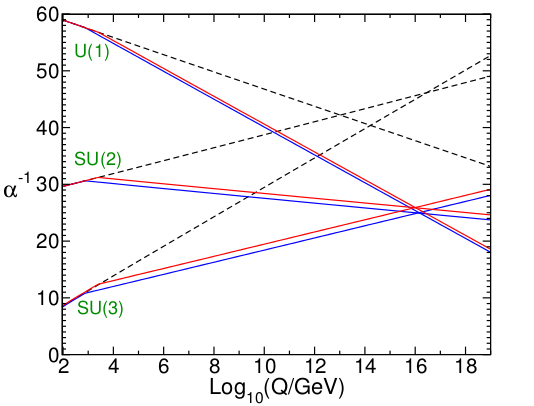
\includegraphics[scale=0.6]{figs/RGE.png}
\end{center}
\caption{Two-loop renormalization group evolution of the inverse gauge couplings $\alpha_a^{-1}(Q)$ in the SM (dashed lines) and the MSSM (solid lines). In the MSSM case, the sparticle masses are treated as a common threshold varied between 750 $\rm GeV$ and 2.5 $\rm TeV$, and $\alpha_3(m_Z)$ is varied between 0.117 and 0.120~\cite{Martin:1997ns}.}
\label{fig:RGE}
\end{figure}

The RGE are derived using what is known as the \textit{supersymmetryc non-renormalization theorem}, that implies that the logarithmically divergent contribution to a particular process can always be written in terms of wave-function renormalizations\red{~\cite{Martin:1997ns}}. One consequence derived from this is that for a given value of $\mu$ \red{at tree-level}, RG corrections to it will be proportional to the parameter itself and some combinations of dimensionless couplings, thus avoiding very large radiative corrections that could greatly enhance $\mu$. 

Within this framework, it is asumed that gauge couplings unify at a given scale, $\Lambda$. Hence, gaugino masses are considered to be unified near that scale as well (which come naturally in GUT models):
\begin{equation}
\frac{M_1}{g_1^2} = \frac{M_2}{g_2^2} = \frac{M_3}{g_3^2} = \frac{m_{1/2}}{g_{\Lambda}^2}
\end{equation}

where $g_\Lambda$ is the unified gauge coupling at $\Lambda$, and $m_{1/2}$ the unification value for the gaugino masses.

%%Consecuencias
Some more consequences of the RGE are listed below. 

\begin{enumerate}
\item Because they are not protected by the supersymmetric non-renormalization theorem, the soft parameters that describe the Yukawa couplings don't vanish at the electroweak scale, even if they are zero at the input scale. %%% not protected by the supersymmetryc non-renormalization
\item The scalar squared masses will be almost diagonal, with the second family squarks and sleptons very nearly degenerate. The third-family squarks and sleptons will get normalized differently 
\item The scalar squared-mass parameters grow as they are RG-evolved, due to the gaugino masses effect on the RGE. Therefore, large masses can be obtained at the electroweak scale even if these are small or even zero at the weak scale. 
\item Because of the contributions they receive from the RGE, the Higgs squared masses generally decrease at the electroweak scale with respect to the input scale. This can lead to a negative value of $m_{H_u}^2$, with the consequence of a non-zero Higgs vev. This effect increases as the top Yukawa coupling does. %%% Thus a large top Yukawa coupling favors the breakdown of the electroweak symmetry breaking because it induces negative radiative corrections to the Higgs squared mass. These facts make it plausible that the Higgs scalars in the MSSM get VEVs, while the squarks and sleptons, having large positive squared mass, do not.
\item If the gaugino mass parameters $M_1$, $M_2$ and $M_3$ have non-zero values for a given input scale, all the soft terms will be generated via RGE. Otherwise, gauginos would be extremely light, causing the model to be inviable due to experimental measurements.%%This implies that models in which gaugino masses dominate over all other effects in the soft supersymmetry breaking Lagrangian at the input scale can be viable.
\end{enumerate}

\section{RPV Models}
\label{sec:RPV}
%%% arXiv:hep-ph/9709356v7
%%% arXiv:1401.7989v4
%%% 
R-parity (or matter parity) conservation can be justified in terms of a grand unified theory or as a consequence of a residual symmetry of a superstring vacuum. However, it is not necessarily the existing scenario. Additional terms can be added to the superpotential in \ref{eq:superpotential} that violate baryon number (B) or lepton number (L), namely: \red{check consistency with other equation}
\begin{equation}
W_{\Delta L=1} = \frac{1}{2}\lambda^{ijk}L_iL_j\overline{e}_k + \lambda'^{ijk}L_iQ_j\overline{d}_k + \mu'^i L_i H_u 
\label{eq:DL}
\end{equation}
\begin{equation}
W_{\Delta B=1} = \frac{1}{2}\lambda''^{ijk}\overline{u}_i\overline{d}_j\overline{d}_k
\label{eq:DB}
\end{equation}
Where $i=1,2,3$, depending on the fermionic family. Terms in \ref{eq:DL} (\ref{eq:BL}) violate lepton (baryon) number by 1 unit. If both terms accompanying $\lambda'$ and $\lambda''$ were to exist (without suppression), proton decays to final products such as $e^+\pi^0$ would be feasible. Nevertheless, the lifetime for the proton is known to be $> 10^{34}$ years\red{~\cite{Nishino:2009aa}}. This, together with more experimental evidence , leads to the conclusion that one of these couplings must be zero or very small, being RPV models either B-violating or L-violating, with experimental upper bounds existing for both couplings. 

One example of such type of RPV model is a scenario where R-parity is replaced by a \textit{baryon triality}, defined in \ref{eq:triality}.
\begin{equation}
Z_3^B = \exp{2\pi i[B-2Y]/3}
\label{eq:triality}
\end{equation}
The corresponding symmetry establishes that the product of the baryon trialities of the particles in any term in the superpotential must be 1. With this, proton decay and neutron-antineutron oscillation are forbidden processes, as they would violate triality. This symmetry does allow the LSP to decay. 

Another alternative is the spontaneous R-parity symmetry breaking by particles, like sneutrinos in the context of MSSM(~\cite{MASIERO1990273},~\cite{ROMAO1992311}). Strong experimental bounds exist on this\red{ref?}. Either way, RPV scenarios greatly change the SUSY signatures in colliders, allowing processes like single sfermion production or exchange of sfermions to happen. %% \red{ref,A. Masiero and J.W.F. Valle, Phys. Lett. B 251, 273 (1990); J.C. Romao, C.A. Santos and J.W.F. Valle, Phys. Lett. B 288, 311 (1992)}

\subsection{Consequences of RPV}
\label{sec:RPVcons}
Numerous consequences can be derived in the different possible RPV models. Some of them are briefly addressed below. 
\begin{enumerate}
\item Within some of these models, there can be \textit{leptogenesis} (asymmetry between leptons and antileptons in the early Universe), that would lead to the current matter-antimatter asymmetry discussed in \ref{sec:introduction}.
\item The LSP can have color/charge, while fulfilling current constraints, and no longer needs to be stable. 
\item Some RPV models include a seesaw mechanism that provides neutrinos with mass, while including sterile neutrinos~\cite{Ghosh:2010hy}.
\item A possible candidate for DM is the heavy gravitino, superpartner of the graviton. Even though it is unstable, its decay is heavily suppressed by the gravitational coupling, resulting in a lifetime bigger than the age of the Universe. 
\end{enumerate}

%%\red{numbers for RP for gauge bosons and gauginos, N=1 SUSY}
%%%% description (marron)
%%%% advantages and disadvantages (red)
%%%% examples (blue)
%%%% experimental signatures (atlas status) 

\section{Experimental searches}
\label{SUSY:exp}

Many experimental efforts have been done in the search for supersymmetry, both via direct searches of supersymmetric particles and by looking for indirect effects. A summary of the former is represented in figures \ref{fig:ATLASSUSYexp} and \ref{fig:CMSSUSYexp}, where bounds on the masses are set for different models, with data from ATLAS and CMS experiments, described in chapter \ref{chap:LHCb}.  

With these experimental constraints, together with other experimental measurements, such as DM direct detection results \ref{} global fits can be made for different SUSY models. A specific case will be discussed in chapter \ref{chap:CMSSM}. More of these fits can be found in~\cite{Athron:2018vxy},~\cite{Athron:2017yua},~\cite{Athron:2017qdc},~\cite{Bagnaschi:2016afc},  
~\cite{Bagnaschi:2016xfg},~\cite{Bagnaschi:2017tru},~\cite{Costa:2017gup}.

\begin{figure} [htb!]
\begin{center}
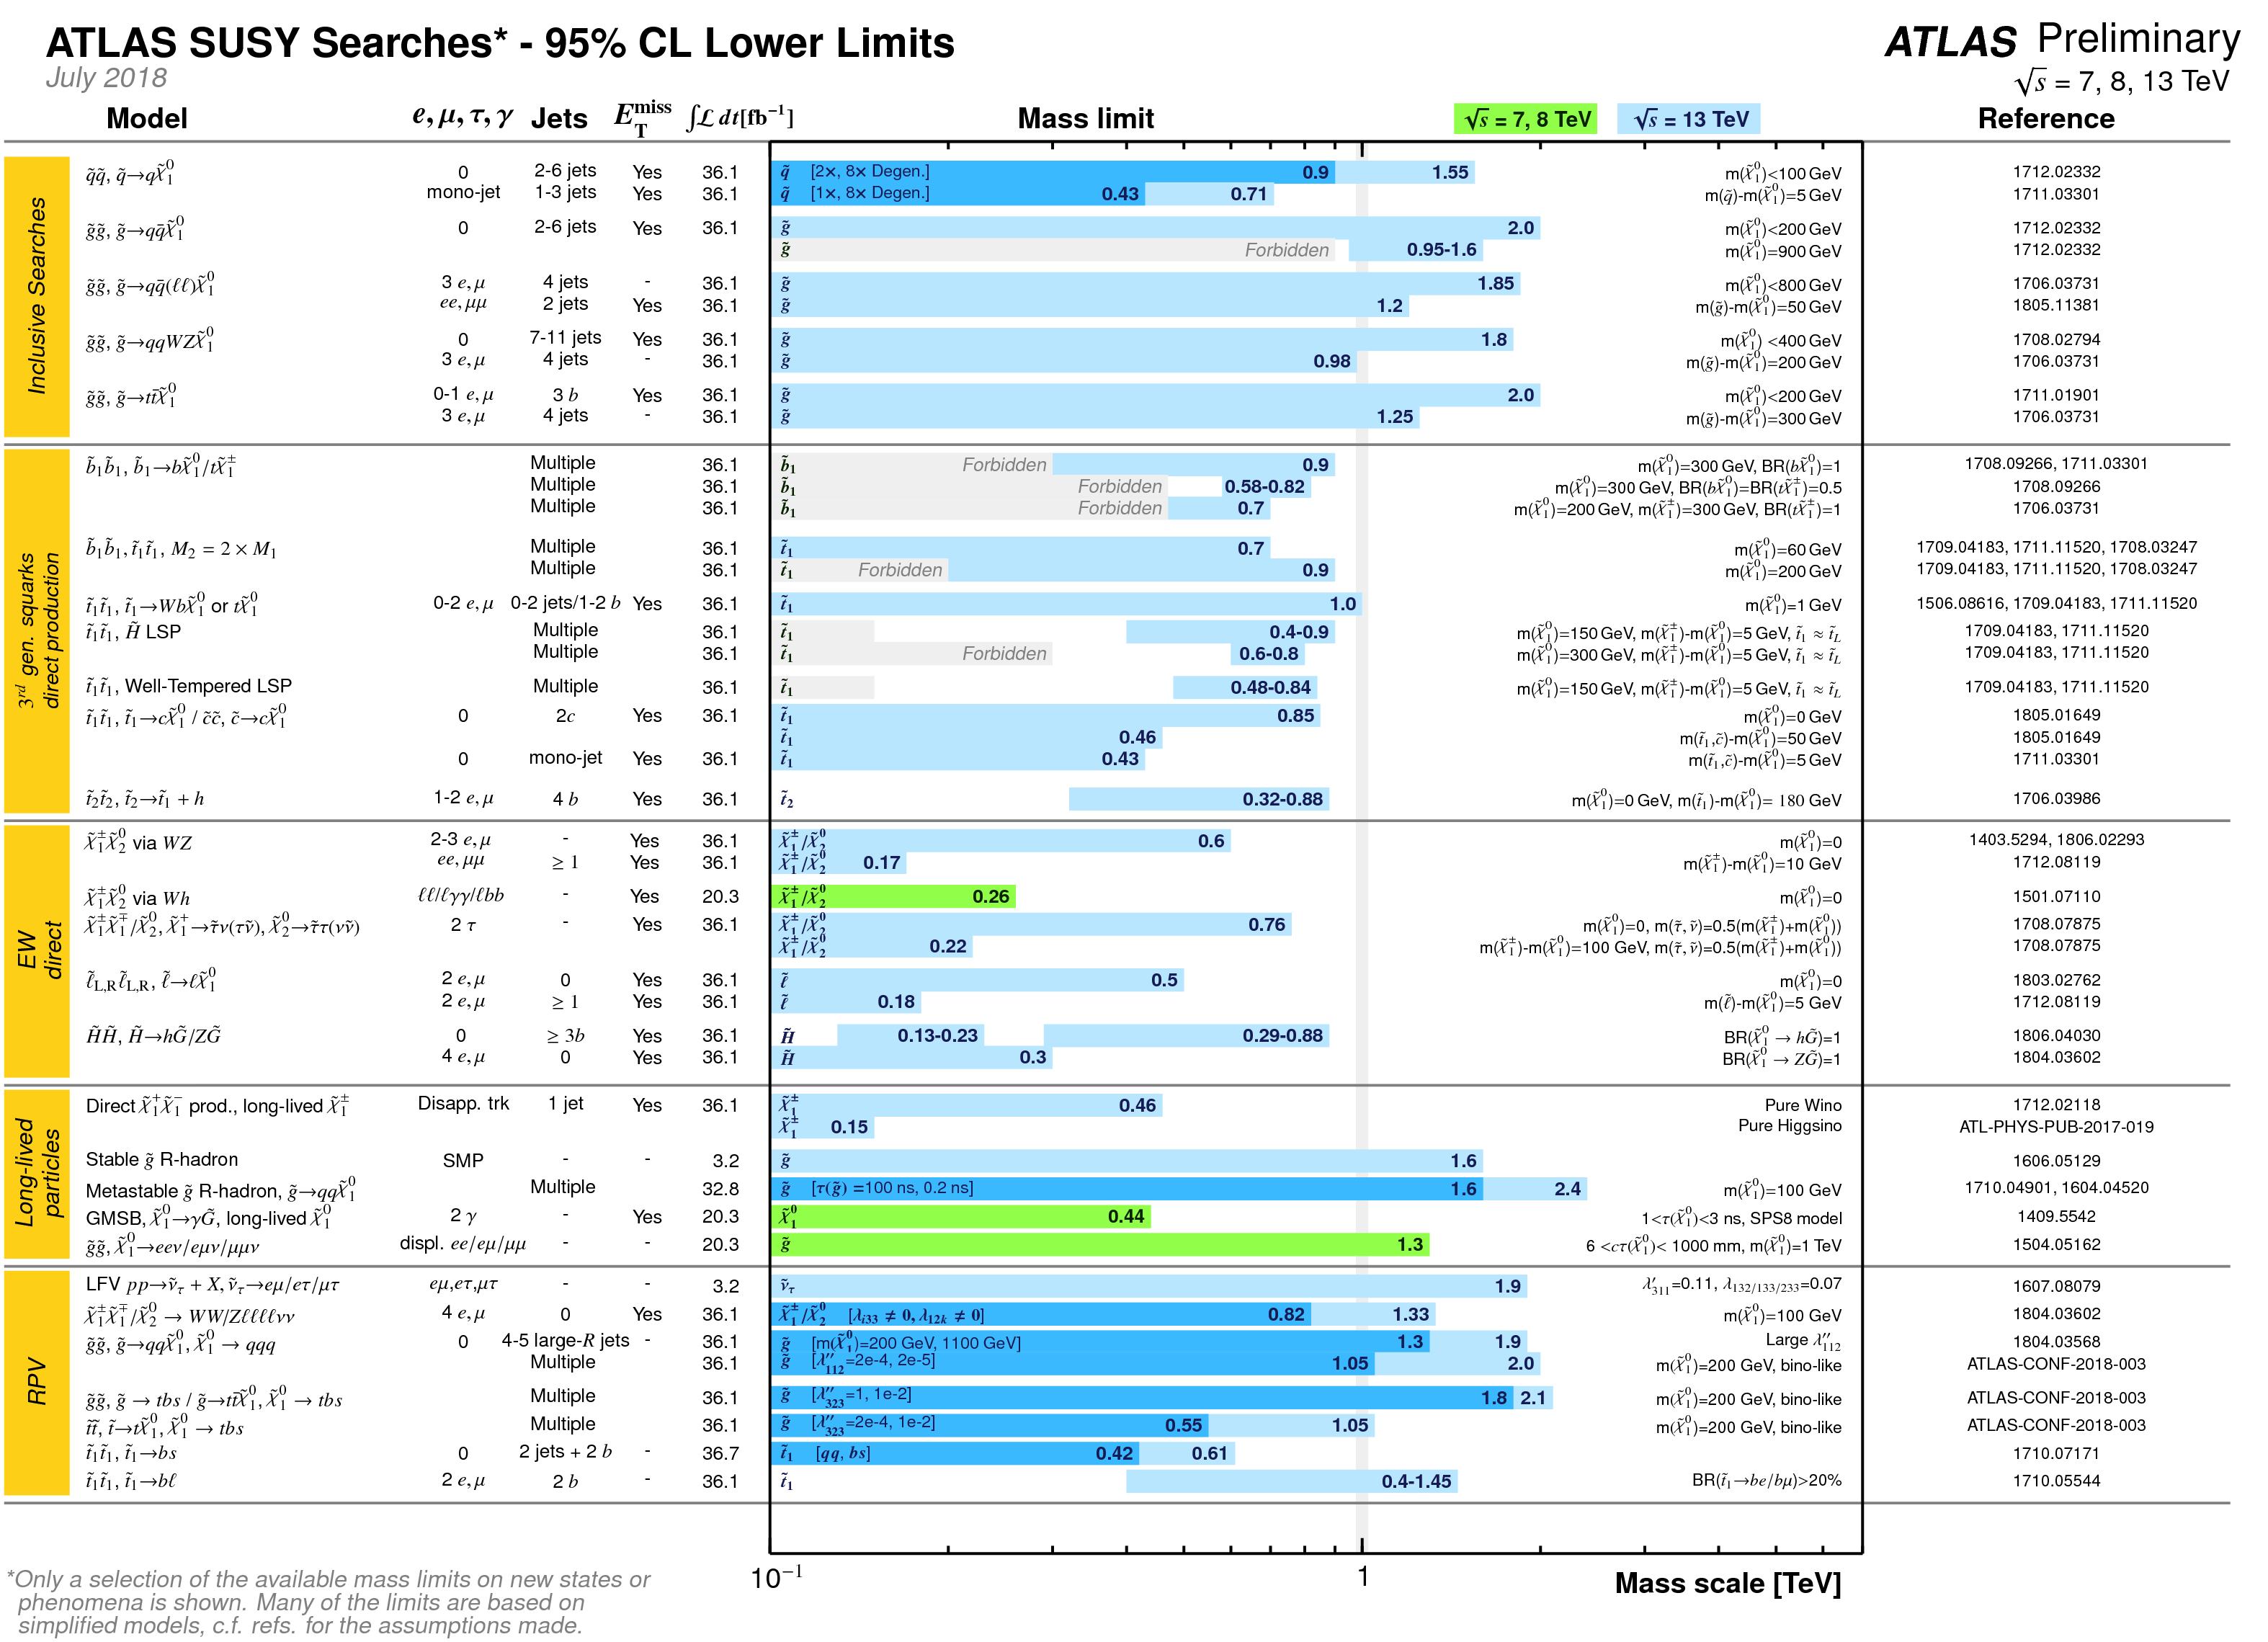
\includegraphics[scale=0.15]{figs/ATLAS_SUSY_Summary.png}
\caption{Experimental status of SUSY searches in ATLAS\label{fig:ATLASSUSYexp} \red{ref}}
\end{center}
\end{figure}

\begin{figure} [htb!]
\begin{center}
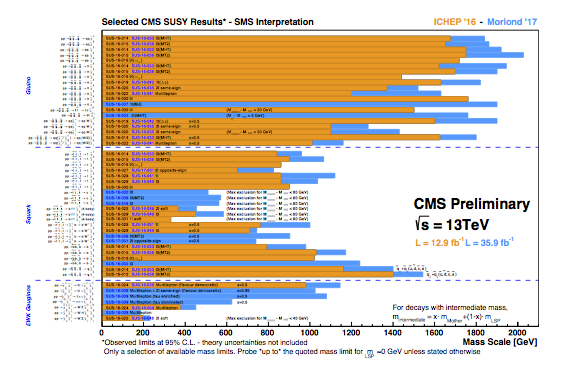
\includegraphics[scale=0.70]{figs/CMS_SUSY_Summary.png}
\caption{Experimental status of SUSY searches at CMS\label{fig:CMSSUSYexp} \red{ref}}
\end{center}
\end{figure}


 
\chapter{Low E in SUSY (MFV)}
\label{sec:SUSY}


%%% definition - maroon
%%% motivation - blue
%%% characteristics - red
%%% other models (CMFV) - violet
%%% experimental bounds and signatures - pink
%%% EFT

\section{Motivation for MFV}
\label{sec:MFVMot}
The succes of the SM in predicting flavour and CP violation effects leads to thinking that NP has to follow its pattern. Otherwise, experimental evidence of additional flavour violting structures should have appeared by now. Additionally, the hierarchy problem suggests $\Lambda < \rm TeV$, while in the case in which flavour violation is generated generically in SUSY, $\Lambda \sim \mathcal{O}(\rm TeV)$~\cite{Paradisi:2009ey}. 
An effective field theory (henceforth, EFT) becomes necessary in order to address the favour problem in SUSY, where the flavour violation predictions can largely exceed the experimental constraints and are \textit{a priori} unrelated to the SM sources ~\cite{Altmannshofer:2007cs}. 
 %%% SUSY CP problem 
%\section{MFV}
%\label{sec:MFVdesc}
Minimal Flavour Violation (hereafter MFV) requires all flavour and CP-violating interactions to be governed by the known structure of the SM Yukawa couplings~\cite{DAmbrosio:2002vsn} in the low-energy regime. Hence, in any SM extension the amount of FCNC and CP violating process should be ruled by these.  
As for supersymmetry, MFV holds under the assumption of \textit{mass universality}, and if the trilinear soft terms are proportional to the Yukawa couplings at the GUT scale. 
This MFV can be seen as the remnant of an underlying favor symmetry at the $\Lambda$ scale~\cite{Paradisi:2009ey}. 

\section{MFV EFT}
\label{sec:MFVEFT}
Minimal Flavour Violation (hereafter MFV) is constructed as a low-energy EFT~\cite{DAmbrosio:2002vsn}, within which the SM is contained. Its main feature is that the only source of $SU(3)^5$ flavour symmetry breaking are the background values of fields transforming under the flavour group like the ordinary Yukawa couplings~\cite{DAmbrosio:2002vsn}. 
In he SM, the $U(3)^5$ flavour symmetry is the largest group of unitary field transformations that commutes with the gauge group. This can be decomposted~\cite{DAmbrosio:2002vsn} as:
\red{$U(3)^5 = [SU(3)]^5 \bigotimes U(1)_E5$, more details}
%\begin{equation}
%G_F \equiv SU(3)_q^3 \bigotimes SU(3)_l^3 \bigotimes U(1)_B \bigotimes U(1)_B \bigotimes U(1)_L \bigotimes U(1)_Y \bigotimes U(1)_{PQ} \bigotimes U(1)_{E_R}
%\end{equation}
%where
%\begin{equation}
%SU(3)_q^3 = SU(3)_{Q_L} \bigotimes SU(3)_{U_R} \bigotimes SU(3)_{D_R} \ \
%SU(3)_l^2 = SU(3)_{L_L} \bigotimes SU(3)_{E_R}
%\end{equation}
\begin{equation}
%G_F \equiv \bigotimes [SU(3) \bigotimes U(1)]_F, \ F=Q,U,D,L,E
\end{equation}
Notice that the baryon, lepton and hypercharge numbersare not modified by Yukawa interactions. %The remaining U(1) groups correspond to the Peccei-Quinn symmetry of THDM \red{ref} and a global rotation of a single $SU(2)_L$ singlet. %%rearranged (MFV_TOTAL)
The $U(3)^5 = [SU(3) \bigotimes U(1)]^5$ \red{check} group is broken by Yukawa interactions. Flavour invariance is recovered introducing dimensionless auxiliary fields, $Y_U$, $Y_D$ and $Y_E$ transforming under $SU(3)_q^3 \bigotimes SU(3)_l^3$ promoting to \red{spurion} fields in order for flavour violation to appear ~\cite{Altmannshofer:2007cs}, thus leading to the Yukawa interaction terms of the SM lagrangian \red{as discussed in \ref{sec:introduction}}, consistent with flavour symmetry. These term can be rotated such that: %%%% Responsible for such breaking are the SM Yukawa couplings, and their transformation properties under the flavour group can be identified by requiring (formal) invariance of the Yukawa interactions. FV is recovered as the spurion Yukawa 'fields' assume their bkg values. MFV then demands the Yukawa bkg values to be the only structures generating the observed flavour (and CP) violation

%%% spurions == small (Grossman)
\begin{equation}
Y_d = \hat{Y}_d, \ Y_e = \hat{Y}_e, \ Y_u = V^{\dagger}\hat{Y}_u
\end{equation}
denoting $\hat{Y}$ diagonal matrices, and $V$ being the CKM matrix. The notation in ~\cite{DAmbrosio:2002vsn} is followed.  

In MFV all higher-dimensional operators are constructed from SM and $Y$ fields, and are invariant under CP and the flavour group $G_F$. Therefore, they can be rewritten in terms of the SM Yukawa couplings ~\cite{Altmannshofer:2007cs}. Given that the top Yukawa coupling is considerably large with respect to the others, the only relevant non-diagonal structure \red{in the low $\tan{\beta}$ regime} is obtained contracting two $Y_u$, hence having:
\begin{equation}
\left(\lambda_{FC}\right)_{ij} = \left\{\begin{matrix}
\left( Y_u Y_u^{\dagger} \right)_{ij} \approx \lambda_t^2 V_{3i}^* V_{3j} & i \neq h\\ 
0 & i = j 
\end{matrix}\right.
\label{eq:lambda}
\end{equation}
where $\lambda_t = (\hat{Y}_u)_{33}$ and subleading effects on the r.h.s of \ref{eq:lambda} are suppressed by powers of $m_c/m_t$~\cite{Altmannshofer:2007cs} as the effective coupling ruling all FCNC processes with external down-type quarks. Such processes are governed by $\Delta F = 2$ and $\Delta F = 1$ (Higgs field, gauge fields and four-fermion) operators. Further details on this operators can be found in ~\cite{DAmbrosio:2002vsn}. 

%%% Left out from MFV_TOTAL: dimension-six operators 


\section{MFV SUSY}
\label{sec:MFVSUSY}
Consider the MSSM (where R-parity is conserved) as a low-energy EFT. Differently to what happens in other non-supersymmetric MFV scenarios, there are renormalizable terms with non-trivial flavour structure, besides the ordinary Yukawa couplings.
Within MFV, the off-diagonal entries in the soft terms (the genuinely new sources of flavour violation in the MSSM) are CKM-like~\cite{Altmannshofer:2007cs}.

The squark mass matrices after the electroweak breaking and using the soft terms, \ref{eq:soft4} and \ref{eq:soft5} have the form 

\begin{equation}
\tilde{M}_U^2 = 
\left( \begin{matrix}
\tilde{m}_{Q_L}^2 + Y_uY_u^{\dagger}v_u^2 + (1/2 - 2/3\sin{\theta_W}^2)M_Z^2\cos{2\beta} & (A_u - \mu Y_u\cot{\beta})v_u \\
(A_u - \mu Y_u\cot{\beta})^{\dagger}v_u & \tilde{m}_{U_R}^2 + Y_U^{\dagger}Y_uv_u^2 + 2/3\sin{\theta_W}^2M_Z^2\cos{2\beta} \\
\end{matrix}\right)
\label{eq:MU}
\end{equation}

\begin{equation}
\tilde{M}_D^2 = 
\left( \begin{matrix}
\tilde{m}_{Q_L}^2 + Y_dY_d^{\dagger}v_d^2 + (1/2 - 1/3\sin{\theta_W}^2)M_Z^2\cos{2\beta} & (A_D - \mu Y_d\tan{\beta})v_d \\
(A_d - \mu Y_d\tan{\beta})^{\dagger}v_D & \tilde{m}_{D_R}^2 + Y_D^{\dagger}Y_dv_d^2 - 1/3\sin{\theta_W}^2M_Z^2\cos{2\beta} \\
\end{matrix}\right)
\label{eq:MD}
\end{equation}

According to MFV, the squark masses and trilinear couplings in \ref{eq:MU},\ref{eq:MD} can be written as follows~\cite{DAmbrosio:2002vsn}:
\begin{equation}
\tilde{m}_{Q_L}^2 = \tilde{m}^2(a_1\mathbb{I} + b_1Y_uY_u^{\dagger} + b_2Y_dY_d^{\dagger} + b_3Y_dY_d^{\dagger}Y_uY_u^{\dagger} + b_4Y_uY_u^{\dagger}Y_dY_d^{\dagger})
\label{eq:soft1}
\end{equation}
\begin{equation}
\tilde{m}_{U_R}^2 = \tilde{m}^2(a_2\mathbb{I} + b_5Y_uY_u^{\dagger})
\label{eq:soft2}
\end{equation}
\begin{equation}
\tilde{m}_{D_R}^2 = \tilde{m}^2(a_3\mathbb{I} + b_6Y_dY_d^{\dagger})
\label{eq:soft3}
\end{equation}
\begin{equation}
A_U = A(a_4\mathbb{I} + b_7Y_dY_d^{\dagger})Y_u
\label{eq:soft4}
\end{equation}
\begin{equation}
A_D = A(a_5\mathbb{I} + b_8Y_uY_u^{\dagger})Y_d
\label{eq:soft5}
\end{equation}
Where $\tilde{m}$ and A set the mass scale of the soft terms, $a_i$ and $b_i$ are numerical coefficients and $\mathbb{I}$ is the 3x3 identity matrix. Quadratic terms of the first two families of Yukawas have been neglected. In the limit of low $\tan{\beta}$ the terms quadratic in $Y_d$ can be dropped too.%%% kept independent flavour structures proportional to third-generation Yukawa coplings 

Under the assumption of mass universality and proportionality of trilinear terms, the $b_i$ coefficients are zero at the GUT scale $\Lambda$ and generated via RGE. %%% also by integrating out heavy state at the cut-off scale Lambda  (MFV_TOTAL)

It is worth noticing from \ref{eq:MU}, \ref{eq:MD} the physical squark masses are not degenerate under the MFV assumption, but the mass splitting is severely constrained. 

The mass matrices in \ref{eq:MD} and \ref{eq:MU} are then diagonalized using the expansions in \ref{eq:soft1},\ref{eq:soft2},\ref{eq:soft3},\ref{eq:soft4} and \ref{eq:soft5}. Analogously to the SM case, it is possible to change to a \textit{super-CKM} basis, where:

\begin{equation}
\hat{m}_u = \frac{v_d}{\sqrt{2}}\hat{Y}_{u},\ \hat{m}_d = -\frac{v_u}{\sqrt{2}}\hat{Y}_{d}
\end{equation}

Notice that in this basis the Yukawa matrices are diagonal, but the trilinear coplings and the mass-matrices are still non-diagonal. Unitary matrices $Z_U$ and $Z_D$ are needed in order to change to a mass eigenstate basis. In the MFV scenario the off-diagonal entries of this matrices are not zero, but CKM-like ~\cite{Altmannshofer:2007cs}.

\red{equation?, MIA?}

\section{MFV R-parity}
\label{sec:MFVRPV}
MFV can be used instead of the R-parity conservation assumption ~\cite{Csaki:2011ge}. Under this scenario the baryon number can be violated, while the lepton number violation is strongly suppressed and only possible with massive neutrinos. \red{This is strongly discouraged by the proton lifetime, and bounds from $n - \bar{n}$ oscillation and dinucleon decay.} In some specific models, extra suppression from the neutrino sector can help further alleviate this bounds. 
Under this models \red{R-parity is obtained as an approximate symmetry as a side effect}. The LSP decays fast and is not necessarily neutral, it can be a stop or sbottom (decaying to 2 bodies), a neutralino or chargino (decaying to 3 bodies) or a slepton (with the subsequent 4 body decay). A possible DM candidate is the gravitino. 

%\section{MFV EW scale}
%\label{sec:MFVEW}

%\section{MFV GUT scale}
%\label{sec:MFVGUT}

\section{Characteristics}
\label{sec:MFVChar}
Given that the top Yukawa coupling is much larger than the others, in MFV all flavour-changing effective operators are proportional to the same non-diagonal structure. This greatly affects the \red{predictability} of this model, as will be discussed in \ref{sec:MFVExp}. 
Within this approach, the squark masses in the physical eigenbasis are not deenerate, but the induced flavour violation is described in ters of the usual CKM parameters~\cite{DAmbrosio:2002vsn}. 

Strong assumptions need to be made in order to maintain MFV within different SUSY scenarios, such as supergravity. Other models with different susy-breaking mechanism (such as AMSB) can alleviate this \red{conundrum} ~\cite{DAmbrosio:2002vsn}.

As will be discussed in \ref{sec:UT}, the Universal Unitarity Triangle does not necessarily hold within the MFV scenario. 

Within MFV, both the gaugino masses $M_{1,2}$ and the Higgs mixing parameter $\mu$. Otherwise, given that they appear in the neutralino and chargino mixing matrices, they would induce new sources of CP violation, thus violating MFV. An \red{alternative} approach ~\cite{Straub:2009jd} consists \red{in} assuming the soft SUSY breaking sector to be CP conserving only in the limit of flavour blindness, while allowing CP violation to happen by the MFV-compatible terms. In this scenario, $\mu$ and the gaugino masses are real at low energies and the trilinear coupings (\red{the only sources of CP-violation}) are strongly hierarchical, being the EDMs \red{explain} the most \red{important} experimental constraints~\cite{Paradisi:2009ey}. Nevertheless, in the case in which this \textit{ansatz} holds not at the low scale, but at the GUT scale (determined by $\Lambda$), complex parameters can be generated via RGE~\cite{Paradisi:2009ey},~\cite{Straub:2009jd}.
\section{CMFV}
\label{sec:CMFV}
The \textit{constrained} MFV (cMFV) is a phenomenological definition of MFV, that uses the CKM matrix (instead of the Yukawa couplings) as the only source of flavour violation and retricts the set of relevant operators in the low-energy effective Hamiltonian to the SM ones ~\cite{Altmannshofer:2007cs} ($\mathcal{Q}_1$).%%% CMFV
Contrarily to the more general definition of MFV proposed in ~\cite{DAmbrosio:2002vsn}, it is not model-independent. In the limit in which $b_i \rightarrow 0$ in \ref{eq:soft1}-\ref{eq:soft5}, the cMFV is recovered from the general MFV. Nevertheless, it is worth mentioning that not all the scenarios are $\mathcal{Q}_1$-dominated, as it is assumed in cMFV. Indeed, in the limit of low $\tan{\beta}$ it is not always the case ~\cite{Altmannshofer:2007cs}. 


\section{Experimental bounds}
\label{sec:MFVExp}
Generic flavour-violating interactions at $\Lambda \simeq \rm TeV$ are known to be experimentally excluded. 
Within a MFV scenario, it is possible to \red{relate} various flavour-changing neutral current (FCNC) processes, such as rare $B$ and $K$ decays. Furthermore, CP-violation in the $B_s$ system provide an excellent probe where to look for non-CKM sources of flavour and CP-violation~\cite{Altmannshofer:2007cs}. Besides, this constraint in the soft sector helps further reduce the number of parameters of the MSSM, discused in \red{ref}, thus improving its predictivity. 

Experimental bounds to the generic MFV approach come mainly from:
\begin{itemize}
\item $\Delta F = 2$ processes that help further improve the precision for CKM matrix elements
\item The inclusive rare decay $B \rightarrow X_s \gamma$  to constraint the scale of the FCNC operators \red{check}
\item Rare FCNC decays into a lepton pair, e.g. $K_L(B) \rightarrow l^+ l^-$, $K^+ \rightarrow \pi^+ \nu \bar{\nu}$, that provide constraints on several Wilson coefficients %%% MFV_TOTAL
\item Non-leptonic decays, provided electroweak contributions can be properly disentangled from the dominant effects coming from tree-level and gluon-penguin amplitudes %%% MFV_TOTAL
\end{itemize}

\section{Unitarity Triangle}
\label{sec:UT}

The \textit{universal unitarity triangle}~\cite{Buras:2000dm} (henceforth, UUT) represented in \ref{fig:uut} is characterized by not having any new operators beyond those present in the SM, hence only valid for cMFV models \ref{sec:CMFV}. Depending on the mass regime and the value of $\tan{\beta}$, variations up to the percent level can be found in a general MFV scenario~\cite{Altmannshofer:2007cs}. 
In this triangle, no phases are beyond the CKM phase, hence they are not polluted by new physics contributions (since the quantities only depend on the CKM parameters). \red{A virtue of the universal triangle is that it allows to separate the determination of the CKM parameters from the determination of new parameters present in the extensions of the SM, since new physics could contribute to the values. As an example, new phases could affect $\alpha$, $\beta$ and $\gamma$.} 

\begin{figure} [htb!]
\begin{center}
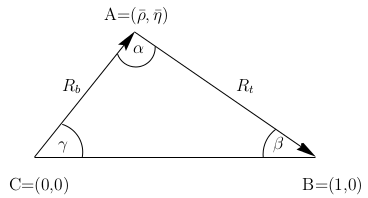
\includegraphics[scale=0.7]{figs/uut.png}
\caption{Unitarity Triangle, using the Wolfenstein parametrization \red{ref, PDG}\label{fig:uut}}
\end{center}
\end{figure}

Experimental measurements help determining the different values for the elements that define the triangle in \ref{fig:uut}. Some of these measurements are $(\Delta M)_d/(\Delta M)_s$ (for $R_t$), $\sin{2\beta}$, $B_d^0\rightarrow \phi K_S^0$ (for $\beta$) and tree-level decays (for $\gamma$).% $K \rightarrow \bar{\pi}\nu\bar{\nu}$, $B \rightarrow X_{d,s} \nu \bar{\nu}$ and $B_{d,s} \rightarrow \mu^+ \mu^-$.  %$\gamma$, tree-level decays 
As said before, NP contributions can affect these values, hence hinting the existence of BSM Physics. 

In order for this triangle to be \textit{universal} to any SM extension, the requirement that new operators don't exist has to be fulfilled. Also, FCNC transitions should be ruled by the CKM eements. \red{Hence, only the values of the functions describing top-medited contributions to box and penguin diagrams can be modified by this new physics ~\cite{Buras:2000dm}.}
Under these conditions, the CKM matrix can be determined without further assumption on the unknown BSM parameters, with the possibility of disentangling SM contributions from NP ones, looking for inconsistencies in the universal triangle or disagreements of the data with respect to the predictions made based on the UUT. As an extra feature, these parameters are not affected by hadronic uncertainties ~\cite{Buras:2000dm}. 

The most up-to-date determination of the elements of the UUT can be found in \ref{fig:uutEXP}. 
\begin{figure} [htb!]
\begin{center}
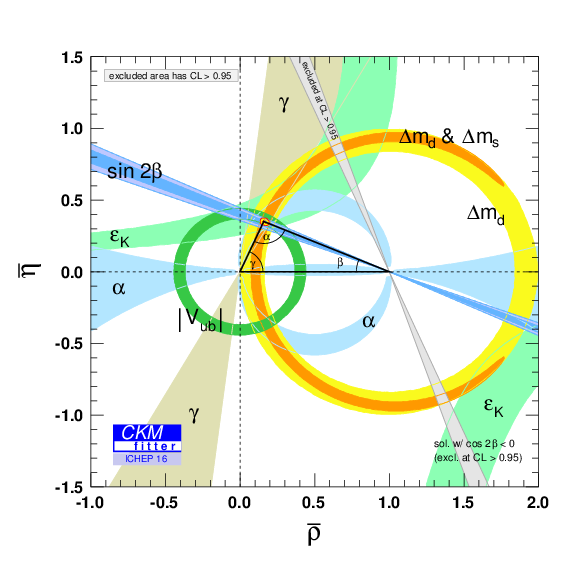
\includegraphics[scale=0.5]{figs/uut_CKMFitter.png}
\caption{Experimental constraints on the UUT, using the Wolfenstein parametrization ~\cite{CKMFitter}\label{fig:uutEXP}}
\end{center}
\end{figure}


\begin{comment}
The SUSY prolem and the MFV principle (Paradisi, Straub): The Bmu term will be complex at the high scale; thi is the approach that is commonly assumed e.g. in the CMSSM
\red{conclusion: not equivalent?}


\end{comment}
~\cite{Fellini4}



\chapter{LHCb}
\label{chap:LHCb}

\section{LHC}
\label{sec:LHC}
The Large Hadron Collider (LHC) is the world's largest and most powerful particle accelerator. Located at CERN (\textit{European Organization for Nuclear Research}), it consists of a 27 km ring of superconducting magnets with a number of accelerating structures, that boost the energy of the particles along the way. 

Two proton beams travelling in opposite directions collide at different points of the ring. These are extracted from ion sources, and accelerated in a chain of preaccelerators, being the lat stage of such chain the Super Proton Synchrotron (SPS) (see \figref{fig:LHC}). 
They are accelearted to produce collisions at energy in the center of mass ($\sqrt{s}$) of the order of the TeV, in order to test the Standard Model and look for New Physics. One of its main achievements has been the discovery of the Higgs boson, introduced in \red{refs}, the last piece of the Standard Model puzzle. Protons are sent on bunches containing up to $1.5\times 10^{11}$ particles, and corssing with a rate of 40 MHz. \red{check} Special runs with heavy ions (e.g. lead) are also made periodically. 
\begin{figure} [htb!]
\begin{center}
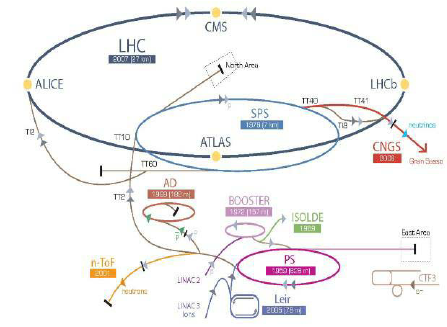
\includegraphics[scale=0.5]{figs/lhc.png}
\caption{The LHC injection complex. \label{fig:LHC}}
\end{center}
\end{figure}

%% Runs 
Since it first started operating in 2008, it has recorded data with different center of mass energies, corresponding to 2 data-taking periods: Run 1 (2009-2013,  $\sqrt{s}$ = 7, 8 TeV), and Run 2 (2013-present, $\sqrt{s}$ = 13, 14 TeV). An upgrade of the detectors was made in between the runs. \red{check}
%% Experiments

There are four interaction points within the LHC ring, corresponding to the four main experiments. In these points, the beams cross over to the other beam pipe and collide under a small angle. These four experiments are: \red{refs}

\begin{itemize}
\item \textbf{ATLAS} (\textit{A Toroidal LHC ApparatuS}): a general-purpose 4$\pi$ detector, focused mainly in the search of New Physics via direct searches and responsible of the Higgs boson discovery.
\item \textbf{CMS} (\textit{Compact Muon Solenoid}): also a general-purpose detector, with a physics program similar to ATLAS and a more compact layout. 
\item \textbf{ALICE} (\textit{A Large Ion Collider Experiment}): the smallest of the four detector, it focuses in heavy-ion studies. 
\item \textbf{LHCb} (\textit{Large Hadron Collider beauty}): a single-arm forward spectrometer, initially designed for the study of particles containing \bquark or \cquark quarks, now converted into a general-purpose detector. It is described in more detail in the following section. 
\end{itemize}


\section{LHCb}
\label{sec:LHCb}


The \lhcb detector~\cite{Alves:2008zz,LHCb-DP-2014-002} is a single-arm forward
spectrometer covering the \mbox{pseudorapidity} range $2<\eta <5$,
designed for the study of particles containing \bquark or \cquark
quarks. The detector includes a high-precision tracking system
consisting of a silicon-strip vertex detector surrounding the $pp$
interaction region~\cite{LHCb-DP-2014-001}\verb!*!, a large-area silicon-strip detector located
upstream of a dipole magnet with a bending power of about
$4{\mathrm{\,Tm}}$, and three stations of silicon-strip detectors and straw
drift tubes~\cite{LHCb-DP-2013-003}\verb!*! placed downstream of the magnet.
The tracking system provides a measurement of the momentum, \ptot, of charged particles with
a relative uncertainty that varies from 0.5\% at low momentum to 1.0\% at 200\gevc.
The minimum distance of a track to a primary vertex (PV), the impact parameter (IP),
is measured with a resolution of $(15+29/\pt)\mum$,
where \pt is the component of the momentum transverse to the beam, in\,\gevc.
Different types of charged hadrons are distinguished using information
from two ring-imaging Cherenkov detectors~\cite{LHCb-DP-2012-003}\verb!*!.
Photons, electrons and hadrons are identified by a calorimeter system consisting of
scintillating-pad and preshower detectors, an electromagnetic
calorimeter and a hadronic calorimeter. Muons are identified by a
system composed of alternating layers of iron and multiwire
proportional chambers~\cite{LHCb-DP-2012-002}\verb!*!.
The online event selection is performed by a trigger~\cite{LHCb-DP-2012-004}\verb!*!,
which consists of a hardware stage, based on information from the calorimeter and muon
systems, followed by a software stage, which applies a full event
reconstruction.

%%% LHC 
%%% LHCb : 
%% more details 
%% subdetector

\begin{figure} [htb!]
\begin{center}
%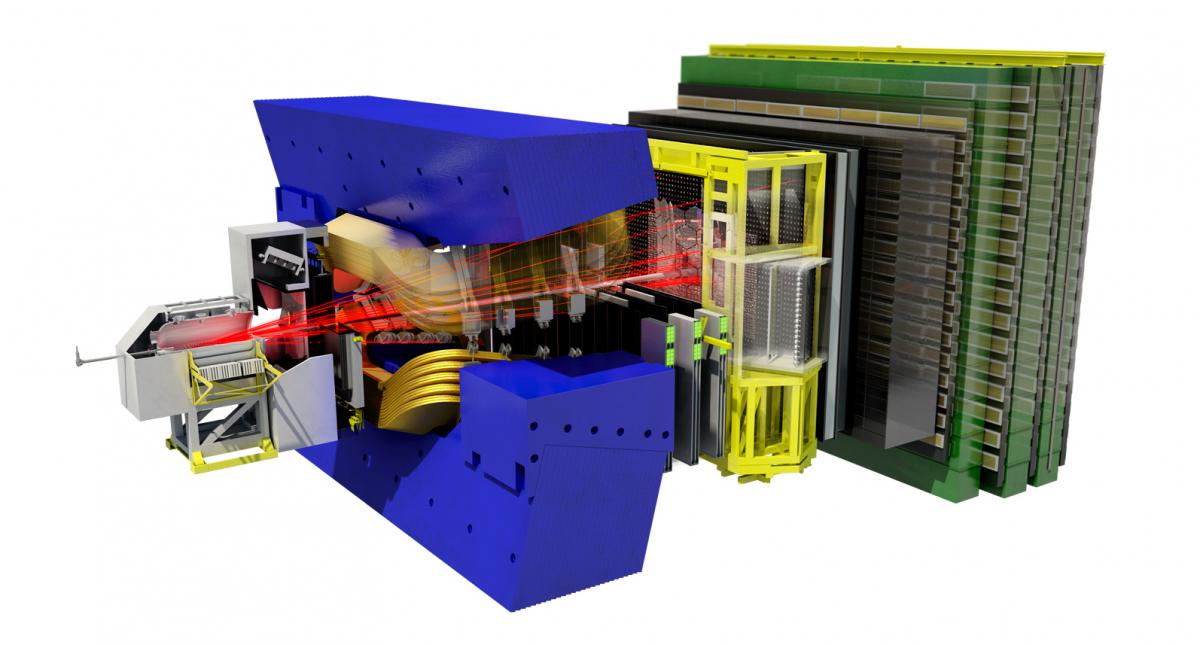
\includegraphics[scale=0.2]{figs/lhcb.jpg}
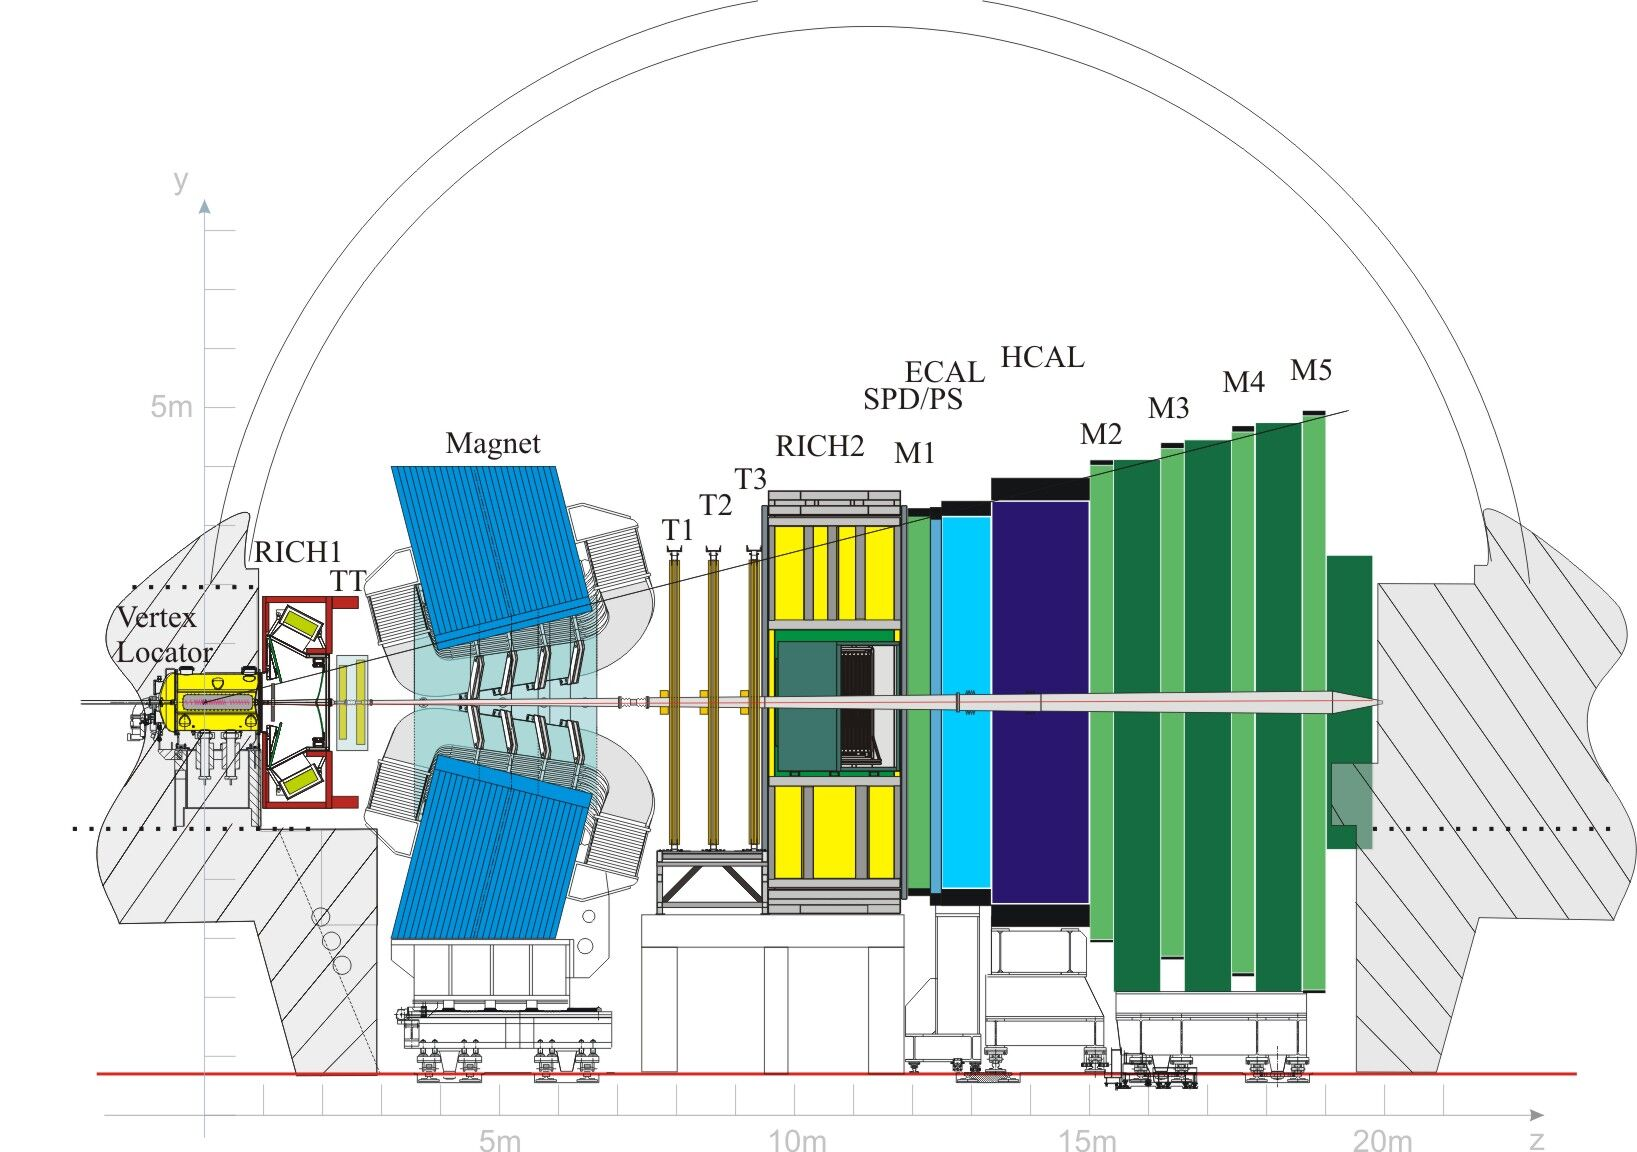
\includegraphics[scale=0.2]{figs/lhcb-slide.jpg}
\caption{LHCb detector \label{fig:LHCb}}
\end{center}
\end{figure}

\subsection{Beam pipe, vacuum chamber and BCM} % martes
The design of the beampipe (\ref{fig:beampipe}) is especially delicate, given the \red{pseudorapidity} region at which LHCb operates, where there is a high particle density. It is of 19m long and includes the forward window of the VELO and four main conical sectors. The three closer to the interaction point are made of beryllium, as it is highly transparent to particles resulting from collisions. The one left is made of stainless steel because of its good mechanical and vacuum properties. The beampipe support system consists of one fixed and one movable support, in order to reduce the background as much as possible. Two sector valves located at the cavern entrances isolate the experiment beam vaccum from the LHC.

The Beam Conditions Monitor (BCM) takes care of possible problems with the LHC beam conditions, requesting a beam dump if necessary. It monitors the particle flux at two locations close to the vacuum chamber (so as to protect the sensitive LHCb tracking devices). It is connected to the LHCb experiment control system and to the beam interlock controller of the LHC. The two stations consist of eight diamond sensors, with the same dimensions as those of ATLAS and CMS.
 
\begin{figure} [htb!]
\begin{center}
%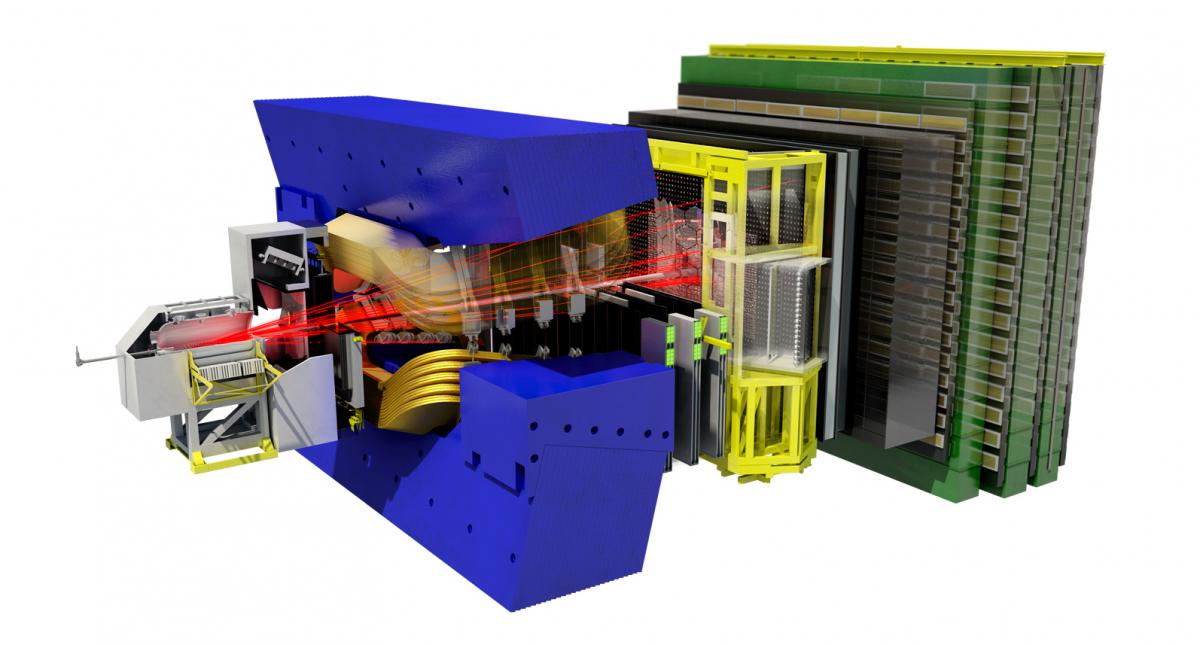
\includegraphics[scale=0.2]{figs/lhcb.jpg}
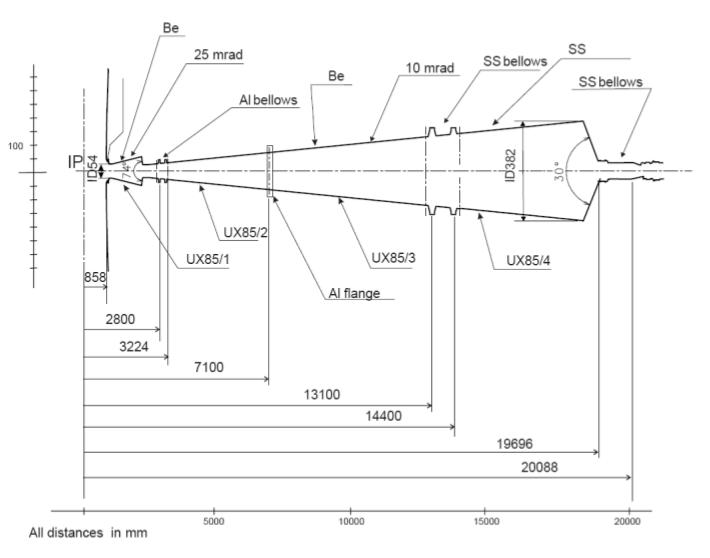
\includegraphics[scale=0.6]{figs/beampipe.png}
\caption{LHCb beam pipe \label{fig:beampipe}}
\end{center}
\end{figure}


\subsection{Magnet} % martes
LHCb contains a dipole magnet that bends charged particles in order to measure their momenta. The measurement covers the forward acceptance of $\pm 250 \rm mrad$ verticaly and of $\pm 300 \rm mrad$ horizontally. Two identical conical saddle-shaped coils surround an iron yoke, producing a magnetic field of 4 Tm for tracks of 10 m length (notice that difference parts of the detector need for different values of the magnetic field). These coils are made of pure Al-99.7. 

The magnet is operated using a Magnet Control System, a well as a Magnet Safety System, that takes care of the security of the magnet performance. 

The precision with which the magnetic field of the magnet is measured needs to be of the order of $10^{-4}$ so as to properly measure the momentum resolution of the charged particles. In order to ensure this, field mapping campaigns in the tracking volume were made and obtained a value of about $4\times 10^{-4}$ (\ref{fig:lhcbmagnet}). In order to reduce the systematic effects of the detector, \red{especially} for $CP$ studies, the polarity of the magnetic field needs to be changed periodically. 

\begin{figure} [htb!]
\begin{center}
%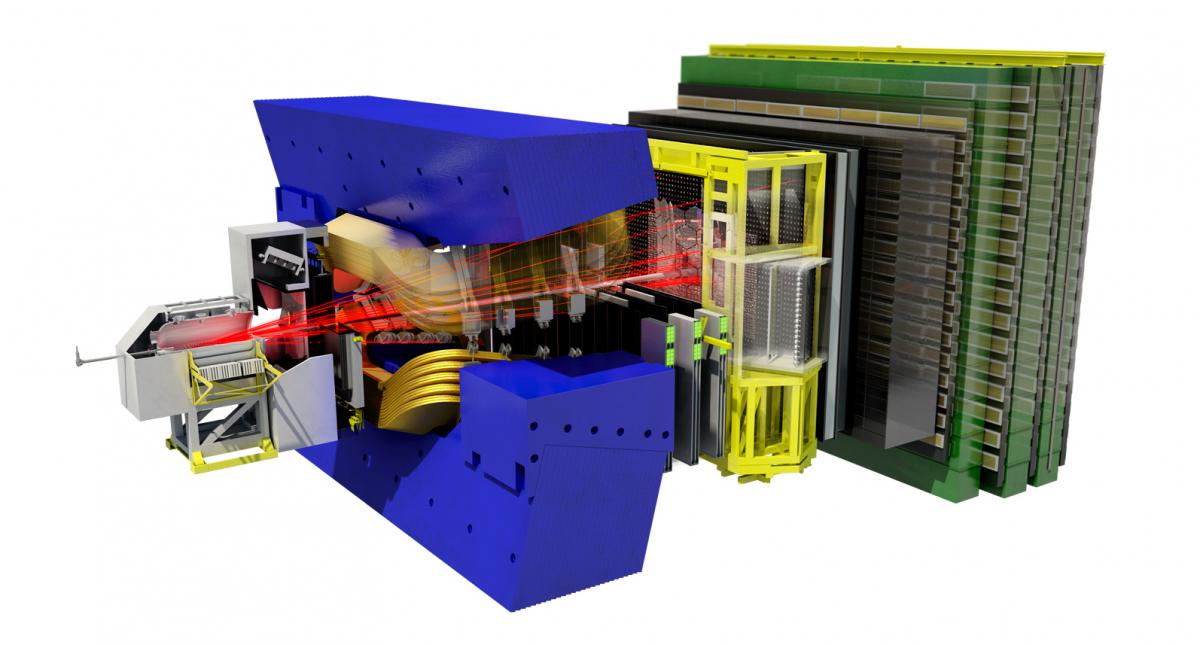
\includegraphics[scale=0.2]{figs/lhcb.jpg}
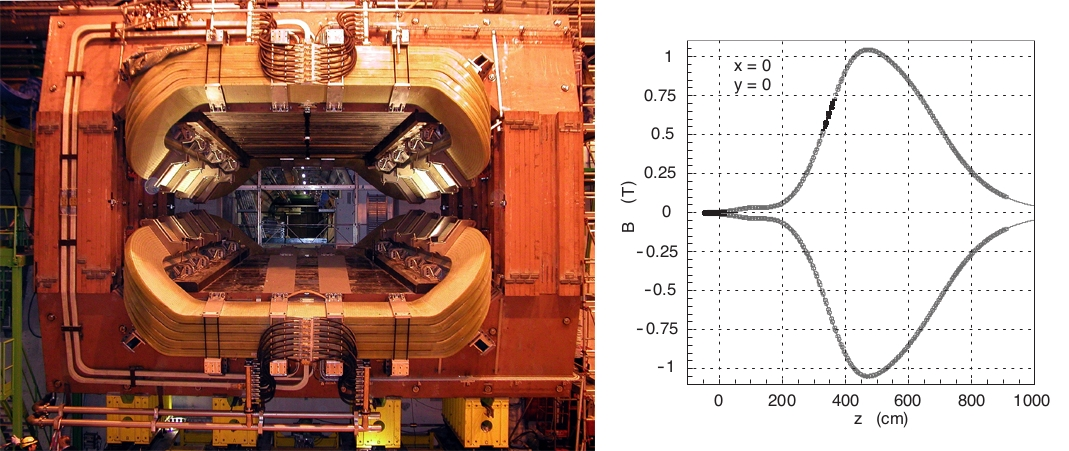
\includegraphics[scale=0.35]{figs/magnet.jpg}
\caption{LHCb magnet (left) and magnetic field along the z axis (right)\label{fig:lhcbmagnet}}
\end{center}
\end{figure}

\subsection{Tracking} %% martes, miercoles, jueves 
\label{sec:Tracking}
The tracking system of LHCb consists of two parts: the vertex locator (VELO) and four tracking stations: the \textit{Tracker Turicensis} (TT) upstream of the magnet, and T1-T3 downstream of the magnet. The latter are composed by an Inner Tracker (IT) and an Outer Tracker (OT). Both IT and TT belong to a common project, the \textit{Silicon Tracker} (ST). 

\subsubsection{VELO} 
The ability to reconstruct vertices with a high precision is a key feature of the LHCb detector. It is \red{vastly} used to accurately measure the decay lifetimes, the impact parameter and the flavour of the particles that are produced. Besides, detached vertices are of crucial importance for the High Level Trigger (\ref{sec:Trigger}). 

Such reconstruction is done in the VErtex LOcator (VELO), that provides measurements of the track coordinates close to the interaction region. It consists of 20 semicirular silicon modules located along the beam direction, each one providing measurement of cylindrical coordinates $(r,\phi)$ using microstrips, together with two planes perpendicular to the beam line, the \textit{pile-up veto system}, as it can be seen in \ref{fig:velo}, that are then used to get rid of high multiplicity events. The minimum pitch at the innermost radius
is $38  \rm \mu m$, increasing linearly to $101.6  \rm \mu m$ at the oter radius of 41.9mm . 
These sensors must be retractable, as the distance from them to the beam is smaller than the one required from LHC during the injection phase.  Vacuum inside the VELO is separated from the machine vacuum by corrugated aluminum foils, \textit{RF-foils}. 

The VELO was designed in order to fulfill the signal to noise ratio, efficiency, resolution and geometrical requirements. Polar coordinates are used in order to ensure fast reconstruction of tracks and vertices in the LHCb trigger~\cite{Alves:2008zz}.

\begin{figure} [htb!]
\begin{center}
%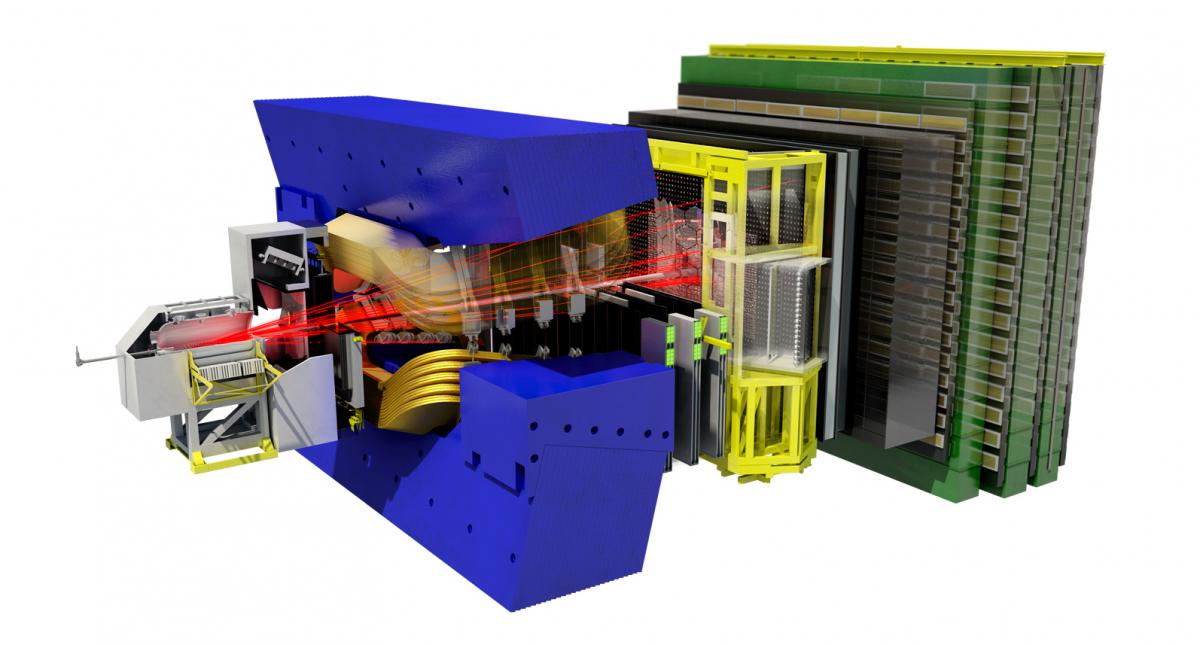
\includegraphics[scale=0.2]{figs/lhcb.jpg}
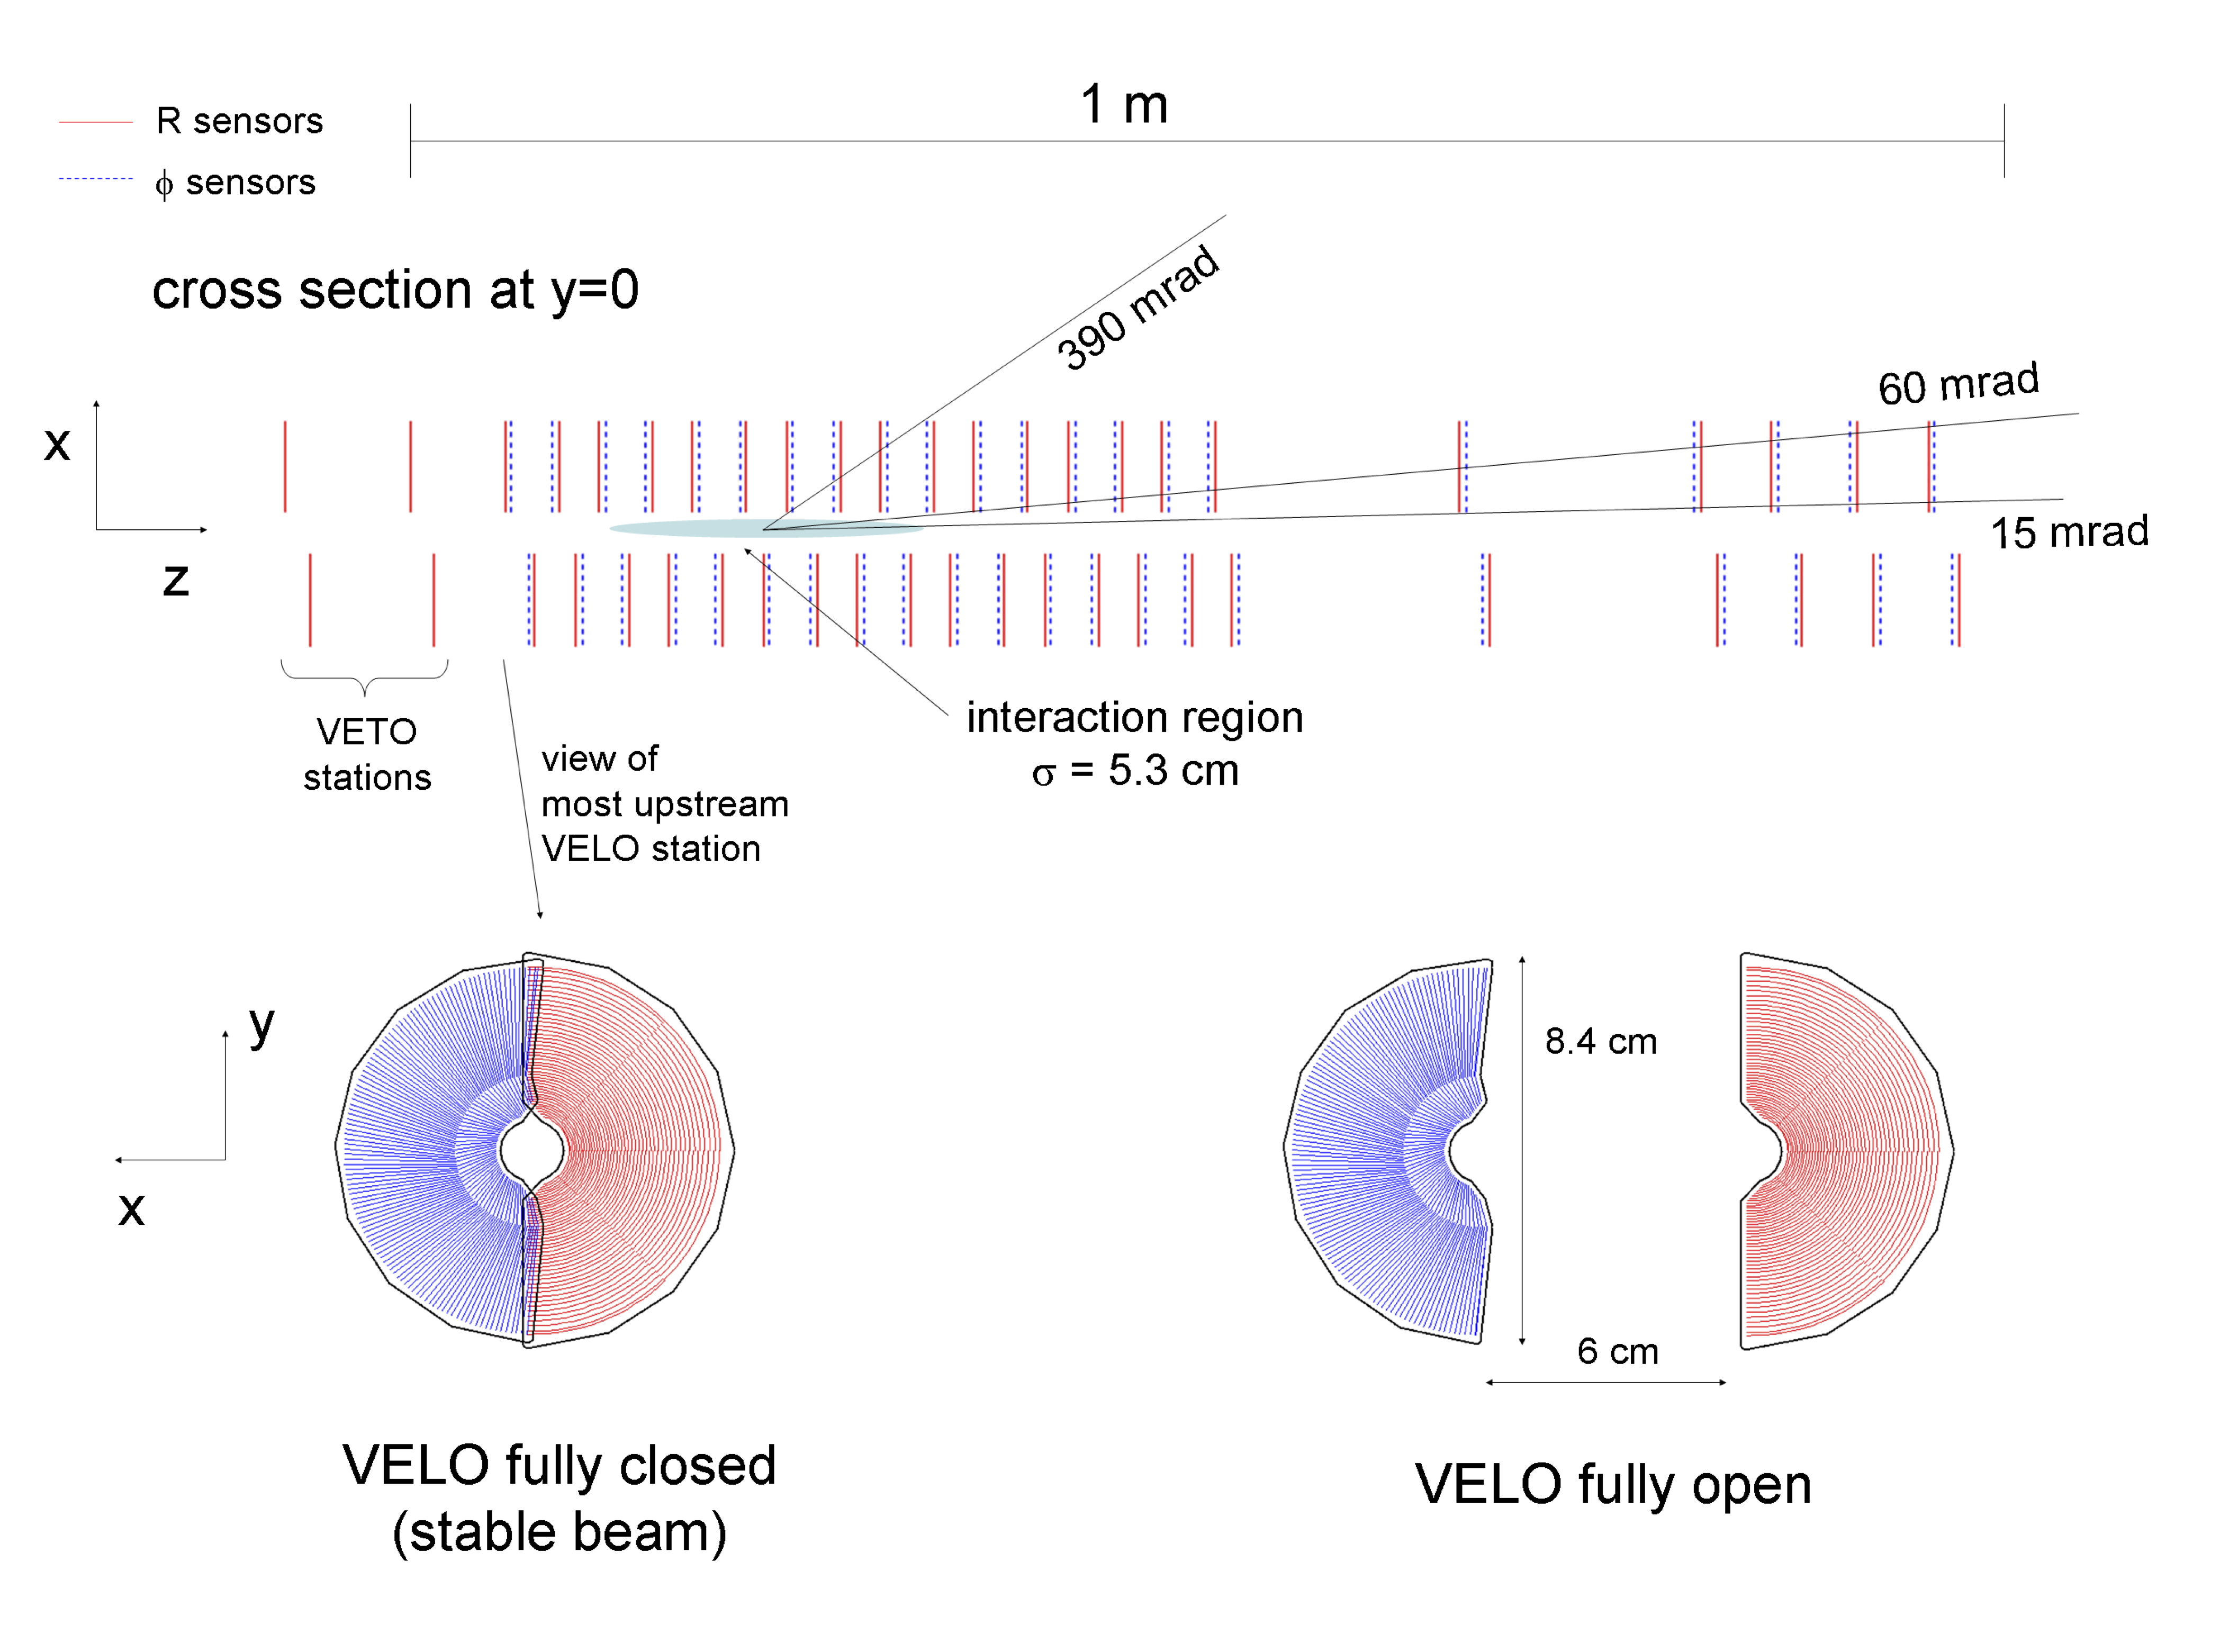
\includegraphics[scale=0.18]{figs/velo.png}
\caption{Cross section in the ($x$,$z$) plane of the VELO silicon sensors, at $y=0$, with the detector in the fully closed position. The front face of the first modules is also illustrated in both the closed and open positions~\cite{Alves:2008zz}.\label{fig:velo}}
\end{center}
\end{figure}

\subsubsection{ST} 
As said before, the Silicon Tracker (ST) refers to two different detectors: the Tracker Turicensis (formerly known as \textit{Trigger Tracker} (TT) and the Inner Tracker (IT) (see \ref{fig:lhcb_st}). Both use silicon microstrip sensors with a strip pitch of about 200 $\mu$m. 
The TT is a 150x130 cm high planar tracking station (covering the full LHCb acceptance), located upstream of the LHCb dipole magnet. The IT covers a 120x40 cm high cross shaped region in the centre of the three tracking stations downstream of the magnet. 

The TT and each of the three IT stations have four detection, organized in an (\textit{x-u-v-x}) configuration, with vertical strips in the first and the last layer. Strips in the second and third layer are rotated by a stereo angle of $-5^{\circ}$ and $5^{\circ}$ respectively (so as to get 3D reconstruction). The pitch is about $200\mu m$ which gives a single hit resolution of 50$\mu m$. Momentum resolution is then dominated by multiple scattering. The active area is of about $8.4m^2$ for the TT and of $4.0m^2$ for the IT. A temperature below $5^{\circ}\rm C$ is maintained in both cases.  

\begin{figure} [htb!]
\begin{center}
%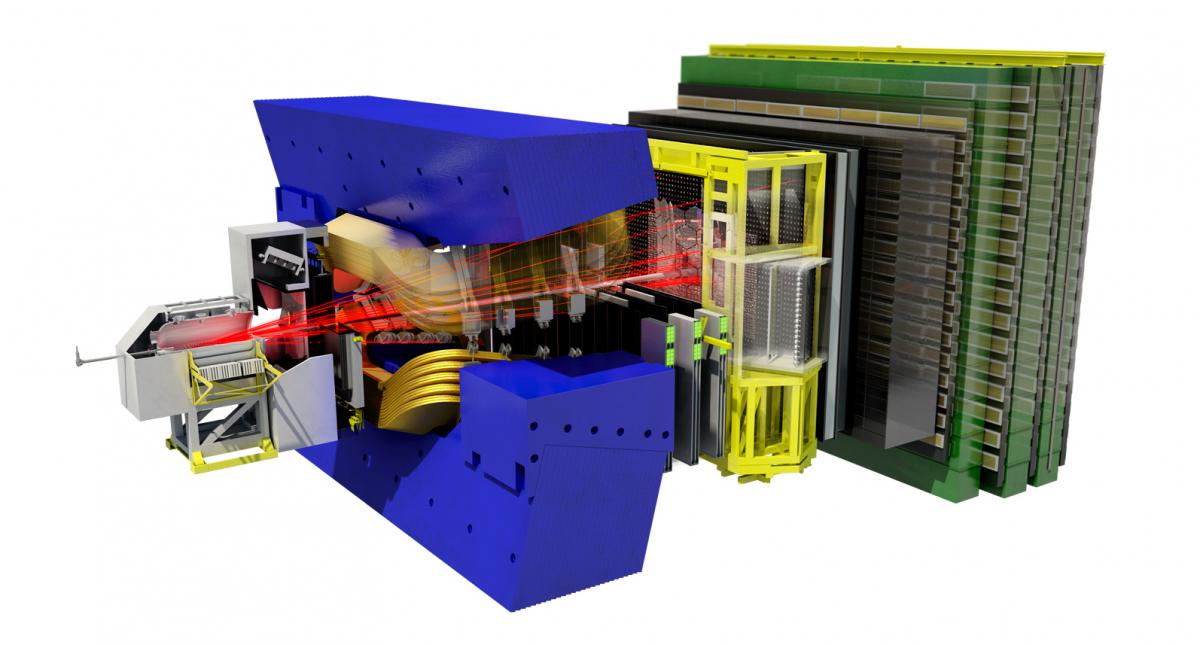
\includegraphics[scale=0.2]{figs/lhcb.jpg}
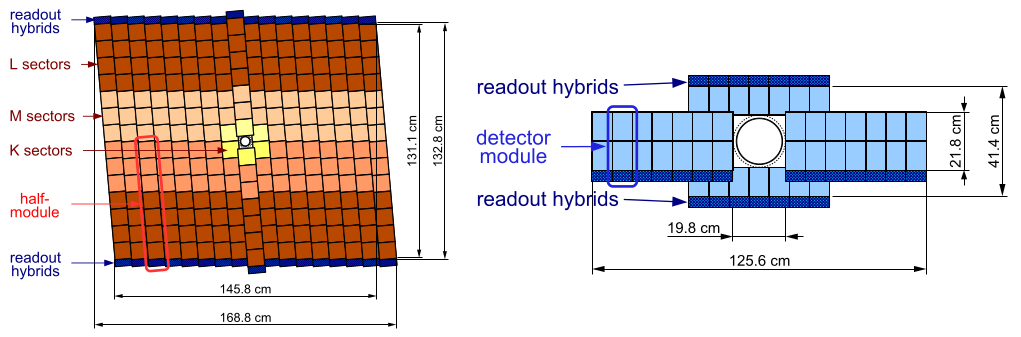
\includegraphics[scale=0.6]{figs/lhcb_st.png}
\caption{Layout of the third TT detection layer (left) and layout of an x detection layer in the second IT station (right)~\cite{Alves:2008zz}.\label{fig:lhcb_st}}
\end{center}
\end{figure}

\subsubsection{OT} % miercoles
The OT detector is designed for the tracking of charged particles, and the measurement of their momentum. Excellent momentum resolution and high tracking efficiency are needed for LHCb analyses. It consists \red{in} a drift-time detector, composed of an array of gas-tight straw-tube modules. For the gas, a mixture of Argon (70\%) and $CO_2$ (30\%) is used. This ensures a fast drift time, as well as a sufficient drift-coordinate resolution. 

The modules are arranged in three stations, each one consisting of four layers. The stations are further splitted in two halves, with two independently retractable units of two half layers (C-frames). Such arrrangement can be seen in \ref{fig:lhcb_ot}. 

\begin{figure} [htb!]
\begin{center}
%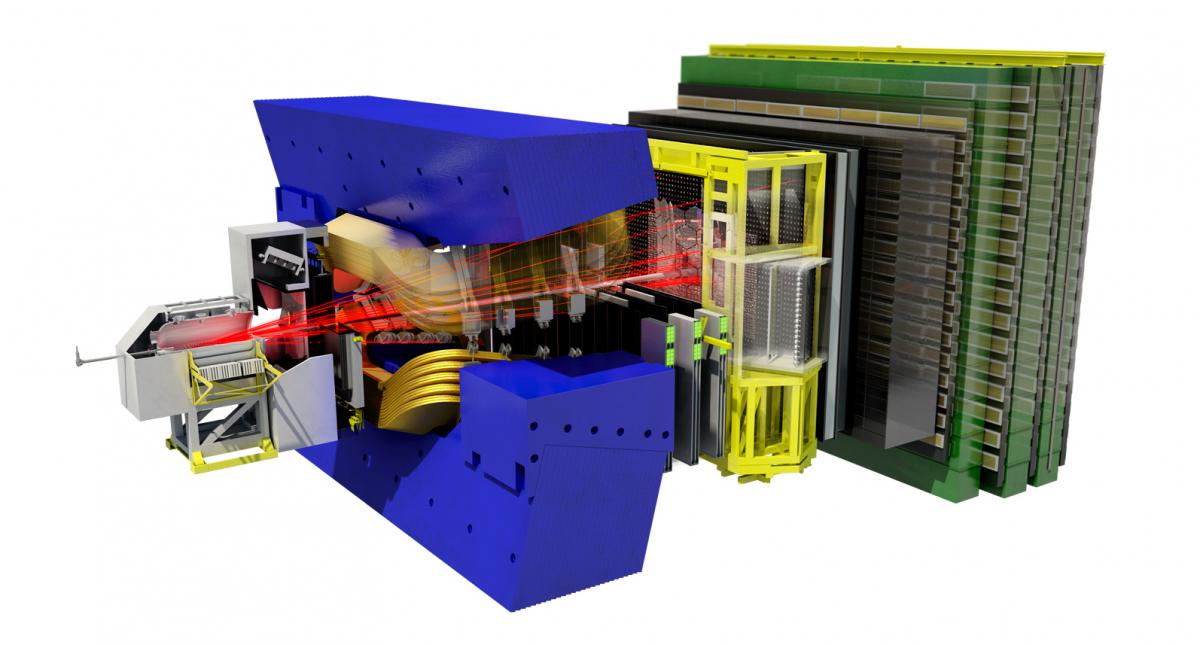
\includegraphics[scale=0.2]{figs/lhcb.jpg}
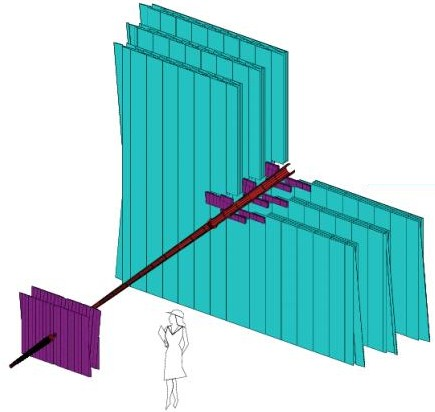
\includegraphics[scale=0.4]{figs/OT.jpg}
\caption{Arrangement of OT straw-tube modules in layer and stations~\cite{Alves:2008zz}.\label{fig:lhcb_ot}}
\end{center}
\end{figure}

\subsection{PID} % miercoles, jueves, viernes 
\label{sec:PID}
Particle identification (PID) at LHCb is crucial in order to properly distinguish the different types of particles that are detected. Particularly, it is important to further reduce backgrounds from different decays, as well as at the trigger level (\ref{sec:Trigger}). Three different subdetectors, described below, are used for PID.

\subsubsection{RICH}
There are two \textit{Ring Imaging Cherenkov detectors} at LHCb, designed to cover the full momentum range. RICH1 (\ref{fig:lhcb_rich} left) covers the low momentum charged particle range ($\sim 1-60 \rm GeV$), while RICH2 (\ref{fig:lhcb_rich} right) covers the high momentum charged particle range ($\sim 15\rm GeV$ up to and beyond $\sim 100\rm GeV$). In order to do this, RICH1 (located upstream, between the VELO and the Trigger Tracker) uses aerogel and $\rm C_4F_{10}$ radiators, while the downstream detector, RICH2, uses a $\rm CF_4$ radiator. 

While RICH1 covers the ful LHCb acceptance, from $\pm 25 \rm rad$ to $\pm 300 \rm rad$ horizontal and $\pm 250 \rm rad$ vertical, RICH2 has a more limited angular acceptance (where the high momentum particles are produced), of $\sim \pm 15 \rm rad$ to $\pm 120 \rm rad$ horizontal and $\pm 100 \rm rad$.

\begin{figure} [htb!]
\begin{center}
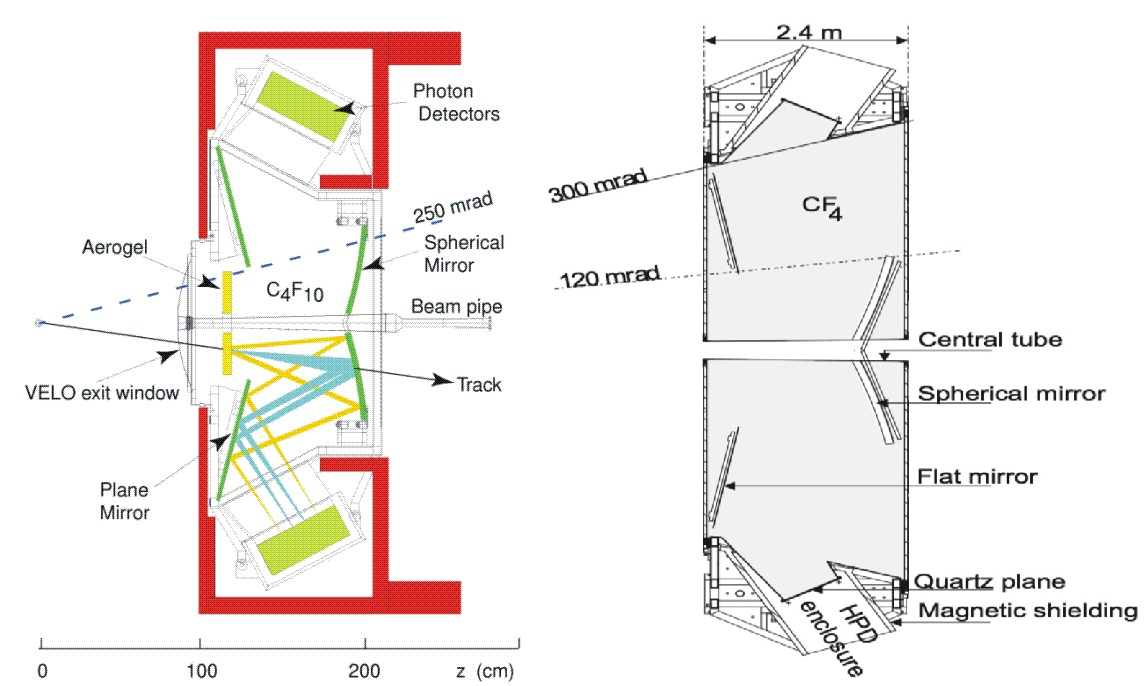
\includegraphics[scale=1.5]{figs/RICH.png}
\caption{Schematic view of  RICH1 (left) and RICH2 (right) detectors~\cite{Alves:2008zz}.\label{fig:lhcb_rich}}
\end{center}
\end{figure}

Both detector use spherical and flat mirrors to focus the Cherenkov light. The optical layout is vertical for RICH1 and horizontal for RICH2. Cherenkov photons in the wavelength range 200-600 nm are detected by Hybrid Photon Detectors (HPDs), which are outside the LHCb acceptnce. These are surrounded by external iron shields that shield tem from the \red{fringe,marginal?} field of the LHCb dipole. 
%%% The spherical mirrors are located within the LHCB acceptance and are traversed by charged particles and photons 

\subsubsection{Calorimeters} % miercoles
The transverse energy of hadrons, electrons and photons is measured and selected in the calorimeter for the L0 trigger (\ref{sec:Trigger}). The energy and position is also measured for these particles, which are identified in this subdetector, while avoiding the pass of those particles to the muon system. The proper identification of hadrons, electrons and photons is also of great importance for correctly identifying the flavour of the original meson in the decay (\textit{flavour tagging}). This is done taking into account that these particles deposit the energy in the different parts of the calorimeter in a different manner. 
 
It consists of two separate parts: an electromagnetic calorimeter (ECAL) followed by a hadron calorimeter (HCAL), to identify electromagnetic and hadronic showers, respectively. A preshower detector (PS) is located before the ECAL, in order to eliminate a large background of charged pions that could be misidentified as elecrons. In front of the PS, a scintillator pad detector (SPD), used to select charged particles, is located. For all these parts a variable lateral segmentation is adopted, given that the hit density varies by two orders of magnitude over the calorimeter surface ~\cite{Alves:2008zz}. Because of the dimensions of the hadronic showers, the HCAL is segmented into two zones with larger cell sizes. 

In all cases, the same principle of scintillation light transmitted to a Photo-Multiplier (PMT) (that turn this light into an electric ignal) by wavelength-shifting (WLS) fibres is adopted. To have a constant transverse energy cale the gain in the ECAL and HCAL phototubes is set in proportion to their distance to the beampipe.  

\begin{figure} [htb!]
\begin{center}
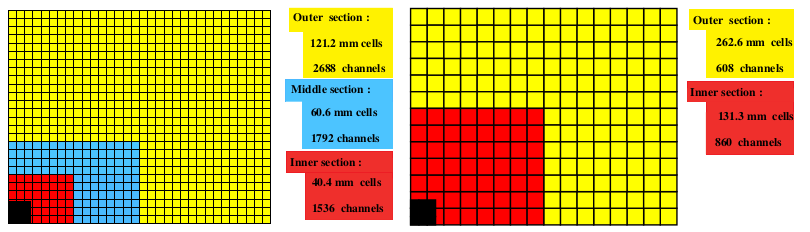
\includegraphics[scale=0.7]{figs/CALO.png}
\caption{Lateral segmentation of the SPD/PS and ECAL (left) and the HCAL (right). One quarter of the detector front face is shown~\cite{Alves:2008zz}.\label{fig:lhcb_calo}}
\end{center}
\end{figure}
\red{dimensions?}

\subsubsection{Muon System} 
The muon system provides fast information for the high-$p_T$ muon trigger at the earliest level (L0) and muon identification for the high-level trigger (HLT) and offline analysis~\cite{Alves:2008zz}. Given that muons are present in final states of the most relevant channels for LHCb, this is of crucial importance.

It is composed of five rectangular stations (M1-M5), located along the beam axis, with a total of 1380 chambers and 435$\rm m^2$ of coverage. The inner and outer angular acceeptances are 20(16) mrad and 306(258) mrad in the bending (non-bending) plane respectively~\cite{Alves:2008zz}. All the stations are divided into 4 regions, R1-R4, with increasing distance from the beam axis. Their dimensions (scaling a factor two  from one region to the next) and their geometry provide the same flux and channel ocupancy for all of them. Muti-wire proportional chambers (MWPC) are used for all regions except the inner region of station M1, where triple-GEM detectors (consisting of three gas electron multipliers) are used. 

Stations M2 to M5 are placed downstream the calorimeters, interleaved with three iron filters. They have a threshold of $\sim 6 \rm GeV/c$ for a muon to cross the five stations. Stations M1-M3 are used to define the track direction and to calculate the $p_T$ of the candidate muon, due to their high spatial resolution along the bending plane. \red{On the other hand}, stations M4 and M5 are focused on identifying penetrating particles. Station M1 is located in front of the calorimeters. Its function is to improve the $p_T$ measurement in the trigger. The geometry of all the stations is such that all their transverse dimensions scale with the distance from the interaction point. %% A fourth station is situated after M5 to remove machine related background 


%%% The muon stations are equipped with Multi Wire Proportional Chambers [98] (MWPCs) operating
%% with an Ar:CO 2 :CF 4 (40%:55%:5 % in volume) gas mixture. The only exception to the MWPCs is the
%% innermost region R1 of the station M1, in which the high rate of particles requires the use of a triple-
%% GEM detector, which consists of three gas electron multiplier (GEM), using Ar:CO 2 :CF 4 (45%:15%:40%
%%% in volume) as a gas mixture.

\begin{figure} [htb!]
\begin{center}
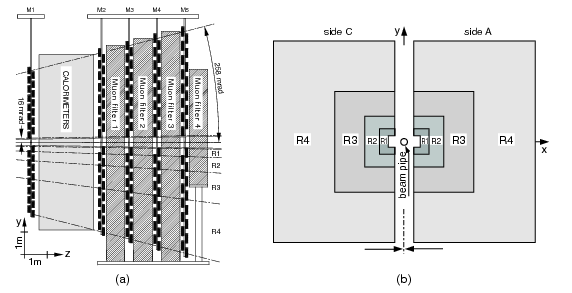
\includegraphics[scale=1.0]{figs/MUON.png}
\caption{(a) Side view of the LHCb Muon Detector. (b) Station layout with the four regions R1-R4~\cite{Alves:2012ey}.\label{fig:lhcb_muon}}
\end{center}
\end{figure}

\subsection{Trigger} 
\label{sec:Trigger}
The LHCb trigger is one of the most important part of its infrastructure, as it allows for a reduction of the crossing frequency with interactions visible by the spectrometer from 10MHz to about 2 - 5 kHz, at which rate the events are written to storage for further offline analysis~\cite{Alves:2008zz}. It is composed by two levels: Level-0 (L0) and the High Level Trigger (HLT). Both parts are optimised to obtain the highest efficiency for the events selected in the offline analysis, while avoiding storage of as much background events as possible. 

\subsubsection{L0}
The purpose of this first stage of the trigger is to reduce the LHC beam crossing rate of 40 MHz to 1MHz, with which the entire detector can be read out ~\cite{Alves:2008zz}. This is done reconstructing the highest $E_T$ hadron, electron and photon clusters in the calorimeters, together with the the two highest $p_T$ muons in the muon chambers, as B meson decay products are expected to have large $p_T$ and $E_T$. A pile-up system in the VELO estimates the number of primary pp interactions in each bunch crossing. The calorimeters calculate the total observed energy and an estimate for the number of tracks, based on the number of hits in the SPD. With this, unwanted events are discarded. 

It is composed by three parts, all connected to a different part of the LHCb, and all connected to the L0 DU (see \ref{fig:lhcb_L0}):

\begin{enumerate}
\item The pile-up system: its purpose is dinstinguishing crossings with single and multiple visible interactions. For this, it uses four silicon sensors as the ones used in the VELO, that measure the radial position of the tracks.  It consists of two silicon planes, situated upstream of the VELO and perpendicular to the beam-line, where the radii of track hits are measured.  From this, the position of the track origin on the beam axis (the \textit{vertex}) can be reconstructed.  %%%% two overlapping velo R-sensors which have strips at constant radii, and each strip covers 45 degrees
\item The L0 calorimeter trigger: its goal is to look for high $E_T$ electrons, photons, neutral pions or hadrons. This is done forming clusters by adding the transverse energy of 2x2 cells and selecting the cluster with the highest $E_T$. This zone is large enough to contin most of the energy, while avoiding overlapping \red{among} different particles. Afterwards, such cluster is identified as one of the particle types using information from the SPD, PS, ECAL and HCAL subdetectors. 
\item The L0 muon trigger: in the muon chambers muons are reconstructed with a resolution in $p_T$ of $\sim 20\%$. The L0 muon trigger selects the two muons with the highest $p_T$ for each quadrant of the muon detector. The track finding is performed on the logical pads, searching for hits defining a straight line through the fivve muon stations and pointing towards the interaction point~\cite{Alves:2008zz}, also enabling the determination of the $p_T$ of the track.  %%% Seeds of the track finding algorithm are hits in M3. For each logical pd hit in M3, an extrapolated position is set in M2, M3 and M5, long a straight line passing thorugh the hit and the interaction point. 
\end{enumerate}
Multiplicities are measured by the SPD cells.
\red{charged track multiplicity}

A L0 Decision Unit (DU) collects all the information and derives the final L0 trigger decision for each bunch crossing to the Readout Supervisor , allowing for overlapping of several trigger conditions, as well as for prescaling. The Readout Supervisor is in chrage of the ultimate decision about whether to accept an event or not. 

The L0 uses custom made electronics, fully synchronous with the 40 MHz bunch crossing signal of the LHC. All L0 electronics uses fully custom-designed boards that use parallelism and \red{pipelining} in order to speed up the process. The time passed between a pp interaction and the arrival of the L0 trigger decision is of 4 $\mu$s, that leaves 2$\mu$s for data processing in the L0.

\begin{figure} [htb!]
\begin{center}
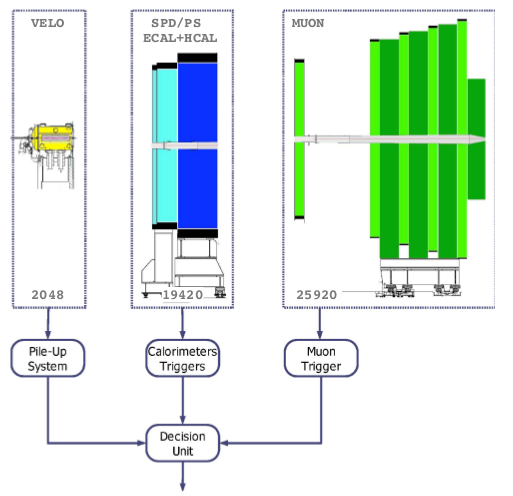
\includegraphics[scale=0.7]{figs/L0.png}
\caption{Overview of the L0~\cite{Alves:2008zz}.\label{fig:lhcb_L0}}
\end{center}
\end{figure}



\subsubsection{HLT} 
%% processor farm
The High Level Trigger (HLT) reduces the event rate from 1MHz down to 2 - 5 kHz, making use of the full event data. The HLT selected events are then saved on permanent storage. The algorithms that it uses refine candidates found by the L0 and divide them into independent \textit{alleys}, selected from the L0 decision, requiring the candidate tracks to be reconstructed in the VELO and/or the T-tations. With this, the rate is reduced to about 30kHz, where it becomes interesting to take into account both inclusive and exclusive criteria. It is further subdivided into HLT1 and HLT2, each with different purposes. The overall flow of all the trigger steps can be seen in \ref{fig:lhcb_HLT}. 

It consists of a C++ application that runs on over \red{2000} computing nodes, the Event Filter Farm (EFF). Even though it can access all data in one event, the purpose is to discard uninteresting event using part of the full event data. The cuts applied at this stage are generally very loose compared to the offline analysis, so as to be able to study the sensitivity of the selections and to profit from refinements due to improved calibration constants. \red{In order to compute systematic uncertainties and trigger efficiencies, both levels can be fully emulated on stored data. }

\begin{figure} [htb!]
\begin{center}
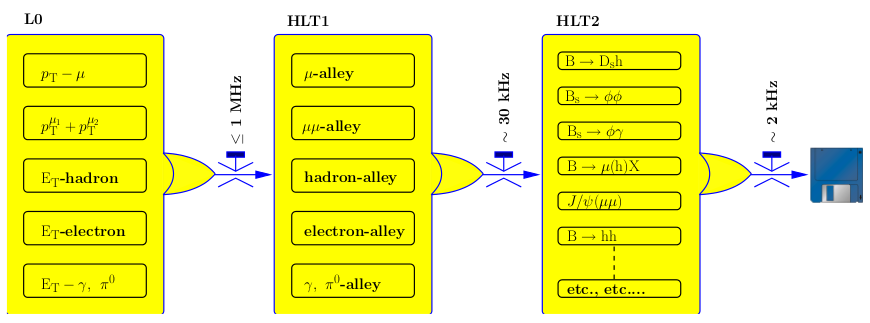
\includegraphics[scale=0.7]{figs/HLT.png}
\caption{Flow-diagram of the different trigger sequences~\cite{Alves:2008zz}.\label{fig:lhcb_HLT}}
\end{center}
\end{figure}

Both HLT1 and HLT2 summaries, containing the information of all tracks and vertexes that triggered events, are stored. This allows the study of the trigger performance, as well as of the trigger source of each event. Furthermore, in order to ensure the traceability of the trigger condiions in the off-line analysis, the combination of trigger algorithms with their selection parameters are pre-loaded in the EFF before a fill in a Trigger Configuration Key (TCK). 

\subsubsection{HLT1} 
\label{sec:HLT1}
The main goal of HLT1 is the so-called L0 confirmation, to reconstruct particle in the VELO and T-stations correspondence to the L0 objects, or for neutral particles to confirm de absence of a charged particle that could be associated to these same objects. Different reconstruction sequences (\textit{alleys}) with different algorithms and selection cuts are applied according to the L0 candidate type. The events can pass by more than one alley, provided that they are selected by multiple triggers. 
\subsubsection{HLT2}
At this stage of the trigger, a set of tracks is selected with very broad cuts on their momentum and impact parameter, and used to form composite particles. \red{These are then used for all selections to avoid duplication in the creation of final states.} The selections can be exclusive or inclusive, depending on whether the full final state is reconstructed or not. The inclusive triggers are less dependent on the on-line reconstruction, while the exclusive one produces a smaller rate, thus allowing for a more relaxed set of cuts.  
\label{sec:HLT2}

%% online and simulation? 

%\subsection{Performance} % s2
\subsection{Tracking and Vertexing performance}
\label{sec:TrackingPerformance}
In the track reconstruction software the hits in the VELO, the TT, the IT and the OT detectors are combined to form particle trajectories from the VELO to the calorimeters, with the purpose of finding all tracks in the event wihich leave sufficient detector hits. Depending on the subdetectors used for the reconstruction, offline tracks are classified in the following categories (see \ref{fig:lhcb_Tracks}): 

\begin{itemize}
\item \textbf{Long tracks}: those that traverse the VELO, the TT and the T-stations, hence having the most precise momentum determination. 
\item \textbf{Upstream tracks}: those traversing only the VELO and TT stations. Generally, they have lower momentum and are bent out of the detector acceptance by the magnetic field. Nevertheless, they pass through the RICH1 detector. Hence, they may generate Cherenkov photons, nd cn be used to understand backgrounds. Besides, they can also be used for flavour tagging, albeit their momentum resolution is poor.
\item \textbf{Downstream tracks}: travering only the TT and T stations. The most relevant cases are the decay products of $K_S^0$ and $\Lambda$ that decay outside of the VELO acceptance. 
\item \textbf{VELO tracks}: measured in the VELO only and typically with large angle, or backward trakcs. They are useful for the primary vertex reconstruction. 
\item \textbf{T tracks}: the ones measured in the T stations, typically produced in secondary interactions, but useful for the global pattern recognition in RICH2. 
\end{itemize}
For $K_S^0$ reconstruction, only long tracks and downstream tracks are used. 

\begin{figure} [htb!]
\begin{center}
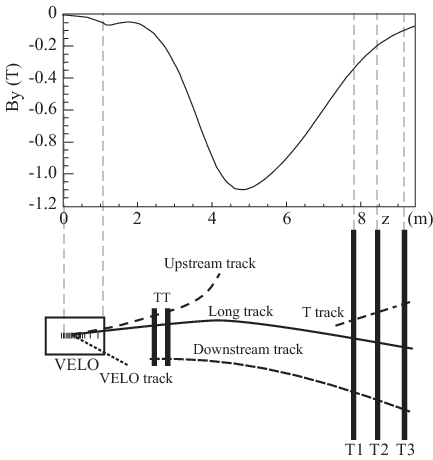
\includegraphics[scale=0.6]{figs/TrackTypes.png}
\caption{Schematic illustration of the various track types. For reference the main \textit{B}-field component ($B_y$) os plotted above as a function of the \textit{z} coordinate~\cite{Aaij:2014jba}.\label{fig:lhcb_Tracks}}
\end{center}
\end{figure}

For the track reconstruction algorithm, track \textit{seeds} are used as starting points. These are the initial track candidates in the VELO and T stations, where the magnetic field is low. Their trajectories are refitted using the Kalman filter \red{ref}, that accounts for multiple scattering and energy loss. The quality os such fitting is monitored using the $\chi^2$ of the fit and the \textit{pull} distribution for the different parameters. 

The pattern recognition performance is evaluated in terms of efficiencies and ghost rates. The efficiencies are the ratio of successfully reconstructed tracks over the total amount of reconstructible tracks. A track is considered recontructible if it has a minimum number of hits in the relevant subdetector, and \textit{successfully reconstructed} if at least 70\% of such hits originate from a single MonteCarlo (simulated) particle. Otherwise, it is considered a \textit{ghost track}. 

Figure \ref{fig:lhcb_TrackEfficiency} shows this efficiency as a function of two kinetic variables, namely the momentum, \textit{p}, and the pseudorapidity, \textit{eta}, for 2011 and 2012. The performance in the 2012 data is slightly worse, which is partially due to the higher hit multiplicity at the higher centre-of-mass energy~\cite{Aaij:2014jba}. The average efficiency is above 96\% for $5 \rm GeV/c < p < 200 \rm GeV/c$, $2 < \eta < 2$, thus covering the LHCb phase space. 

\begin{figure} [htb!]
\begin{center}
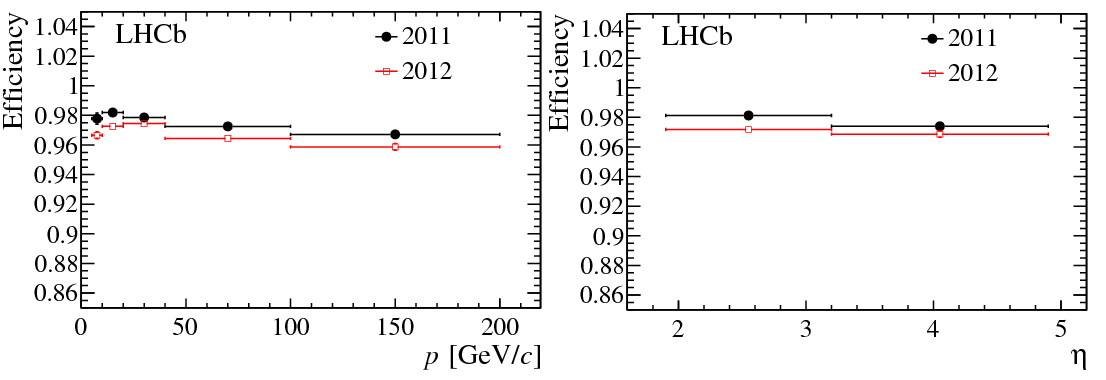
\includegraphics[scale=0.5]{figs/Efficiency_p_eta.png}
\caption{Tracking efficiency on muons from $J/\psi$ as a function of momentum (left) and
pseudorapidity (right). Black points correspond to 2011 data and red 2012 data
~\cite{Aaij:2014jba}.\label{fig:lhcb_TrackEfficiency}}
\end{center}
\end{figure}

As for the relative momentum resolution, as it is shown in \ref{fig:lhcb_Resolution} for two muons coming from a $J/\psi$,it is better (about 5 per mille) for low-momentum than for high-momentum (about 8 per mille) ranges. Hence, the best performances in terms of momentum resolution are achieved for long tracks, as said before. 

\begin{figure} [htb!]
\begin{center}
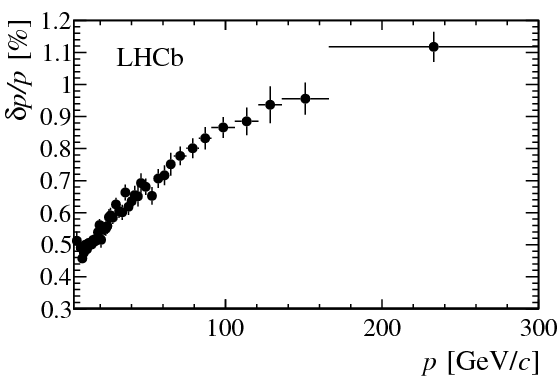
\includegraphics[scale=0.5]{figs/Resolution_p.png}
\caption{Relative momentum resolution versus momentum for long tracks in data obtained using $J/\psi$ decays~\cite{Aaij:2014jba}.\label{fig:lhcb_Resolution}}
\end{center}
\end{figure}

In order to assess the vertexing performance at LHCb, two main quantities are examined: the primary vertex (PV) resolution, and the impact parameter. The PV resolution is measured by comparing two independent measurements of the vertex position in the same event. This is achieved by randomly splitting the set of tracks in an event into two and reconstructing the PVs in both sets. 

The impact parameter (IP) of a track is defined as its distance from the primary vertex
at its point of closest approach to the primary vertex. Particles resulting from the decay
of long lived \textit{B} or \textit{D} mesons tend to have larger IP than those of particles produced at the primary vertex. Selections on IP and the IP $\chi^2$ are extensively used in LHCb analyses to reduce the contamination from prompt backgrounds. Consequently, an optimal IP resolution and a good understanding of the effects contributing to the IP resolution are of prime importance to LHCb performance~\cite{Aaij:2014jba}.

The IP resolution is governed by three main factors: multiple scattering of particles by
the detector material; the resolution on the position of hits in the detector from which
tracks are reconstructed; and the distance of extrapolation of a track between its first hit in the detector and the interaction point. The minimisation of these factors is achieved in the design of the VELO~\cite{Aaij:2014jba}. %The sensors are positioned close to the beams, separated from them by only a thin aluminium foil. The first active strips are only 8 mm away from the beams during physics collisions. 

The left part of figure \ref{fig:lhcb_PV_IP} shows the PV resolution in the \textit{x} and \textit{y} direction as a function of the number of tracks. It can be seen that in both cases it immproves with the number of tracks. The right part shows the IP resolution in the \textit{x} direction as a function of the inverse of the transverse momentum. Very good resolution is achieved in the VELO, thanks to \red{the silicon strips}. 

\begin{figure} [htb!]
\begin{center}
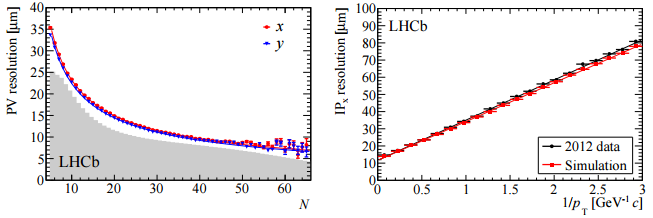
\includegraphics[scale=1.0]{figs/PV_IP.png}
\caption{The primary vertex resolution (left), for events with one reconstructed primary vertex, as a function of track multiplicity. The \textit{x} (red) and \textit{y} (blue) resolutions are separately shown and the superimposed histogram shows the distribution of number of tracks per reconstructed primary vertex for all events that pass the high level trigger. The impact parameter in \textit{x} resolution as a function of $1/p_T$ (right). Both plots are made using data collected in 2012.~\cite{Aaij:2014jba}.\label{fig:lhcb_PV_IP}}
\end{center}
\end{figure}

\subsection{PID performance} %% 2 dias s2
\label{sec:PIDPerformance}
As explained in \ref{subsec:PID}, particle identification at LHCb is performed in 4 different subdetectors. Each one of them gives a different performance that is then further combined into an overall PID performance. 

For the calorimeters the main role is to distinguish photons, electrons and neutral pions. Electrons are differentiated from photons and $\pi^0$ in the fact that they have a track associated before the energetic deposit in the calorimeter, as they are charged particles. Their associated likelihood is estimated using information from the ECAL, the PS and the HCAL. 
In order to separate photons from $\pi^0$, a neural network clasifier is used, trained with \red{pure samples}. Non-converted photons are identified using a photon hypothesis likelihood, employing variables from the different subdetectors (PS and ECAL). %%% DLL?

Both for photons and for electrons, the PID performance is assessed using the log-likelihood difference between the signal hypothesis (photon or electron) versus the background one (hadrons for electrons). In the cae of the electrons, this log-likelihood is computed as the sum of log likelihoods:
\begin{equation}
\Delta \log{\mathcal{L}^{\rm CALO}(e-h)} = \Delta \log{\mathcal{L}^{\rm ECAL}(e-h)} + \Delta \log{\mathcal{L}^{\rm HCAL}(e-h)} + \Delta \log{\mathcal{L}^{\rm PS}(e-h)} 
\end{equation}

This is shown in \ref{fig:PID2}, for different cuts. As expected, the higher momenta particles have higher misidentification rates. 
\begin{figure} [htb!]
\begin{center}
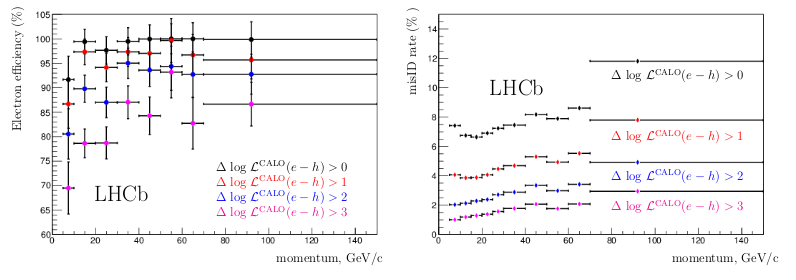
\includegraphics[scale=0.8]{figs/PID2.png}
\caption{Electron identification performances for various $\Delta\log{\mathcal{L}^{\rm CALO}(e-h)}$ cut: electron efficiency (left) and misidentification rate (right) as functions of the track momentum~\cite{Aaij:2014jba}.\label{fig:PID2}}
\end{center}
\end{figure}

%\red{FIGREF} shows the ratio of photon detection efficiencies between converted and non-converted photons coming from the decay of $\pi^0$ mesons for both simuation and data. As it can be seen, simulation properly reproduces the data distribution, and the reconstruction algorithms work equally well in data and simulation., PID1 

As for the RICH, its mission is to distinguish charged hadrons ($\pi$,$K$,$p$). The information thus obtained is used at the final analysis level and as part of the software level of the trigger. Complementary information on charged leptons can also be provided by the RICH. Its performance is evaluated using two variables:
\begin{itemize}
\item The Cherenkov angle resolution, $\theta{(\sigma_C)}$, defined as the resolution of the Cherenkov angle with which the emitted photons can be reconstructed. 
\item The photoelectron yield, defined as the average number of detected photons for each track traversing the Cherenkov radiator media. 
\end{itemize}

Because of te high average track multiplicity in LHCb events, a reconstructed Cherenkov ring will generally overlap with several neighbouring rings. Figure \ref{fig:PID3} shows the Cherenkov angle as a function of particle momentum using information from the raditor for isolated tracks selected in data. As expected, different bands represent different masses, hence different particles. 

\begin{figure} [htb!]
\begin{center}
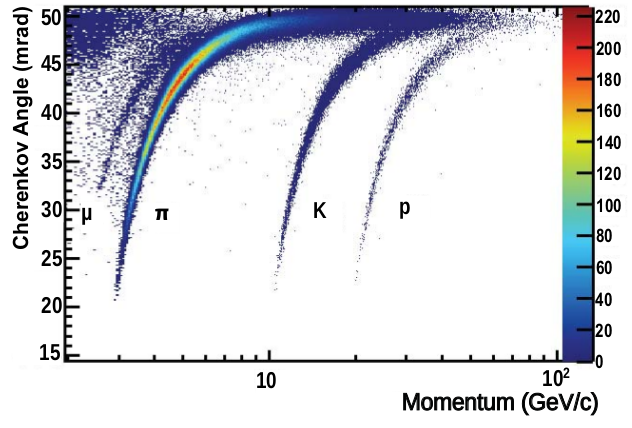
\includegraphics[scale=0.7]{figs/PID3.png}
\caption{Reconstructed Cherenkov angle for \textit{isolated} tracks, as a function of track momentum in the radiator. The Cherenkov bands for muons, pions, kaons and protons are clearly visible~\cite{Aaij:2014jba}.\label{fig:PID3}}
\end{center}
\end{figure}
%%% To determine the RICH particle id performance on data, large samples of genuine pi, K and p tracks are required. 

Figure \ref{fig:PID4} shows the kaon efficiency (kaons identified as kaons) and pion misidentification (pions misidentified as kaons) fraction achieved in LHCb data and simulation, as a function of momentum. The results are shown both optimising efficiency and minimising misidentification rate. 

\begin{figure} [htb!]
\begin{center}
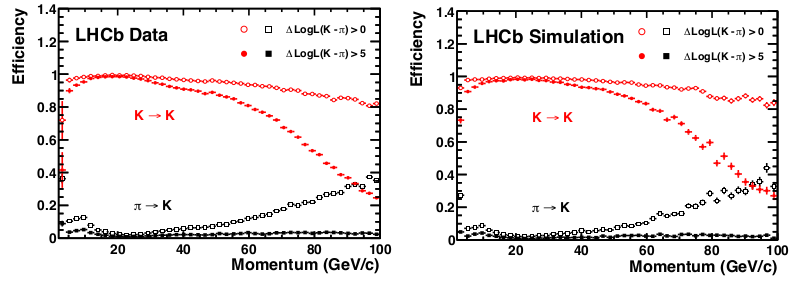
\includegraphics[scale=0.7]{figs/PID4.png}
\caption{Kaon identification efficiency and pion misidentification rate as meaured using data (left) and from simulation (right) as a function of track momentum~\cite{Aaij:2014jba}\red{improve}.\label{fig:PID4}}
\end{center}
\end{figure}

Finally, muons are identified in the muon system. The algorithm is based on the association of hits around its extrapolated trajectory. In this case, the logartihm of the ratio between the muon and non-muon (protons, pions and kaons)  hypothesis, $\Delta\log{\mathcal{L}(\mu)}$ is used as discriminating variable. Figure \ref{fig:PID5} shows, as a function of the track momentum and for different ranges of transverse momentum, the efficiency of the muon candidate selection, and the probabilities of incorrect identification of protons, pions and kaons as muons. 

\begin{figure} [htb!]
\begin{center}
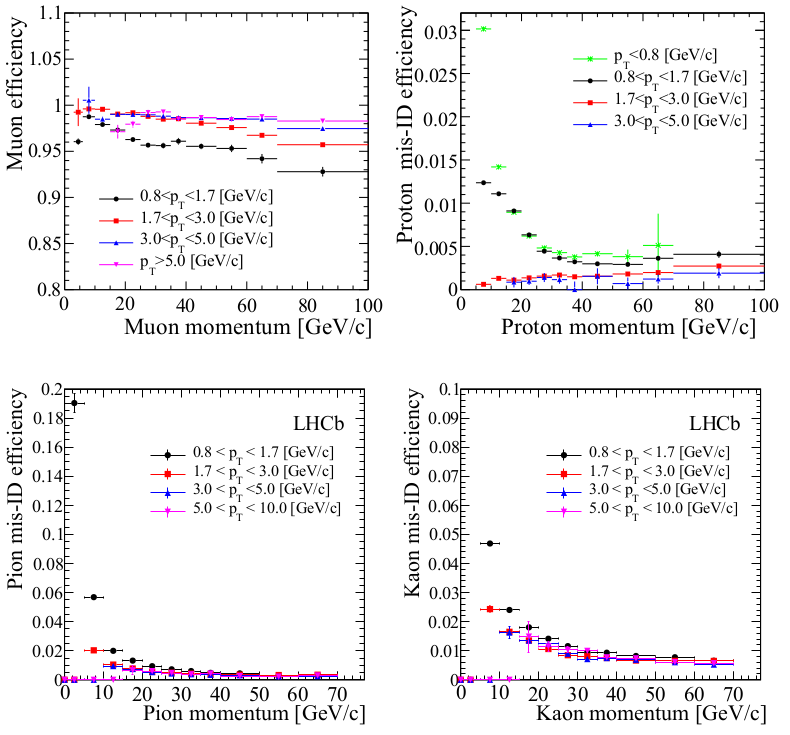
\includegraphics[scale=0.7]{figs/PID5.png}
\caption{Top left: efficiency of the muon candidate selection based on the matching of hits in the muon system to track extrapolation, as a function of momentum for different $p_T$ ranges. Other panels: msiidentification probability of protons (top right), pions (bottom left), and kaons (bottom right) as muon candidate as a function of momentum, for different $p_T$ ranges~\cite{Aaij:2014jba}.\label{fig:PID5}}
\end{center}
\end{figure}

The combined performance of the different PID subdetectors can be either be computed as a sum of the different likelihoods, or using multivariate techniques to get a single probabiity value for each particle hypothesis with different informations corresponding to each sub-system. 


\subsection{Trigger performance} %% 3 dias s2
\label{sec:TriggerPerformance}
As discussed in \ref{sec:Trigger}, the LHCb trigger is composed of two parts, in order to reduce the input rate to an output rate of 2 -5 kHz. The performance of each part is assessed using a data-driven technique with representative samples, to account for inefficiencies due to the simplified reconstruction algorithm, possible misalignments and reduced resolution. 

In the trigger system, an event is considered to be \textit{Trigger on Signal (TOS)} if the trigger objects that are associated with the signal candidate are sufficient to trigger the event. On the contrary, if the event has been triggered by trigger objectos not associated with the signal, it is considered \textit{Trigger Independet of Signal (TIS)}. Notice that events can be both TIS and TOS. The TIS and TOS efficiencies are defined as follows:
\begin{equation}
\epsilon^{\rm TIS(TOS)} = N^{\rm TIS \& TOS}/N^{\rm TOS(TIS)}
\end{equation}

\subsubsection{L0 hardware trigger}
The L0 trigger consists of three independent nits:
\begin{itemize}
\item The L0-Calorimeter trigger, that uses information from the SPD, PS, ECAL and HCAL to compute $E_T$ that particles deposit in clusters of 2x2 cells. From this, a candidate can be \texttt{L0Hadron}, \texttt{L0Photon} or \texttt{L0Electron}. 
\item The L0-Muon trigger, that looks for the two highest $p_T$ muon tracks in each quadrant, with thresholds on the $p_T^{\rm largest}$ and $p_T^{\rm largest} \times p_T^{\rm 2nd largest}$. 
\item The L0-PileUp trigger, used for the computation of the luminosity. 
\end{itemize}

Figure \ref{fig:L0Perf} shows the L0 hadron efficiency for the repreentative channels. As expected, it increases with the transverse momentum. 
\begin{figure} [htb!]
\begin{center}
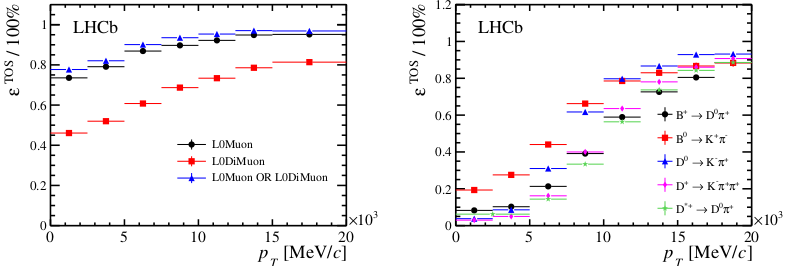
\includegraphics[scale=0.7]{figs/L0Perf.png}
\caption{(left) L0 muon trigger performance: TOS trigger efficiency for selected $B^+ \rightarrow J/\psi K^+$ candidates. (right) L0 hadron trigger performance: TOS trigger efficiency for different beauty and charm decay modes.~\cite{Aaij:2014jba}.\label{fig:L0Perf}}
\end{center}
\end{figure}


\subsubsection{High Level Trigger}
The HLT has a variety of so-called trigger "lines" that consist of selection parameters for specific classes of events. In HLT1, a partial event reconstruction is performed, while in HLT2 the complete event is reconstructed. 

In the first level (HLT1), vertices are reconstructed from a minimum of five intersecting VELO tracks. Vertices within a radius of 300 $\mu \rm m$ of the mean position of the pp-interaction envelope are considered to be primary vertices. During Run 1, the forward track search had a minimum momentum requirement that varied between 3 and 6 GeV/c. Dimuon candidates are either selected based on their mass without any displacement requirement, or based on theiir displacement without the mass restriction~\cite{}. The performance of HLT1 on muonic signatures as a function of $p_T$ of the $B^+$ parent is shown in \ref{fig:HLT1Perf}. 

\begin{figure} [htb!]
\begin{center}
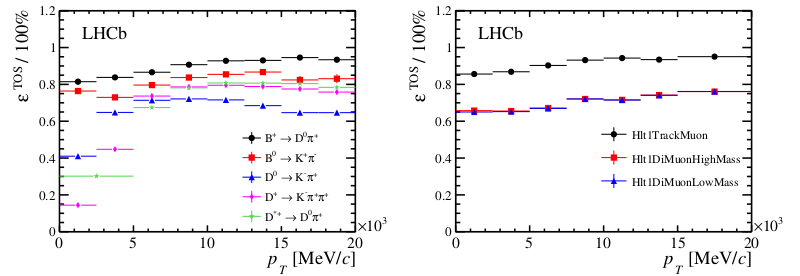
\includegraphics[scale=0.7]{figs/HLT1Perf.png}
\caption{HLT1 inclusive track trigger performance: TOS efficiency for various channels as a function of \textit{B} or \textit{D} $p_T$ (left) . HLT1 muon trigger performance : TOS efficiency for $B^+\rightarrow J/\psi K^+$~\cite{Aaij:2014jba}.\label{fig:HLT1Perf}}
\end{center}
\end{figure}


In the second level (HLT2), long tracks are searched based on VELO seeds, thus simplifying the offline tracking algorithm (because of CPU restrictions). There is a generic beauty trigger, for any partially recontructed \textit{b}-hadron decay, muon triggers, for decays with one or two muons, charm triggers and other exclusive and technical lines. Figure \ref{fig:HLT2Perf} shows the peformance of the $J/\psi$ triggers. %% comments? 

\begin{figure} [htb!]
\begin{center}
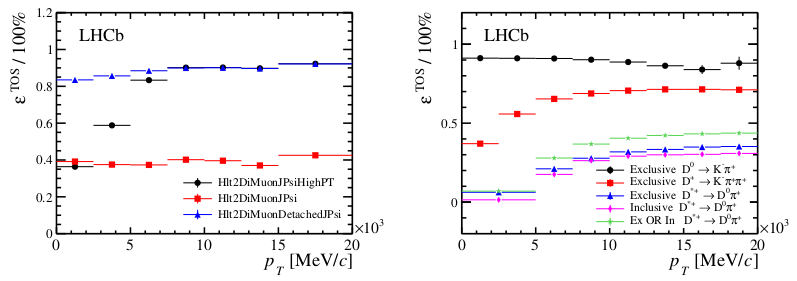
\includegraphics[scale=0.7]{figs/HLT2Perf.png}
\caption{HLT2 muon trigger performance for the $J/\psi$ trigger lines (left). HLT2 charm trigger performance for inclusive and exclusive selections (right).~\cite{Aaij:2014jba}.\label{fig:HLT2Perf}}
\end{center}
\end{figure}

%%\subsection{Experimental conditions} % jueves
%%% data, total luminosity

%%% magnetic field polarity 

\subsection{The LHCb Upgrade} % jueves, viernes, sabado

%%% Motivation: improve sensitivity, detector must be upgraded . fully exploit the potential of the LHC 
%%%update detector with read out at 40 MHz
%%% For this thesis 

The LHCb detector has proven to be an outstanding general-purpose detector in the forward pseudorapidity region. Nevertheless, some of the measurements are still statistically limited. Therefore, in order to fully exploit the potential of LHCb, an increase in the luminosity is required. This leads to the need of upgrading some of the subdetectors, since the upgraded detector is expected to collect 50 $\rm fb^{-1}$ during 5 years of data-taking, with a 40 MHz readout (Phase-I of the Upgrade).

For the sake of this thesis, the changes made during the LHCb Upgrade will greatly benefit the sensitivity to rare strange decays, as the trigger limitation will disappear. Also, a significant improvement in the $\phi_s$ measurement is expected. Prospects for the golden modes on these fields can be seen in \ref{fig:prospects}.

\begin{figure} [htb!]
\begin{center}
\includegraphics[scale=0.55]{figs/prospects.png}
\caption{Left: expected sensitivity for $\phi_s$ as a function of the luminosity. Right: Expected limit in $\mathcal{B}(K_S^0 \rightarrow \mu^+ \mu^-)$ from LHCb and upgrades, as a function of integrated luminosity times trigger efficiency.\label{fig:prospects} \red{refs}}
\end{center}
\end{figure}

\subsubsection{Trigger Upgrade} 
The main change that the LHCb trigger will undergo is the replacement of the L0 stage by a software one, the so-called \textit{Low Level Trigger} (LLT), modified to run within the new readout architecture. It selects events containing clusters with high transverse energy in the calorimeters or tracks with high transverse momentum in the muon detector. A much larger LLT rate will be alowed, leading to a much larger rate to storage. Hence, the main limits will be processing power and bandwith. The front-end electronics will be upgraded as well to allow reading events at the LHC clock rate. More details can be found in \red{REF}. 
\red{hadronic final states? (nota de Lars)}

%% Limits on processing power, bandwith
\subsubsection{VELO Upgrade} %%% jueves
The LHCb upgrade requires the VELO to have an excellent vertex resolution and two track separation, with fast pattern recognition capabilities. Moreover, because of the high luminosity, it has to have a sufficient radiation hardness to guarantee the performance throughout all the data-taking period. Besides, the upgraded trigger discussed before strongly relies on this subdetector. 

In order to cope with these requirements, two alternatives were  proposed:
\begin{itemize} 
\item A fine-pitched silicon strip detector, similar to the current design, with improved cooling and a new ASIC.
\item A hybrid pixel detector, called \textit{VeloPix}, that uses the Timepix chip \red{ref}. 
\end{itemize}
Being the latter the one chosen for the Upgrade. The layout of the upgraded VELO can be seen in \ref{fig:VELOUPGRADE}. 


\begin{figure} [htb!]
\begin{center}
\includegraphics[scale=0.7]{figs/VELO_Upgrade.png}
\caption{Schematic layout of the upgraded VELO.\label{fig:VELOUPGRADE}}
\end{center}
\end{figure}
 
\subsubsection{PID Upgrade}

As discussed before, the PID performance is crucial for the LHCb physics programme. Thus, its upgrade becomes of great importance. 

The overall structure of the RICH will remain unchanged. In RICH1, the aerogel will be removed, as the efficiency gained by its removal outweighs the improvement on the PID provided by it. The HPDs will be replaced by commercial multianode photomultipliers (MaPMTs), with external readout electronics. Alternatively a lens system may be used there, to re-focus the Cherenkov images onto the 1-inch tubes and thus reduce the number of tubes required. A new subdetector, still under development, is being considered in order to recover the low momentum particle identification performance. It consists in a time-of-flight system, Time Of internally Reflected Cherenkov Light, TORCH. 

As for the calorimeter, the electronics will be upgraded according to the new requirements. Also the PMTs \red{gains} will be reduced (and compensated by a gain increase in the electronics) to ensure a longer lifetime. Regarding the radiation hardness, studies have found the calorimeter resistent enough, even though some of the elements (such as the cells in the inner region of the ECAL) will need replacing in the long-term \red{scale}. Both the SOD and the PS will be removed, as they mainly contribute to the L0 trigger.

Finally, the muon system will have its first station removed, and additional shielding around the beam pipe in front of station M2. Similarly to the calorimeter, the electronics will be modified to comply with the new conditions. 

%An adaptation of the HPD, but with external readout electronics, is under study
%as an alternative photon detector.

\red{check}

\subsubsection{Tracking Upgrade} %% viernes
The TT stations will be replaced by a tracking detector composed of new, high-granularity silicon micro-strip planes with an improved coverage of the LHCb acceptance, the \textit{Upstream Tracker} (UT). Behind the magnet, a \textit{Scintillating Fibre Tracker} (SFT) will be built, which is composed of 2.5m long fibres read out by silicon photomultipliers at the edge of the acceptance, replacing the current OT and IT stations. Both new subdetectors can be seen in \ref{fig:LHCbUPGRADE}.

\begin{figure} [htb!]
\begin{center}
\includegraphics[scale=0.4]{figs/LHCb_upgrade.png}
\caption{Side view of the upgraded LHCb.\label{fig:LHCbUPGRADE}}
\end{center}
\end{figure}

%%% Subdetectors

\subsection{Analysis workflow}
%% rate of several million events per second, Gaudi,introduction to below
Raw data from collisions is taken at LHCb at a rate of several million events per second. A fast, efficient treatment and distribution of such data is thus needed to perform an offline analysis of a given decay channel. For this, C++ tools and algorithms embedded inside the Gaudi \red{ref} project are used. The steps that are followed, together with their correspondance to the different projects inside such framework, are summarised below. 

\begin{enumerate}
\item As explained in \ref{sec:Trigger}, \ref{sec:TriggerPerformance}, a first loose selection is applied to the recorded data with the trigger. The trigger algorithms constitute what is known as the Moore project \red{ref}. 
\item After data is recorded, it is necessary to convert the electronic signals to track and vertices. This was discussed in \ref{sec:Tracking} and \ref{sec:TrackingPerformance}. Particle identification (\ref{sec:PID}, \ref{sec:PIDPerformance}) is also required to properly assign each of these variables to a given type of particle. This whole process is called \textit{reconstruction}, and the group of C ++ LHCb libraries which contain the relevant tools, Brunel \red{ref}. Proper knowledge alignment of each subdetector is also of great importance at this stage, for which tools under the Alignment project \red{ref} exist.  %% reconstruction of tracks and vertices, PID (Brunel) alignment of each subdetector 
\item Once all triggered events have been reconstructed, a process is necessary to properly separate them offline according to their physics content. Such process, called \textit{stripping}, consists on a splitting procedure that selects the different decays according to their specific features (final state, PV, mother particle, etc.). Each of the selection criteria are contained in a \textit{stripping line}. The LHCb libraries that take part of this stage are DaVinci \red{ref} and Erasmus \red{ref}.
\item In order to allow the access to the data, while keeping a backup of it, a distributed system, \textit{Grid} \red{ref} is used by LHCb. Both stripped events and raw data are stored, so as to have the possibility of performing re-stripping and re-reconstruction if needed. Such system is of great computational power, and its spread in computing centers worlwide. 
\item Finally, to properly understand the effects from the detector and the steps before on data, simulation is used. Another important reason for which simulation is crucial is the need of training analysis tool on well-known states.
Simulated Monte Carlo events (MC) are employedfor this, mimicking as much as possible the data. The C++ libraries at LHCb dedicated to the MC production
are contained in Gauss \red{ref}, which is a collection of libraries for physics simulation based on Gaudi and with specialised algorithms and tools for generators (PYTHIA \red{ref}, EvtGen \red{ref}, ...) and detector simulation (Geant4 \red{ref}).
The MC events can be further classified as follows:
\begin{itemize}
\item Minimum Bias: keep all events generated by PYTHIA: elastic, diffractive, inelastic.
\item Inclusive: extract events generated by PYTHIA with at least one \textit{b} or \textit{c} hadron in 400 mrad with respect to the LHCb \textit{z} axis. If all of these hadrons have $p_z < 0$, flip the whole event.
\item Signal: extract events generated by PYTHIA containing at least one specific particle in 400 mrad. Again, if the candidate has $p_z < 0$, flip the whole event. In the case of \textit{b} hadrons and to speed up the generation, if the interaction contains the \textit{b}, repeat the hadronisation process of PYTHIA until the interaction contains the correct particle.
\end{itemize}
\end{enumerate}

\red{schematic view?}

		



\chapter{$\Delta \rm F$=2}
\label{sec:DF2}

\section{Introduction} %% 2 
%%% mixing amplitudes
The meson-antimeson ocillations are described by the mixing amplitudes~\cite{Altmannshofer:2009ne}
\begin{equation}
M_{12}^{(M)} \equiv \left \langle M | \mathcal{H}_{\rm eff}^{\Delta F = 2} | \bar{M} \right \rangle \ \, M = K^0, B_{d,s}
\end{equation}
%%% hamiltonian 
Where $\mathcal{H}_{\rm eff}^{\Delta F = 2}$ is the \textit{effective} Jamiltonian. Within the MSSM, it has the form:
\begin{equation}
\mathcal{H}_{\rm eff}^{\Delta F = 2}  = \sum_{i=1}^{5}C_i Q_i + \sum_{i=1}^{3}\tilde{C}_i\tilde{Q}_i + \rm h.c.
\end{equation}
with the operators $Q_i$ given, in the case of $B_s$ mixing, by:
\begin{equation}
\begin{split}
& Q_1 = (\bar{s}^{\alpha}\gamma_{\mu}P_Lb^{\alpha})(\bar{s}^{\beta}\gamma^{\mu}P_Lb^{\beta}) \\
& Q_2 = (\bar{s}^{\alpha}P_Lb^{\alpha})(\bar{s}^{\beta}P_Lb^{\beta}) \\
& Q_3 = (\bar{s}^{\alpha}P_Lb^{\beta})(\bar{s}^{\beta}P_Lb^{\alpha}) \\
& Q_4 = (\bar{s}^{\alpha}P_Lb^{\alpha})(\bar{s}^{\beta}P_Rb^{\beta}) \\
& Q_5 = (\bar{s}^{\alpha}P_Lb^{\beta})(\bar{s}^{\beta}P_Rb^{\alpha})
\end{split}
\label{eq:WOBs}
\end{equation}
where $P_{R,L} = \frac{1}{2}(1 \pm \gamma_5)$ and $\alpha,\beta$ are colour indices. The operators $\tilde{Q}_{1,2,3}$ are obtained from $Q_{1,2,3}$ by the replacement $L \leftrightarrow R$~\cite{Altmannshofer:2009ne}. In the case of $B_d$, the replacement $s \rightarrow d$ needs to be done in equation \ref{eq:WOBs}. 
Several representative observables can be extracted from these ampliudes, such as the mixing phase, the oscillation frequency or the semileptonic asymmetry:
\begin{equation}
\phi_s = \arg{(M_{12})}, \ \Delta m_s = |M_{12}|, \ A_{SL} = -\frac{\Delta\Gamma_s}{\Delta M_s} \tan{\phi_s}
\end{equation}
Note that their value strongly depends on NP contributions:
\begin{equation}
M_{12} = M_{12}^{SM} + M_{12}^{NP} 
\end{equation}
The experimental search of the weak mixing angle is discussed in detail in \ref{sec:phisEXP}. Theoretical interpretations \red{of this result} are reviewed in \ref{sec:phisPHEN}, and a \texttt{MultiNest} scan~\cite{Feroz:2008xx} is presented in \ref{sec:phisMULT}. 

\section{$\phi_s$ experimental} %% 10
\label{sec:phisEXP}

In the SM, \textit{CP}-violation originates from a single-phase in the Cabibbo-Kobayashi-Maskawa (CKM) quark-mixing matrix~\cite{Charles:2011va}, as explained in \ref{sec:CKMMatrix}. There are 3 different kinds of \textit{CP}-violation for neutral mesons, \textit{e.g.} $B_s^0$ and $\bar{B}_s^0$:
\begin{enumerate}
\item Direct \textit{CP}-violation: originated by a difference in the amplitudes associated to the direct decay of the $B_s^0$ and $\bar{B_s^0}$ mesons into the same final state %% CP eigenstate final 
\item \textit{CP}-violation in the $B_s^0- \bar{B}_s^0$ oscillation, that arises when the oscillation from $B_s^0$ to $\bar{B}_s^0$ is different from the oscillation from $\bar{B}_s^0$ to $B_s^0$
\item \textit{CP}-violation in the interference between the amplitudes  associated to the direct decay of a $B_s^0$ meson into a \textit{CP}-eigenstate final state and those associated to the decay after $B_s^0- \bar{B}_s^0$ oscillation
\end{enumerate} 
This last type of \textit{CP}-violation is characterized by the \textit{CP}-violating phase, $\phi_s$, defined as:
\begin{equation}
 \label{eq:phis}
\phi_s^f = -\rm arg(\lambda_f),\ \lambda_f = \eta_f \frac{q}{p}\frac{\bar{\mathcal{A}}_f}{\mathcal{A}_f},
\end{equation}
where \textit{f} is the final state, $\eta_f$ is 1(-1) for CP-even(CP-odd) states, $\left| \frac{q}{p} \right |$ determines the amount of \textit{CP}-violation in mixing, and ${\mathcal{A}}_f$($\bar{\mathcal{A}}_f$) is the amplitude of the $B_s^0$($\bar{B}_s^0$) meson decaying into a given final state, \textit{f}.
Precision measurements of this phase are needed in order to properly disentagle SM and NP contributions.

 In the SM, for $b\to c\overline{c}s$ transitions and ignoring subleading penguin contributions, this phase is predicted to be $-2\beta_s$, where $\beta_s=\arg\left[
 - (V_{ts} V_{tb}^*) / (V_{cs} V_{cb}^*)\right]$ and $V_{ij}$ are elements of the CKM quark flavour mixing
 matrix~\cite{Kobayashi:1973fv,Cabibbo:1963yz}. The indirect determination via global fits to experimental data gives
 \mbox{$2\beta_s=0.0364\pm0.0016\rad$}\red{~\cite{Charles:2011va}}. This precise indirect determination within the SM makes the
 measurement of $\phi_s$ interesting since new physics (NP) processes could modify
 the phase if new particles were to contribute to the $B_s^0$--$\bar{B}_s^0$\ box diagrams~\cite{Buras:2009if,Chiang:2009ev}.
 
\begin{figure}[h]
	\begin{center}
		\includegraphics[width=0.5\linewidth]{figs/Spring2017_Phis_vs_DGs.png}
	\end{center}
	\caption{\label{fig:HFAG}\small
		Individual 68$\%$ confidence-level contours of ATLAS, CMS, CDF, D0 and LHCb in the $(\phi_s^{c\overline{c}s},\Delta \Gamma_s)$, their combined contour (solid line  and shaded area), as well as the SM predictions (thick black rectangle) as performed by the HFLAV \cite{HFLAV2017} averaging group.
	}
\end{figure} 
 
The situation after including all Run 1 results from LHCb, and all results from ATLAS, CMS, CDF and D0 is shown in Figure~\ref{fig:HFAG}.
Current preliminary world averages (and their correlations) for the $CP$ violating phase $\phi_s$ and the decay width difference in the $B^0_s$ system, $\Delta \Gamma_s$, are:
\begin{eqnarray*}
\phi_s = -0.021 \pm 0.031\,\mathrm{rad} \\
\Delta \Gamma_s = 0.085 \pm 0.006\, \mathrm{ps}^{-1}\\
\rho( \phi_s ,  \Delta \Gamma_s ) =  -0.0095
\end{eqnarray*}

The aim of this analysis is to perform the measurement of $\phi_s$ in the \mbox{$B_s^0 \rightarrow J/\psi K^+ K^-$} channel by
adding a further $2\invfb$ of integrated luminosity collected at $13\tev$ in Run 2 of LHC in 2015 and 2016.
In addition, updated measurements of the decay width difference of the light (L)
and heavy (H) $B_s^0$ mass eigenstates,
$\Delta\Gamma_s \equiv \Gamma_{\mathrm L} - \Gamma_{\mathrm H}$, and the ratio between the
average widths in the $B_s^0$ and in the $B_d^0$ systems, $\Gamma_s/\Gamma_d$. 

\subsection{Phenomenology}
The baseline fit is obtained assuming that direct $CP$ violation caused by penguin diagrams is the same for all polarization states, therefore $\lambda_f$ is considered to be independent of the polarization state, $f$. Checks were made to check this ansatz. 

The theoretical differential decay rate for an initial $B_s^0$ as a function of decay time and angles using polarization dependent $\lambda_f = |\lambda_f|e^{-i \phi_s^f} \equiv |\lambda_f|e^{-i \phi_f} $ ($f=0,\,{||},\,{\perp},\,{\rm S}$) is given as~\cite{Liu:2013nea}
\begin{eqnarray}
 \frac{d^4 \Gamma( t) }{dm_{KK }^2 d\cos\theta_K d\cos\theta_l d\phi}&=&  \sum_{k=1}^{10} N_k h_k(t) f_k(\theta_K, \theta_l, \phi),  \label{eq:rate_mult_lambda}
 \end{eqnarray}
where the decay-time-dependent functions $h_k(t)$ are given as
\begin{eqnarray}
 h_k(t)= \frac{3}{ 4\pi}
   e^{-\Gamma t}\left\{ a_k \cosh\frac{\Delta \Gamma t}{2} + b_k \sinh\frac{\Delta \Gamma t}{2} + c_k \cos(\Delta mt)  +  d_k \sin(\Delta mt) \right\}.
\label{eq:rate_mult_lambda2}
\end{eqnarray}
For an initial $\bar{B}_s^0$ at production, the signs of $c_k$ and $d_k$ should be reversed. \red{appendix with coefficients?}
For the purpose of reducing correlation between fit parameters, it can be chosen to fit for $|\lambda_0|$, $\phi_0$ and $|{{\lambda_f}\over {\lambda_0}}|$, $\phi_f-\phi_0$, for $f \neq 0$.

\subsection{Samples and event selection}

In this section, the data and simulated samples used in this analysis are introduced, together with the trigger, stripping and offline selections applied to these samples.

\subsubsection{Data sample}

The analysis presented in this report uses a data sample collected at the LHCb
experiment at the LHC\@. The dataset corresponded to a total integrated
luminosity $\int{\mathcal{L}}{1.9 \rm fb^{-1}}$. Of this, $0.3 \rm fb^{-1}$ were taken in 2015 at a centre-of-mass energy $\sqrt{s}$ = 13$\rm TeV$ and $1.6 \rm fb^{-1}$ were taken in 2016 at $\sqrt{s}$ = 13$\rm TeV$.

Stripping version 26 was used for 2016 data and stripping version 24 was
used for 2015 data.  All stripping versions use exactly the same selection,
based on the {\tt StrippingBetaSBs2JpsiPhiDetached} {\tt
StrippingBetaSBd2JpsiKstDetached} and {\tt StrippingBetaSBu2JpsiKDetached} lines
in the DIMUON stream.  The data samples were processed using {\tt DaVinci} version
v42r1 and momentum scaling has been applied.

\subsubsection{Simulation samples}

In the LHCb simulation, $pp$ collisions are generated using
{\tt Pythia} with a specific \lhcb\ configuration~\cite{Sjostrand:2006za,
LHCb-PROC-2010-056}.

\begin{table}[h]
\begin{center}
\begin{tabular}{lcccc}
    \hline
    Event type & Decay mode & Options & Year & Events \\
    \hline
    \multicolumn{5}{c}{Signal modes}\\
    \hline
    13144004 & $\Bs\to\jpsi\phi$ & {\tt Update2012,dG=0,DecProdCut,S26} &  2016 & 25M \\
    13144011 & $\Bs\to\jpsi\phi$ & {\tt Update2016,DecProdCut,S26} & 2016 & 20M \\
    13144011 & $\Bs\to\jpsi\phi$ & {\tt Update2012,DecProdCut,S28} & 2016 & 10M \\
    13144011 & $\Bs\to\jpsi\phi$ & {\tt Update2016,DecProdCut,S24} & 2015 & XXM \\
    13144041 & $\Bs\to\jpsi\Kp\Km$ & {\tt DecProdCut} & 2016 & 7M \\
    %13100004 & $\Bs\to\jpsi\Kp\Km$ & {\tt Higher s-waves,DecProdCut} & 2016 & 20M \\
    \hline
    \multicolumn{5}{c}{Backgrounds}\\
    \hline
    15144001 & $\Lb\to\jpsi p\Km$    & {\tt PHSP, DecProdCut} &  XXX & XXM \\
    24142001 & Inclusive Jpsi & {\tt JpsiInAcc} &  2016 & 20M \\
    \hline
    \multicolumn{5}{c}{Control samples}\\
    \hline
    11144001 & $B^0 \to J/\psi K^{*0}$    & {\tt Update2016,DecProdCut,S24} & 2015  & 10M \\
    11144001 & $B^0 \to J/\psi K^{*0}$    & {\tt Update2016,DecProdCut,S26} & 2016  & 10M \\
    12143001 & $B^+ \to J/\psi K^+$    & {\tt Update2016,DecProdCut,S24} & 2015  & 10M \\
    12143001 & $B^+ \to J/\psi K^+$    & {\tt Update2016,DecProdCut,S26} & 2016  & 10M \\
    24142001 & Inclusive Jpsi & {\tt JpsiInAcc} &  2016 & 20M \\
    \hline
    \multicolumn{5}{c}{Generator Level}\\
    \hline
\end{tabular}
\caption{MC samples used in the analysis. SXX indicates the stripping version that is used to flag the events. DecProdCut means that all the daughters are required to be within LHCb acceptance.
}
\label{tab:mc}
\end{center}
\end{table}

Decays of hadronic particles are described by {\tt EvtGen}~\cite{Lange:2001uf}, in which final state radiation is generated using {\tt Photos}~\cite{Golonka:2005pn}. The {\tt Geant4} toolkit simulates the interaction of the generated particles with the detector, and the detector
response~\cite{Agostinelli:2002hh, Allison:2006ve}. Further details of the
simulation process can be found in Ref.~\cite{LHCb-PROC-2011-006}. The simulated data is processed in a very similar way to the real data, with the stripping run in flagging mode,
with no prescales applied for the trigger. Sim09b was used for the simulated samples.  The samples used are listed in Table~\ref{tab:mc}.

Simulated signal samples are used to determine the angular acceptance.  As will be discussed in Sec.~\ref{subsec:AngAcc}, the samples are reweighted to match various distributions observed in data before obtaining the final acceptance.  Similarly, the $\Lambda^0_b$ and the $B^0$ samples are used for background studies and decay time acceptance studies, respectively.  This is discussed in Sec.~\ref{subsec:MassFit} and Sec.~\ref{subsec:TimeAcc}, respectively.
The $B^+$ sample is used for tagging studies as described in Sec.~\ref{subsec:Tagging}.

The main physics parameters used in the main simulation used in this analysis, \texttt{Eventtype = 13144011, Bs\_Jpsiphi,mm=CPV,update2016,DecProdCut}, are summarized in Table~\ref{tab:evtgendecaypars13144011}. For simulated samples a momentum smearing is applied in order to reproduce better the distributions in data.

\begin{table}[h]
 \caption{\small Decay model parameters for the Sim09b MC sample used in this analysis, \texttt{Eventtype = 13144011, Bs\_Jpsiphi,mm=CPV,update2016,DecProdCut}.}
 \centerline{
   \begin{tabular}{cc}
      Parameter &       Value\\
     \hline
     $\Delta m_s$            & 17.8\invps \\
     $\Delta\Gamma_s$        & 0.08543\invps \\
     $\Gamma_s$              & 0.6614\invps \\
     $\phis$               & $-0.03$\rad  \\
     $|A_0(0)|^2$            & 0.5242 \\
     $|A_\|(0)|^2  $         & 0.2256  \\
     $|A_\perp(0)|^2  $       & 0.2500   \\
     $\delta_\|-\delta_0 $   & 3.26\rad  \\
     $\delta_\perp-\delta_0 $ & 3.08\rad \\\hline
   \end{tabular}}
 \label{tab:evtgendecaypars13144011}
\end{table}

\subsubsection{Stripping selection}

In order to select  $\Bs\to\jpsi\phi$ events, in data and MC we start from the stripping line {\tt StrippingBetaSBs2JpsiPhiDetachedLine}, whose selection can be found in Table \ref{tab:Bs2Jpsiphistripping}.
We use {\tt Stripping version 26} or {\tt 28} for 2016 and {\tt Stripping version 24} for 2015. In both cases the selection is the same.\\

 \renewcommand{\arraystretch}{1.2}
\begin{table}[h]
  \centering
  \caption{Selection criteria used to identify $B^0_s \to J/\psi \phi$ candidates.}
    \begin{tabular}{lrcc}\hline\hline
            &  Variable                        & Stripping \\
      \hline
      all tracks                       & $\chi^2_{\rm track}/{\rm nDoF}$                                & $<3$                     \\
       \hline
       $J/\psi \to \mu^{+} \mu^{-}$      &  $\Delta \mathrm{ln} \mathcal{L}_{{\mu}{\pi}}$ ($\mu^{\pm}$)   & $>0$                      \\
 			               &  $p_{T}$   ($\mu^{\pm}$)                                      & $>500\,\rm MeV/c$             \\
                                       & $\chi^2_{\rm DOCA}$                                           & $ < 20$                    \\
                                       & $\chi^2_{\rm vtx}/{\rm nDoF}$                                 & $ < 16$                    \\
               		               & $m(\mu^+\mu^-)$                                              &  $\in [3020,\,3170]\rm MeV/c^2$ \\
      \hline
      $\phi \to K^+ K^-$                & $\chi^2_{\rm DOCA}$                                           & $ < 30$                    \\
                                       &  $p_{T}$ ($\phi$)                                             & $>500\,\rm MeV/c$              \\
		                       & $m(K^+K^-)$                                                & $\in [980,\,1050]\rm MeV/c^2$                \\
                                       & $\chi^2_{\rm vtx}/{\rm nDoF}$                                 & $ < 25$                    \\
                                       & $\Delta \mathrm{ln} \mathcal{L}_{{K}{\pi}}$ $(K^+)$           & $>0$                          \\
      \hline
      $B^0_s \to \Jpsi \phi$           & $m(\jpsi\Kp\Km)$                                           & $\in [5150,\,5550]\mathrm{MeV/c^2}$  \\
                                       & $\chi^2_{\rm vtx}/{\rm nDoF}$                                 &  $< 20$  \\
                                       & $t$                                                          & $>0.2$ ps               \\
      \hline
    \end{tabular}
\label{tab:Bs2Jpsiphistripping}
\end{table}
\renewcommand{\arraystretch}{1.0}

For time resolution studies we use the stripping line {\tt BetaSBs2JpsiPhiPrescaledLine}, which has the same selection as shown in Table~\ref{tab:Bs2Jpsiphistripping} apart from the cut on the decay time of the $B^0_s$ candidate.

\subsubsection{Trigger selection}
\label{sec:trigger}

The following trigger strategy has been identified in order to retain the largest number of signal events while keeping a small number of trigger lines.
\begin{itemize}
\item No L0 requirements
\item HLT1 selection: {\tt Jpsi\_Hlt1DiMuonHighMassDecision\_TOS} or {\tt B\_Hlt1TrackMuonDecision\_TOS} or {\tt B\_Hlt1TwoTrackMVADecision\_TOS}
\item HLT2 selection: {\tt Jpsi\_Hlt2DiMuonDetachedJPsiDecision\_TOS}
\end{itemize}

\subsubsection{Corrections}
Corrections are applied to the simulated samples to match the distributions obtained from data:

\begin{enumerate}
        \item The stripped and triggered $B_s^0 \to J/\psi K^+K^-$ candidates are taken, with the $B_s^0$ decay time restricted to the range [0.3,15] ps. 
	\item The data invariant mass distribution of stripped and triggered $B_s^0 \to J/\psi K^+K^-$  candidates is fitted to obtain an sWeighted sample of data that is used in the following steps.
        %\item For MC, on top of the selection mentioned before only background categories 0 (signal), 50 (radiative events) with true decay time different from 0 and 60 (ghosts) are included (see Appendix~\ref{Appendix_BKGCAT} for a more detailed explanation).
        \item For MC, on top of the selection mentioned before only background categories 0 (signal) and 50 (radiative events) with true decay time different from 0 are included %%\red{more details?}.
	\item The simulation PID variable distributions are corrected using the {\tt PIDCalib} package.
	\item Using the above data sample, the $B_s^0$ production kinematics, nTracks distribution and the muon/kaon track ghost probability variables are reweighted.
\end{enumerate}

A BDT is trained to further improve the signal to background ratio. It is trained with 2016 samples. Namely, the 2016 corrected simulated sample for the signal sample while 2016 data candidates with $5450\rm MeV/c^2 < m(J/\psi K^+ K^-) < 5550\rm MeV/c^2$ are used
for the background sample.
Special care was taken to avoid variables that could introduce angular or decay time efficiencies, like impact parameter $\chi^2$ of final
state particles, the direction angle of the $B^0_s$ (DIRA) or transverse momentum of final state particles.
The figure of merit used to optimise the BDT response is given by
\begin{equation}
	{\rm FOM} = \frac{(\sum_i w_i)^2}{\sum_i w_i^2},
\end{equation}
where the index $i$ runs over all candidates in the sample and  $w_i$ are
per-candidate weights that are determined from the invariant mass fit
that is performed at each point in the scan over the BDT response. Figure~\ref{fig:FOM} shows on the left how the figure of merit performs and on the right the number of signal events divided by its uncertainty, both as a function of the BDT response. A similar distribution is observed. The optimal value is found to be at $> 0.78$.
After the BDT requirement has been applied there are
approximately 102\,000 signal candidates and 26\,000 background candidates
in the mass window of the fit, $5320\rm MeV/c^2 < m(J/\psi K^+ K^-) < 5420\rm MeV/c^2$ in 2016. The signal to background ratio is $\sim 3.9$. 
The mass fit used to determine sweights to statistically
remove this background and also the removal of peaking backgrounds for both 2015 and 2016 data samples is described in detail in the next \red{section}.

\begin{figure}[t]
	\begin{center}
    \includegraphics[width=0.49\linewidth]{figs/bs_2016_FOM}
		\includegraphics[width=0.49\linewidth]{figs/bs_2016_S_SIGMAS}
	\end{center}
	\caption{\label{fig:FOM}\small
		Distribution of the figure of merit used to optimise the cut on the BDT response (left) and distribution of signal yield divided by its uncertainty (right).}
\end{figure}

\subsection{Mass fit and computation of signal sWeights}
\label{subsec:MassFit}
The physics parameter of interest are extracted via a log-likelihood fit of the signal PDF to the unbinned decay time and anguar distributions. The events are first weighted to statistically subtract the background components using the \textit{sPlot} method~\cite{sWeights} with $m(J/\psi K^+ K^-)$ as the discriminating variable. 

In order to have an improved resolution, the $m(J/\psi K^+ K^-)$ is determined using both the $J/\psi$ mass and PV constraints. The combinatorial background is modelled with an exponential function and the signal distribution with a double-sided \textit{Crystal Ball} (CB) function. The double-sided CB function uses the per-event mass error as conditional observable, so that the correlation between $\cos{\theta_{\mu}}$ and mass resolution is taken into account. The full \textit{p.d.f} is the following: 

\begin{align*}
p &= N_{sig} CB(x;\mu,\alpha_1,\alpha_2,n_1,n_2,s_1,s_2 | \sigma_{i}) \\
&+ N_{bkg}((1-f_{B_d})e^{-\gamma_b x} + f_{B_d} Gauss(x;\mu_{B_d},\sigma_{B_d}),
\end{align*}
where $N_{sig}$ and $N_{bkg}$ is a number of signal and background events
correspondingly, $\mu$ is the mean of the distribution,
$s_1$ and $s_2$ are the scale factors, which accounts for underestimation of the per-event
mass error, $\alpha_1, \alpha_2, n_1, n_2$ are the tail parameters,
$\gamma_b$ is the coefficient in the exponential to describe the background.

The background sources that are considered consist in:
\begin{itemize}
\item $B^0 \rightarrow J/\psi K^{*0}$ peaking background, vetoed using PID cuts. 
\item $\Lambda_b^0 \rightarrow J/\psi pK^-$ peaking background, vetoed using PID cuts. The remaining events are statistically subtracted by injecting simulated events into the data tupe with a negative sum of weights equal to the expected number of events. 
\item $B^0 \rightarrow J/\psi K^+ K^-$ peaking background, modelled with a Gaussian in the nominal mass fit. 
\end{itemize}

For the fit to the $m(J/\psi K^+ K^-)$ distribution, the sample is divided
into twenty-four subsamples, each with an independent signal fraction and different
signal mass shapes. The subsamples correspond to six bins in the $K^+K^-$ mass,
namely [990, 1008, 1016, 1020, 1024, 1032, 1050] MeV/$c^2$, two trigger 
categories:
\begin{itemize}
\item \textbf{``Biased"}: {\tt B\_Hlt1TrackMuonDecision\_TOS} or {\tt B\_Hlt1TwoTrackMVADecision\_TOS} and not {\tt Jpsi\_Hlt1DiMuonHighMassDecision\_TOS} 
\item \textbf{``Unbiased"}: {\tt Jpsi\_Hlt1DiMuonHighMassDecision\_TOS}
\end{itemize}
and two years of the data-taking~(2015 and 2016). 

The event multipliciy (ratio between the number of events containing more than one cndidate and the total number of events) is found to be 1.2\% in the full $B_s^0$ mass region, but only 0.2\% for candidates in the signal region. Most of these candidates 
are due to cases where the $J/\psi$ is shared and one or two different kaons are added, making these events truly combinatorial in character. Given the low fraction of multiple events, it is evaluated as a systematic contribution removed them randomly. 

\subsection{\texorpdfstring{$C_{\rm SP}$}{Csp} factors}
\label{sec:CSP}
%LHCb-INT-2012-017
The relative change of the S-wave $m_{KK}$ line shape with respect to that of the P wave has to be considered in the interference terms of the angular expressions, as we are
performing the analysis in finite $m_{KK}$ bins (see Ref.~\cite{xie_CSP_sfiterror} for a detailed discussion). This is taken into account by adding a multiplicative correction factor, $C_{\rm SP}$, to the signal PDF, namely to the S-P-wave interference terms with $k=8,9,10$ in Eq. \eqref{eq:rate_mult_lambda}, i.e. $N_{k}\rightarrow C_{{\rm SP},i} N_{k}$. There are in total six  $C_{\rm SP}$ factors, one for each $m_{KK}$ bin.

The line shapes of the P and S wave are denoted as $p(m_{KK})$ and $s(m_{KK})$, respectively, where both are normalised to unity over a range $[m_{KK}^L,m_{KK}^U]$.
Essentially, the issue is that $\langle p\times s^*\rangle \neq \langle p \rangle \times \langle s^*\rangle$ in each $m_{KK}$ bin. Therefore, the product $p \times s^*$ is integrated, as it appears in the interference terms between the P and S wave. This yields

\begin{equation}
\label{eq:CSP}
\frac{\int_{m_{KK}^L}^{m_{KK}^H} { p \times s^*}  \:\:d m_{KK}}
{\sqrt{\int_{m_{KK}^L}^{m_{KK}^H} { |p|^2}  \:\:d m_{KK} \int_{m_{KK}^L}^{m_{KK}^H} { |s|^2}  \:\:d m_{KK}}}
 = C_{\rm SP} e^{-i \theta_{\rm SP}},
\end{equation}
where $C_{\rm SP}$ is the correction factor and the phase $\theta_{\rm SP}$ is
absorbed in the measurement of  $\delta_{\rm S} - \delta _{\perp}$.%phase space
model The shape of the P wave is a Breit-Wigner distribution, the same as in
Eq.(4) of Ref.~\cite{Liu:2241242}. The S-wave line shape is an $f_{0}$ with pole
mass of $0.9499$ GeV$/c^{2}$ as measured in Ref.~\cite{Liu:2241242}. Both the
$f_0$ and $\phi$ resonance distributions include a phase space factor $ \left (
\sqrt{\frac{P_B}{m_B}\frac{P_R}{\sqrt{s_{23}}}} \right )$, two Blatt-Weisskopf
factors for the \B and the $\Kp\Km$ resonance, and birth and decay momenta of
the $f_0, \phi$ and $\Bs$, where $L_B = 1, L_R = 0$ for $f_0$ and $L_B = 0, L_R
= 1$ for $\phi$. Note that the $f_0$ mass is considered to be 949 \mev. This
value, different from the PDG one ($990 \pm 30$ \mev)~\cite{PDG2017}, is taken
from the $\Bs\to\jpsi\pi^+\pi^-$ measurement~\cite{Aaij:2014emv}.

The detector reolution effect on the $C_{\rm SP}$ factors needs to be taken into account. While Eq.\ref{eq:CSP} is defined in dependence on the true $m_{KK}$, the mass bins are defined in dependence on the measured $m_{KK}$. The resolution effect can be incorporated as an efficiency correction, $\epsilon_i(m_{KK})$, of the $C_{\rm SP}$ factors
according to  
\begin{equation}
C_{SP} e^{-i \theta_{SP}} = \frac{\int_{2m_K}^{m_{B_s^0}-m_{J/\psi}} { p \times s^*\times \epsilon(m_{KK})}  \:\:d m_{KK}}{\sqrt{\int_{2m_K}^{m_{B_s^0}-m_{J/\psi}} { |p|^2\times \epsilon(m_{KK})} 
\:\:d m_{KK} \int_{2m_K}^{m_{B_s^0}-m_{J/\psi}} { |s|^2\times \epsilon(m_{KK})}  \:\:d m_{KK}}},
\label{eq:Csp2}
\end{equation}
\noindent where $\epsilon(m_{KK})$ is
\begin{equation}
\epsilon(m_{KK}) =
\begin{cases}
1, \text{ if $m_L< m_{KK} < m_H$} \\
0 \text{ otherwise}.
\end{cases},
\end{equation}
in the case where we bin in the true $m_{KK}$ mass (or equivalently, have perfect resolution). In reality though, we cut on a measured mass that has a finite resolution, and hence $\epsilon_{i}(m_{KK})$ will have a non-trivial structure. Note that in this definition we should consider events in the true $m_{KK}$ spectrum up to $2.27$ GeV/$c^{2}$, 
which is the value of $m_{B_s^0}-m_{J/\psi}$. However, the $\phi$ contribution after a certain point in $m_{KK}$ is too small to be modelled well in MC, so we apply an upper limit cut at $1.06$ GeV/$c^{2}$.
We use simulated events from the 2016 MC sample with and without S wave (see \tabref{tab:mc}) to determine $\epsilon_i(m_{KK})$ by dividing the $m_{KK}$ histogram before and after the selection of the events in each bin.
\figref{fig:epsilon_m} shows the corresponding distributions. We use the $C_{\rm SP}$ obtained from the MC without S wave with exception of the first bin, where the MC with S wave is used. The reason for this is that
in the region of $m_{KK}$, the contribution of the S wave is the largest and the MC with S wave has more events. With this, we obtain the $C_{\rm SP}$ factors shown in \tabref{tab:CSP1}.

\begin{figure}
\begin{center}
% \includegraphics[width=1.\textwidth]{figs/epsilon.pdf}
\includegraphics[width=0.49\textwidth]{figs/epsmKK.pdf}
\includegraphics[width=0.49\textwidth]{figs/epsmKK_SWave.pdf}
\caption{\small Efficiency of each \mKK bin selection as a function of MC true \mKK using MC without (left) and with (right) S wave.}
\label{fig:epsilon_m}
\end{center}
\end{figure}

\begin{table}[h]
        \caption{$C_{\rm SP}$ factors obtained using Eq.~\eqref{eq:Csp2}. The $\phi$ resonance is parametrized with a relativistic Breit-Wigner.}
        \begin{center}
        \begin{tabular}{c|c}
                                              & \multicolumn{1}{c}{S-wave line shape}\\
                                                \hline\\
%                 \mKK bin             & Spline S-wave&$f_0(980)$& Unsmeared $f_0(980)$ \\ \hline
                $m_{KK}$ bin             &$f_0$ \\ \hline
                1         	        & 0.8569 \\
                2                    & 0.8768  \\
                3                    & 0.8478  \\
                4                    & 0.8821  \\
                5                    & 0.9406  \\
                6                    & 0.9711  \\
        \end{tabular}
        \label{tab:CSP1}
        \end{center}
\end{table}

\subsection{Decay time resolution}
An effective single-Gaussian model is used to parametrize the decay time resolution. This is sufficient to describe the damping effect of the time resolution. It is defined as follows, % It also allowed for a simple determination of systematic uncertainties since no multiple correlated parameters need to be varied
\begin{equation}
    \mathcal{P}(t) = \mathcal{R}(t) \otimes
    \left[ f_{\mathrm{prompt}}\delta(t) + 
    f_{\mathrm{ll}} \left(f_{\mathrm{sl}}e^{- t / \tau_s} + (1 - f_{\rm sl})e^{- t / \tau_{\rm l}}\right)
    \right] + f_{\mathrm{wpv}} W(t),
    \label{eq:decay_time_pdf}
\end{equation}
Where $t$ is the decay time, $\delta_t$ the decay time uncertainty (both calculated from  decay tree fit in which the PV position is constrained without constraining the $J/\psi$ mass). This model is fitted to $t$ in ten bins of $\delta_t$, with ${\cal R}(t)$ being:
        \begin{equation}
            {\cal R}(t) \propto \sum_{i=1}^{3} f_i \frac{1}{\sqrt{2\pi}\sigma_i} e ^{-\frac{1}{2}\left(\frac{t-\mu}{\sigma_i}\right)^2},
        \label{eq:decay_time_res_model}
        \end{equation}
where $\sum_i f_i =1$.
The three Gaussians have a common mean, different widths and two relative fractions, which are allowed to vary in the fit, as are the lifetime and relative fractions of the exponential functions. Another component corresponding to events with a wrongly-associated PV is added, the fraction of which is allowed to float in the fit. In each bin of $\delta_t$, the dilution of the triple Gaussian model is computed as,
\begin{equation}
    \label{eqn:time_dilution_tr}
    D = \sum_{i=1}^{3}f_i e^{-\sigma_i^2\Delta m_s^2/2},
\end{equation}
and the effective single Gaussian width as,
\begin{equation}
    \label{eqn:time_eff_res_tr}
    \sigma_{\rm eff} = \sqrt{(-2/\Delta m_s^2)\ln D},
\end{equation}
where $\Delta m_s = 17.77 \rm ps^{-1}$. This converts the resolution into a single-Gaussian function with an effective resolution that causes the same damping effect on the magnitude of the $B_s^0$ oscillation. A linear or quadratic calibration curve is then fitted to the variation of the effective resolution as a function of $\langle\delta_t\rangle$ to determine the calibration parameters. 
%% Parameterization of the resolution model
For calibration, simulated $B_s^0 \rightarrow J/\psi \phi$, prompt $J/\psi$ and inclusive $J/\psi$ samples are used, as well as prompt $J/\psi$ data.
The main source of systematic uncertainty in the calibration of the decay time resolution model is the translation from the prompt background sample to the signal sample. In addition, there is a systematic arising from the choice to include or not the
wrong-PV component.

%%A simulated $B_s^0 \rightarrow J/\psi \phi$ sample is used as calibration. A quadratic dependence on $\delta_t$ is assumed for $\sigma_{\rm eff}$,
%\begin{equation}
%    \label{eqn:time_res_tr}
%    \sigma_{\rm eff}(\delta_t) = p_0 + p_1\langle\delta_t\rangle + p_2\langle\delta_t^2\rangle,
%\end{equation}
%being the fitted values of the calibration constants  $p_0 = 0.00810 \pm 0.00018 \rm ps$, $p_1 = 0.731 \pm 0.011$ and $p_2 = 3.29 \pm 0.15 \rm ps^{-1}$. This calibration corresponds to an effective (single-Gaussian) resolution of $40.96 \pm 0.03 \pm 0.04 \rm fs$ in the
%selected and background-subtracted $B_s^0 \rightarrow J/\psi \phi$ data sample, where the first uncertainty is statistical from the %size of the $B_s^0 \rightarrow J/\psi \phi$ data sample and the second from the uncertainties on the calibration parameters. % MC2015 + MC2016
%A calibration using the simulated inclusive $J/\psi$ sample yields a 0.1\% difference in $\sigma_{\rm eff}$ with respect to the former case. Such difference is asssigned as a systematic uncertainty on the decay time resolution coming from translating the resolution from the prompt sample to the signal sample.

\subsection{Angular acceptance}
\label{subsec:AngAcc}
The angular acceptance is modelled using \textit{normalization weights} (see Ref.~\cite{LHCb-ANA-2012-067}, Sec.~3.3) obtained from fully simulated signal events from the Sim09b production. This simulation sample is iteratively weighted to match the distributions of final-state particle kinematics in the real data, as well as to match the physics parameters obtained from data, in order to correct for imperfections in the detector simulation. In order to do this, a GB reweighting is first applied in $p(B_s^0)$, $p_T(B_s^0)$ and $m(K^+K^-)$, together with a reweighting in $p(K^{\pm})$, $p_T(K^{\pm})$. The angular normalizations are computed, and the process is repeated until convergence is achieved (after 4 iterations).  

A total of 10 normalization weights are computed for each year and trigger category, as indicated in table \ref{tab:angAccWeightsComb}, where the combined weights are shown. The factorization of angular acceptance and decay time acceptance is assumed. A systematic effect is assigned to such assumption, comparing the final acceptance normalization weights obtained in six equal populated decay time bins.

\begin{table}[hbtp]
 \caption{\small Angular acceptance weights determined from all available Monte Carlo samples. The $f_k$ are the normalizations of the angular functions (see Equation~\ref{eq:rate_mult_lambda}) including the acceptance. They are used in the normalization of the \textit{p.d.f.}} \label{tab:angAccWeightsComb}
 \center
\resizebox{\linewidth}{!}{
%\input{tex/AngAccTables/AngularAcceptanceTable_trigYearComp_2015_2016_IncldDG0_BKGCAT_0_50_60_sigmat015_XM_BP_BPT_KmpPTP_FirstKin_SepWeighting_16042018_fi__IncldG0_initial.tex}
\begin{tabular}{r l |c c c c}
\hline
& $k$ & \multicolumn{4}{c}{$f_k/f_1$}\\\hline
&     & \multicolumn{2}{c}{$2015$} & \multicolumn{2}{c}{$2016$} \\\hline
&     & ``Unbiased trigger"  & ``Biased" trigger & ``Unbiased trigger"  & ``Biased trigger"\\
\hline
1 & (00)                   &  $1  \pm 0$           &  $1\pm0$ & $1  \pm 0$           &  $1\pm0$ \\
2 & ($\parallel\parallel$) & $1.0297\pm0.0019$ & $1.0278\pm0.0036$ & $1.02637\pm0.00079$ & $1.0181\pm0.0017$\\
3 & ($\perp\perp$) & $1.0299\pm0.0019$ & $1.0280\pm0.0035$ & $1.02590\pm0.00078$ & $1.0184\pm0.0017$\\
4 & ($\parallel\perp$) & $-0.0007\pm0.0015$ & $-0.0071\pm0.0030$ & $-0.00029\pm0.00063$ & $0.0017\pm0.0015$\\
5 & ($0\parallel$) & $-0.00013\pm0.00090$ & $0.0038\pm0.0017$ & $0.00115\pm0.00038$ & $0.00260\pm0.00080$\\
6 & ($0\perp$) & $0.00119\pm0.00089$ & $0.0026\pm0.0017$ & $-0.00010\pm0.00038$ & $-0.00091\pm0.00079$\\
7 & (SS) & $1.0076\pm0.0013$ & $1.0123\pm0.0025$ & $1.00618\pm0.00054$ & $1.0112\pm0.0012$\\
8 & (S$\parallel$) & $-0.0005\pm0.0012$ & $-0.0008\pm0.0023$ & $0.00045\pm0.00048$ & $-0.0003\pm0.0010$\\
9 & (S$\perp$) & $-0.0008\pm0.0012$ & $0.0000\pm0.0023$ & $-0.00020\pm0.00049$ & $-0.0005\pm0.0010$\\
10 & (S0) & $0.0013\pm0.0024$ & $-0.0047\pm0.0047$ & $-0.0008\pm0.0010$ & $-0.0059\pm0.0022$\\
\hline
\end{tabular}
}
\end{table}
A cross-check has been performed using a sample of $B^+ \rightarrow J/\psi K^+$ decays in 2016 data, yielding a good consistency in the method. %% In this decay the muon helicity angle, $\theta$, exhibits a purely $\sin^2\theta$ dependence, which provides the benchmark against which the validity of the simulation can be tested. In particular, this study will investigate the behavior of the simulation correction as a function of $\eta(\Bu)$ since there are some issues with the performance of the simulation for charged tracks at low $\eta$.

\subsection{Decay time acceptance} 
\label{subsec:TimeAcc}
The reconstruction efficiency is not constant as a function of the $B^0_s$ decay time due to displacement requirements made on signal tracks in the trigger and event selection and to a decay-time-dependent efficiency to reconstruct the tracks in the VELO \cite{LHCb-PAPER-2013-065}. The overall decay-time acceptance is determined using the control channel $B^0 \to J/\psi K^{*}(892)^0$,
with $K^{*}(892)^0 \to K^+\pi^-$, which is kinematically very similar to the signal decay and it is assumed to have a purely exponential decay-time distribution with a well-known lifetime (i.e.the width difference $\Delta \Gamma_d$ is ignored), namely $1.518\pm 0.004$ ps\cite{HFLAV2017}.
The strategy to select $B^0 \to J/\psi K^{*}(892)^0$ events and compute the sWeights is similar to the one used for $B_s^0 \rightarrow J/\psi K^+ K^-$ events
The $K^+\pi^-$ system in the $B^0 \rightarrow J/psi K^+\pi^-$ decay can be in a relative S-wave or P-wave configuration. A $\sim6\%$ presence of S-wave has been observed in data, as described in~\cite{LHCb-PAPER-2013-023}. However, the simulated $B^0 \rightarrow J/\psi K^{*}(892)^0$ sample only includes the P-wave component. To account for this, an iterative procedure similar to the one described in \red{\ref{subsec:AngAcc}} is applied, reweigthing the simulation to match the $B^0$ $p$ and $p_T$, as well as $m(K^+\pi^-)$ distributions in data. %%\red{revisar}

The decay time acceptance is defined as
\begin{equation}
	\varepsilon_{\rm data}^{B_s^0}(t) = \varepsilon_{\rm data}^{B^0}(t) \times \frac{\varepsilon_{\rm sim}^{B_s^0}(t)}{\varepsilon_{\rm sim}^{B^0}(t)},
\label{eq:timeacc}
\end{equation}
where $\varepsilon_{\rm data}^{B^0}(t)$ is the efficiency in data of the fully triggered, selected and sweighted events in the $B^0$ control channel and $r(t)=\varepsilon_{\rm sim}^{B_s^0}(t)/\varepsilon_{\rm sim}^{B^0}(t)$ is the ratio of efficiencies of the
simulated signal and control modes after the full trigger, selection and MC-data correction chain has been applied.
This second term in the acceptance, $r(t)$, accounts for the small differences in the lifetime and kinematics between
the signal and control modes. The MC events are reweighted to match the $p.d.f.$ of the respective data. %%\red{more?} 

To derive $\varepsilon_{\rm data}^{B_s^0}(t)$ a simultaneous fit is performed to both the simultaneous samples and the data control channel. This allows to have the overall uncertainties on the $B^0_s$ data spline coefficients, thus providing an easier control on the associated systematic uncertainty. The decay time acceptance $\varepsilon_{\rm data}^{B_s^0}(t)$ is then used in the fit to the $B^0_s$ data signal sample to determine the physics parameters.

For the $B^0$ and $B_s^0$ the model used for the fit is composed of the product of a single exponential, convoluted with a single Gaussian resolution, and the respective acceptance function. The latter is modelled using cubic splines with knots at [0.3, 0.58, 0.91, 1.35, 1.96, 3.01,12.00] $\ps$ and the first coefficient is fixed to unity. The knot positions have been chosen according to an exponential distribution between [0.3,15] ps in order to have six equally populated bins considering $\Gamma=0.66\ps$. The last knot position is moved from 15 $\ps$ to 12 $\ps$ in order to have stable fits also for the trigger-year categories which have no decay candidates at these large decay times.

In order to obtain a single spline, $s_{data}^{B_s^0}$, that represents $\varepsilon_{\rm data}^{B_s^0}(t)$, combinations of the following three splines are used to describe the acceptance of the three datasets:
\begin{itemize}
\item One spline representing the acceptance in $B_s^0$ MC: $s_{sim}^{B_s^0}$
\item One spline representing the ratio of acceptances in $B^0$ and $B_s^0$ MC: $s_{sim}^{B^0/B_s^0}$
\item One spline representing the final acceptance in $B_s^0$ data: $s_{data}^{B_s^0}$
\end{itemize}
These splines are used in the following combinations to describe the acceptances for the three datasets:
\begin{itemize}
\item $B_s^0$ MC: $s_{sim}^{B_s^0}$
\item $B^0$ MC: $s_{sim}^{B^0/B_s^0} \times s_{sim}^{B_s^0}$
\item $B^0$ data: $s_{data}^{B_s^0} \times s_{sim}^{B^0/B_s^0}$
\end{itemize}

A single Gaussian models the resolution, and has a mean of 0$\rm ps$ and a width of 42$\rm fs$/39$\rm fs$/42$\rm fs$ for $B_s^0$ MC/$B^0$ MC/$B^0$ data, motivated by the studies in Section~\ref{sec:timereso} and the difference of the resolution between $B_s^0$ and $B^0$ seen in truth matched MC. The lifetime in the fit is fixed to the World average value for data $\tau_{B^0}^{\mathrm{data}} = 1.518\,\rm ps$~\cite{HFLAV2017}, and to the value used in the generation of the MC for the simulated samples, namely $\tau_{B^0}^{\mathrm{MC}} = 1.519\,\rm ps$ and $\tau_{\B^0_s}^{\mathrm{MC}} = 1.512\,\rm ps$.

The decay time acceptance is obtained separately for the data taking periods 2015 and 2016 and two different trigger paths (``unbiased" and ``exclusively biased"). 
\red{plots?}

The lifetimes $\tau(B^{0})$ and $\tau(B^{+})$ in $B^{0}\to \jpsi K^{*0}$ and $B^{+}\to \jpsi K^{+}$ decays are measured as a crosscheck of the time acceptance procedure. 2016 data and simulation samples for both validation channels are used.  The same procedure as for $B^{0}_{s}\rightarrow J/\psi \phi$ is used, including the spline knot positions and time resolution (see \secref{sec:timeAcc_timeaccBd}).

\subsubsection{Measurement of $\tau(B^{0})$} 

The procedure to determine the decay time efficiency (\secref{sec:timeAcc_timeaccBd}) is validated by splitting the 
$B^{0}\to\jpsi K^{*0}$ control sample (both data and simulation) into two independent sets. One half of the sample is then used as a control while the other is used to measure $\tau(B^0)$.
Three different criteria are considered for this, namely:
% Different splittings
\begin{itemize} 
    \item Splitting according to odd/even eventNumber in the
        original sample, where the sample that is used instead of $B_s^0$ has a
    cut on $\delta_t < 0.04\rm ps$.  
\item Splitting according to odd/even
        eventNumber in the original sample, where the sample that is used for
        fitting has a cut on the opening angle between the kaon and the pion
        that come from the $K^{*0}$, angle $<$ 0.025 rad. The position of the cut is
        chosen such that the average of the opening angle distribution is close
        to the corresponding one for the $B^{0}_{s}\to J/\psi \phi$ sample.
    \item Splitting on the $K^{*0}$ mass: events with $m(K^{*0}) < 890\ \rm
        GeV/{c^2}$ are used for fitting, events with $m(K^{*0}) > 890 \ \rm
        GeV/{c^2}$ are used as control sample.  
        \end{itemize}

For the control samples, the $B^{0}$ lifetime is fixed to its input for
simulation (1.519 ps) and to the
world average value for data (1.518 ps)~\cite{HFLAV2017}. We obtain the values
listed in the first column of \tabref{tab:tauB0}, where the deviation from the
world average ~\cite{HFLAV2017} is also shown. To
further improve these results, we also try reweighting the simulated samples according
such that the \Bd meson \pt distribution matches that in data,
as shown in \figref{fig:B0_PT_rew}.
The corresponding values for the lifetime (second column of \tabref{tab:tauB0})
show a better agreement with the PDG value. The fits to the decay time
distribution with MC reweighting in \pt for the different splittings are
shown in~\figref{fig:B0_tau_fit}.

Finally, a reweighting that takes into consideration the S-wave fraction present in
data (in addition to the aforementioned MC reweighting in $B^0$ \pt) is also
considered. %, using the results from Section~\ref{sec:Bd_swave}.
The splitting that is applied is the one depending on the $K^{*0}$
mass. The corresponding fitted lifetime is found to be  $\tau(\Bd) =
1.519\pm0.006$\ps, 0.13$\sigma$ (0.05\%) from the world average~\cite{HFLAV2017},
thus showing a good agreement. The fitted decay time is shown in
\figref{fig:B0_tau_fit}. 

\begin{table}[th]
\caption{\label{tab:tauB0}\small Values of $\tau(B^{0})$ obtained for validation of the time acceptance method for the different considered splittings, with (first column) and without reweighting MC in $p_{T}^{B}$.}
\centering{
\begin{tabular}{c|c|c}
    Splitting   & No $B^0$ $p_T$ reweighting & $B^0$ $p_T$ reweighting    \\
    \hline
   	$\delta_t < 0.04\rm ps$       & $1.482 \pm 0.007\rm ps$ (5.21$\sigma$,2.35\%)  & $1.518 \pm 0.007\rm ps$ (0.05$\sigma$,0.03\%)               \\ 
    angle $< 0.025\rm rad$     & $1.522 \pm 0.008\rm ps$ (0.52$\sigma$,0.28\%) & $1.523 \pm 0.008\rm ps$ (0.57$\sigma$,0.31\%)                  \\
    $m(K^{*0})$  & $1.518 \pm 0.006\rm ps$ (0.02$\sigma$,0.01\%) & $1.518 \pm 0.006\rm ps$ (0.03$\sigma$,0.01\%) 
\end{tabular}
}
\end{table}

% Plots with the reweighting 
\begin{figure}[tb!]
\centering{
    \includegraphics[width=0.29\textwidth]{figs/timeacc/B0_PT_reweighted_SigmaCut.pdf}
    \includegraphics[width=0.32\textwidth]{figs/timeacc/B0_PT_reweighted_AngleCut.pdf}
    \includegraphics[width=0.31\textwidth]{figs/timeacc/B0_PT_reweighted_MassCut.pdf}
	\caption{\small Distributions of $p_{T}^{B}$ for $B^{0}\to J/\psi K^{*0}$ using splitting according to eventNumber with $\sigma_t < 0.04$ (top left) and angle $<$ 0.025 (top right), and splitting according to $m(K^{*0})$ (bottom). The black dots represent data and the red and green lines the MC before and after the reweighting, respectively.
    \label{fig:B0_PT_rew}
        }}
\end{figure}

% Plots of the fit 
\begin{figure}[tb!]
\centering{
    \includegraphics[width=0.4\textwidth]{figs/timeacc/B0_time_fits_reweighted_SigmaCut.pdf}
    \includegraphics[width=0.4\textwidth]{figs/timeacc/B0_time_fits_reweighted_AngleCut.pdf}\\
    \includegraphics[width=0.4\textwidth]{figs/timeacc/B0_time_fits_reweighted_MassCut.pdf}
    \includegraphics[width=0.4\textwidth]{figs/timeacc/B0_time_fits_reweighted_MassCut.pdf}
	\caption{\small Decay time distribution of $B^{0}\to J/\psi K^{*0}$ decays and the corresponding
    likelihood fit result,
    splitting according to eventNumber with $\sigma_t < 0.04$ (top left) and angle $<$ 0.025 (top right), and splitting according to $m(K^{*0})$ without (bottom left) and with S-wave consideration.
    \label{fig:B0_tau_fit}
        }}
\end{figure}

%%\red{uncertainties}

\subsection{Flavour tagging}
\label{subsec:Tagging}
%%% Tagging parameters constrained in final fit → systematics propagated into final result
For time-dependent studies the ability of properly identifying the initial flavour of the meson (known as \textit{flavour tagging}) is fundamental. To this end, two flavour tagging algorithms are used: the opposite-side (OS) taggers and the same-side kaon (SSK) taggers, which exploit specific features of the incoherent production of $b\bar{b}$ quark pairs in $pp$ collisions.

Each tagging algorithm gives a tag decision and a mistag probability, the fraction of events with the wrong tag decision, $\eta \in [0, 0.5]$. The tag decision takes values +1, 1, or 0, if the signal meson is tagged as $B_s^0$, $\bar{B}_s^0$ or untagged, respectively. The fraction of events in the sample with a nonzero tagging decision gives
the efficiency of the tagger, $\varepsilon$. The mistag probability is then calibrated to obtain the corrected per-event mistag probability, $\omega$. This is used to determine the dilution factor, $\mathcal{D} = (1 − 2\omega)$, that rescales the efficiency of the tagger to quantify the fraction of the sample equivalent to perfectly tagged events. This effective efficiency is called tagging power, given by the product of the efficiency and the square dilution, $\varepsilon\mathcal{D}^2$.

In this analysis the taggers have been optimised for Run 1 data but here their
calibration is determined using Run 2 data. \red{update if necessary} A linear dependence of $\omega$ with $\eta$ is assumed, 
\begin{equation}
\omega = p_0 + p_1(\eta - \left \langle \eta \right \rangle)
\end{equation}
where $p_0$, $p_1$ are calibration parameters and $\left \langle \eta \right \rangle$ is the average predicted mistag probabilities for the calibration samples. When using OS and SSK algorithms, the calibration model become:
\\
\begin{center}
$\omega^{\rm alg} = (p_0^{\rm alg} + \frac{\Delta p_0^{\rm alg}}{2}) + (p_1^{\rm alg} + \frac{\Delta p_1^{\rm alg}}{2})(\eta^{\rm alg} - \left \langle \eta^{\rm alg} \right \rangle)$ for an initial $B_s^0$ event 
\end{center}
\begin{center}
$\omega^{\rm alg} = (p_0^{\rm alg} - \frac{\Delta p_0^{\rm alg}}{2}) + (p_1^{\rm alg} - \frac{\Delta p_1^{\rm alg}}{2})(\eta^{\rm alg} - \left \langle \eta^{\rm alg} \right \rangle)$ for an initial $\bar{B}_s^0$ event 
\end{center}
where $rm alg = OS, SSK$ and $\Delta p_i^{\rm alg}$ are mistag asymmetries. 

The calibration of the opposite-side tagger is made using $B^+ \rightarrow J/\psi K^+$ decays, while for the same-side kaon tagger $B_s^0 \rightarrow D_s^- \pi^+$ decays are used. The overall tagging performance is summarised in table \ref{tab:Tagging}. 

\begin{table}[h]
  \begin{center}
     \caption{Tagging performance}
  \label{tab:Tagging}
  \begin{tabular}{lcccc}
  \hline
    Category     & Fraction(\%) & $\varepsilon(\%)$  & $\mathcal{D}^{2}$   & $\varepsilon\mathcal{D}^{2}(\%)$ \\
    \hline                                                           
    OS-only  &14.44 & 10.26 & 0.087 & 0.90$\pm$0.03 \\ 
    SSK-only &59.48 & 42.28 & 0.030 & 1.29$\pm$0.31 \\ 
    OS\&SSK  &26.09 & 18.54 & 0.099 & 1.84$\pm$0.12 \\  
    \hline
    Total    &100  & 71.09 & 0.057 & 4.02$\pm$0.34 \\  
    \hline
  \end{tabular}
  \end{center}
\end{table}

\subsection{Data fitting}
The fitting procedure uses the sFit technique for background subtraction, as described in Section \ref{subsec:MassFit}.
The full PDF, based on Eq.~\eqref{eq:rate_mult_lambda} and taking into account all detector response effects, is given by
\small{
\begin{align}
 \!\!{\cal P}\left( t,\Omega| q^{\rm OS},  q^{\rm SSK}, \eta^{\rm OS}, \eta^{\rm SSK}, \sigma_{t} \right) = & 
 \sum_{y=2015}^{2016}\sum_{g=b,ub}\sum_{i=1}^{6}\sum_{k=1}^{10}\frac{1}{{\cal N}_{y,g}}{\cal P}_{i,k}\left( t,\Omega| q^{\rm OS},  q^{\rm SSK}, \eta^{\rm OS}, \eta^{\rm SSK}, \sigma_{t} \right) \nonumber \\
 = & \sum_{y=2015}^{2016}\sum_{g=b,ub}\sum_{i=1}^{6}\sum_{k=1}^{10} \frac{1}{{\cal N}_{y,g}}\tilde{N}_{i,k} f_{g,y,k}(\Omega)\varepsilon_{g,y}(t) \nonumber \\
 & \cdot \left\{\left[\left( 1+q^{\rm OS}\left(1-2\omega^{\rm OS}\left(\eta^{\rm OS}\right)\right)\right)
 \left(1+q^{\rm SSK}\left(1-2\omega^{\rm SSK}\left(\eta^{\rm SSK}\right)\right)\right)\right . \right .\nonumber \\
 & \;\;\;\;\cdot h_k\left(t | \Bs\right) \nonumber \\
 & +       \left .    \left(1-q^{\rm OS}\left(1-2\bar{\omega}^{\rm OS}\left(\eta^{\rm OS}\right)\right)\right)
\left(1-q^{\rm SSK}\left(1-2\bar{\omega}^{\rm SSK}\left(\eta^{\rm SSK}\right)\right)\right) \right.\nonumber \\
  & \;\;\;\;\cdot \left. h_k\left(t | \Bsb\right) \right] \otimes \left. G\left(t | \sigma_{t}\right) \right\},
 \label{eq:fullpdf}
 \end{align}}
where $i$ is the $m_{KK}$ bin; $y$ is the year of data taking; $g$ is the trigger line (biased and unbiased); $q^{\rm OS}$ and $q^{\rm SSK}$ are the OS and SSK tag decisions, $\eta^{\rm OS}$ and $\eta^{\rm SSK}$ the measured mistag probabilities, $\omega$ and $\bar{\omega}$ the mistag probability calibration for
$\Bs$ and $\Bsb$ (see Section~\ref{subsec:Tagging}); $\varepsilon(t)$ is the decay time acceptance (see Section~\ref{sec:timeacc}); $G\left(t | \sigma_{t}\right)$ is the decay time resolution with
decay time uncertainty $\sigma_{t}$ (see Section~\ref{sec:timereso}); $\tilde{N}_{i,k} = N_{k}$ for $k<8$ and $\tilde{N}_{i,k} = C_{{\rm SP},i}N_{k}$ for $k=8,9,10$ (see Section~\ref{sec:CSP}); 
${\cal N}_{y,g}$ is the normalisation given by
\begin{align}
 {\cal N}_{y,g}\left( t,\Omega| q^{\rm OS},  q^{\rm SSK}, \eta^{\rm OS}, \eta^{\rm SSK}, \sigma_{t} \right) = & 
 \int\displaylimits_{t=0.3\text{ps}}^{15\text{ps}}\int\displaylimits_{\Omega} \sum_{i=1}^{6} \sum_{k=1}^{10}w_{k} {\cal P}_{i,k}
 \left( t,\Omega| q^{\rm OS},  q^{\rm SSK}, \eta^{\rm OS}, \eta^{\rm SSK}, \sigma_{t} \right) dt d\Omega,
\end{align}
where $w_{k}$ are the angular acceptance weights (see Section \ref{sec:angular_acc}).

The values of $\phi_s$ and $\Delta \Gamma_s$ were kept blinded during the full analysis.%\red{rephrase}

\subsection{Baseline fit}
$\Delta\Gamma_d^s = \Gamma_s - \Gamma_d$ is fitted instead of $\Gamma_s$, given that it can be measured with a higher precision (independently of the value of $\Gamma_d$ used in the determination of the time acceptance). Events with negative mistag probability are manually assigned $\omega = 0$.
As said before, $\lambda$ and $\phi_s$ are assumed to be common to all polarisation states.  Checks of this assumption are made, where polarisation dependence is instead considered. These are in agreement with the baseline fit. 
Several fitters were independently developed, including the baseline one, based on the usage of graphics processing units (GPUs). These are optimized for parallel calculations that allow a faster computation. A good agreement is found between the fit results provided by the different fitters. 

The fit result is given in Table~\ref{tab:baselinefit} and the corresponding
correlation matrix in Table \ref{tab:fit_corr_matrix}.
The statisitical uncertainties reported are the symmetric uncertaintaies from Hesse\red{ref}. The background subtracted projection plots are shown in
Figures~\ref{fig:results_projections_time} and~\ref{fig:results_projections_angles}. 
One-dimensional likelihood profiles of the fit parameters are shown in Figures~\ref{fig:LikelihoodScans1}-\ref{fig:LikelihoodScans2}. \red{update} A summary of the systematic uncertainties is shown in \red{reference}. \ref{UPDATE WHEN FINAL}

\subsection{Coverage of the uncertainty with the sFit}

To check the reliability of the uncertainties on the physics parameters in the data fit to the time and helicity angles, the method of bootstrapping is applied to both data and simulation. For this, a set of pseudo-samples is created by randomly selecting events from the simulation or data sample. The number of events in each pseudo-sample is the same as the number of events of the original one. 
After creating the samples, they are fitted, and the central value and pull distributions for each fit parameter are plotted (see figures in Appendix~\ref{app:Bootstrapping}). The corresponding  bootstrapping uncertainty (and the uncertainty on the uncertainty) for each parameter is obtained from the RMS of the distribution of its central values.

\subsubsection{Simulation}
\label{sec:boostr_MC}
The results for bootstrapping using simulation are shown in \tabref{tab:BootstrappingMC}. For this study a simulation sample from 2016 has been used, with \texttt{S26} applied. Good agreement is found between the errors provided by the fit and the ones computed using bootstrapping.

\begin{table}[h]
        \caption{\small Variation in the statistical uncertainties for the fit parameters using the errors provided by the fit and the ones obtained with bootstrapping for simulation.}
\begin{center} % (Q) More digits?
   \begin{tabular}{c c c}
        Parameter & Fit  & Bootstrapping   \\ \hline
        $f_L$ & 0.0006  & 0.0005819  $\pm$  0.000002
 \\
        $f_\perp$  &  0.0008 & 0.000796  $\pm$  0.0000126
 \\
        $\phi_s$ [\rad] $^*$  & 0.0016 & 0.0016091  $\pm$ 0.0000256
 \\
         $\delta_\perp $ [\rad] & 0.006  & 0.0063273  $\pm$  0.0001005
 \\
         $\delta_\parallel$ [\rad] & 0.007  & 0.006711  $\pm$  0.0001066
 \\
         $\left | \lambda \right |$ & 0.001 & 0.0010967  $\pm$  0.0000174
 \\
         $\Delta\Gamma^s_d$ [\invps] & 0.0005 & 0.00057  $\pm$  0.0000091
 \\
         $\Delta\Gamma_s$ [\invps]$^*$ & 0.0016 & 0.0015527  $\pm$  0.0000247
 \\
         $\Delta ms$ [\invps]  & 0.0021 & 0.0021915  $\pm$  0.0000348
 \\
 \end{tabular}
 \label{tab:BootstrappingMC}
\end{center}
\end{table}

\subsubsection{Signal and background simulation}
A sample composed by signal and background is used for the bootstrapping studies. It is obtained using a \texttt{S28}, 2016 simulation sample, combined with background that is 
generated from 2016 data's sidebands. The preliminary results are shown in \tabref{tab:BootstrappingMCwBkg}. Results for the nominal fit are shown in \tabref{tab:FitMCwBkg}, together with the corresponding inputs used for MC. As for the test with pure signal MC (see Sec.~\ref{sec:boostr_MC}), good agreement is found between the errors obtained using bootstrapping and the ones provided by the fit. 

\begin{table}[h]
        \caption{Variation in the statistical uncertainties for the fit parameters using the errors provided by the fit and the ones obtained with bootstrapping for signal and background simulation.}
\begin{center} % (Q) More digits?
   \begin{tabular}{c c c}
        Parameter & Fit  & Bootstrapping   \\ \hline
        $f_L$ & 0.0008834  & 0.0008598  $\pm$  0.0000118
 \\
        $f_\perp$  & 0.001239 & 0.0012018  $\pm$  0.0000165
 \\
        $\phis$ [\rad] $^*$  & 0.009296 & 0.0094382  $\pm$  0.0001296
 \\
         $\delta_\perp $ [\rad] & 0.03491 & 0.036471  $\pm$  0.0005006 
 \\
         $\delta_\parallel$ [\rad] & 0.0289 & 0.0239876  $\pm$  0.0003292
 \\
         $\left | \lambda \right |$ & 0.006291 & 0.0062407  $\pm$  0.0000857 
 \\
         $\Delta\Gamma^s_d$ [\invps] & 0.0007465 & 0.0007257  $\pm$  0.000010
 \\
         $\DGs$ [\invps]$^*$ & 0.002395 & 0.0022637  $\pm$  0.0000311
 \\
         $\dms$ [\invps]  & 0.01379 & 0.0144994  $\pm$  0.000199 
 \\
 \end{tabular}
 \label{tab:BootstrappingMCwBkg}
\end{center}
\end{table}

\begin{table}[h]
        \caption{Fit results for signal and background simulation}
\begin{center} % (Q) 
   \begin{tabular}{c c|c}
        Parameter & Fit  & Input   \\ \hline
        $f_L$ & 0.5288 $\pm$ 0.0008834 & 0.5241
 \\
        $f_\perp$  & 0.247 $\pm$ 0.001239 & 0.25
 \\
        $\phis$ [\rad] $^*$  & -0.04027 $\pm$ 0.009296 & -0.03
 \\
         $\delta_\perp $ [\rad] & 3.042 $\pm$ 0.03491 & 3.08 
 \\
         $\delta_\parallel$ [\rad] & 3.23 $\pm$ 0.0289 & 3.26
 \\
         $\left | \lambda \right |$ & 0.9988 $\pm$ 0.006291 & 1.0 
 \\
         $\Delta\Gamma^s_d$ [\invps] & 0.005276 $\pm$ 0.0007465 & 0.00601 
 \\
         $\DGs$ [\invps]$^*$ & 0.08673 $\pm$ 0.002395 & 0.0854
 \\
         $\dms$ [\invps]  & 17.8 $\pm$ 0.01379 & 17.8
 \\
 \end{tabular}
 \label{tab:FitMCwBkg}
\end{center}
\end{table}

\subsubsection{Data}
The results for bootstrapping using 2016 data can be seen in \tabref{tab:BootstrappingData}. In this case, sWeighted 2016 data has been used, with Stripping version 26.  Contrary to simulation, discrepancies are found between bootstrapping and fit errors, especially in the strong phases and the S wave fit fractions. There could be a couple of
possible explanations for this. First, the sWeights used for the fit are not recalculated for each randomly drawn sample, which can lead to differences in the uncertainties.
However, this doesn't seem to affect the MC and so is probably only a secondary effect. Second, the bootstrapping test shows two minima for $\delta_S^1 - \delta_\perp$. A likelihood profile test on the data confirmed this. A reliable error estimation for the lower minimum is impossible because it merges with the higher minimum before the likelihood  changes by a significance of $1\sigma$. Last but not least, the likelihoods of some parameters show an asymmetric and non-Gaussian behaviour. This is especially true for the S wave parameters, where the fit fractions are low and we lack the statistical power to determine their uncertainties. In these cases, the fit errors are not an apt estimate of the  uncertainties. Instead, for the final result the uncertainties will be taken from the parameter likelihood profiles.

\begin{table}[h]
        \caption{ Variation in the statistical uncertainties for the fit parameters using the errors provided by the fit and the ones obtained with bootstrapping for 2016 data.}
\begin{center} % (Q) More digits?
   \begin{tabular}{c c c}
        Parameter & Fit  & Bootstrapping   \\ \hline
        $f_L$ & 0.003124  & 0.0032169 $\pm$  0.0000474
 \\
        $f_\perp$  & 0.0043  & 0.0043788 $\pm$ 0.0000645
 \\
        $\phis$ [\rad] $^*$ & 0.04637 & 0.0474420 $\pm$  0.0006984
 \\
         $\delta_\perp$ [\rad] & 0.1304  & 0.1492076 $\pm$  0.0021966
 \\
         $\delta_\parallel$ [\rad] & 0.07729  & 0.0414571  $\pm$  0.0006103
 \\
         $\left | \lambda \right |$ & 0.01579  & 0.0191426  $\pm$  0.0002818
 \\
         \red{$\Gamma_s$ [\invps]} & 0.002529 & 0.0025023 $\pm$ 0.0000368
 \\
         $\DGs$ [\invps]$^*$ & 0.008355 & 0.0082595 $\pm$  0.0001216
 \\
         $\dms$ [\invps] & 0.05667 & 0.0733526  $\pm$  0.0010799
 \\
          $\delta_S^1 - \delta_\perp$ & 0.3492 & 0.6728437 $\pm$  0.0099055
 \\
         $\delta_S^2 - \delta_\perp$ & 0.3653  & 0.3101728  $\pm$  0.0045663
 \\
         $\delta_S^3 - \delta_\perp$ & 0.4979 & 0.4256790 $\pm$  0.0062668
 \\
         $\delta_S^4 - \delta_\perp$ & 0.1823 & 1.6134152 $\pm$  0.0237524
 \\
         $\delta_S^5 - \delta_\perp$ & 0.1006 & 0.4099490 $\pm$  0.0060352
 \\
         $\delta_S^6 - \delta_\perp$ & 0.1935 & 0.2751857 $\pm$  0.0040512
 \\
         $F_S^1$         & 0.04565 & 0.0477817 $\pm$  0.0007034
 \\
         $F_S^2$         & 0.00963 & 0.0094324 $\pm$  0.0001389
 \\
         $F_S^3$         & 0.002055 & 0.0020870 $\pm$  0.0000307
 \\
         $F_S^4$         & 0.005845 & 0.0054945 $\pm$  0.0000809
 \\
         $F_S^5$         & 0.01386 & 0.0144309 $\pm$  0.0002124
 \\
         $F_S^6$         & 0.02029 & 0.0201681 $\pm$  0.0002969
 \\
 \end{tabular}
 \label{tab:BootstrappingData}
\end{center}
\end{table}

\red{combination with run 1?}

\section{$\phi_s$ pheno} %% 10
\label{sec:phisPHEN}
\red{
\begin{enumerate}
\item Introduction
\item WCs 
\item Plots
\item Scan ranges
\item Interpretation 
\end{enumerate}
}

%%%%%%%%%%%%%%%%%%%%%%%%%%%%%%%%%%%%%%%%%%%%%%%%%%%%%%
\subsection{Observables}
%%%%%%%%%%%%%%%%%%%%%%%%%%%%%%%%%%%%%%%%%%%%%%%%%%%%%%
\begin{table}[!t]
\begin{center}
\begin{tabular}{c@{\hspace{0.05\textwidth}}c}
Observable & Constraint \\
\hline
$\Delta M^{\rm EXP/SM}_{s}$ & $  0.968 \pm 0.078$ \red{TK: $ 
0.887(59) [1712.06572]$} \\ 
$\phi_s - \phi_s^{SM}$ &  $0.0154 \pm 0.031$\\ 
$\mathcal{B}(B_s^0 \rightarrow \mu^+ \mu^-)^{\rm EXP/SM}$ & $0.9 \pm 0.2(\rm EXP) \pm 0.1(\rm TH)$\\
$\mathcal{B}(B_d^0 \rightarrow \mu^+ \mu^-)^{\rm EXP/SM}$ & $4.0 \pm 2.0(\rm EXP) \pm 0.4(\rm TH)$\\
$\Delta m_s A_{SL}/\Delta \Gamma_s - (\Delta m_s A_{SL}/\Delta \Gamma_s)^{SM}$ & $-0.1258 \pm 0.5651$\\
$\mathcal{B}(B^+ \rightarrow \tau^+ \nu_{\tau})^{\rm EXP/SM}$ & $0.91 \pm 0.22$~\cite{Patrignani:2016xqp} \\ 
$\Delta C_7 $ & $-0.02 \pm 0.02$~\cite{C7_constraints} \\ 
$m_H$ & $125.09 \pm 20 \ \rm [GeV]$  \red{[2016 PDG]}\\
$\tan\beta$:$M_{A}$ plane & ATLAS limits for hMSSM scenario~\cite{Aaboud:2017sjh} \\
LSP & Lightest neutralino \\
\hline
\end{tabular}
\end{center}
\caption{\label{tab:Observables}Physics observables constraints imposed in this study.}
\end{table}


\section{$\phi_s$ \texttt{MultiNest}} %% 8 7
\label{sec:phisMULT}
A scan is performed using the \texttt{MultiNest} Bayesian inference tool~\cite{Feroz:2008xx}, with \textcolor{blue}{2016 LHCb data}. More details on the MultiNest algorithm are given in the following subsection. 
%%% beginning of bullshit:
The lower and upper bins are removed from the scan, as they represent a high computational cost and they don't have much statistics. Therefore, only 4 $m_{KK}$ bins are used. To this same end, $\Gamma_s - \Gamma_d$ is fixed to \red{its PDG value}, -0.002678 $\rm ps^{-1}$. 
The results are shown in figures~\ref{fig:phisMN1D} and ~\ref{fig:phisMN2D}. As it can be seen from these, the scan results are in agreement with the fit results. Moreover, two minimas for positive and negative $\Delta\Gamma_s$ are shown. \red{...}
%%% end of bullshit

%%%%%%%%%%%%%%%%%%%%%%%%%%%%%%%%%%%%%%%%%%%%%%%%%%%%%%%%%%%%%%%%%%%%%%%%%%%%%%%%%%
%%%%%%%%%%%%%%%%%%%%%%%%%%%%%%%%%%%%%%%%%%%%%%%%%%%%%%%%%%%%%%%%%%%%%%%%%%%%%%%%%%
%%%%%%% Beginning of placeholder:
\begin{center}
\includegraphics[width=0.49\textwidth]{figs/DG.png}
\includegraphics[width=0.49\textwidth]{figs/Dm.png}\\
\includegraphics[width=0.49\textwidth]{figs/lambda_0_abs.png}
\includegraphics[width=0.49\textwidth]{figs/phis_0.png}\\
\includegraphics[width=0.49\textwidth]{figs/fL.png}
\includegraphics[width=0.49\textwidth]{figs/fpe.png}\\
\includegraphics[width=0.49\textwidth]{figs/dpa.png}
\includegraphics[width=0.49\textwidth]{figs/dpe.png}\\
\includegraphics[width=0.49\textwidth]{figs/Fs_2.png}
\includegraphics[width=0.49\textwidth]{figs/Fs_3.png}\\
\includegraphics[width=0.49\textwidth]{figs/Fs_4.png}
\includegraphics[width=0.49\textwidth]{figs/Fs_5.png}\\
\includegraphics[width=0.49\textwidth]{figs/ds_m_dpe_2.png}
\includegraphics[width=0.49\textwidth]{figs/ds_m_dpe_3.png}\\
\includegraphics[width=0.49\textwidth]{figs/ds_m_dpe_4.png}
\includegraphics[width=0.49\textwidth]{figs/ds_m_dpe_5.png}\\
\label{fig:phisMN1D}
\end{center}

\begin{center}
\includegraphics[width=0.49\textwidth]{figs/DG_vs_Dm.png}
\includegraphics[width=0.49\textwidth]{figs/DG_vs_dpa.png}\\
\includegraphics[width=0.49\textwidth]{figs/DG_vs_dpe.png}
\includegraphics[width=0.49\textwidth]{figs/DG_vs_fL.png}\\
\includegraphics[width=0.49\textwidth]{figs/DG_vs_dpa.png}
\includegraphics[width=0.49\textwidth]{figs/DG_vs_fpe.png}\\
\includegraphics[width=0.49\textwidth]{figs/DG_vs_lambda_0_abs.png}
\includegraphics[width=0.49\textwidth]{figs/DG_vs_phis_0.png}\\
\includegraphics[width=0.49\textwidth]{figs/Dm_vs_dpa.png}
\includegraphics[width=0.49\textwidth]{figs/Dm_vs_dpe.png}\\
\includegraphics[width=0.49\textwidth]{figs/Dm_vs_fL.png}
\includegraphics[width=0.49\textwidth]{figs/Dm_vs_lambda_0_abs.png}\\
\includegraphics[width=0.49\textwidth]{figs/dpa_vs_fL.png}
\includegraphics[width=0.49\textwidth]{figs/Dm_vs_phis_0.png}\\
\includegraphics[width=0.49\textwidth]{figs/dpe_vs_dpa.png}
\includegraphics[width=0.49\textwidth]{figs/dpe_vs_fL.png}\\
\includegraphics[width=0.49\textwidth]{figs/fpe_vs_Dm.png}
\includegraphics[width=0.49\textwidth]{figs/fpe_vs_dpa.png}\\
\includegraphics[width=0.49\textwidth]{figs/fpe_vs_dpe.png}
\includegraphics[width=0.49\textwidth]{figs/fpe_vs_fL.png}\\
\includegraphics[width=0.49\textwidth]{figs/fpe_vs_lambda_0_abs.png}
\includegraphics[width=0.49\textwidth]{figs/fpe_vs_phis_0.png}\\
\includegraphics[width=0.49\textwidth]{figs/lambda_0_abs_vs_dpa.png}
\includegraphics[width=0.49\textwidth]{figs/lambda_0_abs_vs_dpe.png}\\
\includegraphics[width=0.49\textwidth]{figs/lambda_0_abs_vs_fL.png}
\includegraphics[width=0.49\textwidth]{figs/phis_0_vs_dpa.png}\\
\includegraphics[width=0.49\textwidth]{figs/phis_0_vs_dpe.png}
\includegraphics[width=0.49\textwidth]{figs/phis_0_vs_fL.png}\\
\includegraphics[width=0.49\textwidth]{figs/phis_0_vs_lambda_0_abs.png}
\label{fig:phisMN2D}
\end{center}

%%%%%%%%%%%%%%%%%
%%%%%%%%%%%%%%%%%%%%%%%%%%%%%%%%%%%%%%%%%%%%%%%%%%%%%%%%%%%%%%%%%%%%%%%%%%%%%%%%%%
%%%%%%%%%%%%%%%%%%%%%%%%%%%%%%%%%%%%%%%%%%%%%%%%%%%%%%%%%%%%%%%%%%%%%%%%%%%%%%%%%%

\red{
\begin{enumerate}
\item Description of the tool
\item Description of the plots + Methodology
\item Conclusions from the plots 
\end{enumerate}
}

\subsection{\texttt{MultiNest}}
\ref{sec:MultiNest}
\texttt{MultiNest} is a multimodal, parallelizable nested sampling algorithm. 

It calculates the evidence, with an associated error estimate, and produces posterior samples from distributions that may contain multiple modes and/or pronounced (curving) degeneracies in high dimensions. The algoritm also naturally identifies individual modes of a distribution, allowing for the evaluation of the 'local' evidence and parameter constraints associated with each mode separately.
%%It outperforms \red{in efficiency and robustness} the existing Markov chain Monte Carlo (MCMC) sampling, used for parameter estimation. This can be computationally intensive, and often experience problems in sampling efficiently from a multimodal posterior distribution or one with large (curving) degeneracies between parameters, particularly in high dimensions. Besides, MCMC methods often require careful tuning of the proposal distribution, and testing for convergence can be problematic. %%% The existing preferred evidence evaluation method, again based on MCMC techniques, is thermodynamic integration (greater computational expense to compute the key ingredient, the Bayesian evidence)
%% Bayesian evidence = marginalized likelihood = marginal density of the data

%%Nested sampling is a MC method targetted at the efficient calculation of the evidence, also producing posterior inference as a by-product. Their algorithm uses an elliptical bound containing the current point set at each stage of the process to restrict the region around the posterior peak from which new samples are drawn. 
%%Highly inefficient for multimodal posteriors, the notion of clustered nested sampling is introduced. 
\subsubsection{Bayesian inference}
Bayesian inference provides a consistent approach to the estimation of a set of parameters $\Theta$ in a model or hypothesis H, for the data, D, $Pr(\Theta|D,H)$, according to Bayes' theorem \red{ref}. 
The Bayesian evidence, $Pr(D|H) \equiv \mathcal{Z}$, usually ignored in parameter estimation problems, plays a central role in model selection. It is the factor required to normalize the posterior over $\Theta$. 
\begin{equation}
\mathcal{Z} = \int \mathcal{L}(\Theta) \pi(\Theta)d^D\Theta
\end{equation}
Where D is the dimensionality of the parameter space. The evaluation of this integral is a challenging numerical task. %%

\subsubsection{Nested sampling}
Nested sampling is a MC technique aimed at efficient evaluation of the Bayesian evidence, but also produces posterior inferences as a by-product. 
It exploits the relation between the likelihood and prior volumeeta ($dX = \pi(\Theta)d^D\Theta$) to transform the multidimensional evidence integral into a one-dimensional integral:
\begin{equation}
\mathcal{Z} = \int_0^1 \mathcal{L}(X) dX
\end{equation}
$\mathcal{L}(X)$ is a monotically decreasing function of X. Thus:
\begin{equation}
\mathcal{Z} = \sum_{i=1}^M \mathcal{L}_i w_i dX
\end{equation}

\begin{itemize}
\item i=0 and N 'active' or 'live' samples are drawn from the full prior $\pi(\Theta)$, so that the initial prior volume is $X_0 = 1$.
\item Samples are sorted in order of their likelihood and the smallest ($\mathcal{L}_0$) is discarded, becoming 'inactive', and replaced by a point drawn from the prior subject to the constraint $\mathcal{L} > \mathcal{L}_0$. $X_1 = t_1 X_0, \ Pr(t) = Nt^{N-1}$
\item Repeat previous tep, until the entire prior volume has been traversed. The algorithm thus travels through nested shells of likelihood as the prior volume is reduced. 
\item $X_i = \exp{(-i/N)}$
\item Algorithm is terminated on determining the evidence to some specified precision:
$\Delta \mathcal{Z} = \sum_{i=1}^N \mathcal{L}_j w_{M+j}, \ w_{M+j} = X_M / N$
where N are the active points. 
\end{itemize}
Once the evidence is found, posterior inferences can be easily generated using inactive and active points generated in the nested sampling process. Each point is assigned the weight:
\begin{equation}
p_j = \frac{\mathcal{L}_j w_j}{\mathcal{Z}}
\end{equation}

\subsubsection{Ellipsoidal nested sampling}
The most chalenging task in implementing the nested sampling algorithm is drawing samples from the prior within the hard constraint $\mathcal{L} > \mathcal{L}_i$ at each iteration \textit{i}. 
Ellipsoidal nested sample tries to overcome this problem by approximating the iso-likelihood contour $\mathcal{L} = \mathcal{L}_i$ by a D-dimensional ellipsoid, determined from the covariance matrix of the current set of active points. New points are selected from the prior within this ellipsoidal bound until one fulfills the aforementioned conditioned. 
This method is not well suited to multimodal distribution. Its efficiency is improved by identifying distinct \textit{clusters} of active points that are well separated and constructing an individual (enlarged) ellipsoid bound for each cluster. 

\subsubsection{The \texttt{MultiNest} algorithm}
The clusters in which the set of active points are partitioned are then enclosed in ellipsoids and a new point is drawn from the set of these 'overlapping' ellipsoids (properly taking into account the overlaps. For highly multimodal problems, the nested sampling algorithm would require a large number of active points to ensure that all the modes are detected, resulting in a slow convergence.  

\begin{comment}
Partitioning the set of active points into as many sub-clusters as possible to allow maximum flexibility in following the degeneracy. Using a new algorithm.  
These clusters are then enclosed in ellipsoids and a new point is drawn from the set of these 'overlapping' ellipsoids, correctly taking into account the overlaps. 
The algorithm requires the points to be uniformly distributed in the parameter space. If the prior is uniform, this condition is already satisfied. Otherwise, the construction of a D-dimensional unit hypercube is needed. 
It is possible that the ellipsoids found by the Algorithm don't enclose the entire iso-likelihood contour, since the ellipsoidal approximation to a region in the prior space might not be perfect. This can be accounted for using X/e as the desired minimum volume, where 1/e is an \textit{enlargement factor}. 
For highly multimodal problems, the nested sampling algorithm would require a large number of active points to ensure that all the modes are detected, resulting in a slow convergence. 
Nested sampling does not require the number of active points to remain constant, provided the fraction by which the prior volume is decreased after each iteraction is adjusted accordingly. Without knowing anything about the posterior, we can use the largest evidence contribution that can be made by the remaining portion of the posterior at the $i^{\rm th}$ iteration $\Delta\mathcal{Z}_i = \mathcal{L}_{\rm max}X_i$ as the guide in reducing the number of acctive points by assuming that the change in $\Delta\mathcal{Z}$ is linear locally. The number of active points $N_i$ at the $i^{th}$ iteration is:
\begin{equation}
N_i = N_{i-1} - N_{min}\frac{\Delta\mathcal{Z}_{i-1} - \Delta\mathcal{Z}_i}{\Delta\mathcal{Z} - \rm tol}
\end{equation}
where $N_{min}$ is the minimum number of active points allowed and tol is the tolerance on the final evidence used in the stopping criterion. 
\end{comment}

The \texttt{MultiNest} algorithm is controlled by two parameters:
\begin{itemize}
\item The number of active points, N. It should be large enough that, in the initial sampling from the full prior space, there is a high probability that at least one point lies in the 'basin of attraction' of each mode of the posterior. Also sufficiently large so that all the regions of the parameter space are sampled adequately, bigger than the dimensionality of the parameter space. 
\item The maximum efficiency, \textit{e}, that controls the sampling volume at each iteration, which is eual to the sum of the volumes of the ellipsoids enclosing the active point set. 
\end{itemize}
 %% LHCb analysis, implications (phis pheno + experimental)
\chapter{Kaon Physics}
\label{KaonPhysics}
\section{Introduction}
\label{sec:Introduction}
%%% Introduction : Kaons as probe for NP , search for rare decays at LHCb 
Kaons play a major role in particle physics, both for Standard Model (SM) and for New Physics (NP) searches. Their rare decays proceed mainly via flavour-changing neutral currents (FCNC), thus forbidden at loop level within the SM. This makes their branching fraction highly suppressed in the SM. Therefore, they constitute an excellent probe for New Physics manifesting in new particles entering the process. 

Of all the possible \textcolor{red}{kaon decays}, the processes involving a $s\to d$ transition  (see \figref{fig:diagram}) have the strongest CKM suppression factor ($\propto V_{td}V_{ts} \sim 10^{-4} $). Hence, they are particularly sensitive to sources of flavour violation different from those of the Standard Model (SM). Indeed, flavour violation can induce detectable effects at accessible energy in flavour-changing processes
even if the scale of the new dynamics is heavy and well above their direct production at accelerators. Among these transitions, the decay \Klpizmm has been shown to be sensitive to, for example, models with extra dimensions~\cite{Bauer:2009cf}. However, the potential for this decay to constrain scenarios beyond the Standard Model is limited by the large SM uncertainty on its branching fraction prediction~\cite{Bauer:2009cf},
\begin{equation}
{{\cal B}({\PKzL}\to\Pgpz\APmuon\Pmuon)_{\rm SM} = \{1.4\pm0.3; 0.9\pm0.2\}\times 10^{-11}.}
\end{equation}
The two numbers in the brackets correspond to two theoretical solutions, depending on whether constructive or destructive interference between the contributing waves is present.
The reason for the large theoretical uncertainty on $\mathcal{B} ({\PKzL}\to\Pgpz\APmuon\Pmuon)_{\rm SM}$ is the limited precision on the chiral-perturbation-theory parameter $|a_S|$. An improved measurement of \BRof\Kspizmm will reduce this uncertainty.
The most precise measurement of \BRof\Kspizmm was performed by the NA48 experiment at CERN~\cite{NA48}, which obtained
\begin{equation}
{\cal B}({\PKzS}\to\Pgpz\APmuon\Pmuon) = (2.9^{+1.5}_{-1.2}\text{(stat)}\pm0.2\text{(syst)})\times10^{-9}.
\label{eq:NA48}
\end{equation}

\begin{figure} [htb!]
\begin{center}
\includegraphics[scale=0.5]{figs/ks_pi0mumu.pdf}
\caption{Feynman diagram of the process \Kzpizmm. \label{fig:diagram}}
\end{center}
\end{figure}

%%% Ks MuMu motivation
\red{Missing connector}\\
Leptonic decays of pseudoscalar mesons with down-type quarks are known to be very sensitive to the Higgs sector of the Minimal Supersymmetric Standard Model (MSSM), due to, among others, enhancement factors proportional to $\left(\tan^6\beta/M_A^4\right)$.\footnote{Note that this enhancement factor is not present in the up-type quark case.} 
This factor comes from the so-called non-holomorphic Yukawa terms at large $\tan \beta$ \cite{Hamzaoui:1998nu,Babu:1999hn,Chankowski:2000ng,Bobeth:2001sq,Isidori:2001fv,Isidori:2002qe},\footnote{
The higher-order contributions have been derived up to two-loop level in refs.~\cite{Crivellin:2010er, Crivellin:2011jt, Crivellin:2012zz}.} which are triggered by the supersymmetric (SUSY) $\mu$ term, and hence the non-SUSY two-Higgs-doublet model cannot produce this enhancement \cite{Isidori:2001fv}. The best known example is $B_s^0\rightarrow\mu^+\mu^-$ \cite{Hamzaoui:1998nu,Babu:1999hn,Chankowski:2000ng,Bobeth:2001sq, Isidori:2001fv,Isidori:2002qe,Choudhury:1998ze,Huang:2000sm,Xiong:2001up,Dedes:2001fv,Bobeth:2002ch,Baek:2002rt,Dedes:2002zx, Mizukoshi:2002gs,Baek:2002wm}. 

If Minimal Flavour Violation (MFV) is imposed, then $B_s^0\rightarrow\mu^+\mu^-$ is the dominant constraint in $P\rightarrow\mu^+\mu^-$ decays. This is due to the stronger Yukawa coupling of the $b$--quark compared to the $s$--quark, and to the better experimental precision in $B_s^0\rightarrow\mu^+\mu^-$ compared to $B_d^0\rightarrow\mu^+\mu^-$. However, in the presence of new sources of flavour violation, the sensitivity of each mode depends on the flavour and $CP$ structures of the corresponding terms.

Hence, a priori, $B_s^0\rightarrow\mu^+\mu^-$, $B_d^0\rightarrow\mu^+\mu^-$, $K_S^0\rightarrow\mu^+\mu^-$, and $K_L^0\rightarrow\mu^+\mu^-$ are all separate constraints that carry complementary information in the general MSSM. The observables related to these decay modes are typically branching fractions and $CP$ asymmetries. Even though the muon polarization could carry interesting information, it cannot be observed by current experiments.


%%% LHCb and kaons
Even though the LHCb experiment \textcolor{red}{ref} was not initially designed to study these particles, the large amount of kaons produced at LHCb \textcolor{red}{ref} makes them a rich area to study. \textcolor{red}{more}It has demonstrated very good performance in the search for rare leptonic \KS decays~\cite{Ksmm}. In the following sections, we evaluate the potential sensitivity of LHCb to \BRof\Kspizmm considering the data to be collected with the LHCb detector before and after its upgrade in 2018, as well as supersymmetric contributions to the decay \KsMuMu in light of current experimental data. 

\begin{comment}
If this New Physics stands at energies higher than the TeV, its effect in quark flavour physics would be visible only with new sources of Flavour Violation not originating from the Yukawa couplings (non Minimal Flavour Violating, non-MFV). In this scenario, the $s \rightarrow d$ decay processes (see Fig. 1) play a central role. This is because they have the strongest CKM suppression factor of all quark transitions ($\prop V_{td}V_{ts} \sim 10^{-4} $), which makes them particularly sensitive to non-MFV sources.
\end{comment}

\section{\Kspizmm Sensitivity study}
\ref{Intro is missing}\\
%% $Id: introduction.tex 87303 2016-02-08 13:44:29Z lafferty $

\section{Introduction}
\label{sec:Introduction}

The $s\to d$ decay processes (see \figref{fig:diagram}) have the strongest CKM suppression factor of all quark transitions.
Hence, they are particularly sensitive to sources of flavour violation different from those of the
Standard Model (SM). Indeed, flavour violation can induce detectable effects at accessible energy in flavour-changing processes
even if the scale of the new dynamics is heavy and well above their direct production at accelerators.
Among these transitions, the decay \Klpizmm has been shown to be sensitive to, for example, models
with extra dimensions~\cite{Bauer:2009cf}. However, the potential for this decay to constrain scenarios
beyond the Standard Model is limited by the large SM uncertainty on its branching fraction prediction~\cite{Bauer:2009cf},%~\cite{D'Ambrosio:1998yj} 
\begin{equation}
{{\cal B}({\PKzL}\to\Pgpz\APmuon\Pmuon)_{\rm SM} = \{1.4\pm0.3; 0.9\pm0.2\}\times 10^{-11}.}
\end{equation}
The two numbers in the brackets correspond to two theoretical solutions, 
depending on whether constructive or destructive interference between the contributing waves is present.
The reason for the large theoretical uncertainty on ${\cal B}({\PKzL}\to\Pgpz\APmuon\Pmuon)_{\rm SM}$ is the limited
precision on the chiral-perturbation-theory parameter $|a_S|$. An improved measurement of \BRof\Kspizmm will reduce this uncertainty.
%\noindent compared to the experimental value:
%\begin{equation}
%{\cal B}({\PKzL}\to\Pgpz\APmuon\Pmuon)_{\rm exp} < 3.8\times 10^{-10}
%\end{equation}
% which is due to the limited experimental precision on \BRof\Kspizmm. 
The most precise measurement of \BRof\Kspizmm was performed by the NA48 experiment at CERN~\cite{NA48}, which obtained
\begin{equation}
{\cal B}({\PKzS}\to\Pgpz\APmuon\Pmuon) = (2.9^{+1.5}_{-1.2}\text{(stat)}\pm0.2\text{(syst)})\times10^{-9}.
\label{eq:NA48}
\end{equation}

\begin{figure} [htb!]
\begin{center}
\includegraphics[scale=0.5]{figs/Cirigliano_fig17.pdf} %ks_pi0mumu.pdf}
\caption{Feynman diagram of the process \Kzpizmm. \label{fig:diagram}}
\end{center}
\end{figure}

The LHCb experiment~\cite{LHCbDet} has demonstrated very good performance in the search for rare leptonic \KS decays~\cite{Ksmm}. In this note, we evaluate the potential
sensitivity of LHCb to \BRof\Kspizmm considering the data to be collected with the LHCb detector before and after its upgrade in 2018.
 
This document is organized as follows: in~\secref{sec:strategy}, the analysis strategy is summarized; in \secref{sec:selection}, details on the signal reconstruction and selection are given;
in \secref{sec:background}, the study on the expected background sources is presented; in \secref{sec:fit}, the likelihood fit is described; in~\secref{sec:sensitivity}, the sensitivity to
\BRof\Kspizmm is reported and finally, conclusions are drawn in~\secref{sec:conclusions}.

% $Id: introduction.tex 87303 2016-02-08 13:44:29Z lafferty $

\subsection{Analysis strategy}
\label{subsec:strategy}

Decays of the \KS in LHCb are characterized by decay vertices separated from the interaction point\footnote{The \KS at LHC typically decays after traversing tens of centimeters to even several meters.}, 
and with tracks having an average transverse momentum significantly lower than those from $b$ and $c$ decays.
The transverse momentum range is similar to typical tracks generated in the proton-proton collision and hence has almost no discriminating power. 

Muon candidates are combined into $\mu^+\mu^-$ pairs. Then a $\pi^0$ can be added to the dimuon pair to make a fully reconstructed
\KS decay. However, since the reconstruction efficiency of the $\pi^0$ is limited, events in which no $\pi^0$
is found are also considered, based only on the dimuon information. This leads to two independent analyses: one for the
events in which all decay products are considered (hereafter FULL) and one in which only the dimuon pair is used
(hereafter PARTIAL). 
The reconstructed candidates are then passed through a selection algorithm followed by a {\it Boosted Decision Tree} (BDT) classification,
to reduce the high level of background.


The properties of the \Kspizmm decays are studied using simulated samples with a differential decay rate modeled according to Ref.~\cite{Gino}.
The corresponding $\mumu$ mass distribution, $m_{\mumu}$, as well as the dependence of the (cosine of the) dimuon helicity 
angle, $\cos\theta_{\mu}$ (see the angle definitions in \figref{fig:angles}), on $m_{\mumu}$ are shown in \figref{fig:EviltGen}.

 \begin{figure}[htb!]
 \begin{center}
  \includegraphics[scale=0.4]{figs/Kspi0MuMu/helAngles.pdf}
  \put(-27,40){${\phi_{\mu}}$}
  \put(-70,35){${\theta_{\mu}}$}
  \put(-308,21){${\phi_{\pi}}$}
  \put(-64,54){$\mu^{-}$}
  \put(-142,5){$\mu^{+}$}
  \put(-272,34){$\pi^0$}
  \put(-225,36){$\KS$}
  \put(-275,18){$\gamma$}
  \put(-250,34){$\gamma$}
  \caption{Definition of the helicity angles in the \KS\ rest frame. \label{fig:angles}}
  \end{center}

 \end{figure}

\begin{figure} [htb!]
\begin{center}
\includegraphics[scale=0.35]{figs/Kspi0MuMu/M_mumu.pdf}
\includegraphics[scale=0.35]{figs/Kspi0MuMu/Hel_mumu.pdf}
\caption{$m_{\mu\mu}$ distribution (left), and the dimuon helicity angle depending on $m_{\mu\mu}$ (right). \label{fig:EviltGen}}
\end{center}
\end{figure}


The BDT is trained with simulated signal events and combinatorial background events from the existing LHCb data.
Since the main goal of this study is to evaluate the sensitivity for the LHCb upgrade, where the
trigger efficiency is expected to be very high, trigger unbiased data samples are preferred.
Therefore, the events are obtained from the {\it Trigger Independent of Signal} (TIS) ~\cite{TISTOS} category of the LHCb trigger. 
This means that the tracks and clusters of the reconstructed candidate are not needed to fire the trigger at any level, because
another object in the underlying event already fired it.
This ensures an almost trigger unbiased data set, while still providing a sample much larger than random selection triggers. 

%The expected signal yield is obtained assuming the NA48 central value for \BRof\Kspizmm, the observed \Kspipi yield from data and
%the efficiency ratio \textcolor{red}{$\frac{\epsilon_{\KsPzMuMu}}{\epsilon_{\PKzS\to\Pgpp\Pgpm}}$} obtained in simulation (See \eqref{eq:normalization}). 

The expected signal yield is obtained assuming the NA48 central value for \BRof\Kspizmm, normalizing the signal yield with respect to \Kspipi as 
\begin{equation}
      \frac{N(\KsPzMuMu)}{N(\PKzS\to\Pgpp\Pgpm)} = 
      \frac{{\cal B}(\KsPzMuMu){\epsilon_{\KsPzMuMu}}}
      {{\cal B}(\PKzS\to\Pgpp\Pgpm){\epsilon_{\PKzS\to\Pgpp\Pgpm}}},
\label{eq:normalization}
\end{equation}
where the observed \Kspipi yield is extracted from data and the efficiency ratio, $\frac{\epsilon_{\KsPzMuMu}}{\epsilon_{\PKzS\to\Pgpp\Pgpm}}$, is obtained from simulation.

The \BRof\Kspizmm sensitivity is measured in a pseudo-experiment study. First, the signal and background yields are extrapolated
for a desired expected luminosity and trigger efficiency, then pseudo-experiments are generated according to those yields. 
The \BRof\Kspizmm uncertainty is obtained from a fit to the \KS mass distribution of the pseudo-experiments, using the signal and background
models obtained from MC and the fit to the available LHCb data, respectively. The mass fit range is $[420,580] \mevcc$.
 



% $Id: introduction.tex 87303 2016-02-08 13:44:29Z lafferty $

\subsection{Reconstruction and selection}
\label{subsec:selection}

Pairs of muon candidates are reconstructed combining opposite-charged tracks with hits in the vertex locator (VELO), trigger tracker, tracker stations, and muon chambers. 
In addition, the tracks are required to be separated by at least $6\sigma$ from any $p-p$ collision point in the event.
Tracks with transverse momentum lower than 80\mevc are ignored. 
A dimuon candidate pair can be combined with a $\pi^0$ candidate to build a \KS\ candidate. 
The events in which the entire decay chain is used are classified as FULL. When only the dimuon information is used, they are clasified as PARTIAL.

Neutral pion candidates are reconstructed from 
$\gamma$ candidate pairs that correspond to two independent clusters in the calorimeter.
Each photon candidate is required to have a transverse momentum of
at least 200\mevc and the pion candidate a mass within 30\mevcc of the world average $\pi^0$ mass.
The mass resolution is then improved by constraining the $\pi^0$ candidate 
mass to the world average $\pi^0$ mass, and by constraining the three-momentum
vector of the \KS to point back to the production vertex. For the PARTIAL candidates, a momentum vector with an absolute value of $\approx 10\gevc$
is used as a representative of the $\pi^0$ momentum when calculating the invariant mass. As a consequence of these kinematic constraints, the \KS\ candidate 
mass resolution depends only weakly on the $\pi^{0}$ momentum.

Additional selection requirements are applied to reduce the
amount of data to analyze, fulfil the rate requirements for LHCb offline
processing and reduce the amount of background. These include a \KS\ candidate lifetime of at least $1\;\rm ps$
and removing events in the kinematic region of $\Lambda\to p \pi$ and $\KS\to \pi^{+}\pi^{-}$ in the Armenteros-Podolanski plane~\cite{Armenteros}.
The total reconstruction and selection efficiency for the FULL channel is $5.47\times10^{-4}$.

Requiring a well-reconstructed  $\pi^0$ implies an inefficiency penalty of a factor ten.
Thus, a complementary strategy for the PARTIAL candidates is also investigated.
Indeed, the constraints on the $\pi^0$ mass and the \KS momentum are sufficient to create a peaking distribution if there is an estimate of the typical
value of the $\pi^0$ momentum ($\approx 10\gevc$), as shown in \figref{fig:peaks}.
A comparison of the reconstructed mass resolution between FULL and PARTIAL is difficult due to the asymmetric and non-Gaussian distribution of the PARTIAL case. To get an estimate, the corresponding 
FWHM values are calculated. In the FULL case, it is 23.3~\mevcc and in the PARTIAL 40.6~\mevcc.

The PARTIAL selection does not require any information about a reconstructed $\pi^0$. Some
requirements had to be tightened in order to keep the background at a manageable level. These include a lower distance of closest approach between the two
muon tracks; a minimum requirement on the \KS\ vertex quality, $\chi^{2}/ndof = 9$; a higher minimum requirement on the \KS\ vertex detachment from the interaction point;
and minimum radial, $z$- and absolute distance requirements between the \KS\ vertex and the interaction point.
The total reconstruction and selection efficiency for the PARTIAL analysis is $3.0\times 10^{-3}$ , well above that of the FULL,
but at a cost of an increased background yield.

\begin{figure} [htb!]
\begin{center}
%\includegraphics[scale=0.35]{figs/hphantom.pdf}
\includegraphics[scale=0.6]{figs/Kspi0MuMu/M_V0_vs_VC.pdf}
\caption{Comparison between the FULL (solid red) and PARTIAL (dashed green) kaon candidate mass distributions. \label{fig:peaks}}
\end{center}
\end{figure}

A BDT is used to separate signal from combinatorial background. It is trained with MC events (signal class) and a part of the data that is not used in the fit
(combinatorial background class). The BDT uses information about the geometrical properties of the events,
kinematics, track quality, and muon identification quality. The BDT response for signal and background for both FULL and PARTIAL 
is shown in \figref{fig:BDT}.


\begin{figure} [htb!]
\begin{center}
\includegraphics[scale=0.38]{figs/Kspi0MuMu/BDT_sig_vs_bkg_FULL.pdf}%BDTFULL.pdf}
\includegraphics[scale=0.38]{figs/Kspi0MuMu/BDT_sig_vs_bkg_PARTIAL.pdf}%BDTPARTIAL.pdf}
\caption{BDT response both for signal (solid red) and background (dashed black). Right: FULL channel. Left: PARTIAL channel.  Signal and background are normalized to the same area. \label{fig:BDT}}
\end{center}
\end{figure}


The events are classified in four bins of the BDT response. The signal yields are obtained in a simultaneous fit 
of the mass distribution in each BDT bin, as described in the following sections.

% $Id: introduction.tex 87303 2016-02-08 13:44:29Z lafferty $

\subsection{Background sources}
\label{subsec:background}

Several sources of background are investigated to assess their relevance for a measurement of \BRof\Kspizmm:
\begin{itemize}
%\item Misidentified \Kspipi decays (combined with a combinatorial $\pi^0$ in the case of FULL). 
\item \Kspipi decays, where both pions are misidentified as muons, and in the case of the FULL category, combined with a random $\pi^0$ from the underlying event.
These decays have a mass larger than that of the \KS and do not enter the fit region, except for potential residual tails that effectively add up to the combinatorial background. % TODO (see \figref{fig:Kspipibkg}). 
No evidence for \Kspipi background is seen for the BDT region being fitted. 
\item \KTmTg decays. This background was considered in the NA48 analysis ~\cite{NA48}, 
However, its contribution at LHCb is found to be negligible: In the case of the \KL decay (with a branching fraction of $1.0^{+0.8}_{-0.6}\times10^{-8}$ ~\cite{PDG}) the upper decay time acceptance introduces 
an effective $10^{-3}$ reduction with respect to \KS and hence
the effective \BRof\KLTmTg becomes as low as $10^{-11}$. There is no experimental measurement of \BRof\KSTmTg, however, since
the process is dominated by the two-photon exchange\footnote{Isidori and D'Ambrosio, private communication.}, it can be estimated as:
\begin{equation}
\BRof\KSTmTg = \frac{\BRof\KSTg}{\BRof\KLTg}\BRof\KLTmTg \sim 4.8\times10^{-11}
\end{equation} 
\noindent and is thus negligible.
\item \KLTpi decays. The mass distribution of these decays is shown in \figref{fig:KLTpi} as obtained in simulation. Since there is no evidence of this background in the 
data, it is neglected. Including a \KLTpi component to the observed background does not change significantly the sensitivity estimates. The \KS counterpart has a branching fraction of $3.5\times10^{-7}$ and thus
is about four orders of magnitude smaller than \KLTpi. In general, no sign of a resonant structure in the $\pi^+\pi^-\pi^0$ is seen on data.

\item Combinatorial background. Combinatorial background is considered to be composed by random combination of tracks, including those generated by pseudo-random combinations of hits during the pattern recognition. 
It has a monotonic shape across the studied invariant mass range.

\end{itemize}

\begin{figure} [htb!]
\begin{center}
\includegraphics[scale=0.30]{figs/Kspi0MuMu/M_VC_K3pi.pdf}%{figs/K3pi_FULL.pdf}
\includegraphics[scale=0.30]{figs/Kspi0MuMu/M_V0_K3pi.pdf}%{figs/mK3pi_PARTIALL.pdf}
\caption{Invariant mass distribution of simulated $K^0\rightarrow\pi^+\pi^-\pi^0$ decays selected in the FULL (left) and PARTIAL (right) categories.  \label{fig:KLTpi}}
\end{center}
\end{figure}


% $Id: introduction.tex 87303 2016-02-08 13:44:29Z lafferty $

\subsection{Fit model}
\label{subsec:fit}
Only events in the BDT range [0.6,1] are considered in the fit to the data.
A simultaneous fit to the mass distribution across four equally-sized
independent bins of the BDT response is performed. The combinatorial background is described
with an exponential \pdf for both FULL and PARTIAL analysis, with independent floating yields and
decay constants in each BDT bin. The signal
model is an Hypathia distribution~\cite{Ipatia} with different configurations
for FULL and PARTIAL (see \figref{fig:Ipatia}). The signal model parameters are independent
in each BDT bin and are obtained from simulation. The fractions of signal events allotted to each
BDT bin are also fixed from values obtained from simulation, with a total signal yield remaining as the sole free parameter describing signal in the simultaneous fit. %%%\textcolor{red}{J: What do you do with the background?}
The signal yield is floated in the fit to the data. It is measured to be 
compatible with zero within one to two sigma. %, given the limited size of the data sample.
The fit projections to the FULL and PARTIAL data are shown in \figref{fig:fit}.% and \figref{fig:fitPARTIAL},respectively.
\begin{figure} [htb!]
\begin{center}
\includegraphics[scale=0.30]{figs/Kspi0MuMu/Ipatia_pi0.pdf}
\includegraphics[scale=0.30]{figs/Kspi0MuMu/Ipatia_nopi0.pdf}
\caption{Signal fit using the Hypathia function for FULL (left) and PARTIAL (right) categories. \label{fig:Ipatia}}
\end{center}
\end{figure}

\begin{figure} [htb!]
\begin{center}
\includegraphics[scale=0.60]{figs/Kspi0MuMu/fit_FULL.pdf}
%\includegraphics[scale=0.20]{figs/fit_15.pdf}
\includegraphics[scale=0.60]{figs/Kspi0MuMu/fit_PARTIAL.pdf}

\caption{Fit to data for FULL (top) and PARTIAL (bottom) categories. The magenta dashed line shows the signal contribution, the dotted black line the background, and the solid blue line the prediction from the total fit
model.
\label{fig:fit}}
\end{center}

\end{figure}

%\begin{figure} [htb!]
%\begin{center}
%%\includegraphics[scale=0.60]{figs/fit_kpmm.pdf}
%\includegraphics[scale=0.60]{figs/fit_PARTIAL.pdf}
%\caption{Fit to data for PARTIAL category. \label{fig:fitPARTIAL}}
%\end{center}
%\end{figure}


%\begin{itemize}
%\item For FULL, we find that the peak shape can be effectively described considering only the 
%resolution parameters
%\end{itemize}

% $Id: introduction.tex 87303 2016-02-08 13:44:29Z lafferty $
\subsection{Expected sensitivity}
\label{subsec:sensitivity}

The expected statistical precision on \BRof\Kspizmm for multiple values of the integrated luminosity up to 100 \invfb is estimated in this section.
% The fit to the available data performed in \secref{sec:fit} allows obtaining the model parameters of the background. 
The TIS samples used are equivalent to a 100\% trigger efficiency sample with an integrated luminosity of 4.9 and 0.77 \invpb for the FULL  and PARTIAL samples, respectively. %This effective luminosity, $L_{eff}^{dat}$, 
%has been estimated using the \Kspipi decays present in the sample, as well as the \Kspipi TIS efficiency, which is $\approx2\times10^{-3}$ as measured using the TISTOS method~\cite{TISTOS}.
The expected background yield is extrapolated from the current data fit result, where the signal yield is consitent with zero.
The background yield is scaled linearly for larger integrated luminosities.
%\begin{equation}
%N_{bkg}^L = N_{bkg}^{dat}\times\frac{L}{L_{eff}^{dat}}.
%\end{equation}

For each integrated luminosity in the studied range, sets of pseudo-experiments are generated  with the above background expectations,
and with a signal yield expectation of
\begin{equation} 
N_{sig} = \frac{\BRof\Kspizmm}{\BRof\Kspipi} \frac{\epsilon_{\KsPzMuMu}}{\epsilon_{\PKzS\to\Pgpp\Pgpm}}  N(\Kspipi)\times \frac{L_{fut}}{L_{curr}},
\end{equation} %dropped NA48 subindex for BR
% % where $\epsilon$ is the corresponding detection efficiency and 
where $L_{fut}$ and $L_{curr}$ are the future and current luminosities, respectively.
The models described in \secref{subsec:fit} are fit to each pseudo-experiment with a floating \BRof\Kspizmm.
The background model parameters used are the ones obtained from the fit to the data \secref{subsec:fit}. The statistical uncertainties
are obtained as the variations of \BRof\Kspizmm that deviate from the minimum of the log-likelihood profile by half a unit.
Finally, the uncertainties are averaged across the set of pseudo-experiments for a given integrated luminosity.
The uncertainties on the background extrapolation are large and translate into large uncertainties on the luminosity needed for achieving a given sensitivity. The resulting sensitivity curves are shown
in \figref{fig:sensitivity}.
It can be seen that the analyses of both PARTIAL and FULL categories can lead to a precision
better than NA48 for the LHCb upgrade if a trigger efficiency above $\approx 50\%$ can be maintained. The \KS production cross-section increases by $\approx20\%$ at 14 $\rm TeV$ compared to 8 $\rm TeV$, but this increase is cancelled by a 
larger fraction of \KS decaying outside of the VELO volume. For this reason, no energy correction has been applied to the sensitivity estimate.
Studies of \Kspizmm and minimum bias samples simulated with the LHCb upgrade detector and conditions show that the High Level
Trigger rate can be kept low enough for a 100 \% efficiency. Further timing studies are currently ongoing.


\begin{figure} [htb!]
\begin{center}
\includegraphics[scale=0.80]{figs/Kspi0MuMu/sensit_FULL.pdf}%{figs/sensitivity_more_colorfull.pdf}
\includegraphics[scale=0.80]{figs/Kspi0MuMu/sensitPARTIAL.pdf}
%\includegraphics[scale=0.30]{figs/bdt_partial.pdf}
\caption{Expected precision on \BRof\Kspizmm for the FULL (top) and PARTIAL (bottom) channels, as a function of the integrated luminosity times trigger efficiency, $L\times\varepsilon^{TRIG/SEL}$. \label{fig:sensitivity}}
%The green line indicates the behavior of the precision extrapolating from the best fit value of the expected background. In the case of the black curve, this extrapolation is done averaging the background predictions within their uncertainties, while in the orange case the extrapolation takes as reference the best fit value of the expected background deviated one sigma from its mean value. \label{fig:sensitivity}}
\end{center}
\end{figure}


%\begin{figure} [htb!]
%\begin{center}
%\includegraphics[scale=0.60]{figs/sensitPARTIAL.pdf}
%%\includegraphics[scale=0.30]{figs/bdt_partial.pdf}
%\caption{Expected precision on \BRof\Kspizmm for the PARTIAL channel, as a function of the integrated luminosity times trigger efficiency, $L\times\varepsilon^{TRIG/SEL}$. The green 
%line indicates the behavior of the precision extrapolating from the best fit value of the expected background. In the case of the black curve, this extrapolation is done averaging the background 
%predictions within their uncertainties, while in the orange case the extrapolation takes as reference the best fit value of the expected background deviated one sigma from its mean value. {\it some lines are actually not there , but the plot in general needs to
%be updated} \label{fig:sensitivityPARTIAL}}
%\end{center}
%\end{figure}





 


% $Id: introduction.tex 87303 2016-02-08 13:44:29Z lafferty $

\subsection{Conclusions}
\label{subsec:conclusions}
A precise measurement of the \Kspizmm branching fraction is crucial for a precise ${\cal B}(\PKzL\to\Pgpz\APmuon\Pmuon)$ SM theoretical prediction and the search for physics beyond the SM in ${\PKzL}\to\Pgpz\APmuon\Pmuon$.
The sensitivity of the LHCb experiment to \BRof\Kspizmm was studied based on $3\;\rm fb^{-1}$ of data recorded at 7 and $8\;\rm TeV$ center-of-mass energy during 2011 and 2012, and on $0.3\;\rm fb^{-1}$ 
of data recorded at $13\;\rm TeV$ center-of-mass energy during 2016. Full and partial decay reconstruction algorithms were considered, aiming at 
a high reconstruction efficiency. The sensitivity study was performed using pseudo-experiments by extrapolating signal yield results based on the currently available data to expected future integrated luminosities.
If a trigger efficiency of at least 50\% can be assured in the future, LHCb can determine \BRof\Kspizmm with a precision significantly better than that of NA48.
%up to almost $10^{-10}$, which would be an improvement by an
%{\it We are the champions}


%% $Id: introduction.tex 87303 2016-02-08 13:44:29Z lafferty $
\clearpage
\newpage
\section{Appendix: Selection and BDT}
\label{app:selection}
%{\it Fill in the details of the stripping selection, fiducial cuts
%and BDT (RoC curves, signal and backgroung histrograms of input variables ...)}

% Stripping selections

The stripping selection lines for the \KsPzMuMu and \Kspipi candidates are
\begin{itemize}
 \item StrippingK0s2Pi0MuMuLines: used for the FULL \KsPzMuMu category
 \item TriggerTestLine (in StrippingRareNStrange): used for the PARTIAL \KsPzMuMu category.
\end{itemize}
Both stripping lines use the same selection criteria for \Kspipi. 
%  \item
%  \item
%  \item Daughters must not be compatible with coming directly from the PV, by requiring a high impact parameter $\chi^2$, which is defined as the difference of the $\chi^2$ of the PV fit obtained with and without 
%  the considered track.
The stripping criteria for all lines are summarized in \tabref{stripping:pipi}. They are as follows:
\begin{itemize}
 \item The \Kspipi sample is prescaled by a factor of 0.001 due to its large size.
 \item The charged-particle containers StdAllLooseMuons and StdNoPidsPions are used.
 \item Only resolved $\pi^{0}$ candidates are used, as the merged contribute only with additional 2.9\%.
 \item \KS{}  M: \KS\ candidate mass is required to be in the range [400, 600] \mevcc{} for the FULL and \Kspipi samples.
 \item $\mu^{+}\mu^{-}$  M: The dimuon candidate mass for the PARTIAL sample is required to be smaller than 450 \mevcc to reduce the contribution from misidentified \Kspipi. This is a loose requirement,
       given that the maximum dimuon mass, without considering the detector response, is $m_{\KS}-m_{\pi^{0}}=362$ \mevcc.
 \item \KS{} tof: Proper decay time of the \KS\ candidate given in a fraction of the \KS\ lifetime. This variable is computed using the reconstructed momentum of the \KS candidate and the distance between 
      the reconstructed secondary (SV) and primary (PV) vertices.
 \item \KS{} IP:  The \KS\ candidate must be compatible with the PV, asking for a low impact parameter with respect to PV.
 \item $\mu^{+}\mu^{-}$ DIRA: Forward \KS\ decay, requiring a positive cosine of the polar direction angle (DIRA).
 \item $\mu^{+}\mu^{-}$ DOCA: Good reconstruction quality of the SV required asking for a low distance of closest approach (DOCA) of the two daughter tracks.
 \item Daug. Track $\chi^{2}/ndof$:  Good reconstruction quality of the muon/pion tracks is required using the $\chi^{2}/ndof$ of the track fit. This is the standard cut of long tracks in LHCb.

 \item Daug. IP$_{\chi^{2}}$ : Daughters must not be compatible with coming directly from the PV, by requiring a high impact parameter $\chi^{2}$, which is defined as the difference of the $\chi^{2}$ of the PV
       fit obtained with and without the considered track.
 \item Daug. Track ghost prob.:  accounts for the probability that a track does not correspond to a track from a single charged particle.
 \item Daug. PID: The DLL $\mu-\pi$ ($log(P_{\mu}/P_{pi})$) is used to increase the muon purity at stripping level.
 \item Vertex $\rho$: The radial distance between the dimuon vertex in LHCb coordinates.
 \item Vertex $z$: The distance in $z$ (LHCb coordinates).
 \item Vertex $\chi^{2}/ndof$: A good-quality vertex is assured by placing a requirement on its fit quality.
 \item $\delta_{z}$: Distance from the end vertex of the particle and the related primary vertex.
 \item $\cos\alpha$: Cosine of the angle between the \KS\ momentum and the direction fo flight from the best PV to the decay vertex.
 \item IP$_{\text{max}}$/$\delta_{z}$.
\end{itemize}

\begin{table}[!ht]
\centering
\begin{tabular}{l@{\hspace{0.5cm}}l@{\hspace{0.5cm}}l@{\hspace{0.5cm}}l}
\hline
\textbf{Variables}                & $\boldsymbol{\Kspizmm}$ & $\boldsymbol{\Kspizmm}$ &$\boldsymbol{\Kspipi}$  \\
				  & {\bf FULL} &  {\bf PARTIAL} &  \\
\hline
Stripping line			  & K0s2Pi0MuMuLines & TriggerTestLine & K0s2Pi0MuMuLines\\
			          & & & RareNStrange\\
Prescale			  & 1 & 1 & 0.001\\
Input Particles              	  & StdAllLooseMuons & StdAllLooseMuons & StdNoPidsPions   \\
                                  & StdLooseResolvedPi0 & &   \\
\KS{}  M                          & [400, 600] \mevcc{}  & - & [400, 600] \mevcc{}    \\
$\mu^{+}\mu^{-}$  M               & -  & $<$ 450 \mevcc{} &     \\
\KS{}  tof                        & $>$ 0.06$\tau$ & $>$ 0.06$\tau$ & $>$ 0.1$\tau$  \\
\KS{}  IP                         & $< 0.9$ \small mm &  - & $< 0.4$ \small mm    \\
$\mu^{+}\mu^{-}$ DIRA             & $>$ 0 \small s & $>$ 0  \small s &  $>$ 0  \small s\\
$\mu^{+}\mu^{-}$ DOCA            & $<$ 0.3 \small mm  & $<$ 0.1 \small mm  &  $<$ 0.3 \small mm     \\
Daug. Track $\chi^{2}/ndof$   	  & $<$ 5 & $<$5 &  $<$ 5          \\
Daug. IP$_{\chi^{2}}$         	  & $>$ 36 & $>$ 60 &  $>$ 100        \\
Daug. Track ghost prob.        	  & - & $<$ 0.1 &  -        \\
Daug. PID        	  	  & - & $>$ 0 &  -        \\
Vertex $\rho$        	  	  & - & $>$ 4 \small mm&  -        \\
Vertex $z$        	  	  & - & $>$ 650 \small mm &  -        \\
Vertex $\chi^{2}/ndof$        	  	  & - & $<$ 9 &  -        \\
$\delta_{z}$    		  & - & $>$ 0 \small mm &  -        \\
$\cos\alpha$    		  & - & $>$ 0  &  -        \\
IP$_{\text{max}}$/$\delta_{z}$    & - & $<$ 1/60 s$^{-1}$&  -        \\
\hline
\end{tabular}
\caption[Stripping selection]{The \Kspizmm and \Kspipi selection cuts performed in the stripping phase.
The definitions of the variables is given in the text.}
\label{stripping:pipi}
\end{table}

The candidates were selected using three Strippings: 
\begin{itemize}
\item Stripping 21: used for 2011/2012 data
% \item Stripping 24: used for 2015 data
\item Stripping 26: used for 2016 data.
\end{itemize}

The PARTIAL analisys is tested in Stp26, while the FULL is tested in Stp21.
% BDT  (variables, RoC curves, signal and background histograms of input variables)

Before the training, the following cuts are made on the data to reduce the amount of background (while keeping most of the signal):
\begin{itemize}
\item Number of hits in the Trigger Tracker greater than 0.1 for both muons
\item ProbNNmu greater than 0.05 
\item Lifetime of the \KS greater than 1 ps
\item Invariant mass of the decay result smaller than 490 \mev
\item Kinematic cut in the Armenteros-Podolanski plane, removing $\Lambda\to p \pi$ and $\KS\to \pi^{+}\pi^{-}$ 
\end{itemize}
The input MVA variables used are divided into continuous variables and discrete variables. The continuous variables are gaussianized, decorrelated, and gaussianized again. Then the gaussianized and the discrete 
variables are inputs for the BDT training. 
% {\it put table with cuts and values, as well as names of the containers of the input particles}
The set of variables common to the FULL and PARTIAL cases consists of:
\begin{itemize}
\item Distance of closest approach (DOCA)
\item \KS flight distance significance. 
\item $\chi^2$ of $\mu$ track fit
%\item Muon impact parameter
\item Vertex $\chi^2$
%\item ProbNNmu: probability for the muon to be a real muon instead of another particle
\item \KS $p_T$ 
\item \KS impact parameter significance (difference in the $\chi^2$ of the fit of the vertex obtained with and without the introduction of the track in the fit)
\item Impact parameter significance of the muons with respect to any PV in the event
\item PID variables for muons
\end{itemize}


\begin{itemize}
\item Hits in VELO 
\item Hits in Inner Tracker
\item Hits in Trigger Tracker
\item Hits in Outer Tracker
\item Secondary Vertex coordinates 
\end{itemize}

Apart from these, there are inputs that are specifically used for FULL. \\

\textbf{FULL:}

\begin{itemize} %FULL
\item Angle between $\mu \mu$ and $\gamma\gamma$ planes
\item \Pgpz mass
\item Helicity angles (as defined in \figref{fig:angles}). 
\end{itemize}


\begin{figure} [htb!]
\begin{center}
\includegraphics[scale=0.50]{figs/GL_BDT_Kspi0_pi0.pdf}
\includegraphics[scale=0.50]{figs/ROC_PARTIAL_noGhost.pdf}%GL_BDT_Kspi0_nopi0_VC.pdf}
\caption{ROC curves for the FULL (top) and PARTIAL (bottom) categories.  \label{fig:ROC}} % TODO \textcolor{red}{Resize, remove BDTB}
\end{center}

\end{figure}

%Signal and background histograms of input variables (plots for input variable distributions)
The ROC (Receiver Operating Characteristic) curves obtained for both cases are represented in \figref{fig:ROC}. 
Finally, in \figref{fig:MVAhistos_FULL1}, \figref{fig:MVAhistos_FULL2} and \figref{fig:MVAhistos_PARTIAL} the histograms for signal and background of the BDT input variable distributions are shown for the 
FULL and PARTIAL categories, respectively. 
We find that the fraction of MC signal \KS coming from $b$ or $c$ decays
is less than a per mil.

\begin{figure} [htb!]
\begin{center}
\includegraphics[scale=0.20]{figs/DOCAFULL.pdf}
\includegraphics[scale=0.20]{figs/mu1ipsFULL.pdf}
\includegraphics[scale=0.20]{figs/mu2ipsFULL.pdf}
\includegraphics[scale=0.20]{figs/PhiFULL.pdf}
\includegraphics[scale=0.20]{figs/cTh1FULL.pdf}
\includegraphics[scale=0.20]{figs/cTh2FULL.pdf}
\includegraphics[scale=0.20]{figs/K_dec_angleFULL.pdf}
\includegraphics[scale=0.20]{figs/KSipsFULL.pdf}
\includegraphics[scale=0.20]{figs/KS_ptFULL.pdf}
\includegraphics[scale=0.20]{figs/KSdissigFULL.pdf}
\includegraphics[scale=0.20]{figs/pi0massFULL.pdf}
\includegraphics[scale=0.20]{figs/XiFULL.pdf}
\includegraphics[scale=0.20]{figs/PIDmu_mu1FULL.pdf}
\includegraphics[scale=0.20]{figs/PIDmu_mu2FULL.pdf}
\includegraphics[scale=0.20]{figs/Vchi2FULL.pdf}
\includegraphics[scale=0.20]{figs/KS_IPFULL.pdf}
\includegraphics[scale=0.20]{figs/mu1_track_Chi2DoFFULL.pdf}
\includegraphics[scale=0.20]{figs/mu2_track_Chi2DoFFULL.pdf}
\includegraphics[scale=0.20]{figs/mu1_hitsInOTFULL.pdf}
\includegraphics[scale=0.20]{figs/mu2_hitsInOTFULL.pdf}
\includegraphics[scale=0.20]{figs/mu1_hitsInITFULL.pdf}
\includegraphics[scale=0.20]{figs/mu2_hitsInITFULL.pdf}
\includegraphics[scale=0.20]{figs/mu2_hitsInTTFULL.pdf}
\includegraphics[scale=0.20]{figs/mu1_hitsInTTFULL.pdf}
\caption{Input variable distributions for signal (red) and background (black) for the FULL case. \label{fig:MVAhistos_FULL1}}
\end{center}
\end{figure}

\begin{figure} [htb!]
\begin{center}
\includegraphics[scale=0.20]{figs/mu2_hitsInVFULL.pdf}
\includegraphics[scale=0.20]{figs/mu1_hitsInVFULL.pdf}
\includegraphics[scale=0.20]{figs/SV1FULL.pdf}
\includegraphics[scale=0.20]{figs/SV2FULL.pdf}
\includegraphics[scale=0.20]{figs/SV3FULL.pdf}
\caption{Input variable distributions for signal (red) and background (black) for the FULL case. \label{fig:MVAhistos_FULL2}}
\end{center}
\end{figure}

\begin{figure} [htb!]
\begin{center}
\includegraphics[scale=0.20]{figs/DOCAPARTIAL.pdf}
\includegraphics[scale=0.20]{figs/mu1ipsPARTIAL.pdf}
\includegraphics[scale=0.20]{figs/mu2ipsPARTIAL.pdf}
\includegraphics[scale=0.20]{figs/BipsPARTIAL.pdf}
\includegraphics[scale=0.20]{figs/BptPARTIAL.pdf}
\includegraphics[scale=0.20]{figs/BdissigPARTIAL.pdf}
\includegraphics[scale=0.20]{figs/PIDmu1PARTIAL.pdf}
\includegraphics[scale=0.20]{figs/PIDmu2PARTIAL.pdf}
\includegraphics[scale=0.20]{figs/Vchi2PARTIAL.pdf}
\includegraphics[scale=0.20]{figs/mu1_track_Chi2DoFPARTIAL.pdf}
\includegraphics[scale=0.20]{figs/mu2_track_Chi2DoFPARTIAL.pdf}
\includegraphics[scale=0.20]{figs/mu1_hitsInOTPARTIAL.pdf}
\includegraphics[scale=0.20]{figs/mu2_hitsInOTPARTIAL.pdf}
\includegraphics[scale=0.20]{figs/mu2_hitsInITPARTIAL.pdf}
\includegraphics[scale=0.20]{figs/mu1_hitsInITPARTIAL.pdf}
\includegraphics[scale=0.20]{figs/mu1_hitsInTTPARTIAL.pdf}
\includegraphics[scale=0.20]{figs/mu2_hitsInTTPARTIAL.pdf}
\includegraphics[scale=0.20]{figs/mu1_hitsInVPARTIAL.pdf}
\includegraphics[scale=0.20]{figs/mu2_hitsInVPARTIAL.pdf}
\includegraphics[scale=0.20]{figs/SV1PARTIAL.pdf}
\includegraphics[scale=0.20]{figs/SV2PARTIAL.pdf}
\includegraphics[scale=0.20]{figs/SV3PARTIAL.pdf}
\caption{Input variable distributions for signal (red) and background (black) for the PARTIAL case.
\label{fig:MVAhistos_PARTIAL}}
\end{center}
\end{figure}




%% $Id: introduction.tex 87303 2016-02-08 13:44:29Z lafferty $
\clearpage
\newpage
\section{Appendix: Samples used}
\label{sec:samples}
%{\it Miriam fill this}

The results described in this note were obtained using the data collected by LHCb at the LHC at a centre-of-mass energies of $\sqrt{s} = 7, 8 \text{ and } 13 \tev$ during the years 2011, 2012, and 2016, 
respectively. Both positive ($B_y > 0$) and negative ($B_y < 0$) magnet polarities are considered. 
%The data were reconstructed in the Reco14 framework using Brunel [7] v43r2p2, with
%the Condition Data Base [8] (condDB) tag cond-20121025 and the Detector Data Base [9]
%(DDDb) tag dddb-20120831. They were stripped with the Stripping20p3 reconstruction
%campaign, using DaVinci [10] v32r2p14.

Two separate stripping lines, described in \secref{app:selection}, are used for the FULL and PARTIAL categories. Note that in both cases that two different stripping lines are used for \Kspizmm and \Kspipi.
They are part of the LEPTONIC(MDST) stream for the Stripping 21 and DIMUON(DST) stream for the Stripping 24 and Stripping 26. \\
The following samples were used for the preparation of this note:
\begin{itemize}
\item Signal MC samples:
\begin{itemize}
%\item Event type 30000000, using the Sim08f configuration for the 2012 conditions. Reco14a framework, Stripping 20 NoPrescalingFlaggedALLSTREAMS
%\item Event type 34112401, using the Sim08c configuration for the 2012 conditions. Reco14a framework, Stripping 20 NoPrescalingFlaggedALLSTREAMS
\item Event type 34112407, using the Sim09a configuration for the 2012 conditions. Reco14c framework,condB tag~\cite{condDB} sim-20160321-2-vc-md100 (magnet down) and sim-20160321-2-vc-mu100 (magnet up), Detector Data base tag~\cite{dddb} dddb-20150928, Stripping 21 Filtered. %MC12
\item Event type 34102408, using the Sim09a configuration for the 2012 conditions. Reco14c framework,condB tag~\cite{condDB} sim-20160321-2-vc-md100 (magnet down) and sim-20160321-2-vc-mu100 (magnet up), Detector Data base tag~\cite{dddb} dddb-20150928, Stripping 21 Filtered. %MC12 bkg
\item Event type 34112407, using the Sim09a configuration for the 2015 conditions. Reco15a framework,condB tag~\cite{condDB} sim-20160606-vc-md100 (magnet down) and sim-20160606-vc-mu100 (magnet up), Detector Data base tag~\cite{dddb} dddb-20150724, Stripping 24 NoPrescalingFlagged. %MC15
%\item Event type 34112401, using the Sim08e configuration for the 2012 conditions. Reco14a framework, Stripping 20 NoPrescalingFlagged
\end{itemize}



%\begin{itemize}
%\item Stat,Generation Cuts, Stat to disk, Stat stripped (?)
%\end{itemize}
%Brunel ~\cite{brunel}
%condDB ~\cite{condDB}
%DDDb ~\cite{dddb}
%DaVinci ~\cite{DaVinci}
%Erasmus ~\cite{Erasmus}
\item Stripping 21 data.
\begin{itemize}
%\item Reco14 framework, Brunel~\cite{brunel} v43r2p2, condB tag~\cite{condDB} cond-20130114, Detector Data base tag~\cite{dddb} dddb-20130111. Stripping 21r1, DaVinci~\cite{DaVinci} v36r1. 
%Data from 2011 collisions, $0.992 \pm 0.001 \;\invfb$.
%\item Reco14 framework, Brunel~\cite{brunel} v43r2p2, condB tag~\cite{condDB} dddb-20120831, Detector Data base tag~\cite{dddb} dddb-20120831. Stripping 21, DaVinci~\cite{DaVinci} v36r1. 
%Data from 2012 collisions, $2.036 \pm 0.002 \;\invfb$.
\item Reco14 framework, Brunel~\cite{brunel} v43r2p2, condB tag~\cite{condDB} cond-20141107, Detector Data base tag~\cite{dddb} dddb-20130929. Stripping 21r1, DaVinci~\cite{DaVinci} v36r1. 
Data from 2011 collisions, $0.992 \pm 0.001 \;\invfb$.
\item Reco14 framework, Brunel~\cite{brunel} v43r2p2, condB tag~\cite{condDB} cond-20141107, Detector Data base tag~\cite{dddb} dddb-20130929-1. Stripping 21, DaVinci~\cite{DaVinci} v36r1. 
Data from 2012 collisions, $2.036 \pm 0.002 \;\invfb$.


\end{itemize}
% \item Stripping 24 data, 0.132 $fb^{-1}$.
% \begin{itemize}
% \item Reco15a framework, Brunel~\cite{brunel} v47r8, condB tag~\cite{condDB} cond-20150828, Detector Data base tag~\cite{dddb} dddb-20150724. Stripping 24, DaVinci~\cite{DaVinci} v38r1p1. Data from 2015 collisions.
% \end{itemize}
\item Stripping 26 data.
\begin{itemize}
\item Reco16 framework, Brunel~\cite{brunel} v47r8, condB tag~\cite{condDB} cond-20160522, Detector Data base tag~\cite{dddb} dddb-20150724. Stripping 26, DaVinci~\cite{DaVinci} v40r2p1. 
Data from 2016 collisions, $0.306 \pm 0.001 \;\invfb$.
\end{itemize}
\end{itemize}






%% $Id: introduction.tex 87303 2016-02-08 13:44:29Z lafferty $
\clearpage
\newpage
\section{Appendix: Normalization}
\label{app:normalization}

The signal yield is normalised with respect to \Kspipi . The yield is computed as follows:
\begin{equation}
N(\KsPzMuMu) = \sigma(\PKzS){\cal B}(\KsPzMuMu)\epsilon_{\KsPzMuMu} L,
\end{equation}
where $\sigma(\PKzS)$ is the \KS production cross-section, $\epsilon_{\KsPzMuMu}$ the absolute efficiency and $L$ the integrated luminosity. Taking the ratio of N(\KsPzMuMu) with respect to N(\Kspipi), both the 
cross-section and the luminosity get cancelled out, leading to the formula:

\begin{equation}
\frac{N(\KsPzMuMu)}{N(\Kspipi)} = \frac{\BRof\KsPzMuMu}{\BRof\Kspipi} \frac{\epsilon_{\KsPzMuMu}}{\epsilon_{\PKzS\to\Pgpp\Pgpm}}.
\end{equation}

The effective luminosity, $L^{dat}_{eff}$, is calculated according to

\begin{equation}
L^{dat}_{eff} = \epsilon^{TIS}_{\Kspipi}L^{dat}, \\
\end{equation}	
where $\epsilon_{TIS}(\Kspipi)$ is the TIS efficiency calulated using \Kspipi events and $L^{dat}$ is the luminosity used for the fit to the data.

\begin{eqnarray}
L^{FULL,2011}_{eff} &=& 0.0016 \cdot 992\;\rm pb^{-1} = 1.59\;\invpb, \\
L^{FULL,2012}_{eff} &=& 0.0016 \cdot 2037\;\rm pb^{-1} = 3.26\;\invpb,\\
L^{PARTIAL}_{eff} &=& 0.0025 \cdot 306\;\rm pb^{-1} = 0.77\;\invpb. 
\end{eqnarray}

The offline signal efficiency (or, equivalently, the total efficiency for a $100\%$ efficient trigger) for the FULL channel is calculated as follows:
\begin{itemize}

\item The generator level efficiency is estimated to be $0.361$. 
\item The efficiency of the FULL stripping on generated events is $1.84$ per mil according to the statistics produced by the DaVinci filtering script. This number has to be corrected by the fact that $3.3\%$ of the events didn't actually contain a signal candidate at all \footnote{In a fraction of events, the information on how the \KS should decay is lost as the particle is passed to GEANT4.}. It also has to be corrected by the fact that some of the selected candidates aren't matched to the signal. After this corrections, it becomes $1.79$ per mil.
\item The efficiency of the fiducial cuts  and mass fit window are $0.931$ and $0.922$. These are applied prior to BDT training.
\end{itemize}

The offline signal efficiency (or, equivalently, the total efficiency for a $100\%$ efficient trigger) for the PARTIAL channel is calculated as follows:
\begin{itemize}

\item The generator level efficiency is estimated to be $0.361$. 
\item The efficiency of the PARTIAL stripping on generated events, calculated in the same way as above is $1.23\%$.
\item The efficiency of the fiducial cuts  and mass fit window are $0.734$ and $0.917$ respectively. These are applied prior to BDT training.
\end{itemize}

%% $Id: introduction.tex 87303 2016-02-08 13:44:29Z lafferty $
\clearpage
\newpage

\section{Appendix: Peaking background studies}
\label{app:background}

%{\it Give details on the \KL supression factor and on the \KLTpi}

The upper decay time acceptance (mainly the limited size of the VELO) causes the \KL reconstruction efficiency to be much lower than that of the \KS by about a factor of thousand ~\cite{KsmmANA}. We checked that a similar 
factor applies to our decay. Indeed, repeating the calculations of Sect.~6 in Ref.~\cite{KsmmANA} using our measured value of $\alpha_{\Kspizmm} = -110.9\pm 1.2 \; \rm ns^{-1}$ (see \figref{fig:lifetime}), we recovered an efficiency 
ratio factor of $\approx 2.2\times10^{-3}$.

\begin{figure} [htb!]
\begin{center}
\includegraphics[scale=0.3]{figs/lifetime.pdf}
%\includegraphics[scale=0.30]{figs/mK3pi_PARTIAL_wKsPiPi.pdf}
\caption{Lifetime distribution of selected \Kspizmm for $t>8.95\;\rm ps$. The red line shows an exponential fit, used to obtain $\alpha$~\cite{KsmmANA}. \label{fig:lifetime}}
\end{center}
\end{figure}


Samples of $K^0_S\rightarrow\pi^+\pi^-\pi^0$ corresponding to event type 34102408 were generated in order to study the \KLTpi  background.
The invariant mass distribution of the events stripped in a sample of $K^0_S\rightarrow\pi^+\pi^-\pi^0$ is shown in \figref{fig:KLTpi_wKspipi}. 
It can be seen as the right hand side bump (see also \figref{fig:mumuKspipi}) where we also included the \Kspipi from the underlying event and that also pass the selection. 
The Ismuon requirement was dropped from the stripping to increase the statistics. We find 254 \Kspipi out of 735 candidates. Taking into account the suppresion factor for \KL to \KS ($\sim2\times10^{-3}$), 
the MC generation efficiency ($\approx 0.36$) and the fact that the $3\pi$ decays is forced, we expect a ratio of $\sim2\times10^{-4}$ \KLTpi per \Kspipi decay in our PARTIAL background. 
A stripping 21 (i.e, FULL) filtered \KSTpi sample is also available. In that case we find about $50\%$  of the events actually come from the forced decay. Again, taking into account the \KL to \KS supression factor, 
we find that this background is small compared to other sources. The BDT and mass distributions of the 18 events of the filtered sample which also pass the selection cuts applied prior to BDT training is shown in 
\figref{fig:KLTpi_BDT}. No events are in the BDT region used for the fit, and the effective luminosity of the sample is insufficient to derive a meaningful quantitative upper limit on the number of \KLTpi events expected 
in the data. Finally, in order to asess the possible impact on the sensitivity, we add to the fit a Landau component with parameters fixed to those obtained from simulation at the stripping filtered level (we lack 
statistics to do it after all cuts and per BDT bin), as shown in \figref{fig:Landau}. The fit to data is shown in \figref{fig:fitK3pi}. The expected sensitivity for 50 fb$^{-1}$ including this component is 
$\pm5.3\times10^{-9}$, very similar to the one obtained when this component is ignored, $5.5\times10^{-9}$. The size of the Landau component is consistent with zero at one sigma in all BDT bins.


   
To study the contribution of a background due to three-pion final state decays, such as $\eta\to\pi^+\pi^-\pi^0$, the invariant $K^{0}$ mass is reconstructed using the pion mass hypothesis
for the muons. The corresponding distributions are shown in \figref{fig:eta_bkg}. No peaking structures in the signal region are to be seen.
   
\begin{figure} [htb!]
\begin{center}
\includegraphics[scale=0.60]{figs/M_V0_K3pi_Kspipi.pdf}%{figs/mK3pi_PARTIAL_wKsPiPi.pdf}
%\includegraphics[scale=0.30]{figs/mK3pi_PARTIAL_wKsPiPi.pdf}
\caption{Invariant mass distribution of simulated $K^0\rightarrow\pi^+\pi^-\pi^0$ decays selected in the PARTIAL category including also the \Kspipi decays that got selected from the underlying event, 
which can be seen as the right hand side bump. \label{fig:KLTpi_wKspipi}}
\end{center}
\end{figure}
   
\begin{figure} [htb!]
\begin{center}
\includegraphics[scale=0.60]{figs/M_mumu_K3pi_Kspipi.pdf}%{figs/mumu_mass.pdf}
%\includegraphics[scale=0.30]{figs/mumu_mass.pdf}
\caption{Invariant mass distribution of dimuon candidates in simulated $K^0\rightarrow\pi^+\pi^-\pi^0$ decays selected in the PARTIAL category, and including also the \Kspipi that got selected from the underlying event. 
\label{fig:mumuKspipi}}
\end{center}
\end{figure}

\begin{figure} [htb!]
\begin{center}
\includegraphics[scale=0.3]{figs/filtered_mass_BDTintegrated.pdf}
\includegraphics[scale=0.30]{figs/K3pi_BDT.pdf}
\caption{Mass and BDT distribution of the \KSTpi simulated FULL candidates.\label{fig:KLTpi_BDT}}
\end{center}
\end{figure}
\begin{figure} [htb!]
\begin{center}
\includegraphics[scale=0.6]{figs/landau.pdf}
\caption{Mass of \KSTpi after stripping FULL, and fit to a Landau \pdf. \label{fig:Landau}}
\end{center}
\end{figure}

\begin{figure} [htb!]
\begin{center}
\includegraphics[scale=0.5]{figs/fit_wK3pi.pdf}
%\includegraphics[scale=0.30]{figs/K3pi_BDT.pdf}
\caption{Fit to the dataset FULL including a Landau component for \KLTpi. The size of the Landau component is consistent with zero at one sigma in all BDT bins. \label{fig:fitK3pi}}
\end{center}
\end{figure}


\begin{figure} [htb!]
\begin{center}
\includegraphics[scale=0.30]{figs/M_VC_pipi_hyp.pdf}
\includegraphics[scale=0.30]{figs/M_V0_pipi_hyp.pdf}
\caption{Invariant $\pi^{+}\pi^{-}\pi^0$ mass distribution of kaon candidates in decays in the FULL (left) and PARTIAL (right) data samples. The kaon mass is reconstructed using the pion mass hypothesis for the muons. \label{fig:eta_bkg}}
\end{center}
\end{figure}





%%% Paper 
\section{Probing SUSY effects in \KsMuMu}
In this section, the MSSM effects in the \KsMuMu decay are explored. The Standard Model (SM) expectation is $(5.18\pm 1.50_{\textrm{LD}} \pm 0.02_{\textrm{SD}})\times 10^{-12}$~\cite{Ecker:1991ru, Isidori:2003ts, DAmbrosio:2017klp}, where the first uncertainty comes from the long-distance (LD) contribution and the second one comes from the short-distance (SD) contribution. 
On the other hand, the current experimental upper bound is $8\times10^{-10}$ at $90\%$ C.L{.,} using $3$ fb${}^{-1}$ of LHCb data~\cite{LHCb:KsMuMu}. The LHCb upgrade could reach sensitivities at the level of about $1\times 10^{-11}$ or even below, approaching the SM prediction~\cite{DMS_FPCP}.
The branching ratio $\mathcal{B}(\KsMuMu)$ is predicted taking into account the relevant experimental constraints on the branching fractions $\mathcal{B}(K_L^0\rightarrow\mu^+\mu^-)$, $\mathcal{B}(B^+\rightarrow\tau^+\nu_{\tau})$ and $\mathcal{B}(K^+\rightarrow\mu^+\nu_{\mu})$, the $CP$ violation parameters $\varepsilon^{\prime}_K/\varepsilon_K$ and $\varepsilon_K$, the $K^{0}_{L}$--$K^{0}_{S}$ mass difference, $\Delta M_{K}\equiv M_{K^0_L} - M_{K^0_S}  > 0$, and the Wilson coefficient $C_7$ from $b\rightarrow s \gamma$. 
For this, the Mass Insertion Approximation (hereafter MIA)\cite{MassInsertion} is used, treating the corresponding terms as phenomenological parameters at the SUSY scale. The details of the formalism are given in subsection~\ref{subsec:formalism}. The subsets of the MSSM parameter space are studied in scans performed on Graphics Processing Units (GPU), as detailed in section~\ref{subsec:scan}. The results are shown in section~\ref{sec:results} and conclusions are drawn in section~\ref{subsec:conclusions}.

\subsection{Formalism}
\label{subsec:formalism}
The followed notation is the one of refs.~\cite{Altmannshofer:2009ne, Rosiek:1995kg}. The right-handed down and up squarks are denoted as $D$ and $U$, respectively. Because of the $\textrm{SU}(2)_{L}$ doublet, the two left-handed squarks are \red{degenerate}, and are denoted as $Q$. The average of the $Q$, $D$, and $U$-squark masses squared are denoted by $\tilde{m}^2_Q$, $\tilde{m}^2_d$, $\tilde{m}^2_u$, respectively.

The mass insertions (hereafter MIs) are defined as: 
\beq
\left( \delta_d^{LL}\right)_{ij} &=
\frac{ \left[ \left( \mathcal{M}_D^2 \right)_{LL} \right]_{ij}  }{\tilde{m}_{Q}^2} 
=  \frac{ ( m^2_{Q})_{ji}}{\tilde{m}_{Q}^2},\\
\label{eq:duLL}
\left( \delta_u^{LL}\right)_{ij} &=
\frac{ \left[ \left( \mathcal{M}_U^2 \right)_{LL} \right]_{ij}  }{\tilde{m}_{Q}^2} 
= \frac{ ( V m^2_{Q} V^{\dag} )_{ji}}{\tilde{m}_{Q}^2},\\
\left( \delta_d^{RR}\right)_{ij} &=
\frac{ \left[ \left( \mathcal{M}_D^2 \right)_{RR} \right]_{ij}  }{\tilde{m}_{d}^2} 
=  \frac{ ( m^2_{D})_{ij}}{\tilde{m}_d^2},
\eeq
where $V$ is the Cabibbo–Kobayashi–Maskawa (CKM) matrix and $\mathcal{M}^{2}_{D,U}$ are the $6\times 6$ squark mass matrices.
Note that the indices $ij$ are inverted for $LL$. Comparison with the SUSY Les Houches Accord 2 convention \cite{Allanach:2008qq} is given in the appendix of ref.~\cite{Altmannshofer:2009ne}.

The running coupling constants $\alpha_1$, $\alpha_2$, and $\alpha_3$ are defined as
\beq 
\label{eq:alphas}
\alpha_1 &= \frac{g_1^2}{4 \pi} = \frac{5}{3} \frac{g^{\prime 2}}{4 \pi}, \\
\alpha_2 &= \frac{g_2^2}{4 \pi} = \frac{g^2}{4 \pi}, \\
\alpha_3 &= \frac{g_3^2}{4 \pi} = \frac{g_s^2}{4 \pi},
\eeq 
where $g^{\prime}$, $g$, and $g_s$ are  the $\textrm{U}(1)_{Y}$, $\textrm{SU}(2)_{L}$, and  $\textrm{SU}(3)_{C}$ group coupling constants, respectively.	 In the following, these couplings are evaluated at the $\mu^{\textrm{SUSY}}$ scale, defined as $\mu^{\textrm{SUSY}} = \sqrt{ \tilde{m}_{Q} M_3} $.

\subsubsection{Observables}
As will be shown in the next subsections, the main MSSM contribution to $\mathcal{B}(K_S^0\rightarrow\mu^+\mu^-)$ is proportional to $\left[\left(\delta_{d}^{LL(RR)}\right)_{12}\mu\tan^3\beta M_3/M_A^2\right]^2$. In order to constrain those parameters,
 the following observables are calculated in addition to $\mathcal{B}(K_S^0\rightarrow\mu^+\mu^-)$:
\begin{itemize}
\item Observables sensitive, among others, to the off-diagonal mass insertion terms $\left(\delta_{d}^{LL(RR)}\right)_{12}$: \\ $\mathcal{B}(K_L^0\rightarrow\mu^+\mu^-)$ , $\varepsilon^{\prime}_K/\varepsilon_K$, $\varepsilon_K$, and $\Delta M_{K}$.\footnote{
The contributions to $\mathcal{B}(K \to \pi \nu \overline{\nu})$ are controlled by an additional free parameter, the slepton mass, and $\mathcal{O}(1)$ effects are possible in this scenario  \cite{Crivellin:2017gks}.}
\item Observables sensitive to $\tan\beta$ and the heavy Higgs mass: 
$\mathcal{B}(B^+\rightarrow\tau^+\nu_{\tau})$, $\mathcal{B}(K^+\rightarrow\mu^+\nu_{\mu})$, $\Delta C_7$.
%\item Lightest supersymmetrical particle (LSP) ??
\end{itemize}

The definitions of $\mathcal{B}(B^+\rightarrow\tau^+\nu_{\tau})$, $\mathcal{B}(K^+\rightarrow\mu^+\nu_{\mu})$, and $C_{7}$ are given in ref.~\cite{Altmannshofer:2009ne} and the remaining observables are defined in the following subsections. The CKM matrix is fitted excluding measurements with potential sensitivity to MSSM contributions. 

The constraints that are imposed on physics observables sensitive to the MSSM same parameters as $\mathcal{B}(K_S^0\rightarrow\mu^+\mu^-)$ are listed in table~\ref{tab:Observables}, where the EXP/SM represents the measured value over the SM prediction with their uncertainties. Due to the poor theoretical knowledge of $\Delta M_K$, it is assigned a $100\%$ theoretical uncertainty; thus, the constraint imposed on this observable penalizes only $\mathcal{O}$(1) effects. It is not counted as a degree of freedom in the $\chi^2$ tests, so that the $\Delta M_K$ constraint can only make the bounds tighter, but never looser.

Remaining constraints can in principle be satisfied by adjusting the other parameters of the model. In particular, $B$ physics constraints not included in the list can be satisfied by parameters unspecified in the scan (e.g. setting $\delta_{13} \approx \delta_{23} \approx 0$ and small $A_t$). The relation of eq.~\eqref{eq:duLL} may induce non-zero up-type MIs in the $B$ sector and hence modify $B^0_{s(d)}\rightarrow\mu^+\mu^-$. These effects were checked and found to be negligible in the considered scenarios. The large SUSY masses in our scan are typically beyond the reach of LHC.

The lattice values  for $(\varepsilon^{\prime}_K/\varepsilon_K)^{\textrm{SM}}$ used are from refs.~\cite{Blum:2011ng, Blum:2012uk,Blum:2015ywa,Bai:2015nea}, although the conclusions extracted from this study remain largely unchanged if the $\chi_{PT}$ value from refs.~\cite{Pallante:2001he,Hambye:2003cy,Mullor} is used instead. Both $\varepsilon_K^{\textrm{EXP}/\textrm{SM}}$ and $\Delta(\varepsilon^{\prime}_K/\varepsilon_K)^{{\rm EXP}-{\rm SM}}$ are discussed in more detail in the following subsections.

\begin{table}[!t]
\begin{center}
\begin{tabular}{c@{\hspace{0.05\textwidth}}c}
Observable & Constraint \\
\hline 
$\mathcal{B}(K_S^0\rightarrow\mu^+\mu^-)^{\rm EXP/SM}$ & unconstrained\\
\multirow{2}{*}{$\mathcal{B}(K_L^0\rightarrow\mu^+\mu^-)^{\rm EXP/SM}$} & $1.00 \pm 0.12$ (+)~\cite{DAmbrosio:2017klp, KLMuMu_theory,Patrignani:2016xqp}\\
 & $0.84 \pm 0.16$ ($-$)~\cite{DAmbrosio:2017klp,KLMuMu_theory,Patrignani:2016xqp} \\
\textbf{$\Delta M^{\rm EXP/SM}_{K}$} & $ 1\pm 1$ \\ %\hline
\textbf{$\varepsilon_K^{\rm EXP/SM}$} & $ 1.05\pm 0.10$~\cite{Patrignani:2016xqp,Jang:2017ieg,Endo:2017ums} \\ %\hline
\textbf{$\Delta(\varepsilon^{\prime}_K/\varepsilon_K)^{{\rm EXP}-{\rm SM}}$} & $ \left[ 15.5\pm 2.3 \text{(EXP)} \pm 5.07 \text{(TH)}\right] \times 10^{-4}$~\cite{Kitahara:2016nld, Patrignani:2016xqp} \\ %\hline
\textbf{$\mathcal{B}(B^+ \rightarrow \tau^+ \nu_{\tau})^{\rm EXP/SM}$} & $0.91 \pm 0.22$~\cite{Patrignani:2016xqp} \\ %\hline
%\textbf{BR$^{EXP/SM}_{B \rightarrow X_s l l}$} &  $ 0.97 \pm 0.28$\\ \hline
\textbf{$\mathcal{B}(K^+ \rightarrow \mu^+ \nu_{\mu})^{\rm EXP/SM}$} & $1.0004 \pm 0.0095$~\cite{Patrignani:2016xqp} \\ %\hline
%\textbf{BR$^{EXP/SM}_{K \rightarrow \pi \nu \bar{\nu}}$}  & $2.01 \pm 1.31$ \\ \hline
%\textbf{$R_{\mu \mu}$} & $0.76 \pm 0.14$ \\ \hline
\textbf{$\Delta C_7 $} & $-0.02 \pm 0.02$~\cite{C7_constraints} \\ %https://workshops.ift.uam-csic.es/files/199/matias.pdf
$\tan\beta$:$M_{A}$ plane & ATLAS limits for hMSSM scenario~\cite{Aaboud:2017sjh} \\
LSP & Lightest neutralino \\ 
$B_G$ & $1 \pm 3\text{(TH)}$~\cite{Buras:1999da,Barbieri:1999ax} \\ %\hline
%
\hline 
\end{tabular}
\end{center}
\caption{\label{tab:Observables}Physics observables constraints imposed in this study. The two different constraints on $\mathcal{B}(K_L^0\rightarrow\mu^+\mu^-)^{\rm EXP/SM}$  arise from an  unknown sign of  $A^{\mu}_{L\gamma\gamma}$ in eq.~\eqref{eq:ALgg}		~(see refs.~\cite{DAmbrosio:2017klp,KLMuMu_theory}).}
\end{table}

\subsubsection{\KsMuMu}
The $| \Delta S |= 1 $ effective Hamiltonian relevant for the $K^0 \rightarrow \ell \ov{\ell} $ transition at the $Z$ boson mass scale is
\beq
\mathcal{H}_{\rm eff} = - C_A Q_A - \tilde{C}_A \tilde{Q}_A  - C_S Q_S - \tilde{C}_S \tilde{Q}_S  - C_P Q_P - \tilde{C}_P \tilde{Q}_P + {\rm H.c.}, 
\eeq
where $C_{A}$, $C_{S}$ and $C_{P}$ are the axial, scalar and pseudoscalar Wilson coefficients. The right-handed and left-handed axial ($\tilde{Q}_A$, $Q_A$), scalar ($Q_S$, $\tilde{Q}_S$) and pseudoscalar ($Q_P$, $\tilde{Q}_P$) operators are given by:
\beq
Q_A & = (\overline{s} \gamma^{\mu} P_L d ) ( \overline{\ell} \gamma_{\mu} \gamma_5 \ell), ~~\tilde{Q}_A  = (\overline{s} \gamma^{\mu} P_R d ) ( \overline{\ell} \gamma_{\mu} \gamma_5 \ell),\non
Q_S &= m_s (\overline{s} P_R d) (\overline{\ell} \ell), ~~~~~~~\tilde{Q}_S = m_s (\overline{s} P_L d) (\overline{\ell} \ell),\non
Q_P &= m_s (\overline{s} P_R d) (\overline{\ell} \gamma_5 \ell), ~~~~\tilde{Q}_P = m_s (\overline{s} P_L d) (\overline{\ell} \gamma_5 \ell),
\eeq
where $P_{L,R}$ are the left and right-handed projection operators. 
For $\mathcal{B} ( K^0_{S,L} \rightarrow \mu^+ \mu^- )$~\footnote{
The electron modes are suppressed by $m_e^2 /m_{\mu}^2$, and we do not consider them in this paper.}, there are two contributions from S-wave ($A_{S,L}$) and P-wave transitions ($B_{S,L}$), resulting in:~\footnote{
Our result agrees with refs.~\cite{Mescia:2006jd,Altmannshofer:2011gn,Buras:2013uqa,Crivellin:2017upt}. However, it disagrees with notable literature \cite{Isidori:2002qe,Altmannshofer:2009ne} after discarding the long-distance contributions.
We found that  
$C_{10}^{{\rm SM}}$ should be $- C_{10}^{{\rm SM}}$ in eq.~(3.45) of ref.~\cite{Altmannshofer:2009ne}, and  $(C_P - C'_P)$ should be $(C'_P - C_P)$ in eq.~(2.4) of ref.~\cite{Isidori:2002qe}.
}
\beq
\mathcal{B}(K^0_{S,L} \to \mu^+ \mu^- ) =  \tau_{S,L} \Gamma (K^0_{S,L} \to \mu^+ \mu^- ) =  \tau_{S,L}  \frac{ f_K^2 M_K^3 \beta_{\mu}} { 16 \pi} 
  \left( |A_{S,L}|^2 + \beta_{\mu}^2 | B_{S,L} |^2\right),
  \label{eq:brKSLmm}
 \eeq
 with
\beq
A_S &=  \frac{ m_s M_K}{m_s + m_d} {\rm Im} ( C_P-\tilde{C}_P ) + \frac{2 m_{\mu}}{M_K} {\rm Im} (C_A  - \tilde{C}_A ),  \\
B_S &=  \frac{2 G_F^2 M_W^2 m_{\mu}  }{\pi^2 M_K}   B^{\mu}_{S \gamma \gamma} - \frac{ m_s M_K}{m_s + m_d}  {\rm  Re }(C_S - \tilde{C}_S),
\eeq
and
\beq
A_L &= \frac{2 G_F^2 M_W^2 m_{\mu}  }{\pi^2 M_K}  A^{\mu}_{L \gamma \gamma}    -  \frac{ m_s M_K}{m_s + m_d}  \textrm{Re}(C_P - \tilde{C}_P) -  \frac{2 m_{\mu}}{M_K}  \textrm{Re}(C_A  - \tilde{C}_A),\\ 
B_L &= \frac{ m_s M_K}{m_s + m_d}  \textrm{Im}(C_S - \tilde{C}_S),
 \label{eq:brKSLmmend}
\eeq
where
\beq
\beta_{\mu} =\sqrt{1 - \frac{4 m_{\mu}^2}{ M_K^2} }.
\eeq
The long-distance contributions are \cite{Ecker:1991ru, Isidori:2003ts, DAmbrosio:2017klp, Mescia:2006jd}:  
\beq 
\frac{2 G_F^2 M_W^2 m_{\mu}  }{\pi^2 M_K}  B^{\mu}_{S \gamma \gamma} & =  (-2.65 + 1.14 i )\times 10^{-11} \textrm{\,(GeV})^{-2},\\
\frac{2 G_F^2 M_W^2 m_{\mu}  }{\pi^2 M_K}  A^{\mu}_{L \gamma \gamma} & = \pm   (0.54 - 3.96 i)\times 10^{-11} \textrm{\,(GeV})^{-2},
\label{eq:ALgg}
\eeq 
with\footnote{
Note that 
$B^{\mu}_{S \gamma \gamma}$ is denoted by $A^{\mu}_{S \gamma \gamma}$ in refs.~\cite{DAmbrosio:2017klp, Mescia:2006jd}.}
\beq
B^{\mu}_{S \gamma \gamma} &= \frac{\pi \alpha_0}{ G_F^2 M_W^2 f_K {M_{K}} |H(0)|} \mathcal{I} \left( \frac{m_{\mu}^2}{M_K^2}, \frac{m_{\pi^{\pm}}^2}{M_K^2} \right)  \sqrt{ \frac{2 \pi}{{M_{K}} } \frac{\mathcal{B}(K_S^0 \to \gamma \gamma)^{\rm EXP}}{\tau_S} }, \\
%
 {A}^{\mu}_{L\gamma \gamma} 
  &= \frac{ \pm  2 \pi \alpha_0}{G_F^2 M_W^2 f_K M_{K}} \mathcal{A}\left(M_K^2\right)\sqrt{ \frac{  2 \pi }{{M_{K}}}  \frac{\mathcal{B}(K_L^0 \to \gamma \gamma)^{\rm EXP}}{\tau_L}}  
    ,
\eeq
where
a two-loop function $\mathcal{I} (a,b)$ from the $2\pi^{\pm} 2 \gamma$  intermediate state  is given in refs.~\cite{Isidori:2004rb, Ecker:1991ru}, a pion one-loop contribution with  two external on-shell photons is represented as $H(0) = 0.331+ i 0.583$ \cite{Ecker:1991ru}, and a one-loop function  $\mathcal{A} (s)$ from the $ 2 \gamma$ intermediate state  is given in refs.~\cite{GomezDumm:1998gw,Knecht:1999gb}.

Here, $\alpha_0 = 1/137.04$,  $f_K = ( 155.9 \pm 0.4 )$ MeV \cite{Patrignani:2016xqp}, and $\tau_{S,L}$ are the $K^0_{S,L}$ lifetimes. 
Note that there is a theoretically and experimentally unknown sign in $A^{\mu}_{L \gamma \gamma}$, 
which is \red{determined} by higher chiral orders than $\mathcal{O}(p^4)$ contributions \cite{Pich:1995qp,Gerard:2005yk}, and \red{they provide} two different constraints on $\mathcal{B}(K_L^0\rightarrow\mu^+\mu^-)^{\rm EXP/SM}$ in table~\ref{tab:Observables}.
This sign can be determined by a precise measurement of the interference between $K^0_{L} \to \mu^+ \mu^-$ and $K^0_{S} \to \mu^+ \mu^-$ \cite{DAmbrosio:2017klp}.
In addition, in the MSSM, the correlation between $\mathcal{B}(K^0_{S} \to \mu^+ \mu^- )$ and $\mathcal{B}(K^0_{L} \to \mu^+ \mu^- )$ depends on the unknown sign of $A^{\mu}_{L \gamma \gamma} $.

%In the following, we derive some relations between the two branching fractions, for a better interpretation of the results of our scans.
In the case in which new physics enters only in $\tilde{C}_S$ and $\tilde{C}_P = \tilde{C}_S$ (pure left-handed MSSM scenario),  
the following relations between the branching fractions of $K^0_S$ and $K_L^0$ decaying into $\mu^+ \mu^-$ can be established:
%
\beq 
\label{eq:FF1}
\mathcal{B}\left(K^0_S \to \mu^+ \mu^- \right) \propto\ & \beta_{\mu}^2 \left| N^{\rm LD}_{S} \right|^2 + \left(A^{{\rm SD}}_{S, {\rm SM}}\right)^2  
- 2 M_K \left[  A^{{\rm SD}}_{S, {\rm SM}} \textrm{Im}  (\tilde{C}_S) -  \beta_{\mu}^2  \textrm{Re} \left( N^{\rm LD}_{S} \right)  \textrm{Re}  (\tilde{C}_S)  \right]\non
 & + M_K^2 \left\{ \left[ \textrm{Im}  (\tilde{C}_S) \right]^2 + \beta_{\mu}^2 \left[ \textrm{Re}  (\tilde{C}_S) \right]^2 \right\},\\
 %
\mathcal{B}\left(K^0_L \to \mu^+ \mu^- \right)  \propto\ &  \left| N^{\rm LD}_{L} \right|^2 +  \left(A^{{\rm SD}}_{L, {\rm SM}}\right)^2    
- 2 M_K  \textrm{Re}  (\tilde{C}_S) \left[ A^{{\rm SD}}_{L, {\rm SM}}  - \textrm{Re} \left( N^{\rm LD}_{L} \right)\right] \non
& + M_K^2 \left\{ \left[ \textrm{Re}  (\tilde{C}_S) \right]^2 + \beta_{\mu}^2 \left[ \textrm{Im}  (\tilde{C}_S) \right]^2 \right\} - 2  A^{{\rm SD}}_{L, {\rm SM}} \textrm{Re} \left( N^{\rm LD}_{L} \right),
\eeq
with
\beq
A^{{\rm SD}}_{S, {\rm SM}} = \frac{2 m_{\mu}}{M_K} \textrm{Im}(C_{A, {\rm SM}}), \quad
A^{{\rm SD}}_{L, {\rm SM}} = \frac{2 m_{\mu}}{M_K} \textrm{Re}(C_{A, {\rm SM}}),
\eeq
and 
\beq
N^{\rm LD}_S =  \frac{2 G_F^2 M_W^2 m_{\mu}  }{\pi^2 M_K}  B^{\mu}_{S \gamma \gamma}, \quad
N^{\rm LD}_L =  \frac{2 G_F^2 M_W^2 m_{\mu}  }{\pi^2 M_K}  A^{\mu}_{L \gamma \gamma},
\eeq
where \red{$m_d$ terms} are discarded for simplicity.

The long-distance term $\textrm{Re} \left( N^{\rm LD}_L \right)$ holds the unknown sign from $  A^{\mu}_{L \gamma \gamma}$, which changes the correlation significantly, as will be shown. 

On the other hand, if new physics produces only $C_S$ and $C_P = -C_S$ (pure right-handed MSSM), the two branching fractions are

\beq 
\mathcal{B}\left(K^0_S \to \mu^+ \mu^- \right) \propto\ & \beta_{\mu}^2 \left| N^{\rm LD}_{S} \right|^2 + \left(A^{{\rm SD}}_{S, {\rm SM}}\right)^2  - 2 M_K \left[  A^{{\rm SD}}_{S, {\rm SM}} \textrm{Im}  (C_S) + \beta_{\mu}^2  \textrm{Re} \left( N^{\rm LD}_{S} \right)  \textrm{Re}  (C_S)  \right]\non
 & + M_K^2 \left\{ \left[ \textrm{Im}  (C_S) \right]^2 + \beta_{\mu}^2 \left[ \textrm{Re}  (C_S) \right]^2 \right\},\\
 %
\mathcal{B}\left(K^0_L \to \mu^+ \mu^- \right)  \propto\ &  \left| N^{\rm LD}_{L} \right|^2 +  \left(A^{{\rm SD}}_{L, {\rm SM}}\right)^2    
- 2 M_K  \textrm{Re}  (C_S) \left[ A^{{\rm SD}}_{L, {\rm SM}}  - \textrm{Re} \left( N^{\rm LD}_{L} \right)\right] \non
& + M_K^2 \left\{ \left[ \textrm{Re}  (C_S) \right]^2 + \beta_{\mu}^2 \left[ \textrm{Im}  (C_S) \right]^2 \right\} - 2  A^{{\rm SD}}_{L, {\rm SM}} \textrm{Re} \left( N^{\rm LD}_{L} \right).
\label{eq:FF2}
\eeq
It is shown that $ \mathcal{B}\left(K^0_L \to \mu^+ \mu^- \right)$ is the same as the pure left-handed one by a replacement of $C_S \to \tilde{C}_S$, while $ \mathcal{B}\left(K^0_S \to \mu^+ \mu^- \right)$ is not; the final terms of the first line have opposite sign. Hence, the relations between the two branching fractions are different for left-handed and right-handed new physics scenarios.

\red{For those cases}, the experimental measurement of $\mathcal{B}(K_L^0\rightarrow\mu^+\mu^-)$ \cite{Patrignani:2016xqp}, 
\beq
\mathcal{B}(K_L^0\rightarrow\mu^+\mu^-)^{\text{EXP}} = \left(6.84 \pm  0.11 \right) \times 10^{-9},
\label{eq:KLmmexp}
\eeq
imposes an upper bound on $\mathcal{B}(K_S^0\rightarrow\mu^+\mu^-)$. This bound can be alleviated if $|C_S|\neq|C_P|$ or if new physics is present simultaneously in the left-handed and right-handed Wilson coefficients.

%%%%% CAN BE TRIMMED 
Experimentally,  an {\it effective} branching ratio of $K_S^0 \to  \mu^+ \mu^-$~\cite{DAmbrosio:2017klp} can also be accessed. This includes an interference contribution with $K_L^0 \to  \mu^+ \mu^-$ in the neutral kaon sample,
\beq
&\mathcal{B} (K_S^0 \to \mu^+ \mu^-)_{\rm eff}=\tau_S  \left( \int^{t_{{\rm max}}}_{t_{{\rm min}}} d t e^{- \Gamma_S t} \varepsilon (t)\right)^{-1}
 \Biggl[ \int^{t_{{\rm max}}}_{t_{{\rm min}}} d t \Biggl\{  \Gamma (K^0_{S} \to \mu^+ \mu^- )  e^{- \Gamma_S t}   \non
& ~~+   \frac{ D f_K^2 M_K^3 \beta_{\mu}}{ {8} \pi} \textrm{Re}\left[  i \left( A_S A_L - \beta_{\mu}^2 {B_S^{\ast}} B_L \right) e^{ - i \Delta M_K t}  \right] e^{- \frac{ \Gamma_S + \Gamma_L}{2} t } \Biggr\} \varepsilon (t) \Biggr], 
\label{eq:effBR}
\eeq
where the dilution factor $D$ is a measure of the initial ($t=0$) $K^0$--$\overline{K}{}^0$  asymmetry,
\begin{align}
 D= \frac{ K^0 - \overline{K}{}^0 }  { K^0 + \overline{K}{}^0 },
 \label{eq:DE}
\end{align}
and $\varepsilon(t)$ is the decay-time acceptance of the detector. 
 The second line of eq.~\eqref{eq:effBR} corresponds to an interference effect between $K_L^0$ and $K_S^0$, and for $D= 0 $, $\mathcal{B} (K_S^0 \to \mu^+ \mu^-)_{\rm eff}$ corresponds to  $\mathcal{B} (K_S^0 \to \mu^+ \mu^-)$. 
The current experimental bound 
\cite{LHCb:KsMuMu}, 
\beq
\mathcal{B}(K_S^0\rightarrow\mu^+\mu^-)^{\text{EXP}} < 8  \times 10^{-10} ~[90\%~{\rm C.L.}],
\eeq
uses untagged $K^0$ and $\bar{K^0}$ mesons produced in almost equal amounts, and hence $D=0$ is assumed. A pure $K_L^0 \rightarrow \mu^+\mu^-$ background can be subtracted by a combination of \red{simultaneous measurement of $K^0_S \to \pi^+ \pi^- $ events} and knowledge of the observed value of $\mathcal{B}(K_L^0\rightarrow\mu^+\mu^-)$ in eq.~\eqref{eq:KLmmexp} \cite{DAmbrosio:2017klp}. 
The decay-time acceptance of the LHCb detector is parametrized by $\varepsilon(t) = \exp( - \beta t)$ with $\beta \simeq 86\,$ns$^{ -1}$, and the range of the detector for selecting $K^0 \to \mu^+ \mu^-$ is $t_{{\rm min}} = 8.95\,$ps$ = 0.1 \tau_S$ and $t_{{\rm max}} = 130\,$ps $= 1.45 \tau_S$.

Given the potential measurement of an effective branching ratio by different dilution factors $D >0 $ and $D' < 0$ using $K^-$ tagging and $K^+$ tagging \cite{DAmbrosio:2017klp}, respectively, the direct $CP$ asymmetry can be measured using the difference 
$
\mathcal{B} (K_S^0 \to \mu^+ \mu^-)_{\rm eff}(D)  - \mathcal{B} (K_S^0 \to \mu^+ \mu^-)_{\rm eff}(D')
$,
which is a theoretically clean quantity that emerges from a genuine direct $CP$ violation.
Here, the charged kaon is accompanied by the neutral kaon beam as, for instance, $pp \to K^0 K^- X$ or $pp \to \overline{K}{}^0 K^+ X$.
Note that a definition of $D'$ is the same as $D$ in eq.~\eqref{eq:DE} but charged kaons of opposite sign are  required in the event selection. 
%
 Therefore, following direct $CP$ asymmetry in $K^0_S \to \mu^+ \mu^-$ can be defined:
 \beq
 A_{CP} (K^0_S \to \mu^+ \mu^-)_{D,D'} = 
\frac{\mathcal{B} (K^0_S \to \mu^+ \mu^-)_{\rm eff}(D)  - \mathcal{B} (K^0_S \to \mu^+ \mu^-)_{\rm eff}(D')}
{\mathcal{B} (K^0_S \to \mu^+ \mu^-)_{\rm eff}(D)  + \mathcal{B} (K^0_S \to \mu^+ \mu^-)_{\rm eff}(D')}.
\eeq

The indirect $CP$-violating contributions, numerically negligible when compared to the $CP$-conserving and the direct $CP$-violating contributions \cite{DAmbrosio_2017klp}, \red{were} discarded. 
%%%% END OF TRIMMING
Within the SM, the Wilson coefficients are, 
\beq
C_{A, {\rm SM}} &= - \frac{\left[ \alpha_2(M_Z)\right]^2}{2 M_W^2}    \left(V_{ts}^{\ast} V_{td}  Y_t + V_{cs}^{\ast} V_{cd} Y_{c} \right), \\
\tilde{C}_{A, {\rm SM}} &= C_{S, {\rm SM}} = \tilde{C}_{S, {\rm SM}} = C_{P, {\rm SM}} = \tilde{C}_{P, {\rm SM}} \simeq 0,
\eeq
where $Y_t = 0.950  \pm  0.049 $ and $Y_c = ( 2.95 \pm 0.46 ) \times 10^{-4}$ \cite{Gorbahn:2006bm}.
Using the CKM matrix tailored for probing the MSSM contributions, we obtain the SM prediction of $A_{CP}$,
\beq
A_{CP} (K^0_S \to \mu^+ \mu^-)_{D,D'}^{\rm SM}
= \left\{ 
\begin{array}{ll}
- \frac{3.71 \left( D - D' \right) }{ \left(10.53 \pm 3.01 \right) - 3.71 \left( D+D' \right) }, & (+) \\
\frac{3.98 \left( D - D' \right) }{ \left(10.53 \pm 3.01 \right) + 3.98 \left( D+D' \right) }, & (-)
\end{array}
\right.
\eeq
where $(+)$ and $(-)$ correspond to the unknown sign of $A^{\mu}_{L \gamma \gamma}$ in eq.~\eqref{eq:ALgg}. The uncertainty is  totally dominated by $B^{\mu}_{S \gamma \gamma}$ \cite{DAmbrosio:2017klp} and it will be sharpened by the dispersive treatment of $K_S^0 \to \gamma^{({\ast})} \gamma^{({\ast})} $ \cite{Colangelo:2016ruc}.

In the case where $D' = -D$, achieved by the accompanying opposite-charged-kaon tagging, the SM prediction of $A_{CP}$ is simplified: 
\beq
A_{CP} (K^0_S \to \mu^+ \mu^-)_{D, -D}^{\rm SM}
=\left\{ 
\begin{array}{ll}   \left( - 0.704 {}_{- 0.281}^{+0.156} \right) \times D, & (+) \\
\left(+0.756 {}^{+0.302}_{-0.168} \right) \times D. & (-) 
\end{array}
\right.
\label{sq:ACPSM}
\eeq

In the MSSM, the leading contribution to $C_A$, induced by terms of second order in the expansion of the squark mass matrix of the chargino $Z$-penguin, is \cite{ Isidori:2002qe, Colangelo:1998pm}, 
\beq
C_A&=- \frac{ (\alpha_2)^2}{16 M_W^2}
\frac{ \left[ (\mathcal{M}_U^2)_{LR} \right]^{\ast}_{2 3 } \left[ (\mathcal{M}_U^2)_{LR}\right]_{ 1 3} }{M_2^4} l \left( x^Q_2 , x^u_2 \right),\\
\tilde{C}_A &=0,
\eeq
where $x^Q_2 =  \tilde{m}^2_Q /M_2^2 $ and $ x^u_2 = \tilde{m}^2_{u} / M_2^2 $. 
The loop function $l(x,y)$ \cite{Colangelo:1998pm} is defined in appendix~\ref{App:loopKmm}. Here, contributions from the Wino-Higgsino mixing  are omitted. Setting $\tilde{m}^2_Q  = \tilde{m}^2_{u}$ gives the MIA result of refs.~\cite{Buras:1999da,Endo:2016aws}.

\begin{figure}
\centering
\includegraphics[width=0.5\textwidth]{figs/gluino_CS.pdf}
\caption{Feynman diagram of the leading (pseudo-)scalar MSSM contributions to $K^0_S\rightarrow\mu^+\mu^-$ and $K^0_L \rightarrow\mu^+\mu^-$, which include a gluino and a heavy Higgs boson. 
The black dot is the corresponding mass insertion term.}
\label{fig:feyn_gluino}
\end{figure}

The leading MSSM contributions to $C_{S(P)}$ and $\tilde{C}_{S(P)}$ in $K^0_S\rightarrow\mu^+\mu^-$ and $K^0_L \rightarrow\mu^+\mu^-$ are shown in figure~\ref{fig:feyn_gluino}. 
For $C_S$ and $\tilde{C}_S$,   \red{it is obtained}
\beq
{C}_S =& 
- \frac{ 2}{3} \frac{ \alpha_s \alpha_2  m_{\mu}}{ M_W^2} \frac{ \mu M_3}{M_A^2 \tilde{m}_{d}^2} \left( \delta^{RR}_{d} \right)_{12} \frac{\tan^3 \beta}{ (1 + \epsilon_g \tan \beta)^2 (1 + \epsilon_{\ell} \tan \beta)} G \left( x^3_d, x^Q_d  \right) \non
& - \frac{ 2}{3} \frac{ \alpha_s \alpha_2  m_{\mu}}{ M_W^2} \frac{m_b}{m_s}  \frac{ \mu M_3 \tilde{m}_{Q}^2}{M_A^2 \tilde{m}_{d}^4} \left( \delta^{RR}_{d} \right)_{13}  \left( \delta^{LL}_{d} \right)_{32} \non
& ~~~~ \times  \frac{\tan^3 \beta}{ (1 + \epsilon_g \tan \beta)[1 + (\epsilon_g  + \epsilon_Y y_t^2 )\tan \beta] (1 + \epsilon_{\ell} \tan \beta)} H \left( x^3_d, x^Q_d  \right),\\
\tilde{C}_S =& 
- \frac{ 2}{3} \frac{ \alpha_s \alpha_2  m_{\mu}}{ M_W^2} \frac{ \mu M_3}{M_A^2 \tilde{m}_{Q}^2} \left( \delta^{LL}_{d} \right)_{12} \frac{\tan^3 \beta}{ (1 + \epsilon_g \tan \beta)^2 (1 + \epsilon_{\ell} \tan \beta)} G \left( x^3_Q, x^d_Q \right) \non
& - \frac{ 2}{3} \frac{ \alpha_s \alpha_2  m_{\mu}}{ M_W^2} \frac{m_b}{m_s}  \frac{ \mu M_3 \tilde{m}_{d}^2}{M_A^2 \tilde{m}_{Q}^4} \left( \delta^{LL}_{d} \right)_{13}  \left( \delta^{RR}_{d} \right)_{32} \non
& ~~~~ \times  \frac{\tan^3 \beta}{ (1 + \epsilon_g \tan \beta)[1 + (\epsilon_g  + \epsilon_Y y_t^2 )\tan \beta] (1 + \epsilon_{\ell} \tan \beta)} H \left( x^3_Q, x^d_Q \right)\non
& + \frac{(\alpha_2)^2 m_{\mu} m_t^2 }{8 M_W^4}
\frac{ \mu A_t}{ M_A^2 \tilde{m}_{Q}^2} V_{ts}^{\ast} V_{td}  \frac{\tan^3 \beta [ 1 + ( \epsilon_g + \epsilon_Y y_t^2 )\tan \beta]^2 }{ (1 + \epsilon_g \tan \beta )^4 (1  + \epsilon_{\ell} \tan \beta ) }  F \left( x^{\mu}_Q,x^{u}_Q \right)\non
&+  \frac{(\alpha_2)^2 m_{\mu} }{ 4 M_W^2} \frac{ \mu M_2}{M_A^2\tilde{m}_{Q}^2}  \left( \delta^{LL}_u \right)_{12} \frac{ \tan^3 \beta}{ (1 + \epsilon_g  \tan \beta  )^2 (1  + \epsilon_{\ell} \tan \beta )} 
G\left( x^2_Q, x^{\mu}_Q \right),
\eeq
with 
\beq
\epsilon_g &= \frac{ 2 \alpha_s}{ 3 \pi} \frac{ \mu M_3}{ \tilde{m}_{Q}^2 } F\left( x^3_Q, x^d_Q \right),\\
\epsilon_Y & = \frac{1}{16 \pi} \frac{ \mu A_t}{ \tilde{m}_{Q}^2} F\left( 
x^{\mu}_Q, x^{u}_Q \right),\\
\epsilon_{\ell} &\simeq - \frac{ 3 \alpha_2}{ 16 \pi},
\eeq
where $x^3_d =   M_3^2/ \tilde{m}_{d}^2$, $x^Q_d = \tilde{m}_{Q}^2/ \tilde{m}_{d}^2 $, $x^3_Q =   M_3^2/ \tilde{m}_{Q}^2$, 
$x^d_Q =\tilde{m}_{d}^2 / \tilde{m}_{Q}^2$, 
$x^{\mu}_Q = \mu^2 / \tilde{m}_{Q}^2$,
$x^{u}_Q = \tilde{m}_{u}^2 / \tilde{m}_{Q}^2$,
$x^{2}_Q = M_2^2 / \tilde{m}_{Q}^2$, and 
$x^{\mu}_Q = \mu^2 / \tilde{m}_{Q}^2$.
The loop functions $F(x,y)$, $G(x,y)$, and $H(x,y)$ are defined in appendix~\ref{App:loopKmm}. These results are consistent with ref.~\cite{Altmannshofer:2009ne} in the universal squark mass limit after changing the flavour and its chirality for $B_s^0$ decay.
Here, the following approximation is used 
\beq
 \alpha \simeq \beta-\frac{\pi}{2}, \quad
 M_{H}\simeq  M_{A},
 \label{eq:appMA}
\eeq
where $\alpha$ is an angle  of the orthogonal rotation matrix for the $CP$-even Higgs mass, and $M_{H}$ ($M_{A}$) is a $CP$-even (odd) heavy Higgs mass.
On the other hand, the contributions to $C_P$ and $\tilde{C}_P$ are
\beq
C_P = - C_S, \quad
\tilde{C}_P = \tilde{C}_S.
\eeq
%
Note that the Wilson coefficients in the MSSM are given at the $\mu^{\rm SUSY} $ scale, and there is no QCD correction from the renormalization-group (RG) evolution at the leading order.

%%%% CAN BE TRIMMED
\subsubsection{$\boldsymbol{\varepsilon^{\prime}_K / \varepsilon_K}$}
New physics models affecting $\varepsilon^{\prime}_K/\varepsilon_K$ have recently attracted some attention, since  lattice  results from the RBC and UKQCD collaborations~\cite{Blum:2011ng, Blum:2012uk,Blum:2015ywa,Bai:2015nea} have been reporting
$2$--$3\sigma$ below \cite{Buras:2015yba,Kitahara:2016nld} the experimental world average of Re$(\varepsilon^\prime_K / \varepsilon_K)$ \cite{Patrignani:2016xqp}.
This is consistent  with  the recent calculations in the large-$N_c$ analyses~\cite{Buras:2015xba,Buras:2016fys}. 
Although the lattice simulation \cite{Bai:2015nea}  includes final-state interactions partially along the line of ref.~\cite{Lellouch:2000pv},
final-state interactions have to be still fully included in the calculations in light of a discrepancy of a strong phase shift $\delta_0$~\cite{Colangelo:2001df,GarciaMartin:2011cn,Colangelo:NA62}.  
Conversely, combining large-$N_c$ methods with chiral loop corrections can bring the value of $\varepsilon^{\prime}_K/\varepsilon_K$ in agreement with the experiment~\cite{Pallante:2001he,Hambye:2003cy,Mullor}.

The hadronic matrix elements used in this paper come from lattice simulations. For the $\chi^2$ test,the following constraint is used,
\beq
\Delta \left( \frac{\varepsilon^{\prime}_K}{\varepsilon_K}\right)^{{\rm EXP}-{\rm SM}} \equiv 
\textrm{Re}\left( \frac{\varepsilon^{\prime}_K}{\varepsilon_K}\right)^{\rm EXP} - \left( \frac{\varepsilon^{\prime}_K}{\varepsilon_K}\right)^{\rm SM} = 
\left[ 15.5\pm 2.3 \text{(EXP)} \pm 5.07 \text{(TH)}\right] \times 10^{-4},
\eeq
with
\beq
\left( \frac{\varepsilon^{\prime}_K}{\varepsilon_K}\right)^{\rm SM} \rightarrow \left( \frac{\varepsilon^{\prime}_K}{\varepsilon_K}\right)^{\rm SM} + \left( \frac{\varepsilon^{\prime}_K}{\varepsilon_K}\right)^{\rm SUSY},
\eeq%
where the SM prediction at the next-to-leading order in ref.~\cite{Kitahara:2016nld} is used. The experimental value of $\varepsilon_K$ is used in the calculation of the ratio. %The SUSY contributions to $\varepsilon_K$ are given in the next subsection.

Within the MSSM, the SUSY contributions to  $\varepsilon^{\prime}_K/ \varepsilon_K $ are dominated by
gluino box, chargino-mediated $Z$-penguin, and chromomagnetic dipole contributions. The first two contributions are represented by the same $| \Delta S |= 1 $ four-quark effective Hamiltonian at the $\mu^{\textrm{SUSY}}$ scale, which is: 
\beq
\mathcal{H}_{\rm eff} = \frac{G_F}{\sqrt{2} }\sum_{q} \sum_{i=1}^{4} \left[ C_i^q Q_{i}^q + \tilde{C}_{i}^{q} \tilde{Q}_{i}^{q} \right] + {\rm H.c.}, 
\eeq
with
\beq
&Q^{q}_1 = \left( \bar{s}  d \right)_{V-A} \left( \bar{q}  q \right)_{V+A},
~~~~~~~~\tilde{Q}^{q}_1 = \left( \bar{s}  d \right)_{V+A} \left( \bar{q}  q \right)_{V-A},\non
&Q^{q}_2 = \left( \bar{s}_{\alpha}  d_{\beta} \right)_{V-A} \left( \bar{q}_{\beta}  q_{\alpha} \right)_{V+A},~~
\tilde{Q}^{q}_2 = \left( \bar{s}_{\alpha}  d_{\beta} \right)_{V+A} \left( \bar{q}_{\beta}  q_{\alpha} \right)_{V-A},  \non
&Q^{q}_3 = \left( \bar{s}  d \right)_{V-A} \left( \bar{q}  q \right)_{V-A},
~~~~~~~~\tilde{Q}^{q}_3 = \left( \bar{s}  d \right)_{V+A} \left( \bar{q}  q \right)_{V+A},\non
&Q^{q}_4 = \left( \bar{s}_{\alpha}  d_{\beta} \right)_{V-A} \left( \bar{q}_{\beta}  q_{\alpha} \right)_{V-A},~~
\tilde{Q}^{q}_4 = \left( \bar{s}_{\alpha}  d_{\beta} \right)_{V+A} \left( \bar{q}_{\beta}  q_{\alpha} \right)_{V+A}, 
\eeq
where $(V \mp A)$ refers to $\gamma_{\mu} (1 \mp \gamma_5)$, and $\alpha$ and $\beta$ are color indices.

The Wilson coefficients from the gluino box contributions are leading contributions when the mass difference between right-handed squarks exists \cite{Kitahara:2016otd, Kagan:1999iq}. They are shown in appendix~\ref{App:WCgluino} with their corresponding loop functions defined in appendix~\ref{App:gluinobox}. Here,  $(\delta_d)_{13} (\delta_d)_{32}$ terms are discarded for simplicity.

The Wilson coefficients of the chargino-mediated $Z$-penguin are induced by terms of second order in the expansion of MIA. These ones are shown in appendix~\ref{App:WCchargino}, where the loop function  $l(x,y)$ is given by eq.~\eqref{LoopL}.

The matching conditions to the standard four-quark Wilson coefficients \cite{Kitahara:2016nld} are

\beq 
\begin{array}{ll}
s_1 = 0, & s_2 = 0, \\
\\
s_3    =  \frac{1}{3} \left( C_3^{u}  + 2 C_3^{d}   \right), & s_4    = \frac{1}{3}  \left( C_4^{u}  + 2 C_4^{d}   \right), \\
\\
s_5    =  \frac{1}{3} \left( C_1^{u}  + 2 C_1^{d}   \right), & s_6    = \frac{1}{3} \left( C_2^{u}  + 2 C_2^{d}   \right), \\
\\
s_7    =  \frac{2}{3}\left( C_1^{u}  - C_1^{d}   \right), & s_8    = \frac{2}{3}  \left( C_2^{u}  - C_2^{d}   \right), \\
\\
s_9    =  \frac{2}{3} \left( C_3^{u}  - C_3^{d}   \right), & s_{10}    =  \frac{2}{3}  \left( C_4^{u}  - C_4^{d}   \right).
\end{array}
\eeq
%
The coefficients for the opposite-chirality operators, $\tilde{s}_{1,\dots, 10}$, are trivially found from the previous ones by
replacing ${C}_{1,2,3,4}^{q} \rightarrow \tilde{C}_{1,2,3,4}^{q} $.
%
Using the Wilson coefficients $\vec{s} = (s_1, s_2, \dots, s_{10})^{T}$ and 
$\vec{\tilde{s}} = (\tilde{s}_1, \tilde{s}_2, \dots, \tilde{s}_{10})^{T}$ at the $\mu^{\textrm{SUSY}}$ scale, 
the dominant box and penguin contributions to $\varepsilon^{\prime}_K / \varepsilon_K$ are  given by \cite{Kitahara:2016nld}
\beq
\left. \frac{\varepsilon^{\prime}_K}{\varepsilon_K} \right|_{\textrm{box}+\textrm{pen}}
& = \frac{G_F \omega_{+}}{ 2 |\varepsilon_K^{\textrm{EXP}}| \textrm{Re}A_0^{\textrm{EXP}}}  \langle \vec{Q}_{\varepsilon^{\prime}} (\mu )^{T} \rangle
\hat{U}(\mu, \mu^{\textrm{SUSY}}) \textrm{Im} \left[ \vec{s} - 
\vec{\tilde{s}}    \right],
\eeq
with
\beq
\omega_{+ } & = \left( 4.53 \pm 0.02 \right) \times 10^{-2},\\
|\varepsilon_K^{\textrm{EXP}}| &=  \left( 2.228 \pm 0.011 \right) \times 10^{-3}, \label{eq:epKEXP}\\
\textrm{Re}A_0^{\textrm{EXP}} & =  \left( 3.3201 \pm 0.0018 \right) \times  10^{-7} \textrm{~GeV}.
\eeq
The hadronic matrix elements at $\mu = 1.3$ GeV, including $I=0$ and $I=2$ parts, are \cite{Kitahara:2016nld}
\beq
\langle \vec{Q}_{\varepsilon^{\prime}} (\mu  )^{T} \rangle =& \Bigl(  0.345, 0.133, 0.034, -0.179, 0.152, 0.288, 2.653, 17.305, 0.526, 0.281 \Bigr) ~\textrm{(GeV})^3, 
\eeq
and the approximate function of the RG evolution matrix $\hat{U}(\mu, \mu^{\textrm{SUSY}})$ is given in ref.~\cite{Kitahara:2016nld}.


Next, the $| \Delta S |= 1 $ chromomagnetic-dipole operator that contributes to $\varepsilon^{\prime}_K / \varepsilon_K$ 
is 
\beq
\mathcal{H}_{\textrm{eff}} &= C_g^{-} Q_{g}^{-} + \textrm{H.c.},
\eeq
with
\beq
Q_{g}^{-} & = - \frac{ g_s}{ (4 \pi)^2} \left( \overline{s} \sigma^{\mu \nu} T^A \gamma_5 d \right) G^A_{\mu \nu}.
\eeq
The complete expression for the Wilson coefficient $C_g^{-}$ at the $\mu^{\textrm{SUSY}}$ scale is shown in appendix~\ref{App:WCCg}, where  $(\delta_d)_{13} (\delta_d)_{32}$ terms are discarded for simplicity.
The corresponding loop functions $I (x,y )$, $J (x,y )$, $K (x,y )$, $L (x,y )$, $M_3(x)$, and $M_4(x)$ are defined in appendix~\ref{App:chromo}.

The  chromomagnetic-dipole contribution to $\varepsilon^{\prime}_K /\varepsilon_K$ is \cite{Buras:1999da} 
\beq
\left. \frac{\varepsilon^{\prime}_K}{\varepsilon_K} \right|_{\textrm{chromo}} & = 
\frac{ \omega_{+}}{ |\varepsilon_K^{\textrm{EXP}}|\textrm{Re}A_0^{\textrm{EXP}}}
\left( 1 - \hat{\Omega}_{{\rm eff}} \right)  \frac{11 \sqrt{3}}{ 64 \pi^2} \frac{ M^2_{\pi} M_K^2}{ f_{\pi} (m_s + m_d)} \eta_s B_G \textrm{Im}  C_g^{-},
\eeq
where $f_{\pi}  = (130.2 \pm 1.7 )$ MeV \cite{Patrignani:2016xqp}, and \cite{Cirigliano:2003nn,Cirigliano:2003gt,Buras:2015yba}
\beq
\hat{\Omega}_{{\rm eff}} & =  0.148 \pm 0.080,\\
\eta_{s} &=
 \left[ \frac{\alpha_s (m_b) }{\alpha_s (1.3\textrm{\,GeV})} \right]^{\frac{2}{25}}
 \left[ \frac{\alpha_s (m_t) }{\alpha_s (m_b)} \right]^{\frac{2}{23}} 
 \left[ \frac{\alpha_s (\mu^{\textrm{SUSY}}) }{\alpha_s (m_t)} \right]^{\frac{2}{21}}.
  \eeq
  
According to refs.~\cite{Buras:1999da,Barbieri:1999ax}, the hadronic matrix element for the chromomagnetic-dipole operator into two pions, $B_G$, is enhanced by $ 1/N_c \cdot M_K^2 /M_{\pi}^2$ from the large next-to-leading-order corrections that it receives.
Therefore, the leading order in the chiral quark model, $B_G = 1$, is implausible. In the following analyses, it is considered $ B_G  = 1 \pm 3$. 

%%%%%%%%%%%%%%%%%%%%%%%%%%%%%%%%%%%%%%%%%%%%% 
The other contributions are negligible \cite{Kitahara:2016otd}. 
Note that the sub-leading contributions which come from the gluino-mediated  photon-penguin  and the chargino-mediated $Z$-penguins induced by terms of first order in the expansion of the squark mass matrix, have opposite sign and practically cancel each other  \cite{Kitahara:2016otd}. 

Finally, the SUSY contributions to $\varepsilon^{\prime}_K / \varepsilon_K$ are given as 
\beq
\left( \frac{\varepsilon^{\prime}_K}{\varepsilon_K} \right)^{\textrm{SUSY}}
\simeq 
\left. \frac{\varepsilon^{\prime}_K}{\varepsilon_K} \right|_{\textrm{box}+\textrm{pen}}
 + \left. \frac{\varepsilon^{\prime}_K}{\varepsilon_K} \right|_{\textrm{chromo}}.
\eeq
%
\red{Note that the contributions to $\varepsilon^{\prime}_K / \varepsilon_K$ from the heavy Higgs exchanges were discarded, although 
they give the strong isospin-violating contribution naturally: the contribution is enhanced by $\tan^3 \beta$ for only down-type four-fermion scalar operators. These contributions must be proportional to $m_d m_s$ which cannot be compensated by $\tan^3 \beta$, so that they should be the higher-order contributions for $\varepsilon^{\prime}_K / \varepsilon_K$.}

\subsubsection{$\boldsymbol{\varepsilon_K}$ and $\boldsymbol{\Delta M_K}$}
Although $\varepsilon_K$ is one of the most sensitive quantities to new physics, the SM prediction is still controversial. 
Especially, the leading short-distance contribution to $\varepsilon_K$ in the SM is proportional to $|V_{cb}|^4$ (cf., ref.~\cite{Bailey:2015tba}), whose measured values from inclusive semileptonic $B$ decays ($\overline{B} \to X_c \ell^- \overline{\nu}$) and from exclusive decays ($\overline{B} \to D^{(\ast)} \ell^- \overline{\nu} $ and $\Lambda_b \to \Lambda_c \ell^- \overline{\nu}$) are inconsistent at a $4.1\sigma$ level \cite{Amhis:2016xyh, Jang:2017ieg}. A recent discussion about the exclusive  $|V_{cb}|$ is given  in refs.~\cite{Bigi:2017njr, Grinstein:2017nlq, Bernlochner:2017xyx}.

In this paper, for the SM prediction, we use \cite{Endo:2017ums}
\beq
\varepsilon_K^{\rm SM} = \left( 2.12 \pm 0.18 \right) \times 10^{-3},
\eeq
with
\beq
\varepsilon_K = e^{i \varphi_{\varepsilon} } \varepsilon_K^{\textrm{SM}},
\eeq
where $\varphi_{\varepsilon} =\tan ^{-1} (2 \Delta M_K / \Delta \Gamma_K) =  (43.51 \pm 0.05)^{\circ}$ \cite{Patrignani:2016xqp}.
This value and the uncertainty are based on the inclusive $|V_{cb}|$ \cite{Jang:2017ieg},  the Wolfenstein parameters in the angle-only-fit method \cite{Bevan:2013kaa}, and the long-distance contribution obtained by the lattice simulation \cite{Bai:2015nea}.
Combining the measured value in eq.~\eqref{eq:epKEXP}
\beq
\varepsilon_K^{\rm EXP/SM} =  1.05\pm 0.10\text{(TH)},
\label{eq:epsKSM}
\eeq
on the $\chi^2$ test, 
with 
\beq
 \varepsilon_K^{\textrm{SM}} \to \varepsilon_K^{\textrm{SM}}  + \varepsilon_K^{\textrm{SUSY}}.
\eeq
Note that it \red{is also imposed that} $\textrm{Re} (\varepsilon_K) > 0$ from $\textrm{Re} (\varepsilon_K) = ( 1.596 \pm 0.013) \times 10^{-3}$ \cite{Ambrosino:2006ek}.

Within the MSSM, the SUSY contributions to $\varepsilon_K$ are dominated by  gluino box diagrams.
\red{In this paper, however, we will focus on their suppressed region.}
The \red{crossed and uncrossed} gluino-box diagrams give opposite sign contributions and there is a certain cancellation region \cite{Crivellin:2010ys,Kitahara:2016otd}, and/or simultaneous mixings of $(\delta_d^{LL})$ and $(\delta_d^{RR})$ can also produce the cancellation. Therefore, we also consider the sub-dominant contributions which come from Wino and Higgsino boxes.
%
The $|\Delta S | = 2 $ four-quark effective Hamiltonian at the $\mu^{\rm SUSY}$ scale is \cite{Gabbiani:1996hi}
\beq
\mathcal{H}_{\textrm{eff}} = \sum_{i=1}^{5} C_i Q_i + \sum_{i=1}^{3} \tilde{C}_i  \tilde{Q}_i  + \textrm{H.c.},
\eeq
with
\beq
Q_1 &= \left(  \overline{{d}} \gamma_{\mu} P_L s \right) \left(  \overline{{d}} \gamma^{\mu} P_L s \right),~~~Q_2 = \left( \overline{{d}} P_L s \right) \left( \overline{{d}} P_L s \right),~~~
Q_3 = \left( \overline{{d}}_{\alpha} P_L s_{{\beta}} \right) \left( \overline{{d}}_{\beta} P_L s_{{\alpha}} \right),\non
Q_4 &= \left( \overline{{d}}P_L  s \right) \left( \overline{{d}}P_R  s \right),~~~~~~~~~\,
Q_5 = \left( \overline{{d}}_{\alpha}P_L  s_{{\beta}} \right) \left( \overline{{d}}_{\beta}P_R s_{{\alpha}} \right),\non
\tilde{Q}_1 &= \left(  \overline{{d}} \gamma_{\mu} P_R s \right) \left(  \overline{{d}} \gamma^{\mu} P_R s \right), ~~~
\tilde{Q}_2 = \left( \overline{{d}} P_R s \right) \left( \overline{{d}} P_R s \right),~~~
\tilde{Q}_3 = \left( \overline{{d}}_{\alpha}P_R s_{{\beta}} \right) \left( \overline{{d}}_{\beta} P_R s_{{\alpha}} \right).
\eeq

The kaon mixing amplitude $M_{12}^{(K) }$, $\Delta M_K$ and $\varepsilon_K$ are given by
\beq
M_{12}^{(K) } &= \frac{\langle K^0 | \mathcal{H}_{\textrm{eff}}| \overline{K}{}^0 \rangle}{2 M_K}, \label{eq:M12K}\\
\Delta M_K &= 2 \textrm{Re}[ M_{12}^{(K)} ],\\
\varepsilon_{K} &= \kappa_{\varepsilon} \frac{e^{i \varphi_{\varepsilon}}}{\sqrt{2}} \frac{\textrm{Im}[ M_{12}^{(K)}]}{\Delta M_K^{\textrm{EXP}}}= e^{i \varphi_{\varepsilon} }  \varepsilon_K^{\rm SUSY} ,
\eeq 
where 
$\kappa_{\varepsilon} = 0.94 \pm 0.02$ \cite{Buras:2010pza}.
%
Using the latest lattice result \cite{Garron:2016mva}, for the hadronic matrix elements
\beq
\langle K^0 | \vec{Q} (\mu) | \overline{K}{}^0 \rangle= \Bigl( 0.00211, -0.04231, 0.01288, 0.09571, 0.02452  \Bigr) ~\textrm{(GeV})^4, 
\eeq
with $\langle K^0 | \tilde{Q}_{1,2,3} (\mu) | \overline{K}{}^0 \rangle = \langle K^0 | Q_{1,2,3} (\mu) | \overline{K}{}^0 \rangle$, 
where $\mu = 3 $ GeV and \red{it was used} $m_s(\mu) = (81.64 \pm 1.17)$ MeV and $ m_d (\mu) = (2.997 \pm 0.049)$ MeV \cite{ Garron:2016mva}. 

The leading-order QCD RG corrections are given by \cite{Bagger:1997gg}
\beq
C_{1}(\mu ) &= \eta^K_1 C_{1}(\mu^{\rm SUSY}),\\
\begin{pmatrix}
C_{2}(\mu )\\
C_{3}(\mu )\end{pmatrix}
 & = 
 X_{23} \eta^K_{23} X^{-1}_{23}  \begin{pmatrix}
C_{2}(\mu^{\rm SUSY})\\
C_{3}(\mu^{\rm SUSY})\end{pmatrix},\\
\begin{pmatrix}
C_{4}(\mu )\\
C_{5}(\mu )\end{pmatrix}
 & = 
\begin{pmatrix}
(\eta^K_{1})^{-4} & \frac{1}{3} \left[ (\eta^K_{1})^{-4}  - (\eta^K_{1})^{\frac{1}{2}} \right]\\
0 & (\eta^K_{1})^{\frac{1}{2}}
\end{pmatrix}
\begin{pmatrix}
C_{4}(\mu^{\rm SUSY})\\
C_{5}(\mu^{\rm SUSY})\end{pmatrix},
\eeq
with
\beq
\eta^K_1 &= \left[ \frac{\alpha_s (m_b) }{\alpha_s (\mu)} \right]^{\frac{6}{25}} 
 \left[ \frac{\alpha_s (m_t) }{\alpha_s (m_b)} \right]^{\frac{6}{23}} 
 \left[ \frac{\alpha_s (\mu^{\rm SUSY}) }{\alpha_s (m_t)} \right]^{\frac{6}{21}},\\
%
\eta^K_{23} & =  \begin{pmatrix} (\eta^K_{1})^{\frac{1}{6} \left( 1 -  \sqrt{241} \right)} & 0 \\ 0 &  (\eta^K_{1})^{\frac{1}{6} \left( 1 +  \sqrt{241} \right)} \end{pmatrix},\\
X_{23} &=   \begin{pmatrix}
 \frac{1}{2}\left( -15 -\sqrt{241} \right) & \frac{1}{2} \left( -15 + \sqrt{241} \right) \\
 1 & 1 \end{pmatrix}.
\eeq
The QCD corrections to $\tilde{C}_{1,2,3}$ are the same as 
${C}_{1,2,3}$.

The Wilson coefficients from the $|\Delta S | = 2$ gluino boxes are shown in appendix~\ref{App:WCgluinoDel2} with their corresponding loop functions defined in appendix~\ref{App:gluinoboxcontribution}. In the universal squark mass limit, these results are consistent  with ref.~\cite{Altmannshofer:2009ne}.
Here, the terms proportional to $ \left[ (\mathcal{M}_D^2)_{LR} \right]_{12}$ or  $(\delta_d)_{13} (\delta_d)_{32}$ are discarded for simplicity.

The Wilson coefficients and their corresponding  loop functions for the sub-leading contributions to $\varepsilon_K$ are given in appendix~\ref{App:WCwinoDel2} and \ref{App:winohiggsino}, respectively. 

\subsection{Parameter scan}
\label{subsec:scan}
The MSSM parameter scan is performed with the framework \texttt{Ipanema-$\beta$}~\cite{Ipanema} using a GPU of the model GeForce GTX 1080. The samples are a combination of flat scans plus scans based on genetic algorithms~\cite{IEEE}. The cost function used by the genetic algorithm is the likelihood function with the observable constrains. In addition, aiming to get a dense population in regions with $\mathcal{B}(K_S^0\rightarrow\mu^+\mu^-)$ significantly different from the SM prediction, specific penalty contributions are added to the total cost function. Specific scans at $\tan\beta \approx 50$ and $M_A \approx 1.6$ TeV are performed, as for those values the chances to get sizable MSSM effects are larger.
Three different scenarios are studied (for the ranges of the scanned parameters see table~\ref{tab:AllScenarios}): 
\begin{itemize}
\item \textbf{Scenario A}: A generic scan with universal gaugino masses. No constraint on the Dark Matter relic density is applied in this case, other than the requirement of neutralino Lightest Supersymmetric Particle (LSP). The LSP is Bino-like in most cases, although some points with Higgsino LSP are also found.
\item \textbf{Scenario B}: A scan motivated by scenarios with Higgsino Dark Matter. In this scenario, the relic density is mostly function of the LSP mass, which fulfills the measured density~\cite{Planck} at $m_{\chi_1^0} \approx 1$ TeV~\cite{Costa:2017gup, Bagnaschi:2017tru,Bagnaschi:2015eha, Bagnaschi:2016xfg}. Thus, a scan is performed with $|\mu| = 1$ TeV $< M_1$. \red{Universal gaugino masses} are assumed in this scenario, which then implies that $M_3> 4.5$ TeV.
\item \textbf{Scenario C}: A scan motivated by scenarios with Wino Dark Matter, which is possible in mAMSB or pMSSM, although it is under pressure by $\gamma$-rays and antiprotons data~\cite{Cuoco:2017iax}. In those scenarios, the relic density is mostly function of the LSP mass, which fulfills the experimental value~\cite{Planck} at $m_{\chi_1^0} \approx 3$ TeV  \cite{Hisano:2006nn,Bagnaschi:2016xfg}. Thus, a scan is made with $M_2 = 3$ TeV $< |\mu|, M_{1,3}$. The Bino mass $M_1$ is set to 5 TeV for simplicity. Since it is only necessary in order to ensure that the LSP is Wino-like, any other value above 3 TeV (such as, e.g., an mAMSB-like relation $M_1\approx 9.7$ TeV) could also be used without changing the obtained results. The lightest neutralino and the lightest chargino are nearly degenerate, and radiative corrections are expected to bring the chargino mass to be $\approx 160$ MeV heavier than the lightest neutralino  \cite{Ibe:2012sx}.
\end{itemize}

For simplicity, in all cases the trilinear couplings and the mass insertions (other than $\left(\delta_{d}^{LL(RR)}\right)_{12}$ and $\left( \delta_{u}^{LL} \right)_{12}$) are set to zero, and $\mu$ is treated as a real parameter, with both signs allowed a priori.

\begin{table}[t!]
\begin{center}
\begin{tabular}{cccc}
Parameter & Scenario A & Scenario B & Scenario C \\
\hline 
$\tilde{m}_{Q}$ & [2, 10] & [2, 10] & [4, 10]  \\
$\tilde{m}_{Q}^2/\tilde{m}_{d}^2$ & [0.25, 4] & [0.25, 4] & [0.25, 4] \\
$M_3$ & [2, 10] & [4.5, 15] & [4, 15] \\
$\tan\beta$ & [10, 50] & [10, 50] & [10, 50] \\
$M_A$ & [1, 2] & [1, 2] & [1, 2] \\
$|\mu|$ & [1, 10] & $1$ & [5, 20]\\
%$M_1:M_2:M_3$ & \multicolumn{2}{c}{$\alpha_1 : \alpha_2 : \alpha_3$} & - \\
$M_1$ & $\frac{\alpha_1(\mu^{SUSY})}{\alpha_3(\mu^{SUSY})}M_3$ & $\frac{\alpha_1(\mu^{SUSY})}{\alpha_3(\mu^{SUSY})}M_3$ & 5 \\
$M_2$ & $\frac{\alpha_2(\mu^{SUSY})}{\alpha_3(\mu^{SUSY})}M_3$ & $\frac{\alpha_2(\mu^{SUSY})}{\alpha_3(\mu^{SUSY})}M_3$ & 3 \\
$B_G$ & [-2, 4] & [-2, 4] & [-2, 4]\\
$\textrm{Re}\left[(\delta_{d}^{LL(RR)})_{12}\right]$& [-0.2, 0.2] & [-0.2, 0.2] & [-0.2, 0.2] \\
$\textrm{Im}\left[(\delta_{d}^{LL(RR)})_{12}\right]$& [-0.2, 0.2] & [-0.2, 0.2] & [-0.2, 0.2] \\
\hline 
\end{tabular}
\caption{\label{tab:AllScenarios}Scan ranges for scenario A, B (motivated by Higgsino Dark Matter) and C (motivated by Wino Dark Matter). All masses are in TeV. The nuisance parameter $B_G$ appears in the chromomagnetic-dipole contribution to $\varepsilon^{\prime}_K/\varepsilon_K$.}
\end{center}
\end{table}

Further studies were also performed at the MFV limit, using RG equations induced MIs in CMSSM. As expected, no significant effect is found in this case.

For the squark masses, it is considered \red{that} $\tilde{m}_{Q} = \tilde{m}_{u} \neq \tilde{m}_{d}$. This set up is motivated by the SUSY $\textrm{SU}(5)$ grand unified theory, where $Q$ and $U$-squark are contained in $\mathbf{10}$ representation matter multiplet  
while $D$-squark is in  $\mathbf{\overline{5}}$ representation one. In general, their soft-SUSY breaking masses are different and depend on couplings between the matter multiplets and the SUSY breaking spurion field.

\subsection{Results}
\label{subsec:results}
In this subsection, the main results of the performed scans are showed. The points with $\chi^2<12.5$, corresponding to $95\%$ C.L. for six degrees of freedom, are considered experimentally viable. The number of degrees of freedom has been calculated as the number
of observables, not counting the nuisance parameter $B_G$, the rigid bound on the $\tan\beta$:$M_A$ plane, and $\Delta M_K$, which
are not Gaussian distributed. Therefore, the $\chi^2$ requirement corresponds to a $95\%$ C.L. or tighter. 

Similar plots are obtained appying a looser bound on the absolute $\chi^2$ accompanied with a $\Delta\chi^2 <5.99$ across the plane being plotted. Due to the large theory uncertainty, $\mathcal{B}(K_L^0\rightarrow\mu^+\mu^-)$ can go up to $\approx 1\times 10^{-8}$ at 2$\sigma$ level. Values slightly above that limit can still be allowed if they reduce the $\chi^2$ contribution in other observables. The allowed regions are separated by the sign of $A^\mu_{L\gamma\gamma}$ in eq.~\eqref{eq:ALgg}. Results for $A_{CP}$ are also shown, which could be experimentally accessed by means of a tagged analysis.

\subsubsection{Effects from $\left(  \delta_{d}^{LL(RR)} \right)_{12}$ separately}
The effects of pure left-handed(right-handed) MIs are studied separately, to determine the regions of the MSSM parameter space in which either $LL$ MIs or $RR$ MIs dominate\footnote{As an example, MFV models the $LL$ MIs can become non-zero after RGE,
which does not happen for $RR$ MIs.}.
The obtained scatter plots for $\mathcal{B}(K_L^0\rightarrow\mu^+\mu^-)$  vs $\mathcal{B}(K_S^0\rightarrow\mu^+\mu^-)$ and $\mathcal{B}(K_S^0\rightarrow\mu^+\mu^-)$ vs $\varepsilon^\prime_K /\varepsilon_K$ are shown in figure~\ref{fig:BR_SCA} and figure~\ref{fig:eps_SCA} for Scenario A, figure~\ref{fig:BR_SCB} and figure~\ref{fig:eps_SCB} for Scenario B, and figure~\ref{fig:BR_SCC} and figure~\ref{fig:eps_SCC} for Scenario C. The points in the planes correspond to predictions from different
values of the input parameters. It should be noted that \red{in such cases}, the SUSY contributions to $\varepsilon_K$ can be suppressed naturally in a heavy gluino region ($M_3  \gtrsim 1.5 \tilde{m}_{Q}$) \cite{Crivellin:2010ys,Kitahara:2016otd}.

\begin{figure}[t!]
\centering
%\includegraphics[width=0.45\textwidth]{BR_LL.png}
%\includegraphics[width=0.45\textwidth]{BR_RR.png}
\includegraphics[width=0.49\textwidth]{figs/figure_1_SCA_LL_pos.png}
\includegraphics[width=0.49\textwidth]{figs/figure_1_SCA_LL_neg.png}\\
\includegraphics[width=0.49\textwidth]{figs/figure_1_SCA_RR_pos.png}
\includegraphics[width=0.49\textwidth]{figs/figure_1_SCA_RR_neg.png}
\caption{\label{fig:BR_SCA} Scenario A $\mathcal{B}(K_S^0\rightarrow\mu^+\mu^-)$ vs $\mathcal{B}(K_L^0\rightarrow\mu^+\mu^-)$ for $\left(\delta_{d}^{LL}\right)_{12}\neq 0$ and $(M_3\cdot\mu)>0$ (upper left), $\left(\delta_{d}^{LL}\right)_{12}\neq 0$ and $(M_3\cdot\mu)<0$ (upper right), $\left(\delta_{d}^{RR}\right)_{12}\neq 0$ and $(M_3\cdot\mu)>0$ (lower left), and $\left(\delta_{d}^{RR}\right)_{12}\neq 0$ and $(M_3\cdot\mu)<0$ (lower right). The cyan dots correspond to $A^\mu_{L\gamma \gamma} > 0$ and the orange crosses to $A^\mu_{L\gamma \gamma} < 0$. The vertically hatched area corresponds to the SM prediction for $A^\mu_{L\gamma \gamma} > 0$ and the inclined hatched area corresponds to the SM prediction for $A^\mu_{L \gamma \gamma} < 0$.}
\end{figure}

\begin{figure}[h!]
\centering
%\includegraphics[width=0.45\textwidth]{eps_LL.png}
%\includegraphics[width=0.45\textwidth]{eps_RR.png}
\includegraphics[width=0.49\textwidth]{figs/figure_2_SCA_LL_pos.png}
\includegraphics[width=0.49\textwidth]{figs/figure_2_SCA_LL_neg.png}\\
\includegraphics[width=0.49\textwidth]{figs/figure_2_SCA_RR_pos.png}
\includegraphics[width=0.49\textwidth]{figs/figure_2_SCA_RR_neg.png}
\caption{\label{fig:eps_SCA} Scenario A $\frac{\varepsilon ^\prime_K}{\varepsilon_K}$ vs $\mathcal{B}(K_S^0\rightarrow\mu^+\mu^-)$ for $\left(\delta_{d}^{LL}\right)_{12}\neq 0$ and $(M_3\cdot\mu)>0$ (upper left), $\left(\delta_{d}^{LL}\right)_{12}\neq 0$ and $(M_3\cdot\mu)<0$ (upper right), $\left(\delta_{d}^{RR}\right)_{12}\neq 0$ and $(M_3\cdot\mu)>0$ (lower left), and $\left(\delta_{d}^{RR}\right)_{12}\neq 0$ and $(M_3\cdot\mu)<0$ (lower right). The cyan dots correspond to $A^\mu_{L\gamma \gamma} > 0$ and the orange crosses to $A^\mu_{L\gamma \gamma} < 0$. The deep purple band corresponds to the experimental results and the hatched area to the SM prediction.}
\end{figure}
\begin{figure}[h!]
\centering
%\includegraphics[width=0.45\textwidth]{BR_LL.png}
%\includegraphics[width=0.45\textwidth]{BR_RR.png}
\includegraphics[width=0.49\textwidth]{figs/figure_1_SCB_LL_pos.png}
\includegraphics[width=0.49\textwidth]{figs/figure_1_SCB_LL_neg.png}\\
\includegraphics[width=0.49\textwidth]{figs/figure_1_SCB_RR_pos.png}
\includegraphics[width=0.49\textwidth]{figs/figure_1_SCB_RR_neg.png}
\caption{\label{fig:BR_SCB} Scenario B, motivated by Higgsino Dark Matter with universal gaugino masses, $\mathcal{B}(K_S^0\rightarrow\mu^+\mu^-)$ vs $\mathcal{B}(K_L^0\rightarrow\mu^+\mu^-)$ for $\left( \delta_{d}^{LL} \right)_{12}\neq 0$ and $(M_3\cdot\mu)>0$ (upper left), $\left(\delta_{d}^{LL}\right)_{12}\neq 0$ and $(M_3\cdot\mu)<0$ (upper right), $\left(\delta_{d}^{RR}\right)_{12}\neq 0$ and $(M_3\cdot\mu)>0$ (lower left), and $\left( \delta_{d}^{RR} \right)_{12}\neq 0$ and $(M_3\cdot\mu)<0$ (lower right). The cyan dots correspond to $A^\mu_{L\gamma \gamma} > 0$ and the orange crosses to $A^\mu_{L\gamma \gamma} < 0$. The vertically hatched area corresponds to the SM prediction for $A^\mu_{L\gamma \gamma} > 0$ and the inclined hatched area corresponds to the SM prediction for $A^\mu_{L\gamma \gamma} < 0$.}
\end{figure}

\begin{figure}[h!]
\centering
%\includegraphics[width=0.45\textwidth]{eps_LL.png}
%\includegraphics[width=0.45\textwidth]{eps_RR.png}
\includegraphics[width=0.49\textwidth]{figs/figure_2_SCB_LL_pos.png}
\includegraphics[width=0.49\textwidth]{figs/figure_2_SCB_LL_neg.png}\\
\includegraphics[width=0.49\textwidth]{figs/figure_2_SCB_RR_pos.png}
\includegraphics[width=0.49\textwidth]{figs/figure_2_SCB_RR_neg.png}
\caption{\label{fig:eps_SCB} Scenario B, motivated by Higgsino Dark Matter and universal gaugino masses, $\frac{\varepsilon ^\prime_K}{\varepsilon_K}$ vs $\mathcal{B}(K_S^0\rightarrow\mu^+\mu^-)$ for $\left( \delta_{d}^{LL} \right)_{12}\neq 0$ and $(M_3\cdot\mu)>0$ (upper left), $\left(\delta_{d}^{LL}\right)_{12}\neq 0$ and $(M_3\cdot\mu)<0$ (upper right), $\left(\delta_{d}^{RR}\right)_{12}\neq 0$ and $(M_3\cdot\mu)>0$ (lower left), and $\left( \delta_{d}^{RR} \right)_{12}\neq 0$ and $(M_3\cdot\mu)<0$ (lower right). The cyan dots correspond to $A^\mu_{L\gamma \gamma} < 0$ and the orange crosses to $A^\mu_{L\gamma \gamma} > 0$. The deep purple band corresponds to the experimental results and the hatched area to the SM prediction.}
\end{figure}

\begin{figure}[h!]
\centering
%\includegraphics[width=0.45\textwidth]{BR_LL.png}
%\includegraphics[width=0.45\textwidth]{BR_RR.png}
\includegraphics[width=0.49\textwidth]{figs/figure_1_SCC_LL_pos.png}
\includegraphics[width=0.49\textwidth]{figs/figure_1_SCC_LL_neg.png}\\
\includegraphics[width=0.49\textwidth]{figs/figure_1_SCC_RR_pos.png}
\includegraphics[width=0.49\textwidth]{figs/figure_1_SCC_RR_neg.png}
\caption{\label{fig:BR_SCC} Scenario C (motivated by Wino Dark Matter) $\mathcal{B}(K_S^0\rightarrow\mu^+\mu^-)$ vs $\mathcal{B}(K_L^0\rightarrow\mu^+\mu^-)$ for $\left(\delta_{d}^{LL}\right)_{12}\neq 0$ and $(M_3\cdot\mu)>0$ (upper left), $\left(\delta_{d}^{LL}\right)_{12}\neq 0$ and $(M_3\cdot\mu)<0$ (upper right), $\left(\delta_{d}^{RR}\right)_{12}\neq 0$ and $(M_3\cdot\mu)>0$ (lower left), and $\left(\delta_{d}^{RR}\right)_{12}\neq 0$ and $(M_3\cdot\mu)<0$ (lower right). The cyan dots correspond to $A^\mu_{L\gamma \gamma} > 0$ and the orange crosses to $A^\mu_{L\gamma \gamma} < 0$. The vertically hatched area corresponds to the SM prediction for $A^\mu_{L\gamma \gamma} > 0$ and the inclined hatched area corresponds to the SM prediction for $A^\mu_{L\gamma \gamma} < 0$.}
\end{figure}


\begin{figure}[h!]
\centering
%\includegraphics[width=0.45\textwidth]{eps_LL.png}
%\includegraphics[width=0.45\textwidth]{eps_RR.png}
\includegraphics[width=0.49\textwidth]{figs/figure_2_SCC_LL_pos.png}
\includegraphics[width=0.49\textwidth]{figs/figure_2_SCC_LL_neg.png}\\
\includegraphics[width=0.49\textwidth]{figs/figure_2_SCC_RR_pos.png}
\includegraphics[width=0.49\textwidth]{figs/figure_2_SCC_RR_neg.png}
\caption{\label{fig:eps_SCC} Scenario C, motivated by Wino Dark Matter, $\frac{\varepsilon ^\prime_K}{\varepsilon_K}$ vs $\mathcal{B}(K_S^0\rightarrow\mu^+\mu^-)$ for $\left(\delta_{d}^{LL}\right)_{12}\neq 0$ and $(M_3\cdot\mu)>0$ (upper left), $\left(\delta_{d}^{LL}\right)_{12}\neq 0$ and $(M_3\cdot\mu)<0$ (upper right), $\left(\delta_{d}^{RR}\right)_{12}\neq 0$ and $(M_3\cdot\mu)>0$ (lower left), and $\left(\delta_{d}^{RR}\right)_{12}\neq 0$ and $(M_3\cdot\mu)<0$ (lower right). The cyan dots correspond to $A^\mu_{L\gamma \gamma} > 0$ and the orange crosses to $A^\mu_{L\gamma \gamma} < 0$. The deep purple band corresponds to the experimental results and the hatched area to the SM prediction.}
\end{figure}

In Scenario A (see figure~\ref{fig:BR_SCA}) and Scenario C (see figure~\ref{fig:BR_SCC}), we can see that the $95\%$ C.L. allowed regions for $\mathcal{B}(K_S^0\rightarrow\mu^+\mu^-)$ in light of the constraints listed in table~\ref{tab:Observables} are approximately $[0.78,14]\times 10^{-12}$ for $LL$-only contributions, and $[1.5,35]\times 10^{-12}$  for $RR$-only contributions, without any need of fine-tuning the parameters to avoid constraints from $\mathcal{B}(K_L^0\rightarrow\mu^+\mu^-)$. The MSSM contributions are similar for $RR$ and $LL$, and the differences on the allowed ranges for $\mathcal{B}(K_S^0\rightarrow\mu^+\mu^-)$ arise from  the interference with the SM amplitudes in $K_{S(L)}^0\rightarrow\mu^+\mu^-$, which are shown in section~\ref{sec:KSmumu}.

The allowed regions for scenarios A and C are very similar to each other, although marginally larger on A. It can also be seen that,  in Scenario B (see figure~\ref{fig:BR_SCB}) the maximum departure of $\mathcal{B}(K_S^0\rightarrow\mu^+\mu^-)$ from the SM is smaller than in the other scenarios, since $C_{S,P} \propto \mu$ and $\mu$ is small relative to squark and gluino masses. 
In the contributions to $(\varepsilon^{\prime}_K / \varepsilon_K)^{\rm SUSY}$, the chromomagnetic-dipole contribution can be significant in both $LL$-only and $RR$-only cases when $\mu \tan \beta $ and $B_G$ have large values, while the box contributions can be significant only via $LL$ MIs \cite{Kitahara:2016otd}. Note that the penguin contributions to  $(\varepsilon^{\prime}_K / \varepsilon_K)^{\rm SUSY}$ are neglected in the parameter scan.

The effective branching fraction and $CP$ asymmetry are shown in figure~\ref{fig:Acp_BReff} for Scenario A. Note that the negative value of ${\cal B}(K^0_S \rightarrow \mu^+ \mu^-)_{{\rm eff}}$ is compensated in data by inclusion of the background events from $K^0_L \rightarrow \mu^+ \mu^-$, so that the overall $K^0\rightarrow \mu^+\mu^-$ is always positive. Correlation patterns of $A_{CP}$ with other observables can be seen in figure~\ref{fig:Acp_SCB}, where $D' = -D$ and $D = 0.5$ are chosen for simplicity. It is found that $CP$ asymmetries can be up to $\approx 6$ (at $D = 1$), approximately eight times bigger than in the SM. The largest effects are found in left-handed scenarios.

\begin{figure}
\centering
\includegraphics[width=0.49\textwidth]{figs/Acp_SCA_LL_neg}
\includegraphics[width=0.49\textwidth]{figs/BR_eff_SCA_LL_neg}
 	\caption{\label{fig:Acp_BReff} Scenario A, $\left( \delta^{LL}_d \right)_{12} \neq 0$ and $(M_3 \cdot \mu) < 0$. Plots of $A_{CP}(K^0_S \rightarrow \mu^+ \mu^-)$ vs $D$ (left) for the case $D = -D^\prime$ ($D > 0$) where the cyan dots correspond to $A^\mu_{L\gamma \gamma} > 0$, the orange crosses to $A^\mu_{L\gamma \gamma} < 0$, and the deep purple bands correspond to the SM predictions in eq.~\eqref{sq:ACPSM}.  ${\cal B}(K^0_S \rightarrow \mu^+ \mu^-)_{{\rm eff}}$ vs $D$ (right).} 
\end{figure}

\begin{figure}
\centering
\includegraphics[width=0.49\textwidth]{figs/Acp_Ksmm_SCA_LL_neg.png}
\includegraphics[width=0.49\textwidth]{figs/Acp_epek_SCA_LL_neg.png}
\includegraphics[width=0.49\textwidth]{figs/Acp_Ksmm_SCB_LL_pos.png}
\includegraphics[width=0.49\textwidth]{figs/Acp_epek_SCB_LL_pos.png}
 	\caption{\label{fig:Acp_SCB}$A_{CP}$ vs $\mathcal{B}(K^0_S \rightarrow \mu^+ \mu^-)$ (left) and vs $\varepsilon^\prime_K/\varepsilon_K$ (right). The top panels correspond to Scenario A, $\left( \delta_d^{LL} \right)_{12} \neq 0$ and $(M_3 \cdot \mu) < 0$. The bottom panels correspond to Scenario B, $\left( \delta^{LL}_d \right)_{12} \neq 0$ and $(M_3 \cdot \mu) > 0$. The plots are done for $D = -D^\prime = 0.5$ . The cyan dots correspond to $A^\mu_{L\gamma \gamma} > 0$ and the orange crosses to $A^\mu_{L\gamma \gamma} < 0$. The deep purple bands correspond to the experimental value of $\varepsilon^\prime_K/\varepsilon_K$, the vertically hatched areas correspond to the SM prediction for $A^\mu_{L\gamma \gamma} > 0$ and the inclined hatched areas to the SM prediction for $A^\mu_{L\gamma \gamma} < 0$ .} 
\end{figure}

\subsubsection{Floating $LL$ and $RR$ MIs simultaneously}
A priori, one possibility to avoid the constraint from $\mathcal{B}(K_L^0\rightarrow\mu^+\mu^-)$ is 
to allow simultaneously for non-zero $LL$ and $RR$ mass insertions. This way both $C_{S(P)}$ and $\tilde{C}_{S(P)}$ are non zero
and eqs.~\eqref{eq:FF1}--\eqref{eq:FF2} do not hold. \red{Tuning} the values of the MIs, regions in which the MSSM contributions to 
$\mathcal{B}(K_S^0\rightarrow\mu^+\mu^-)$ do not alter $\mathcal{B}(K_L^0\rightarrow\mu^+\mu^-)$ significantly (thus satisfying the experimental bound) can be found. 
Choosing for example
\beq
\textrm{Re} \left[ \left(\delta_{d}^{LL}\right)_{12} \right] = - \textrm{Re} \left[ \left(\delta_{d}^{RR}\right)_{12} \right], \quad 
\textrm{Im} \left[ \left(\delta_{d}^{LL}\right)_{12} \right] = \textrm{Im} \left[ \left(\delta_{d}^{RR}\right)_{12} \right],
\label{eq:strips}
\eeq
then the SUSY contributions to $\mathcal{B}(K_L^0\rightarrow\mu^+\mu^-)$ are canceled, while the SUSY contributions to $\mathcal{B}(K_S^0\rightarrow\mu^+\mu^-)$ are maximized (see eqs.~\eqref{eq:brKSLmm}--\eqref{eq:brKSLmmend}).
However, it is known that in those cases the bounds from $\Delta M_K$ and $\varepsilon_K$ are very stringent. Fine-tuned regions with  $\mathcal{B}(K_S^0\rightarrow\mu^+\mu^-) > 10^{-10}$, or even at the level of the current experimental bound of $8\times 10 ^{-10}$ at $90\%$ C.L.~\cite{LHCb:KsMuMu} (consistent with all the listed constraints \red{ref?}) while targetting large values of $\mathcal{B}(K_S^0\rightarrow\mu^+\mu^-)$, can be found using genetic algorithms with cost functions.
 
These points are located along very narrow strips in the $\left(\delta_{d}^{LL}\right)_{12}$ vs $\left(\delta_{d}^{RR}\right)_{12}$ planes, as shown in figure~\ref{fig:strips}. The figure corresponds to Scenario C as it is the one with higher density of points at large values of $\mathcal{B}(K_S^0\rightarrow\mu^+\mu^-)$ and the pattern observed in Scenario A is nearly identical.
A particularly favorable region corresponds to $|(\delta_d^{LL})_{12}| \approx 2|(\delta_d^{RR})_{12}| \sim 0.03$
and $arg\left[(\delta_d^{LL})_{12}\right] \approx -arg\left[(\delta_d^{RR})_{12}\right] + \pi$, which is in the vicinity of eq.~\eqref{eq:strips}, and with $\delta_u^{LL}$ given by the symmetry relation of eq.~\eqref{eq:duLL}. 
They also favor narrow regions in the squark vs gluino masses planes as shown in figure~\ref{fig:msq_vs_mg}. The values close to the experimental upper bound can still be obtained even if the constraint on $\Delta M_K$ is significantly tightened.

\begin{figure}
\centering
\includegraphics[width=0.49\textwidth]{figs/rddRR12_vs_rddLL12.png}
\includegraphics[width=0.49\textwidth]{figs/iddRR12_vs_iddLL12.png}
\includegraphics[width=0.49\textwidth]{figs/rddRR12_vs_iddRR12.png}
\includegraphics[width=0.49\textwidth]{figs/rddLL12_vs_iddLL12.png}
 	\caption{\label{fig:strips} Scatter plots of the real (upper left) and the imaginary (upper right) parts of the mass insertions $\left(\delta_d^{RR}\right)_{12}$ and $\left(\delta_d^{LL}\right)_{12}$ for $\mathcal{B}(K_S^0\rightarrow\mu^+\mu^-) > 2\times10^{-10}$, of the real vs imaginary $\left(\delta_d^{RR}\right)_{12}$ (lower  left) and of the real vs imaginary $\left(\delta_d^{LL}\right)_{12}$ (lower right). All points in the plane pass the experimental constraints defined in section~\ref{sec:formalism}. The up-type MI $(\delta_u^{LL})_{12}$ is given by eq.~\eqref{eq:duLL}. The plots correspond to Scenario C, with a sample of 4378 points with $\mathcal{B}(K_S^0\rightarrow\mu^+\mu^-) > 2\times10^{-10}$ and $\chi^2<12.5$, produced after 6M generations of $200k$ points each. The pattern observed in Scenario A is very similar.}
\end{figure}

\begin{figure}
\centering
\includegraphics[width=0.49\textwidth]{figs/msq_vs_mg_SCA.png}
\includegraphics[width=0.49\textwidth]{figs/msq_vs_mg.png}
\caption{\label{fig:msq_vs_mg} Scatter plot of the squark and gluino masses for $\mathcal{B}(K_S^0\rightarrow\mu^+\mu^-) > 2\times 10^{-10}$ taking into account the constraints defined in section~\ref{sec:formalism}. Left: Scenario A, Right: Scenario C. The $\chi^2$ cut in Scenario A has been relaxed to $14$ to increase the density of points.}
\end{figure}
 
Using the SM prediction for $\varepsilon_K$ provided in ref.~\cite{Jang:2017ieg}:
\beq
\varepsilon_K^{\rm EXP/SM} =  1.41\pm 0.16\text{(TH)},
\eeq
It is found that it is easier to accommodate $LL$ and $RR$ MIs of similar sizes, and fine-tuned regions with  $\mathcal{B}(K_S^0\rightarrow\mu^+\mu^-) > 10^{-10}$ are found with higher chances. The shapes of the strips in the mass insertion planes do not change substantially. Notice however that this prediction, that is obtained using $|V_{cb}|$ from exclusive decays, is less consistent with data than the one that was used \red{previously}.

\subsubsection{Non degenerate Higgs masses}
The results so far have been obtained in the MSSM framework, in which $|C_S| \approx |C_P|$, due to the mass degeneracy $M_H\approx M_A$. In models in which such degeneracy can be broken, the constraint that $\mathcal{B}(K_L^0\rightarrow\mu^+\mu^-)$
imposes to $\mathcal{B}(K_S^0\rightarrow\mu^+\mu^-)$ becomes looser the more those two masses differ. This happens for example at low values of $M_A$ in the MSSM, and requiring $\tan\beta$ to be small to avoid constraints from $\tan\beta : M_A$ planes from LHC. Those regions are more difficult to study, since it would require a detailed specification of the MSSM and test it against bounds of the Higgs sector. The mass degeneracy is also broken in extensions such as NMSSM. According to \red{the scans performed}, on those cases values of $\mathcal{B}(K_S^0\rightarrow\mu^+\mu^-) > 10^{-10}$ could be reached for mass differences of ${\cal O}(33\%)$ or larger without fine-tuning the MIs.

\subsection{Conclusions}
The MSSM contribution to $\mathcal{B}(K_S^0\rightarrow\mu^+\mu^-)$ for non-zero $(\delta_{d}^{LL})_{12}$ and $(\delta_{d}^{RR})_{12}$  mass insertions has been studied,motivated by the experimental value of $\varepsilon'_K/\varepsilon_K$, and in the large $\tan{\beta}$ regime. 
It is found that MSSM contributions to $\mathcal{B}(K_S^0\rightarrow\mu^+\mu^-)$ can surpass the SM contributions [$\mathcal{B}(K_S^0\rightarrow\mu^+\mu^-)^{\textrm{SM}} = 5.18\times 10^{-12}$] by up toa factor of seven (see figure~\ref{fig:BR_SCA}), reaching the level of $3.5\times10^{-11}$ even for large SUSY masses, with no conflict with existing experimental data, and are detectable by LHCb. 
This is also the case even if $\varepsilon'_K/\varepsilon_K$ turns out to be SM-like as predicted by refs.~\cite{Pallante:2001he,Hambye:2003cy,Mullor}.
Figures of correlations between $\mathcal{B}(K_S^0\rightarrow\mu^+\mu^-)$ and other observables have been provided for different regions of the MSSM parameter space, and can be used to understand which scenarios are more or less favoured, depending on the experimental outcomes.
The $3.5\times10^{-11}$ bound is due to the combined effect of $\Delta M_K,\varepsilon_K$ , and $K^0_L\rightarrow\mu^+\mu^-$ constraints. Such bound is not rigid, and fine-tuned regions can bring the branching fraction above the 
$10^{-10}$ level, even up to the current experimental bound; the largest deviations from SM are found at $|(\delta_d^{LL})_{12}| \approx 2|(\delta_d^{RR})_{12}| \sim 0.03$ and $arg\left[(\delta_d^{LL})_{12}\right] \approx -arg\left[(\delta_d^{RR})_{12}\right] + \pi$ for large squark and gluino masses. 
The the $CP$ asymmetry of $K^0\rightarrow\mu^+\mu^-$ can be significantly modified by MSSM contributions, being up to eight times bigger than the SM prediction in the pure LL case. 
It should be noted that, for simplicity, only the main contributions in the large $\tan\beta$ regime have been considered. Discarded terms could, in principle, provide even more flexibility to the allowed regions.


%%% Conclusions ? 

\chapter{CMSSM}
\label{chap:CMSSM}

\section{\texttt{MasterCode framework}}
The \texttt{MasterCode} framework performs global fits following a frequentist approach. Its core consists of tools to compute the different the SUSY observables, tools to calculate the $\chi^2$ (that will be discussed in more details in \red{ref}) and the interface to an appropiate sampling algorithm, \texttt{MultiNest} \red{ref}.  
So as to compute the SUSY observables, the full MSSM spectrum for \red{electroweak observables} (including masses, mixing matrices and couplings) is computed by \texttt{SoftSUSY 3.7.2}. The Higgs sector of this spectrum is further refined using calculations from \texttt{FeynHiggs 2.10.0}. This spectrum (in a format compliant with SUSY Les Houches Accord \red{ref}) is then used as input for other codes to compute more observables and constraints, summarised in \ref{tab:MCOBS}.
From this, a global likelihood function is constructed, including contributions from electroweak precision observables, flavour measurements, the cosmological dark matter density and direct searches for dark matter, as well as the LHC Higgs mass measurement and 
$\not{E}_T$ searches. 

\begin{table}[h]
  \begin{center}
     \caption{Codes used to calculate SUSY observables in the \texttt{MasterCode} framework.}
  \begin{tabular}{|c|c|c|}
  \hline
  Code & Reference & Observables \\
    \hline
    \texttt{SoftSUSY 3.7.2} & \red{ref} & SUSY spectrum \\
    \hline
    \texttt{FeynHiggs-2.10.0} & \red{ref} & Higgs sector, $(g-2)_{\mu}$ \\
    \hline
    \texttt{micrOMEGAs-3.2} & \red{ref} & $\Omega_{\rm CDM}h^2$ \\ 
    \texttt{SSARD} & \red{ref} & $\sigma_p^{\rm SI}$, $\Delta \sigma_p^{\rm SI}$\\ 
    \texttt{SuFla}, \texttt{SuperIso v3.5} & \red{ref} & Flavour physics \\
    \texttt{FeynWZ} & \red{ref} & $M_W$, \textit{Z}-pole \\
    \hline
    \texttt{HiggsSignals-1.3.1} & \red{ref} & Constraints Higgs signal-strengths \\
    \texttt{HiggsBounds-4.2.0} & \red{ref} & Constraints $H/A \rightarrow \tau^+ \tau^-$ decay \\
    \texttt{SDECAY-1.3b} & \red{ref} & Decay tables \\
    \hline
  \end{tabular}
  \label{tab:MCOBS}
  \end{center}
\end{table}

\section{Sampling algorithm}
The main goal of the \texttt{MasterCode} framework is establishing confidence intervals for parameters and observables. In order to do this, the desired region is sampled and the likelihood function is inspected by means of the \texttt{MultiNest} algorithm \red{ref}. Even though it was designed as a Bayesian inference tool, it has proven to be very sucessful in computing profile likelihood functions \red{ref}. 

The likelihood is computed iteratively based on the so-called ellipsoidal neted sample. In this mechanism, ellipsoidal bounds are constructed in the unit cube based on clustering of N \textit{active} points. For each iteration, the point  with the lowest likelihood amongst a set of points (\textit{live} or active) is discarded, and another one with higher likelihood is searched. When found, it replaces the former, that turns into an \textit{inactive} point. This is done until the Bayesian evidence has reaches a value controled by the \textit{tolerance}.
 
Apart from its robustness and efficiency, this algorithm was specifically designed to deal with multiple local maxima and elongated curving degeneracies, thus fulfilling \texttt{MasterCode}'s requirements. A special feature of \texttt{MultiNest} is that once a point becomes active, it forms a basin of attraction, so that proximal points will be sampled. This ensures the coverage of small volumes, provided one of their points becomes active. 

In order to ensure a good coverage of the parameter space, this is divided into segments. The "cross-product" of these segments constitute \textit{boxes}. For each of these boxes, the number of active points is $N = 1000$. Priors are defined in order to convert the input parameters into physical quantities computable by the likelihood. Usually soft flat priors are used (an example of this distribution can be seen in \ref{fig:soft_prior}). With this, 80\% of the distribution lies within the nominal segment range, with the rest 20 \% lies outside these bounds. This allows for some overlap between boxes, hence avoiding edge effects between neighbouring parameter segments. 

\begin{figure} [htb!]
\begin{center}
\includegraphics[scale=0.7]{figs/soft_prior.png}
\caption{Illustration of soft flat prior, for which 80\% is flat and lies within the nominal range of the segment ([0,1]), while 20\% of the distribution lies outside the nominal range, and is normally distributed. \label{fig:soft_prior}}
\end{center}
\end{figure}

\section{Scan Ranges}
The scan ranges are chosen such that they include a full coverage of parameter space, paying spacial attention to the mass scales relevant for LHC, while maintaining the Yukawa couplings perturbatively small (hence $1.2 \leqslant \tan{\beta} \geqslant 65$). The input parameters and the nuisance parameters are sampled using soft flat and Gaussian priors, respectively. The ranges, the number of segments and the resulting number of boxes that are used in the scan are given in \ref{tab:SCAN_RANGES}.

\begin{table}[h]
  \begin{center}
     \caption{Sampling ranges and segment definitions in the \red{MODEL}.}
  \begin{tabular}{|c|c|c|}
  \hline
  Parameter & Range & \# Segments \\
  \hline
  \red{MISSING} & \red{MISSING} & \red{MISSING} \\
    \hline
  \end{tabular}
  \label{tab:SCAN_RANGES}
  \end{center}
\end{table}

\section{Method}
So as to explore the different models within the \texttt{MasterCode} framework, frequentist confidence intervals and regins for the model parameters and corresponding predictions for physical observables are established. In order to do this, a $\chi^2$ function is constructed from the likelihood function using Wilks' theorem, $\chi^2 \approx -2\ln{(\theta)} + \rm const.$, being this normalisation constant irrelevant. \red{For the sake of this study}.  The $\chi^2$ function is given by
\begin{equation}
\chi^2(\theta) \equiv \sum_i \left( \frac{O_{i,\rm meas.}-O_{i,\rm pred.}}{\sigma(O_i)}\right) ^2 + \sum_j \left( \frac{\theta_{j,\rm meas.}^{\rm SM}-\theta_{j,\rm nuis.}^{\rm SM}}{\sigma(\theta_{j,\rm meas.}^{\rm SM})}\right) ^2 + \sum_k \chi^2_{k,\rm non-Gaussian}
\label{eq:MCCHI2}
\end{equation}
where $O_{i,\rm pred.}(\theta)$ ($O_{i,\rm meas.}(\theta)$)  are the predicted (measured) values for the observables, $\theta(O_i)$ is the total uncertainty, obtained adding the experimental and theoretical uncertainties in quadrature, and $\theta_{k,\rm nuis.}$ are the SM nuisance parameters {$m_t$, $\Delta \alpha_{\rm had}^{(5)}(M_Z)$, $M_Z$} that are allowed to vary in the fit while being constrained according to their measured values and uncertainties. The first two terms in \ref{eq:MCCHI2} correspond to a normal distribution of the likelihood, thus being "Gaussian" constraints, while the third tirm is "non-Gaussian" and a more refined treatment is needed. 
The confidence intervals for $n$ parameters and/or physical observables of interest at a confidence level $\alpha$ are thus given by the condition $\Delta \chi^2 \leq \Delta \chi^2(\alpha,n)$. Some typical values are given in \ref{tab:CL}.

\begin{table}[h]
  \begin{center}
     \caption{Sampling ranges and segment definitions in the \red{MODEL}.}
  \begin{tabular}{|c|c|c|}
  \hline
  $\alpha(\%)$ & $\Delta \chi^2(\alpha,1)$ & $\Delta \chi^2(\alpha,2)$ \\
  \hline
  68 & 0.99 & 2.27 \\
  68.3 & 1 & 2.30 \\
    \hline
  95 & 3.84 & 5.99 \\
  95.4 & 4 & 6.18 \\
  \hline
  99 & 6.63 & 9.21 \\
  99.7 & 9 & 11.82 \\
  \hline
  \end{tabular}
  \label{tab:CL}
  \end{center}
\end{table}

Therefore, 68\% CL intervals (regions) correspond to $\Delta\chi^2 < 1 (\Delta\chi^2 < 2.30)$, while 95\% CL intervals (regions) correspond to $\Delta\chi^2 < 4 (\Delta\chi^2 < 5.99)$ for one- (two-)dimensional profile likelihood functions. 
%we interchangeably refer to two-dmensional profile likelihood functions as "planes"

\subsection{Gaussian Constraints}
The following Gaussian Constraints are used in the study:
\begin{itemize}
\item 95\% CL lower limits on the masses of SUSY particles from ALEPH, DELPHI, L3, OPAL experiments \red{ref}.
\item Top Mass, $m_t = 173.34 \pm 0.76 \rm GeV$\red{ref}, treated as a nuisance parameter.
\item Light Higgs Boson, with a measured mass\red{ref} of $M_h = 125.09 \pm 0.24_{\rm EXP} \pm 1.5_{\rm SUSY} \rm GeV$. The assumed theoretical uncertainty for the lightest Higgs mass within MSSM (computed using \texttt{FeynHiggs-2.10.0}) is a conservative but accurate estimate of the point-by-point uncertainty that can be calculated with such \red{code}. Further constraints on the Higgs decays are incorporated using \texttt{HiggsSignals-1.3.1}. 
\item Dark Matter Relic Density, determined from anisotropies in the Cosmic Microwave Background and satellite measurements, $\Omega_{\rm CDM}h^2 = 0.1186 \pm 0.0022_{\rm EXP} \pm 0.012_{\rm TH}$, from \red{ref}. The SUSY prediction is taken from \texttt{micrOMEGAs-3.2}. Given the high sensitivity of such prediction to the given spectrum, a theoretical uncertainty of $\sim 10 \%$ is assumed.  %%%% theoretical uncertainty is much larger, the SUSY prediction is very sensitive to the MSSM spectrum. the input parameters for a given model point may need tweaking to achieve the same relic density when using different spectrum and relic density calculators 
\item The Anomalous Dipole Moment of the Muon, $(g-2)_{\mu}^{\rm EXP} - (g-2)_{\mu}^{\rm SM} = (30.2 \pm 5.4_{\rm stat} \pm 3.3_{\rm sys} \pm 6.1_{\rm SM} \pm 2.0_{\rm SUSY})\times 10^{-10}$, from \red{refs}. The anomalous dipole moment is computed within MSSM using \texttt{FeynHiggs-2.10.0}. 
\item Electroweak Precision Observables, $M_W$ and the $Z$-pole observables. These are computed using \texttt{FeynWZ}. Its inputs, $\Delta\alpha_{\rm had}^{(5)}(M_Z)$ and $M_Z$, are treated as nuisance parameters in the fit.  
\item Flavour Physics Observables, such as branching fractions from rare \textit{B} decays, rare \textit{K} decays, $B - \bar{B}$ mixing and $\epsilon_K$. The SUSY predictions for flavour physics observables are calculated using \texttt{SuFla} \red{update}.
\end{itemize}

\subsection{Non-Gaussian Constraints}
Contributions from non-Gaussian constraints include:
\begin{itemize}
\item Searches for Squarks and Gluinos by ATLAS and CMS \red{ref}, that strongly constraint the parameter space of the models. A $\chi^2$ is estrapolated from the provided contour plots. \red{ref 38 en Higgs}
\item Production of heavy neutral Higgs bosons decaying into taus, $H/A \rightarrow \tau^+ \tau^-$. As before, a $\chi^2$ is constructed from the exclusion contours from ATLAS \red{ref} and CMS \red{ref} \red{using \texttt{HiggsBounds-4.2.0}}. 
\item Spin-independent cross-section of neutralino-nucleus elastic scattering, taking into account results from LUX, XENON and PICO \red{check, refs} and theor experimental uncertainties in the theoretical calculation \red{ref 79 Kees}. 
\item \red{reinterpretation of searches?}
\end{itemize}

%\chapter{Conclusions}
\label{sec:Conclusions}


%%\clearpage
\newpage
\begin{appendices}
\afterpage{\blankpage}
\cleardoublepage
%\appendix
\cleardoublepage
%%%%%%%%%%%%%%%%%%%%%%%%%%%%%%%%%%%%%%%%%%%%%%%%%%%%%%%%%%%%%%%%
\chapter{\texttt{MasterCode} observables}\label{app:MCOBS}
%%%%%%%%%%%%%%%%%%%%%%%%%%%%%%%%%%%%%%%%%%%%%%%%%%%%%%%%%%%%%%%%

\section{Mass Spectrum}
The electroweak symmetry breaking of the MSSM leads to 4 physical Higgs particles: a \textit{CP}-odd scalar (A), two \textit{CP}-even neutral scalars ($h^0$ and $H^0$) and two charged scalars ($H^{\pm}$), with masses given by 
\begin{equation}
\begin{split}
& M_A^2 = |\mu|^2 + m_{H_u}^2 + m_{H_d}^2 \\
& M_{h^0,H^0}^2 = \frac{1}{2}\left [ M_A^2 + M_Z^2 \mp \sqrt{(M_A^2 + M_Z^2)^2 - 4M_Z^2M_A^2\cos{2\beta}^2} \right ] \\
& M_{H^{\pm}}^2 = M_A^2 + M_W^2 \\
\end{split}
\end{equation}

As for the neutralinos, its mass matrix is given by
\begin{equation}
\mathbf{Y} = \left( \begin{matrix}
M_1 & 0 & -c_{\beta}s_WM_Z & s_{\beta}s_WM_Z \\ 
0 & M_2 & c_{\beta}c_WM_Z & -s_{\beta}c_WM_Z \\
-c_{\beta}s_WM_Z & c_{\beta}c_WM_Z & 0 & -\mu \\ 
s_{\beta}s_WM_Z & -s_{\beta}c_WM_Z & -\mu & 0 \\
\end{matrix}\right)
\label{eq:Mneutralino}
\end{equation}
where $s_{\beta} = \sin{\beta}$, $c_{\beta} = \cos{\beta}$, $c_W = \cos{W}$, $s_W = \sin{W}$. The four neutralino masses are obtained diagonalising \ref{eq:Mneutralino}, $\mathbf{NYN^{-1}} = \rm diag(m_{\tilde{\chi}_1^0},m_{\tilde{\chi}_2^0},m_{\tilde{\chi}_3^0},
m_{\tilde{\chi}_4^0})$, where $m_{\tilde{\chi}_1^0}<m_{\tilde{\chi}_2^0}<m_{\tilde{\chi}_3^0}<m_{\tilde{\chi}_4^0}$.

In the case of the charginos, its mass matrix is:
\begin{equation}
\mathbf{X} = \left( \begin{matrix}
M_2 &  \sqrt{2}s_{\beta}M_W\\ 
\sqrt{2}c_{\beta}M_W & \mu \\
\end{matrix}\right)
\label{eq:Mchargino}
\end{equation}
It is diagonalised by two unitary matrices, $\mathbf{U}$, $\mathbf{V}$ as $\mathbf{U^*XV^{-1}} = \rm diag(m_{\tilde{\chi}_1^{\pm}},m_{\tilde{\chi}_2^{\pm}})$, where
\begin{equation}
m_{\tilde{\chi}_1^{\pm}}^2,m_{\tilde{\chi}_2^{\pm}}^2 = \frac{1}{2}\left \{ |M_2|^2 + |\mu|^2 + M_W^2 \mp \sqrt{(|M_2|^2 + |\mu|^2 + 2M_W^2)^2 -4|\mu M_2 - M_W \sin{2\beta}|^2} \right \}
\end{equation}

For the sfermion, the mass terms are given in the MSSM Lagrangian by\red{https://arxiv.org/pdf/hep-ph/0604147.pdf}:
\begin{equation}
\mathcal{L} = -\frac{1}{2}(\tilde{f}^\dagger_L,\tilde{f}^\dagger_R) \left( \begin{matrix}
M_L^2 + m_f^2 &  m_fX_f^*\\ 
m_fX_f & M_R^2 + m_f^2 \\
\end{matrix}\right) 
\left( \begin{matrix}
\tilde{f}_L\\ 
\tilde{f}_R \\
\end{matrix}\right) 
\end{equation}
where 
\begin{equation}
\begin{split}
& M_L^2 = M_{\tilde{F}}^2 + M_Z^2\cos{2\beta}(I_3^f - Q_fs_W^2), \\
& M_R^2 = M_{\tilde{F}'}^2 + M_Z^2\cos{2\beta}Q_fs_W^2, \\
& X_f = A_f - \mu*{\cot{\beta}, \tan{\beta}}
\end{split}
\end{equation}
$\cot{\beta}$ and $I_3^f = \frac{1}{2}$ ($\tan{\beta}$ and $I_3^f = -\frac{1}{2}$) correspond to up-type squarks (down-type squarks and sleptons) and $M_{\tilde{F},\tilde{F}'}$ denote the left-handed and right-handed soft SUSY breaking mass parameters respecitvely, and $Q_f$ is the electromagnetic charge. The sfermion mass eigenstate can be obtained with  unitary matrix, $\mathbf{U_{\tilde{f}}}$, giving the eigenvalues:
\begin{equation}
m_{\tilde{f}_{1,2}}^2 = m_f^2 + \frac{1}{2}\left [ (M_L^2 - M_R^2)^2 + 4m_f^2|X_f|^2 \right ]
\end{equation}
\red{sneutrino masses?}

\section{Dark Matter Relic Density}
%% relic density: what is it 
%% neutralinos as DM
%% DM mechanisms instead of coannihilation mechanisms 
The cosmological dark matter density  is one of two most important dark matter constraints. Its value is measured by Planck to be $\Omega_{\rm CDM}h^2 = 0.1186 \pm 0.0020_{\rm EXP} \pm 0.0024_{\rm TH}$ \red{ref}, where $h$ is he reduced Hubble constant.%, and $\Omega$ the ratio of the density to the "critical density" (at which the Universe is flat)
Assuming the neutralino to be the supersymmetric DM candidate and the only responsible for the DM relic density, different (co)annihilation mechanisms are suggested to bring the obtained density into the observed range. Some of these mechanisms (hereafter, DM mechanisms) are: 
\begin{enumerate}
\item Bulk region: in the case where the neutralino is \red{mostly Bino-like} and at least one of the sfermions is not too heavy, the neutralino annihilates to a pair of SM particles (e.g., a pair of fermions) via t-channel exchange of a sfermion. \red{plot?}
\item Sfermion coannihilation: it takes place when sfermions have nearly degenerate masses and the LSP is mostly \red{Bino-like}. The condition for stau and stop coannihilation ($\tilde{f}$) is:
\begin{equation}
\left( \frac{m_{\tilde{f}}}{m_{\tilde{\chi}^0_1}} - 1 \right) < 0.15
\end{equation}
\item $A/H$, $h$ and $Z$ Funnels: in this mechanism, the neutralino is \red{mostly Bino-like} and $\left | \frac{M_{A,H,h}}{m_{\tilde{\chi}_1^0}} - 2 \right | < 0.1$
\item \textit{Hybrid} regions: where more than one of the aforementioned DM mechanism dominate. \red{more?}
\item Chargino coannihilation: fulfilled when the lightest chargino and neutralino are nearly degenerate: $\left ( \frac{m_{\tilde{\chi}_1^{\pm}}}{m_{\tilde{\chi}_1^0}} - 2 \right ) < 0.25$, being the LSP either Higgsino-like (with very heavy neutralinos) or Bino-like. 
\item Focus-point region: fulfilled when the LSP has an enhanced Higgsino component as a result of a near-degeneracy in the neutralino mass matrix, $\left( \frac{\mu}{m_{\tilde{\chi}_1^0}} - 1 < 0.3 \right)$
\item \red{Your model here}
\end{enumerate}

\section{Neutralino Scattering off Nuclei}
One of the most powerful ways in which to search for DM is to look for its scattering on nuclei in low-background underground experiments \red{ref}, both in direct (\red{XENON1T, LUX, PandaX-II ...}) and indirect (\red{IceCube, PICO}) dark matter detection experiments, that include searches for \red{$\gamma$-rays, neutrinos, positrons or antiprotons} from DM annihilations near the Galactic Center, Galactic Halo and in dwarf galaxies, and for highly energetic neutrinos produced by the annihilations of DM particles inside the Sun \red{ref} or Earth \red{ref}. In both cases, the signals are proportional to the local density of dark matter and the $\chi$-nucleon cross-section. %% The rates for elastic scattering also control the rates for the capture of dark matter particles by celestial bodie such as the Sun or Earth ; indirect DM detection experiments; 
Within MSSM, four observables can contribute to this scattering: the spin-independent and dependent cross sections of neutralinos on protons and nucleons. 
These contributions appear in non velocity dependent part of the MSSM Lagrangian that addresses the $\chi$-nucleon scattering:
\begin{equation}
\mathcal{L} = \alpha_{2i}\bar{\chi}\gamma^{\mu}\gamma^5\bar{q}_i\gamma_{\mu}\gamma^5q_i + \alpha_{3i}\bar{\chi}\chi\bar{q}_iq_i
\end{equation}
where the coefficients sum over the quark generations, denoting $i$ up-type ($i=1$) and down-type ($i=2$) quarks. The first term is spin-dependent, while the second part is spin-dependent. The cross-sections for these two parts are obtained from $\alpha_{3i}$ and $\alpha_{2i}$, respectively.  

\subsection{Spin-Independent Term}
The scalar or spin-independent (SI) part of the cross-section can be written in the zero-momentum-transfer limit as
\begin{equation}
\sigma_{\rm SI} = \frac{4m_r^2}{\pi}[Zf_p + (A-Z)f_n]^2
\label{eq:SSI}
\end{equation}
where $m_r$ is the $\chi$-nuclear reduced mass, Z the atomic number, A the atomic weight, and for $N = n$ or $p$
\begin{equation}
\frac{f_N}{m_N} = \sum_{q=u,d,s} f_{T_q}^{(N)} \frac{\alpha_{3q}}{m_q} + \frac{2}{27}f_{TG}^{(N)}\sum_{q=c,b,t}\frac{\alpha_{3q}}{m_q}
\end{equation}
and 
\begin{equation}
m_Nf_{T_q}^{(N)} \equiv \left \langle N|m_q\bar{q}q \right \rangle \equiv m_q B_q^{(N)}, \ f_{TG}^{(N)} = 1 - \sum_{q=u,d,s}f_{T_q}^{(N)}
\end{equation}
The $\pi$-nucleon sigma term, $\Sigma_{\pi n}$, may be written as 
\begin{equation}
\Sigma_{\pi n} \equiv \frac{1}{2}(m_u + m_d)\times(B_u^{(N)}+B_d^{(N)})
\end{equation}
It is related to the strange scalar density in the nucleon, $y$, by
\begin{equation}
y = 1 - \sigma_0/\Sigma_{\pi N}
\end{equation}

\subsection{Spin-Dependent Term}
The scalar or spin-dependent (SD) part of the cross-section can be written in the zero-momentum-transfer limit as
\begin{equation}
\sigma_{\rm SD} = \frac{32}{\pi}G_F^2m_r^2\Lambda^2J(J+1)
\label{eq:SSD}
\end{equation}
where $J$ is the spin of the nucleus and 
\begin{equation}
\Lambda \equiv \frac{1}{J}(a_p\left \langle S_p \right \rangle + a_n\left \langle S_n \right \rangle)
\end{equation}
and
\begin{equation}
a_p = \sum_q \frac{\alpha_{2q}}{\sqrt{2}G_f}\Delta_q^{(p)},\ a_n = \sum_i \frac{\alpha_{2q}}{\sqrt{2}G_f}\Delta_q^{(n)}
\end{equation}
\begin{textcolor}{blue}{The factors $\Delta_q^{(N)}$ parametrize the quark spin contennt of the nucleon and are only significant for the light (u,d,s) quarks.}\end{textcolor}

The biggest uncertainty in spin-independent scattering is due to the poor knowledge of the $\left \langle N|q\bar{q}|N \right \rangle$ matrix elements linked to the $\pi$-nucleon $\sigma$ term, $\Sigma_{\pi N}$, followed by uncertainties in the  SU(3) octet symmetry-breaking contribution to the nucleon mass,  $\sigma_0$. The treatment of the spin-independent nuclear scattering matrix element within \texttt{MasterCode} is performed with \texttt{SSARD}. %(or the strange-quark contribution to the nucleon spin). The treatmennt of he 

Given the expressions in \ref{eq:SSI} and \ref{eq:SSD}, experiments with heavy elements such as Ge and Xe are more sensitive to $\sigma_{\rm SI}$ (proportional to $Z^2$) than to $\sigma_{\rm SD}$. The SD cross sections are on the other hand nearly independent on the quark masses \red{ref}.  %% the most significant quark mass dependence of the chin-nucleon scattering cross-sections is that on the top-quark mass 

\section{Anomalous Magnetic Moment of the Muon}
The magnetic moment for a given lepton, $l$, is related to its intrinsic spin, $\vec{S}$, through the Dirac equation:
\begin{equation}
\vec{M} = g_l \frac{e}{2m_l}\vec{S}
\end{equation}
Where $m_l$ is the lepton mass and $g_l$ is the gyromagnetic ratio. Quantum loop effects to the Dirac prediction are parameterized by the anomalous magnetic moment
\begin{equation}
a_l \equiv \frac{g_{l}-2}{2}
\end{equation}
While for the electron this quantity is the most precisely measured \red{ref} and calculated \red{ref} quantity in Nature, this is not the case for the muon. For this particle, $g_{\mu} = 2$, while
\begin{equation}
a_{\mu}^{\rm SM} = a_{\mu}^{\rm QED} + a_{\mu}^{\rm EW} + a_{\mu}^{\rm Had}
\end{equation}
where photonic and leptonic contributions are embedded inside $a_{\mu}^{\rm QED}$, $W^{\pm}, Z$ or Higgs loops are accounted for in $a_{\mu}^{\rm EW}$ and $a_{\mu}^{\rm Had}$ contain hadronic (quark and gluon) loop contributions:
\begin{equation}
a_{\mu}^{\rm QED} = 116584718.95(0.08)\times 10^{-11}
\end{equation}
where the main contribution to the uncertainty comes from the fine structure constant, $\alpha$ \red{ref}
\begin{equation}
a_{\mu}^{\rm EW} = a_{\mu}^{\rm EW}[\rm 1-loop] + a_{\mu}^{\rm EW}[\rm 2-loop] = 153.6(1.0)\times 10^{-11} 
\end{equation}
and
\begin{equation}
a_{\mu}^{\rm Had}[\rm LO] = 6931(33)(7)\times 10^{-11},\ a_{\mu}^{\rm Had}[\rm N(N) LO] = 19(26)\times 10^{-11}
\end{equation}
where the error is dominated by systematic uncertainties and perturbative QCD for Leading Order (LO), and by hadronic light-by-light uncertainty in (Next-to-)Next-Leading Order (N(N)NLO). 
Summing all these contributions give rise to the SM prediction:
\begin{equation}
a_{\mu}^{\rm SM} = 116591823(1)(34)(26)\times 10^{-11}
\end{equation}
being the errors due to the electroeak, lowest-order hadronic and higher-order hadronic contributions, respectively. As it can be seen, the hadronic contribution to the anomalous magnetic moment dominates the uncertainty. 
The most precise measurement of this quantity has been made studying the precession of $\mu^+$ and $\mu^-$ in a constant external magnetic field inside a confining storage ring by the E821 experiment at Brookhaven National Lab (BNL), yielding:
\begin{equation}
a_{\mu}^{\rm exp} = 11659209.1(5.4)(3.3)\times 10^{-10}
\end{equation}
where the first error is statistic and the second systematic. Therefore
\begin{equation}
\Delta a_{\mu} = a_{\mu}^{\rm exp} - a_{\mu}^{\rm SM} = 268(63)(43)\times 10^{-11}
\end{equation}
where the first error is experimental and the second theoretical. Hence, there is a 3.5$\sigma$ discrepancy between the experimental and SM results. 
Possible explanations for such difference arise in a Supersymmetric scenario, where there is an additional contribution:
\begin{equation}
a_{\mu}^{\rm SUSY} \simeq \pm 130\times 10^{-11} \left( \frac{100 \rm GeV}{m_{\Lambda}} \right)^2 \tan{\beta}
\end{equation}
An alternative scenario that can give explanation to this disagreement is that with a \textit{dark photon}, a relatively light vector boson from the dark matter sector that couples to the SM sector through mixing with the ordinary photon. \red{refs}

\section{Electroweak Precision Observables}
Electroweak precision observables (henceforth, EWPO), are known with high accuracy. Therefore, they serve as useful constraints in NP models. The EWPO that are used within the \texttt{MasterCode} framework are the following:
\textbf{Inclusive Quantities: Cross-Sections and Partial Widths:}
\begin{itemize}
\item $Z$ mass, $M_Z$
\item Total decay width, $\Gamma_Z$
\item Hadronic pole cross-section $\sigma_{\rm had}^0 \equiv \frac{12\pi}{M_Z^2}\frac{\Gamma_{ee}\Gamma_{\rm had}}{\Gamma_Z^2}$
\item Ratio of hadronic to leptonic decay $R_l^0 \equiv \Gamma_{\rm had}/\Gamma_{ll}$
\item Ratio of partial decay width into $q\bar{q}$ ($q = b,c$) to the total hadronic width $R_q^0 = \Gamma_{q\bar{q}}/\Gamma_{rm had}$ 
\end{itemize}
\textbf{Asymmetries and Effective Fermionic Weak Mixing Angle:}
\begin{itemize}
\item Asymmetry parameters, $\mathcal{A}_f \equiv 2\frac{\rm Re(g_{Vf}7g_{Af})}{1 + \rm Re(g_{Vf}/g_{Af})^2}$, where $g_{Vf}$ and $g_{Af}$ are the effective vector and axial couplings
\item Forward backward asymmetries, $A_{\rm FB}^{0,f} = \frac{3}{4}\mathcal{A}_e\mathcal{A}_f$
\item Effective fermionic weak mixing angle, $\sin{\theta_{\rm eff}^f}^2$
\end{itemize}
Observables with the superscript 0 are \textit{pseudo-observables}, derived from measured quantities to facilitate the theoretical interpretation. 

\section{Flavour Physics Observables}
%% miercoles 
Flavour Physics Observables (hereafter, FPO) are also included within the \texttt{MasterCode} framework, as their observables are also affected by NP. The $B$-meson decays $B_{s,d} \rightarrow \mu^+ \mu^-$, $B \rightarrow X_s \gamma$, $B \rightarrow \tau \nu$, $B \rightarrow X_s ll$, the $K$-mesond decays $K \rightarrow \mu\nu$, $K \rightarrow \pi \nu \bar{\nu}$, observables related to $B - \bar{B}$ mixing $\Delta M_{B_s}$, $\frac{\Delta M_{B_s}^{\rm EXP/SM}}{\Delta M_{B_d}^{\rm EXP/SM}}$ and $\Delta\epsilon_K$ are included. \red{ref}

\cleardoublepage
%%%%%%%%%%%%%%%%%%%%%%%%%%%%%%%%%%%%%%%%%%%%%%%%%%%%%%%%%%%%%%%%
\chapter{Coverage of the uncertainty with the sFit}
\label{app:Bootstrapping}
%%%%%%%%%%%%%%%%%%%%%%%%%%%%%%%%%%%%%%%%%%%%%%%%%%%%%%%%%%%%%%%%

Figures below show the distributions of the parameters from the fit. together with their corresponding pull distributions, obtained when performing the bootstrapping test, for both simulation (\figref{fig:Pulls_MC} and \figref{fig:Vars_MC}), data (\figref{fig:Pulls_Data} and \figref{fig:Vars_Data}), and simulation of signal and background (\figref{fig:Pulls_MCwBkg} and \figref{fig:Vars_MCwBkg}).

\begin{figure}[tb]
   \begin{center}
	\includegraphics[width=0.3\textwidth]{figs/MCVars/fL_var.pdf}
	\includegraphics[width=0.3\textwidth]{figs/MCVars/fpe_var.pdf}
	\includegraphics[width=0.3\textwidth]{figs/MCVars/phis_0_var.pdf}
	\includegraphics[width=0.3\textwidth]{figs/MCVars/dpe_var.pdf}
	\includegraphics[width=0.3\textwidth]{figs/MCVars/dpa_var.pdf}
	\includegraphics[width=0.3\textwidth]{figs/MCVars/lambda_0_abs_var.pdf}
	\includegraphics[width=0.3\textwidth]{figs/MCVars/G_var.pdf}
	\includegraphics[width=0.3\textwidth]{figs/MCVars/DG_var.pdf}
	\includegraphics[width=0.3\textwidth]{figs/MCVars/Dm_var.pdf}
   \end{center}
   \caption{
	Distributions of the fit parameters using bootstrapping (MC).
   }
   \label{fig:Vars_MC}
\end{figure}

\begin{figure}[tb]
   \begin{center}
	\includegraphics[width=0.3\textwidth]{figs/MCPulls/fL_pull.pdf}
	\includegraphics[width=0.3\textwidth]{figs/MCPulls/fpe_pull.pdf}
	\includegraphics[width=0.3\textwidth]{figs/MCPulls/phis_0_pull.pdf}
	\includegraphics[width=0.3\textwidth]{figs/MCPulls/dpe_pull.pdf}
	\includegraphics[width=0.3\textwidth]{figs/MCPulls/dpa_pull.pdf}
	\includegraphics[width=0.3\textwidth]{figs/MCPulls/lambda_0_abs_pull.pdf}
	\includegraphics[width=0.3\textwidth]{figs/MCPulls/G_pull.pdf}
	\includegraphics[width=0.3\textwidth]{figs/MCPulls/DG_pull.pdf}
	\includegraphics[width=0.3\textwidth]{figs/MCPulls/Dm_pull.pdf}
   \end{center}
   \caption{
       Pull distributions of the fit parameters using bootstrapping (MC).
       Pulls are computed relative to MC generation values.
   }
   \label{fig:Pulls_MC}
\end{figure}

\begin{figure}[tb]
   \begin{center}
	\includegraphics[width=0.3\textwidth]{figs/DataVars/fL_var.pdf}
	\includegraphics[width=0.3\textwidth]{figs/DataVars/fpe_var.pdf}
	\includegraphics[width=0.3\textwidth]{figs/DataVars/phis_0_var.pdf}
	\includegraphics[width=0.3\textwidth]{figs/DataVars/dpe_var.pdf}
	\includegraphics[width=0.3\textwidth]{figs/DataVars/dpa_var.pdf}
	\includegraphics[width=0.3\textwidth]{figs/DataVars/lambda_0_abs_var.pdf}
	\includegraphics[width=0.3\textwidth]{figs/DataVars/G_var.pdf}
	\includegraphics[width=0.3\textwidth]{figs/DataVars/DG_var.pdf}
	\includegraphics[width=0.3\textwidth]{figs/DataVars/Dm_var.pdf}
	\includegraphics[width=0.3\textwidth]{figs/DataVars/ds_m_dpe_1_var.pdf}
	\includegraphics[width=0.3\textwidth]{figs/DataVars/ds_m_dpe_2_var.pdf}
	\includegraphics[width=0.3\textwidth]{figs/DataVars/ds_m_dpe_3_var.pdf}
	\includegraphics[width=0.3\textwidth]{figs/DataVars/ds_m_dpe_4_var.pdf}
	\includegraphics[width=0.3\textwidth]{figs/DataVars/ds_m_dpe_5_var.pdf}
	\includegraphics[width=0.3\textwidth]{figs/DataVars/ds_m_dpe_6_var.pdf}
	\includegraphics[width=0.3\textwidth]{figs/DataVars/Fs_1_var.pdf}
	\includegraphics[width=0.3\textwidth]{figs/DataVars/Fs_2_var.pdf}
	\includegraphics[width=0.3\textwidth]{figs/DataVars/Fs_3_var.pdf}
	\includegraphics[width=0.3\textwidth]{figs/DataVars/Fs_4_var.pdf}
	\includegraphics[width=0.3\textwidth]{figs/DataVars/Fs_5_var.pdf}
	\includegraphics[width=0.3\textwidth]{figs/DataVars/Fs_6_var.pdf}
   \end{center}
   \caption{
	Distributions of the fit parameters using bootstrapping (data).
   }
   \label{fig:Vars_Data}
\end{figure}

\begin{figure}[tb]
   \begin{center}
	\includegraphics[width=0.3\textwidth]{figs/DataPulls/fL_pull.pdf}
	\includegraphics[width=0.3\textwidth]{figs/DataPulls/fpe_pull.pdf}
	\includegraphics[width=0.3\textwidth]{figs/DataPulls/phis_0_pull.pdf}
	\includegraphics[width=0.3\textwidth]{figs/DataPulls/dpe_pull.pdf}
	\includegraphics[width=0.3\textwidth]{figs/DataPulls/dpa_pull.pdf}
	\includegraphics[width=0.3\textwidth]{figs/DataPulls/lambda_0_abs_pull.pdf}
	\includegraphics[width=0.3\textwidth]{figs/DataPulls/G_pull.pdf}
	\includegraphics[width=0.3\textwidth]{figs/DataPulls/DG_pull.pdf}
	\includegraphics[width=0.3\textwidth]{figs/DataPulls/Dm_pull.pdf}
	\includegraphics[width=0.3\textwidth]{figs/DataPulls/ds_m_dpe_1_pull.pdf}
	\includegraphics[width=0.3\textwidth]{figs/DataPulls/ds_m_dpe_2_pull.pdf}
	\includegraphics[width=0.3\textwidth]{figs/DataPulls/ds_m_dpe_3_pull.pdf}
	\includegraphics[width=0.3\textwidth]{figs/DataPulls/ds_m_dpe_4_pull.pdf}
	\includegraphics[width=0.3\textwidth]{figs/DataPulls/ds_m_dpe_5_pull.pdf}
	\includegraphics[width=0.3\textwidth]{figs/DataPulls/ds_m_dpe_6_pull.pdf}
	\includegraphics[width=0.3\textwidth]{figs/DataPulls/Fs_1_pull.pdf}
	\includegraphics[width=0.3\textwidth]{figs/DataPulls/Fs_2_pull.pdf}
	\includegraphics[width=0.3\textwidth]{figs/DataPulls/Fs_3_pull.pdf}
	\includegraphics[width=0.3\textwidth]{figs/DataPulls/Fs_4_pull.pdf}
	\includegraphics[width=0.3\textwidth]{figs/DataPulls/Fs_5_pull.pdf}
	\includegraphics[width=0.3\textwidth]{figs/DataPulls/Fs_6_pull.pdf}
   \end{center}
   \caption{
	Pull distributions of the fit parameters using bootstrapping (data).
       Pulls are computed relative to data central values.
   }
   \label{fig:Pulls_Data}
\end{figure}

\begin{figure}[tb]
   \begin{center}
	\includegraphics[width=0.3\textwidth]{figs/MCwBkgVars/fL_var.pdf}
	\includegraphics[width=0.3\textwidth]{figs/MCwBkgVars/fpe_var.pdf}
	\includegraphics[width=0.3\textwidth]{figs/MCwBkgVars/phis_0_var.pdf}
	\includegraphics[width=0.3\textwidth]{figs/MCwBkgVars/dpe_var.pdf}
	\includegraphics[width=0.3\textwidth]{figs/MCwBkgVars/dpa_var.pdf}
	\includegraphics[width=0.3\textwidth]{figs/MCwBkgVars/lambda_0_abs_var.pdf}
	\includegraphics[width=0.3\textwidth]{figs/MCwBkgVars/Gs_m_Gd_var.pdf}
	\includegraphics[width=0.3\textwidth]{figs/MCwBkgVars/DG_var.pdf}
	\includegraphics[width=0.3\textwidth]{figs/MCwBkgVars/Dm_var.pdf}
   \end{center}
   \caption{
	Distributions of the fit parameters using bootstrapping (simulation and background simulation).
   }
   \label{fig:Vars_MCwBkg}
\end{figure}

\begin{figure}[tb]
   \begin{center}
	\includegraphics[width=0.3\textwidth]{figs/MCwBkgPulls/fL_pull.pdf}
	\includegraphics[width=0.3\textwidth]{figs/MCwBkgPulls/fpe_pull.pdf}
	\includegraphics[width=0.3\textwidth]{figs/MCwBkgPulls/phis_0_pull.pdf}
	\includegraphics[width=0.3\textwidth]{figs/MCwBkgPulls/dpe_pull.pdf}
	\includegraphics[width=0.3\textwidth]{figs/MCwBkgPulls/dpa_pull.pdf}
	\includegraphics[width=0.3\textwidth]{figs/MCwBkgPulls/lambda_0_abs_pull.pdf}
	\includegraphics[width=0.3\textwidth]{figs/MCwBkgPulls/Gs_m_Gd_pull.pdf}
	\includegraphics[width=0.3\textwidth]{figs/MCwBkgPulls/DG_pull.pdf}
	\includegraphics[width=0.3\textwidth]{figs/MCwBkgPulls/Dm_pull.pdf}
   \end{center}
   \caption{
	Pull distributions of the fit parameters using bootstrapping (signal and background simulation).
   }
   \label{fig:Pulls_MCwBkg}
\end{figure}
\clearpage

\end{appendices}

\afterpage{\blankpage}
\addcontentsline{toc}{chapter}{Bibliography}
\setboolean{inbibliography}{true}
\bibliographystyle{LHCb}
\bibliography{main}

\end{document}
